\chapter{Analisis Website BlueTape dengan Foundation 6}
Bagian ini akan menganalisis kelas yang digunakan dalam website BlueTape dengan menggunakan \textit{framework} Foundation 6. Pertama pengembang akan melihat akses apa saja yang diperlukan untuk menjalankan website pada komputer lokal. Kedua pengembang akan melihat keseluruhan kode pada seluruh tampilan website dan file apa yang perlu diubah nantinya pada saat konversi dengan framework Bootstrap 4.
 
\section{Akses bagi Admin}
Sebelum mengakses website, \textit{developer} perlu menambahkan email admin agar dapat mengakses keseluruhan fitur dalam BlueTape. Kemudian untuk melihat data, akses database baru akan dibuat pada komputer lokal.

\subsection{Akses Email}
Daftar email admin yang dapat mengakses keseluruhan fitur dalam website terletak di \path{www/application/config/modules.php}. Keseluruhan email sebelumnya sudah diregistrasi di aplikasi \texttt{Google API Console}.\\

File ini berisi tiga macam modul yaitu :
\begin{itemize}
	\item Modul yang mengarakan ke halaman website.
	\item Modul yang menentukan halaman website yang bisa di akses berdasarkan \textit{role user}.
	\item Modul yang medefinisikan \textit{role} berdasarkan email.
\end{itemize}
Kode ~\ref{lst:emailAdmin} menjabarkan isi dari modul-modul diatas.
\begin{lstlisting}[style=customphp, language=PHP, basicstyle=\ttfamily, frame=single, columns=fullflexible, keepspaces=true, breaklines=true, showstringspaces=false, label={lst:emailAdmin}, caption=Sunting akses email]
<?php

defined('BASEPATH') OR exit('No direct script access allowed');

$config['module-names'] = array(
'TranskripRequest' => 'Cetak Transkrip',
'TranskripManage' => 'Manajemen Cetak Transkrip',
'PerubahanKuliahRequest' => 'Perubahan Kuliah',
'PerubahanKuliahManage' => 'Manajemen Perubahan Kuliah',
'EntriJadwalDosen' => 'Entri Jadwal Dosen',
'LihatJadwalDosen' => 'Lihat Jadwal Dosen'

);

$config['modules'] = array(
'TranskripRequest' => array('root', 'mahasiswa.ftis'),
'TranskripManage' => array('root', 'tu.ftis'),
'PerubahanKuliahRequest' => array('root', 'staf.unpar'),
'PerubahanKuliahManage' => array('root', 'tu.ftis'),
'EntriJadwalDosen' => array('root', 'dosen.informatika' ),
'LihatJadwalDosen' => array('root', 'mahasiswa.informatika', 'dosen.informatika')
);

$config['roles'] = array(
'root' => array('pascal@unpar.ac.id', 'shao.wei@unpar.ac.id', 'amihapsahapsa@gmail.com'),
'tu.ftis' => array('shao.wei@unpar.ac.id', 'pranyoto@unpar.ac.id', 'walip@unpar.ac.id', 'dwina@unpar.ac.id'),
'mahasiswa.ftis' => '(7[123]\\d{5})|
(20[1-9][0-9]7[123][0-9]{4})|
(61[678][0-9]{7})@student\\.unpar\\.ac\\.id',
'staf.unpar' => '.+@unpar\\.ac\\.id',
'dosen.informatika' => array ('cheni@unpar.ac.id', 'mariskha@unpar.ac.id', 'anung@unpar.ac.id', 'moertini@unpar.ac.id', 'natalia@unpar.ac.id', 'chandraw@unpar.ac.id', 'elisatih@unpar.ac.id', 'gkarya@unpar.ac.id', 'husnulhakim@unpar.ac.id', 'joanna@unpar.ac.id', 'lionov@unpar.ac.id', 'luciana@unpar.ac.id', 'pascal@unpar.ac.id', 'rosad5@unpar.ac.id', 'vania.natali@unpar.ac.id', 'kristopher.h@unpar.ac.id', 'raymond.chandra@unpar.ac.id', 'keenan.leman@unpar.ac.id'),
'mahasiswa.informatika' => '73\\d{5}@student\\.unpar\\.ac\\.id'
);
\end{lstlisting}

\subsection{Akses Database}
Data akan disimpan dalam database lokal, sehingga \textit{developer} akan mengatur \textit{base URL} yang terletak pada \path{www/application/config/config.php}. Kode ~\ref{lst:database} mengatur URL pada komputer lokal.\\

\begin{lstlisting}[style=customphp, language=PHP, caption=Setting database lokal,  basicstyle=\footnotesize\ttfamily, frame=single,
columns=fullflexible, keepspaces=true, breaklines=true, showstringspaces=false, label={lst:database}]
$config['base_url'] = 'http://127.0.0.1/';
\end{lstlisting}

\section{Kelas dan file yang dipakai pada tampilan Website}
Bagian ini akan menjelaskan detil penggunaan kelas pada website dengan menggunakan framework Foundation 6. Penjelasan akan berupa \textit{screenshot} halaman website beserta penjelasan kelas yang dipakai. \\

\subsection{Penggunaan \textit{framework} Foundation 6 pada Website}
Semua halaman website terhubung ke library Foundation 6 dengan mengakses dua file PHP utama yaitu \texttt{script\_foundation.php} untuk memuat file javascript dan \texttt{head\_loggedin.php} untuk memuat file css dan jquery.\\


\subsubsection{File untuk mengakses file Javascript}
\noindent Kode ~\ref{lst:scriptFoundationSatu} merupakan file dari \path{www/application/views/templates/script_foundation.php} untuk menambahkan file \texttt{.js} dari Foundation 6 dan \textit{plugin} \texttt{xdan-datetimepicker}:
\begin{lstlisting}[style=customhtml, language=HTML, caption=Penambahan library js, basicstyle=\footnotesize\ttfamily, frame=single,
columns=fullflexible, keepspaces=true, breaklines=true, showstringspaces=false, label={lst:scriptFoundationSatu}]
<?php
defined('BASEPATH') OR exit('No direct script access allowed');
?>
<script src="/public/js/vendor/jquery.min.js"></script>
<script src="/public/js/vendor/what-input.min.js"></script>
<script src="/public/js/foundation.min.js"></script>
<script src="/public/js/app.js"></script>
<script src="/public/lib/xdan-datetimepicker/jquery.datetimepicker.full.min.js"></script>
\end{lstlisting}

\subsubsection{File untuk mengakses file CSS}
\noindent Kode ~\ref{lst:head_loggedinnSatu} merupakan file dari  \path{www/application/views/templates/head_loggedin.php} untuk menambahkan file \texttt{.css} dari Foundation 6 dan \textit{plugin} \texttt{xdan-datetimepicker}:
\begin{lstlisting}[style=customhtml, language=HTML, caption=Penambahan library css, basicstyle=\footnotesize\ttfamily, frame=single,
columns=fullflexible, keepspaces=true, breaklines=true, showstringspaces=false, label={lst:head_loggedinnSatu}]
<?php
defined('BASEPATH') OR exit('No direct script access allowed');
?><head>
	<meta charset="utf-8" />
	<meta http-equiv="x-ua-compatible" content="ie=edge">
	<meta name="viewport" content="width=device-width, initial-scale=1.0" />
	<title><?= $this->config->item('module-names')[$currentModule] ?></title>
	<link rel="stylesheet" href="/public/css/foundation.css" />
	<link rel="stylesheet" href="/public/css/foundation-icons.css" />
	<link rel="stylesheet" href="/public/css/app.css" />
	<link rel="stylesheet" href="/public/lib/xdan-datetimepicker/jquery.datetimepicker.min.css" />
</head>
\end{lstlisting}

\subsection{Halaman Login}

\noindent Gambar ~\ref{fig:analisisLogin} adalah halaman pertama yang diakses \textit{user}, penjelasan untuk setiap tombol yang ada direferensikan pada ~\ref{ss:login}.

\begin{figure} [H]
	\centering  
	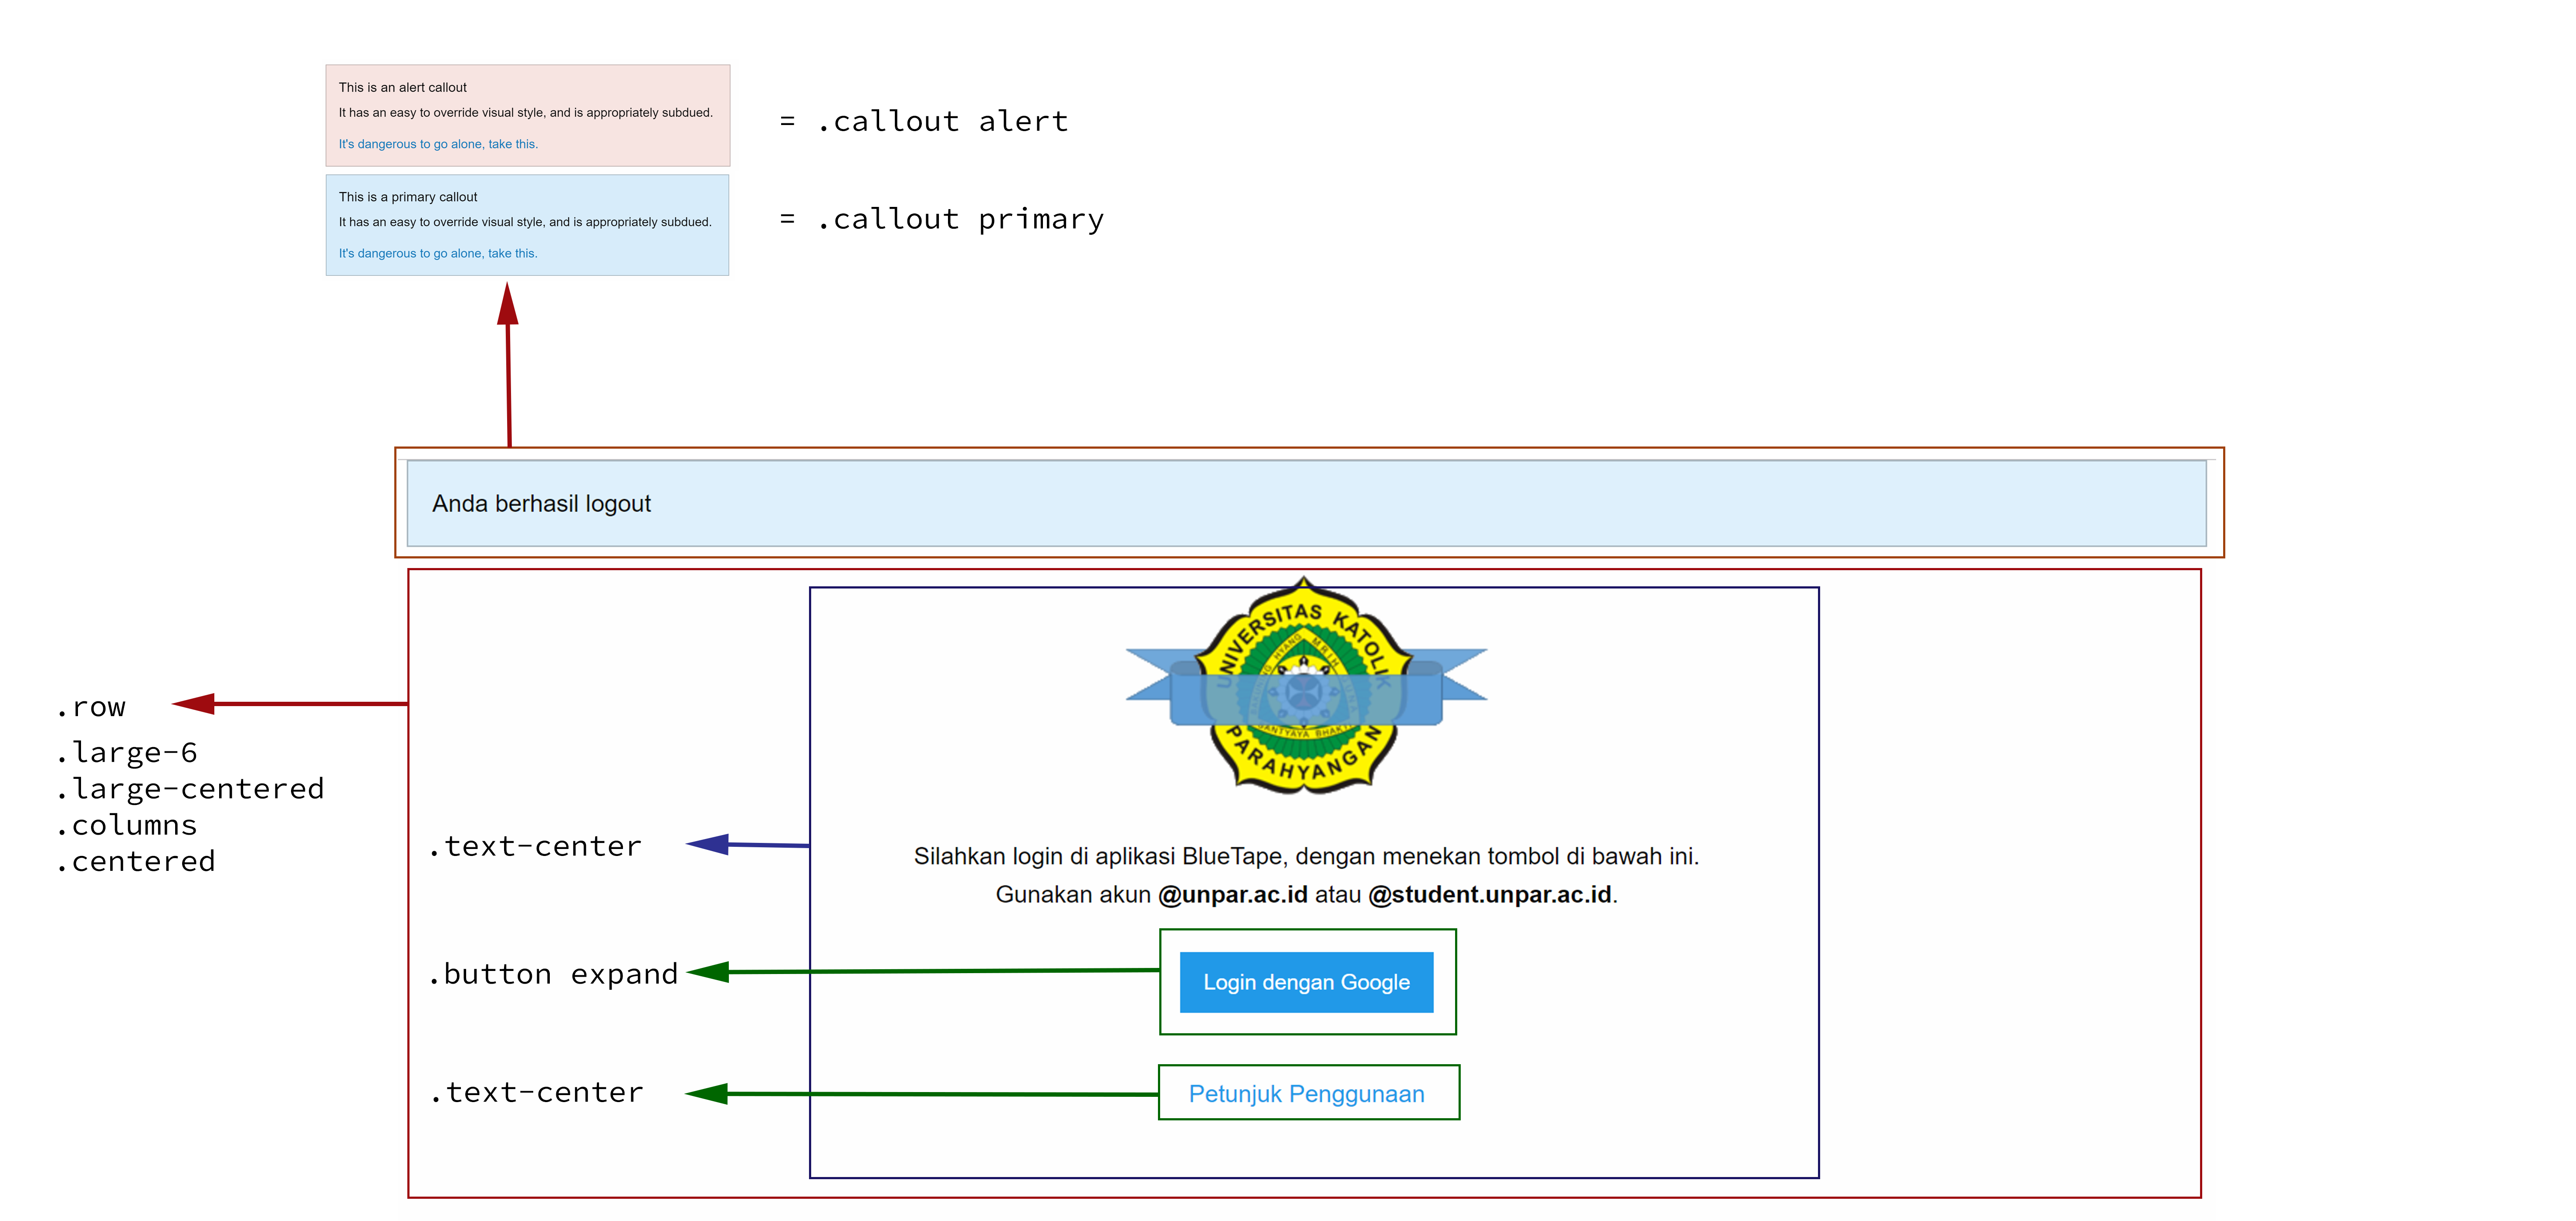
\includegraphics[width=\textwidth,height=\textheight,keepaspectratio]{foundation/analisis_login.png} 
	\caption{Analisis halaman login.} 
	\label{fig:analisisLogin}
\end{figure} 

Kelas yang digunakan pada halaman login (gambar ~\ref{fig:analisisLogin}) tertera pada tabel ~\ref{table:analisisLogin}:\\

\begin{table}[H]
	\centering
	\caption{Penggunaan kelas pada halaman login.}
	\begin{tabularx}{\textwidth}{lX}
		\toprule
		Kelas     & Penggunaan \\
		\midrule
		\texttt{.row, .large-6, .column} & Bagian konten akan terletak di tengah halaman utama yang memiliki lebar 6 grid.  \\
 		\texttt{.text-center} & Kalimat "Silahkan login .." dan link "Petunjuk Bagian" akan terletak ditengah container.\\
		\texttt{.button expand} & Tombol "Login dengan Google" akan memiliki \textit{styling} grid yang lebarnya memenuhi panjang grid nya.\\
		\bottomrule
	\end{tabularx}%	
	\label{table:analisisLogin}
\end{table} \noindent \\

\noindent Pada bagian atas halaman login terdapat notifikasi bagi user saat proses login dan logout. Kelas yang digunakan tertera pada tabel ~\ref{table:notifikasiUser}.\\

\begin{table}[H]
	\centering
	\caption{Penggunaan kelas pada bagian notifikasi user.}
	\begin{tabularx}{\textwidth}{lX}
		\toprule
		Kelas     & Penggunaan \\
		\midrule
		\texttt{.callout primary} & Notifikasi berwarna biru menandakan user berhasil \textit{login}.\\
		\texttt{.callout alert} & Notifikasi berwarna merah menandakan user berhasil \textit{logout}.\\
		\bottomrule
	\end{tabularx}%	
	\label{table:notifikasiUser}
\end{table}%


\subsection{Menu Navigasi}
Komponen menu navigasi digunakan pada keseluruhan tampilan website, bentuk menu akan menyesuaikan sesuai dengan layar dimana website diakses. \\
Berikut ini gambar ~\ref{fig:navigasiLarge} merupakan hasil penggunaan dari implementasi menu navigasi:

\begin{figure} [H]
	\centering  
	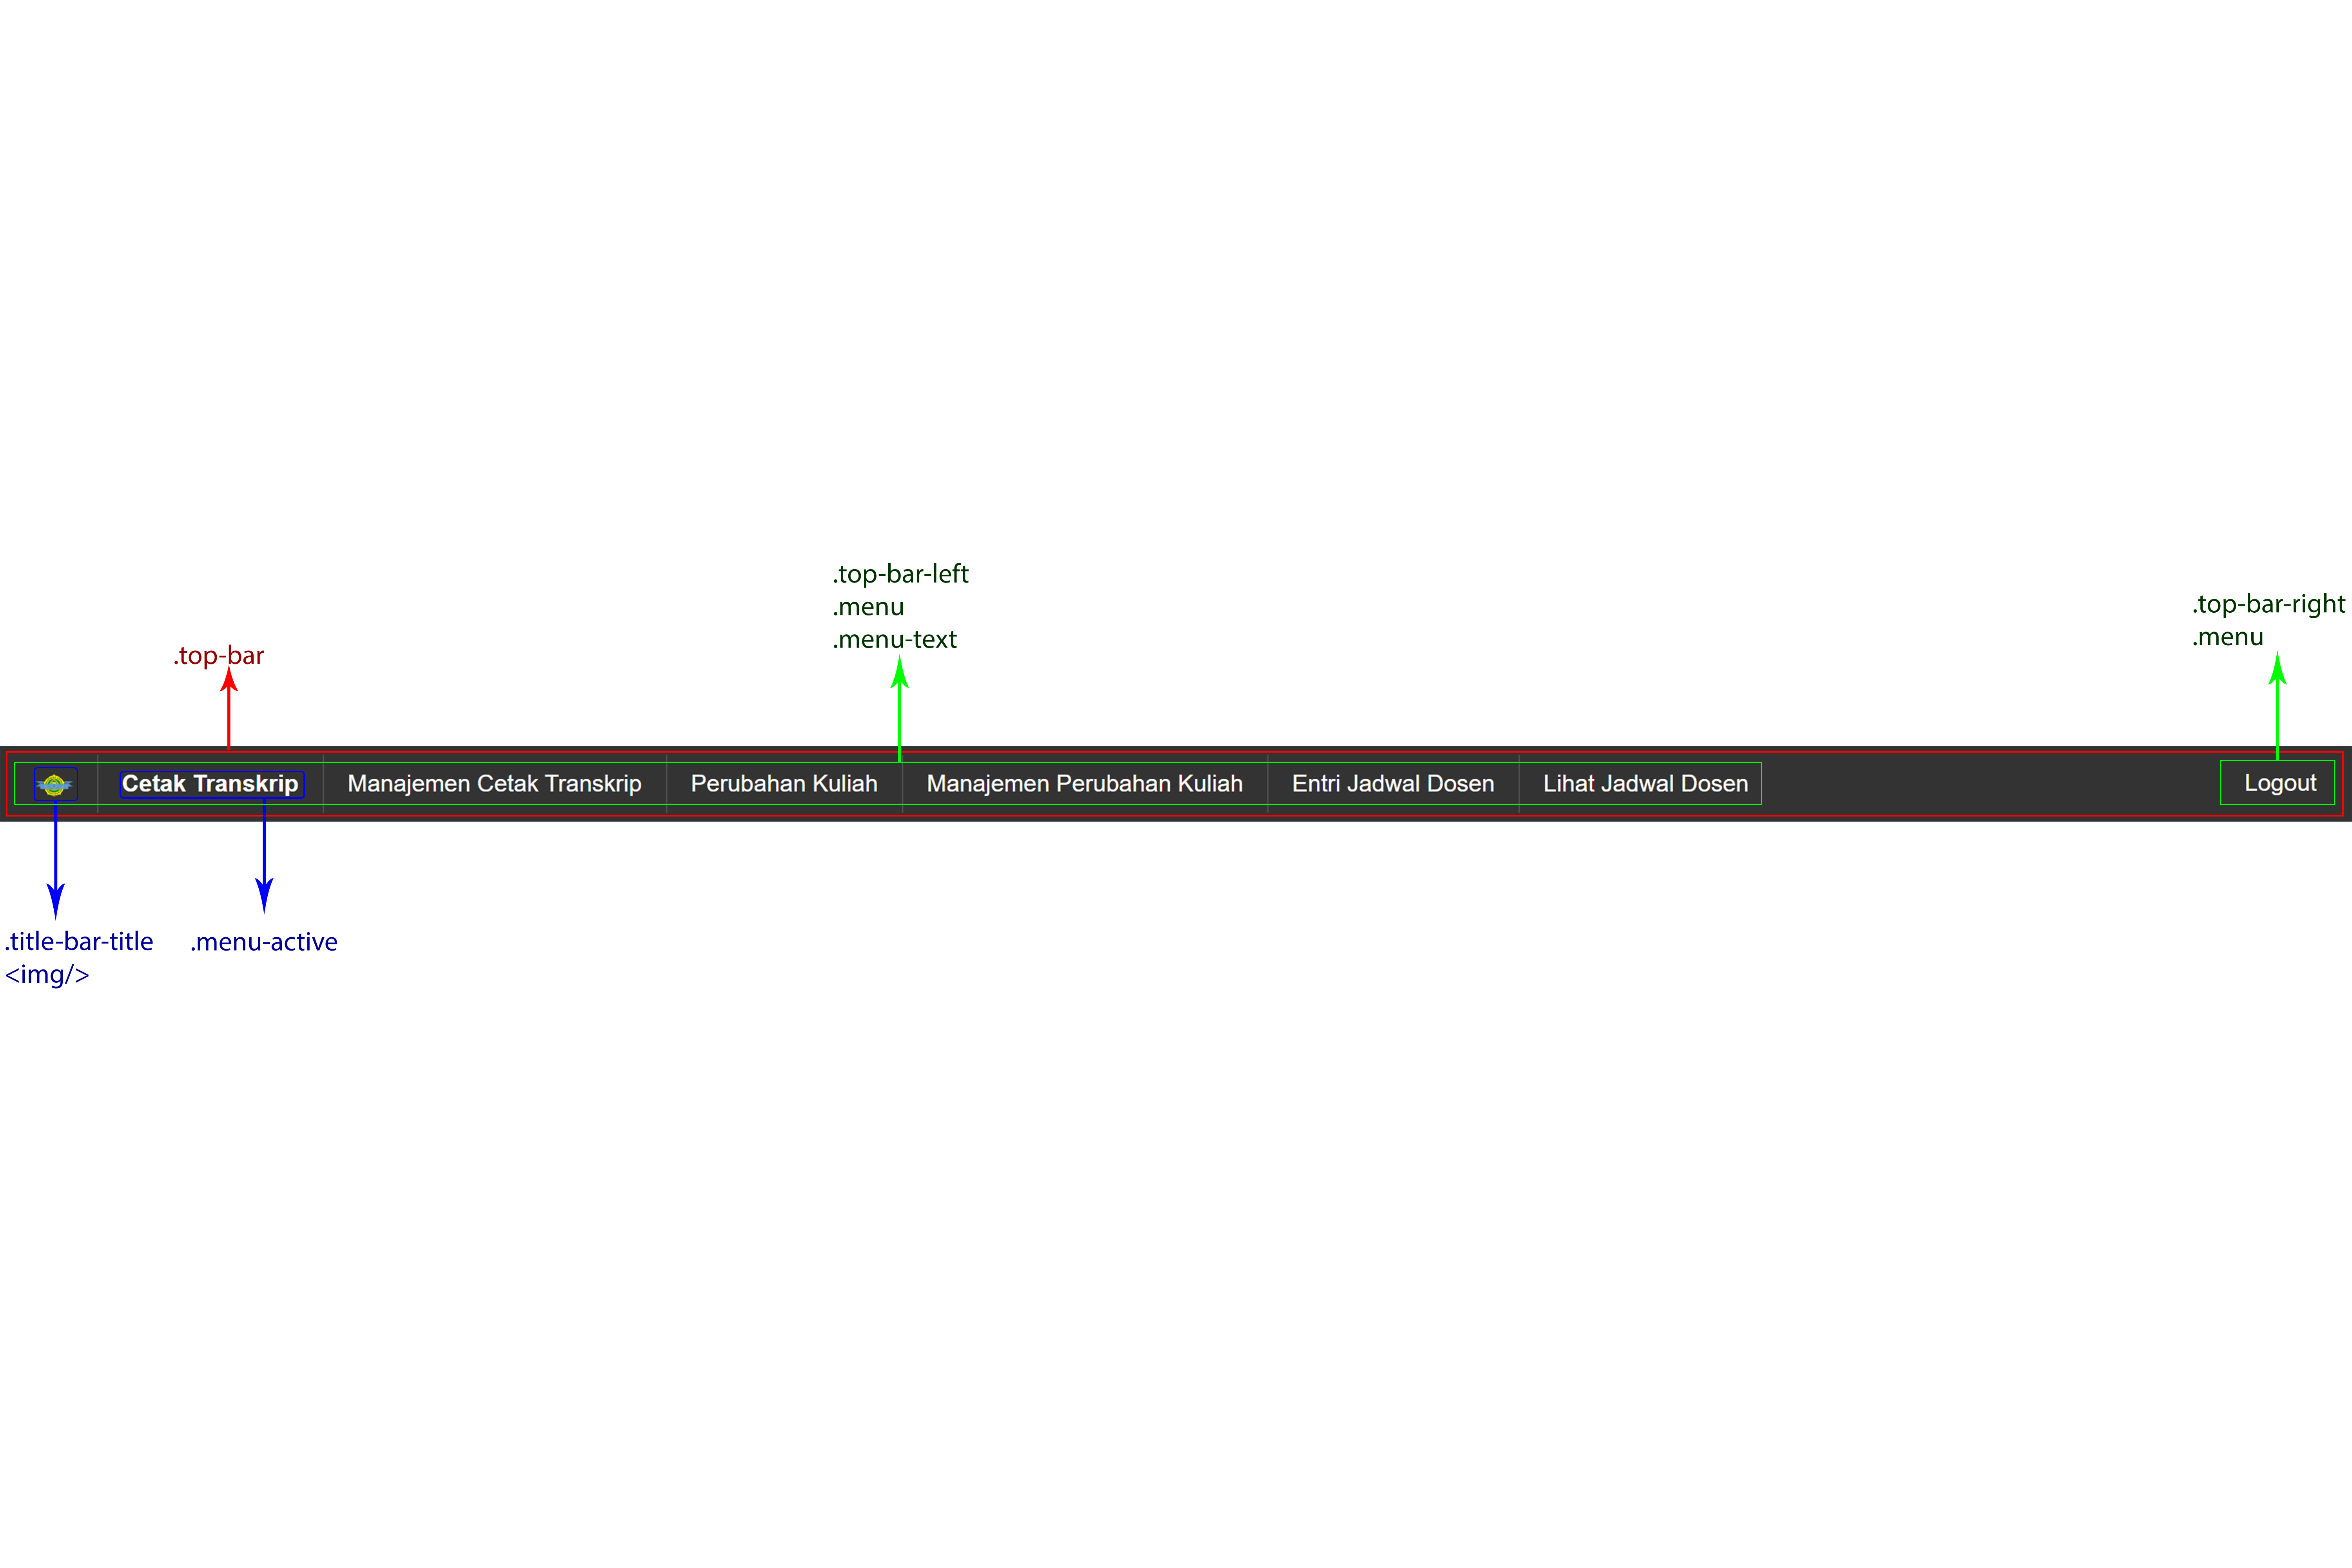
\includegraphics[width=\textwidth,height=\textheight,keepaspectratio]{foundation/analisis_top_bar.png}  
	\caption{Analisis menu navigasi di layar \textit{large}.} 
	\label{fig:navigasiLarge}
\end{figure}
Tabel ~\ref{table:navigasiLarge} menjelaskan kelas-kelas yang digunakan pada menu navigasi di layar \textit{large} .\\
\begin{table}[H]
	\centering
	\caption{Penggunaan kelas pada menu navigasi di layar \textit{large}.}
	\begin{tabularx}{\textwidth}{lX}
		\toprule
		Kelas     & Penggunaan \\
		\midrule
		\texttt{.top-bar}	 & Menu akan terletak pada bagian atas dari halaman.\\	
		\texttt{.menu}	 & Kelas yang membuat daftar judul halaman website menjadi menu.\\
		\texttt{.menu-active} & Kelas untuk menandakan menu yang sedang dipilih user.\\
		\texttt{.menu-text} & Kelas untuk menyelaraskan nama menu berbentuk teks agar sejajar dengan \textit{navigation bar}.\\	
		\texttt{.top-bar-left} & Kelas yang mengatur daftar menu disebelah kiri.\\
		\texttt{.top-bar-right} & Kelas yang mengatur daftar menu disebelah kanan.\\
		\bottomrule
	\end{tabularx}%	
	\label{table:navigasiLarge}
\end{table}%

\noindent Lalu untuk layar \textit{medium} dan \textit{small} menggunakan komponen \texttt{Advanced Layout} pada gambar ~\ref{fig:navigasiMedium} dimana  daftar halaman website yang ada pada menu berada di mode \textit{hide} dan digantian oleh ikon menu. 

\begin{figure} [H]
	\centering  
	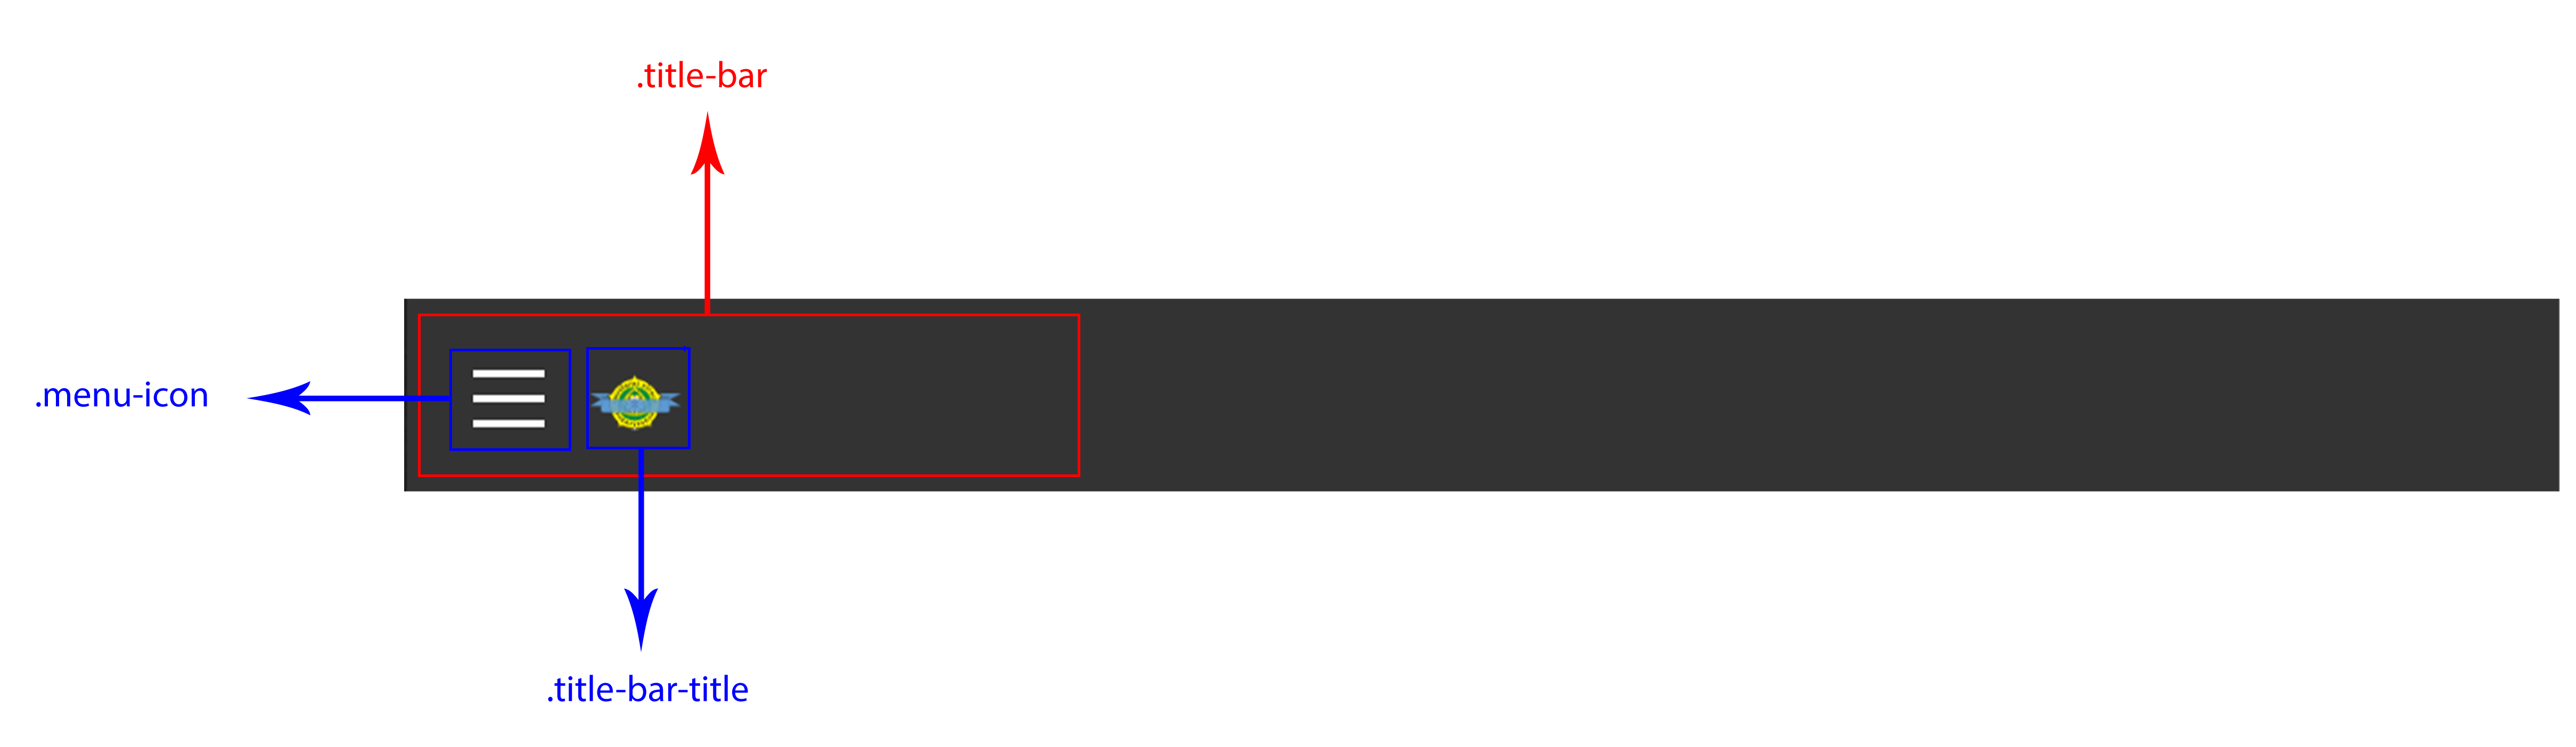
\includegraphics[width=\textwidth,height=\textheight,keepaspectratio]{foundation/analisis_top_bar_small.png} 
	\caption{Analisis menu navigasi di layar \textit{medium} dan \textit{small}.} 
	\label{fig:navigasiMedium}
\end{figure} \noindent

Komponen \texttt{Advanced Layout} terdiri dari kelas - kelas yang dijabarkan dalam tabel ~\ref{table:navigasiMedium}.\\

\begin{table}[H]
	\centering
	\caption{Penggunaan kelas pada menu navigasi di layar \textit{medium} dan \textit{small}.}
	\begin{tabularx}{\textwidth}{lX}
		\toprule
		Kelas     & Penggunaan \\
		\midrule
		\texttt{.title-bar}  & Kelas yang mendefinisikan penggunaan menu dari \textit{Advanced Layout}.\\
		\texttt{.title-bar-title}	 & Kelas yang mendefinisikan ikon BlueTape sebagai judul website.\\		
		\texttt{.menu-icon} & Kelas untuk menampilkan icon menu.\\			
		%belum ada di analisis
		\texttt{data-responsive-toggle} & Atribut untuk membuat daftar menu responsive.\\
		\texttt{data-toggle} & Atribut ini akan memanggil data yang disimpan dalam \texttt{data-toggle}.\\	
		\texttt{data-hide-for} & Atribut yang mengatur kapan menu navigasi akan responsif.\\
		\bottomrule
	\end{tabularx}%	
	\label{table:navigasiMedium}
\end{table}% 

\subsection{Halaman Permintaan Cetak Transkrip}
\subsubsection{Halaman Utama}

\par Halaman permintaan cetak transkrip terdiri dari dua konten yaitu: "Permohonan Baru" dan "Histori Permohonan". Setiap konten akan dipisahkan dengan border. Pada konten "Permohonan Baru" terdiri dari sebuah form yang berisi \textit{field} yang terdiri dari 2 \textit{rows} dan sebuah tombol "Kirim Permohonan". Lalu konten "Histori Permohonan" terdiri dari sebuah tabel dimana data akan dipanggil dari \textit{database}.  dan kolom 'Aksi' menngarahkan \textit{user} ke sebuah modal lihat permintaan transkrip yang direpresentasikan dengan ikon mata.\\ \\
Berikut ini gambar ~\ref{fig:analisisCetakTranskrip} merupakan hasil penggunaan dari implementasi menu navigasi:

\begin{figure} [H]
	\centering  
	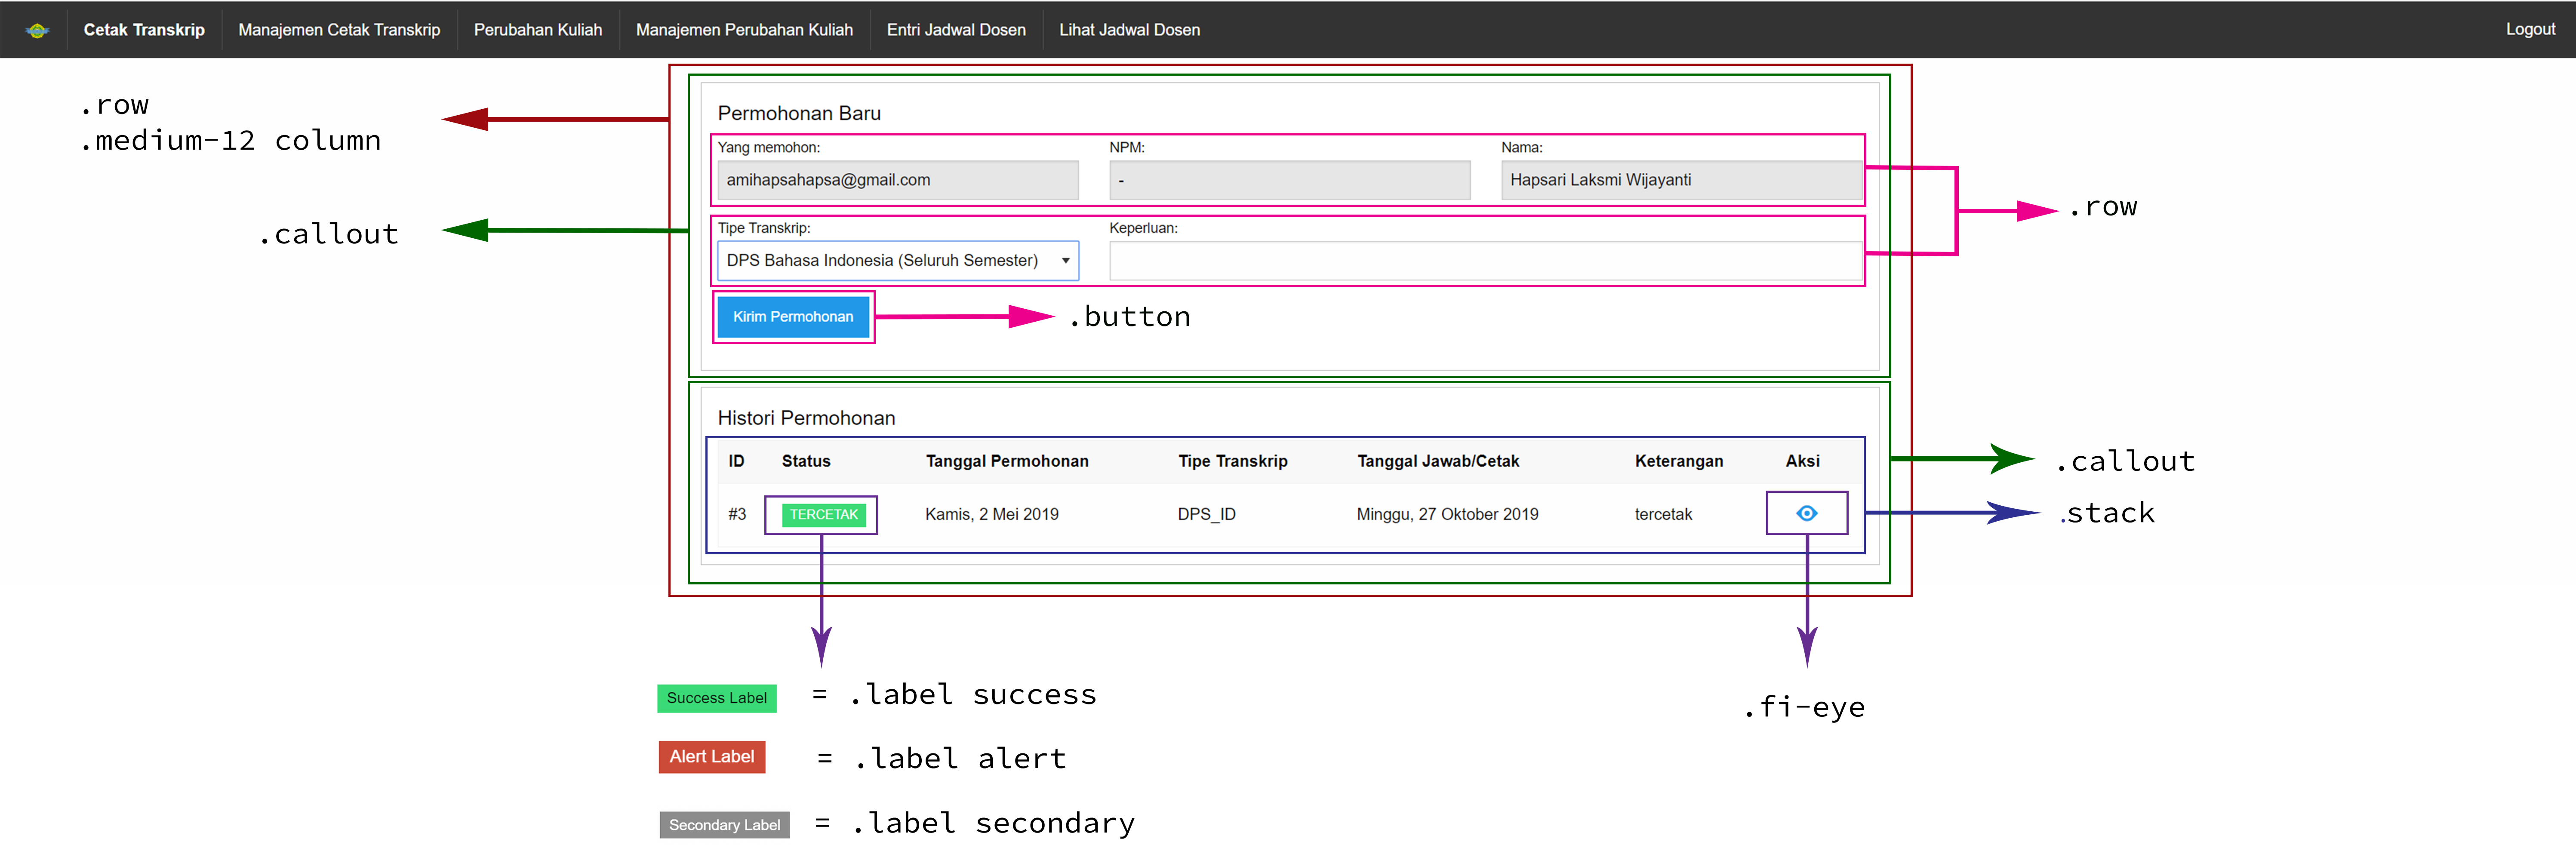
\includegraphics[width=\textwidth,height=\textheight,keepaspectratio]{foundation/analisis_mahasiswa_cetak_transkrip.png}
	\caption{Analisis halaman cetak transkrip.} 
	\label{fig:analisisCetakTranskrip}
\end{figure} 
\noindent Kelas yang digunakan dalam konten permohonan baru tertera pada tabel ~\ref{table:analisisCetakTranskrip}.\\

\begin{table}[H]
	\centering
	\caption{Penggunaan kelas pada halaman utama cetak transkrip.}
	\begin{tabularx}{\textwidth}{lX}
		\toprule
		Kelas     & Penggunaan \\
		\midrule
		\texttt{.row} & Kelas ini digunakan untuk menyimpan container menjadi satu \textit{cell} dan mengatur \textit{field-form} menjadi satu baris. \\
		\texttt{.medium-12 column}& Keseluruhan konten akan memiliki lebar 12 grid pada layar medium.\\
		\texttt{.button} & Jenis kelas yang digunakan pada tombol `Kirim Permohonan'\\
		\texttt{.callout} & Untuk membuat border yang memisahkan konten permohonan baru dan histori permohonan.\\
		\texttt{.fi-eye}& Kelas pada font awesome untuk link ke modal lihat.\\		
		\texttt{.stack} & Tabel lihat cetak transkrip dengan lebar yang dapat disesuaikan berdasarkan ukuran layar.\\
		\bottomrule
	\end{tabularx}%	
	\label{table:analisisCetakTranskrip}
\end{table} \\ 

\noindent Tabel ~\ref{table:labelCetakTranskrip} menjabarkan pada kolom 'status' digunakan highlight yang terdiri dari tiga warna. Kelas yang digunakan adalah \texttt{.label}.\\

\begin{table}[H]
	\centering
	\caption{Penggunaan komponen label pada kolom status.}
	\begin{tabularx}{\textwidth}{lX}
		\toprule
		Kelas & Penggunaan \\
		\midrule
		\texttt{.label success} & Label hijau menandakan transkrip yang telah tercetak.\\
		\texttt{.label alert} & Label merah menandakan yang gagal tercetak.\\
		\texttt{.label secondary} & Label abu-abu menandakan transkrip belum tercetak.\\
		\bottomrule
	\end{tabularx}%	
	\label{table:labelCetakTranskrip}
\end{table}%

\subsubsection{Modal: Lihat}
Gambar ~\ref{fig:analisisModalLihatPermintaanCetakTranskrip} implementasi apabila user memilih ikon mata, maka website akan mengarahkan ke modal lihat permintaan cetak transkrip.  \\
\begin{figure} [H]
	\centering  
	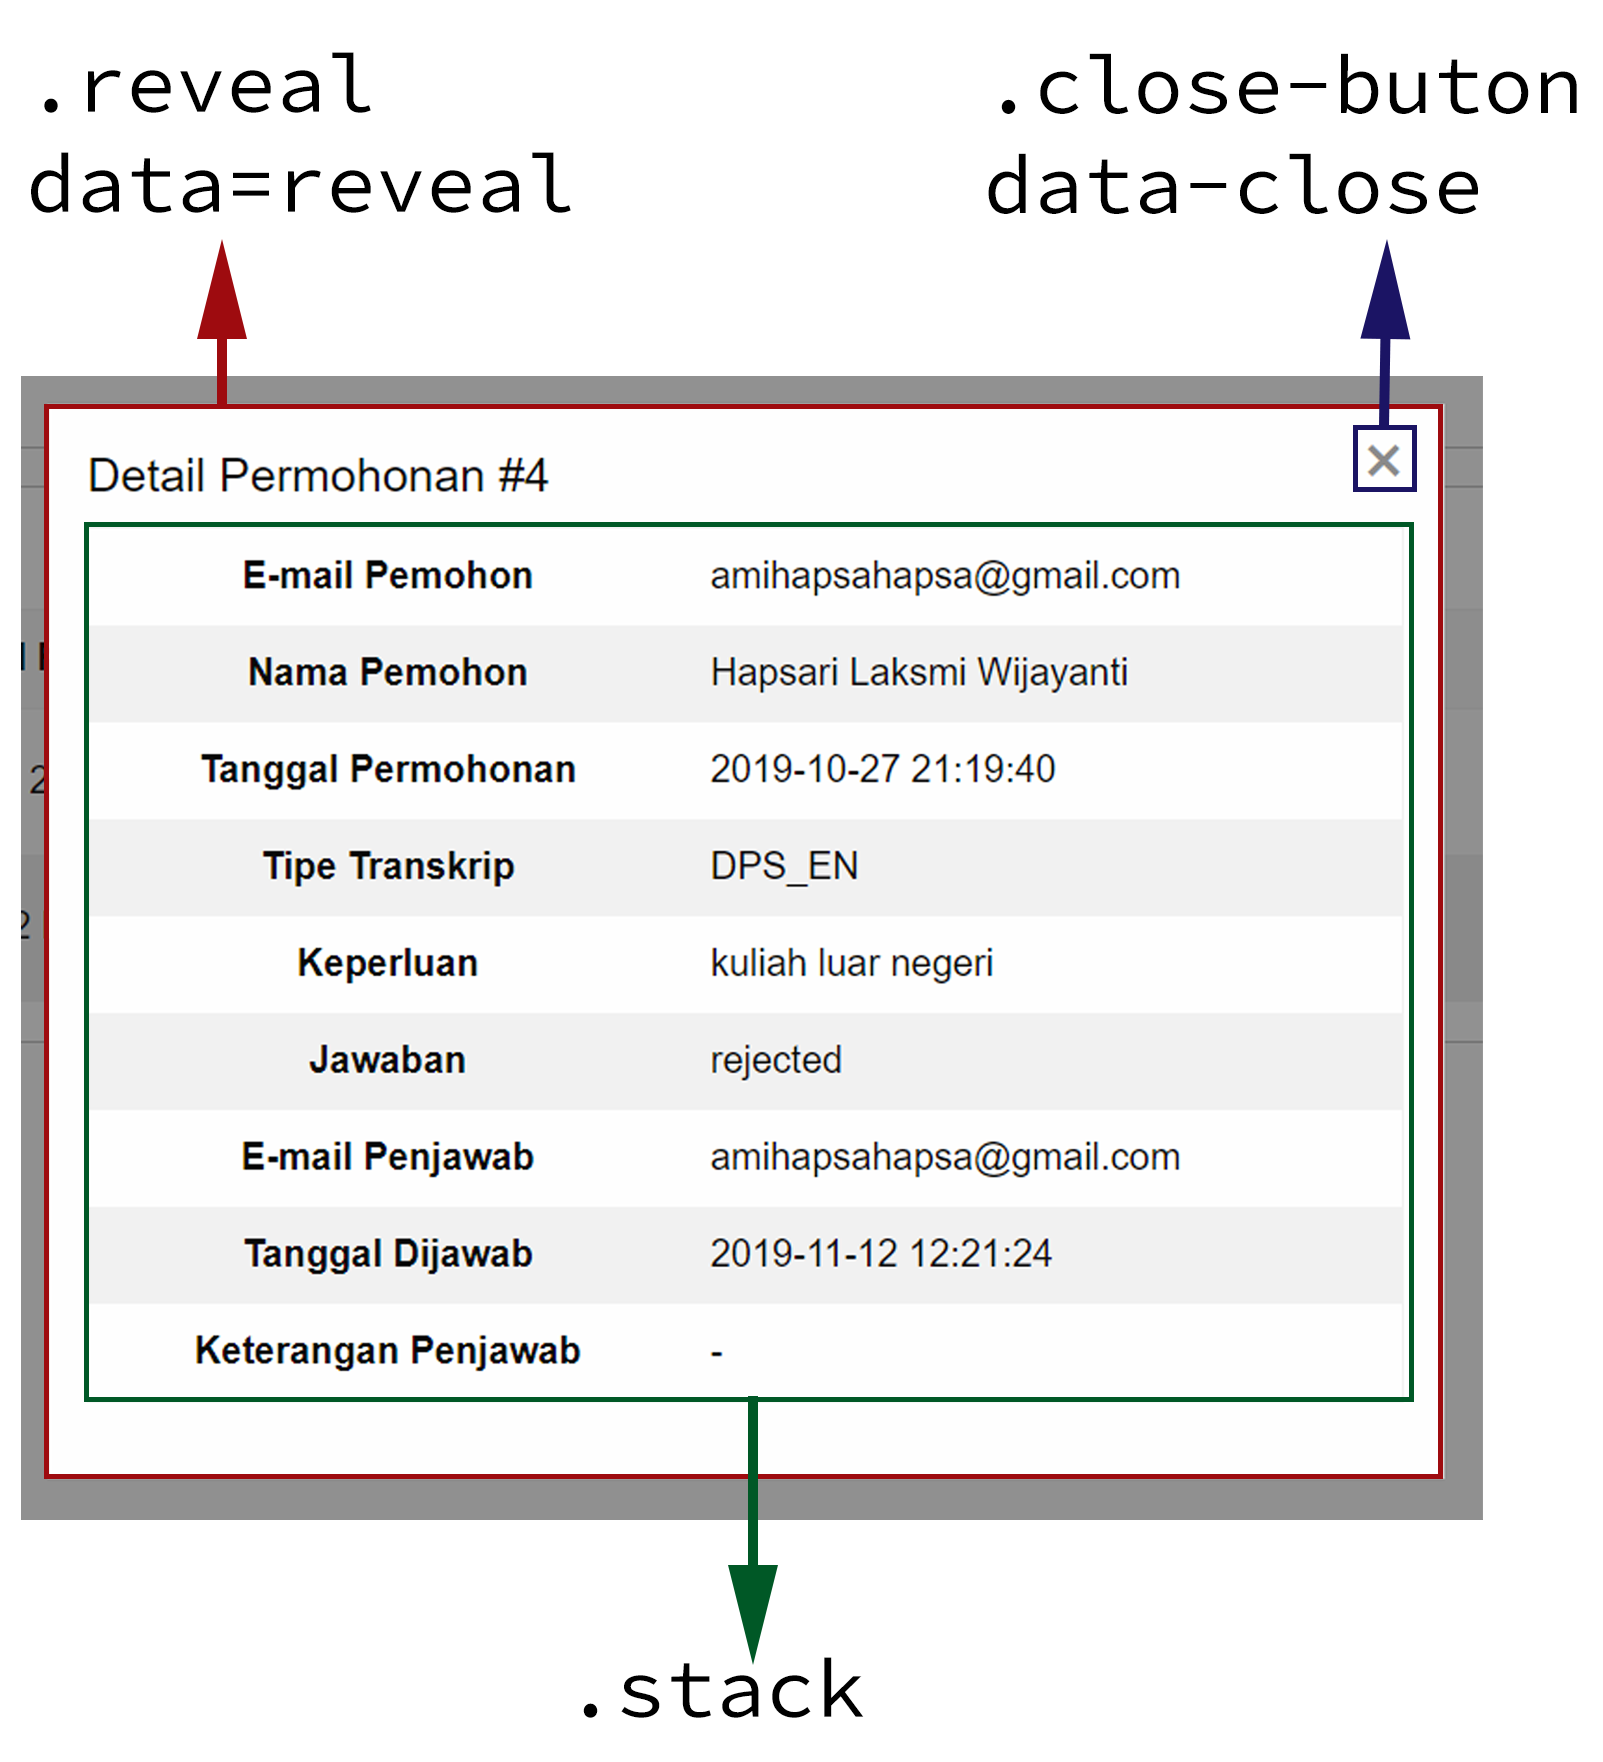
\includegraphics[width=0.4\textwidth,height=\textheight,keepaspectratio]{foundation/analisis_modal_eye_cetak_transkrip.png}  
	\caption{Analisis modal lihat permintaan cetak transkrip.} 
	\label{fig:analisisModalLihatPermintaanCetakTranskrip}
\end{figure}

\noindent Modal akan menampilkan detail permohonan cetak transkrip berdasarkan ID yang tercatat. Kelas yang digunakan pada modal lihat tertera pada tabel ~\ref{table:analisisModalLihatPermintaanCetakTranskrip}. \\

\begin{table}[H]
	\centering
	\caption{Penggunaan kelas pada modal lihat permintaan transkrip.}
	\begin{tabularx}{\textwidth}{lX}
		\toprule
		Kelas & Penggunaan \\
		\midrule
		\texttt{.reveal data-reveal} & Kelas yang menampilkan modal lihat cetak transkrip. \\
		\texttt{.close-button data-close} & Kelas yang memungkinkan \textit{user} untuk menutup halaman modal.\\
		\texttt{.stack} & Kelas untuk membuat tabel detail permohonan.\\
		\bottomrule
	\end{tabularx}% 
	\label{table:analisisModalLihatPermintaanCetakTranskrip}
\end{table}%

\subsection{Halaman Manajemen Cetak Transkrip}
Halaman ini terdiri dari satu konten yaitu "Permintaan Transkrip" tertera pada gambar ~\ref{fig:analisisManajemenCetakTranskrip}. Bagian form pencarian NPM menggunakan \textit{group field}, dimana nama form , isi form dan tombol merupakan satu kesatuan. Lalu dibawah form terdapat tabel yang menampilkan data permintaan cetak transkrip. 
\subsubsection{Halaman Utama}
\begin{figure} [H]
	\centering  
	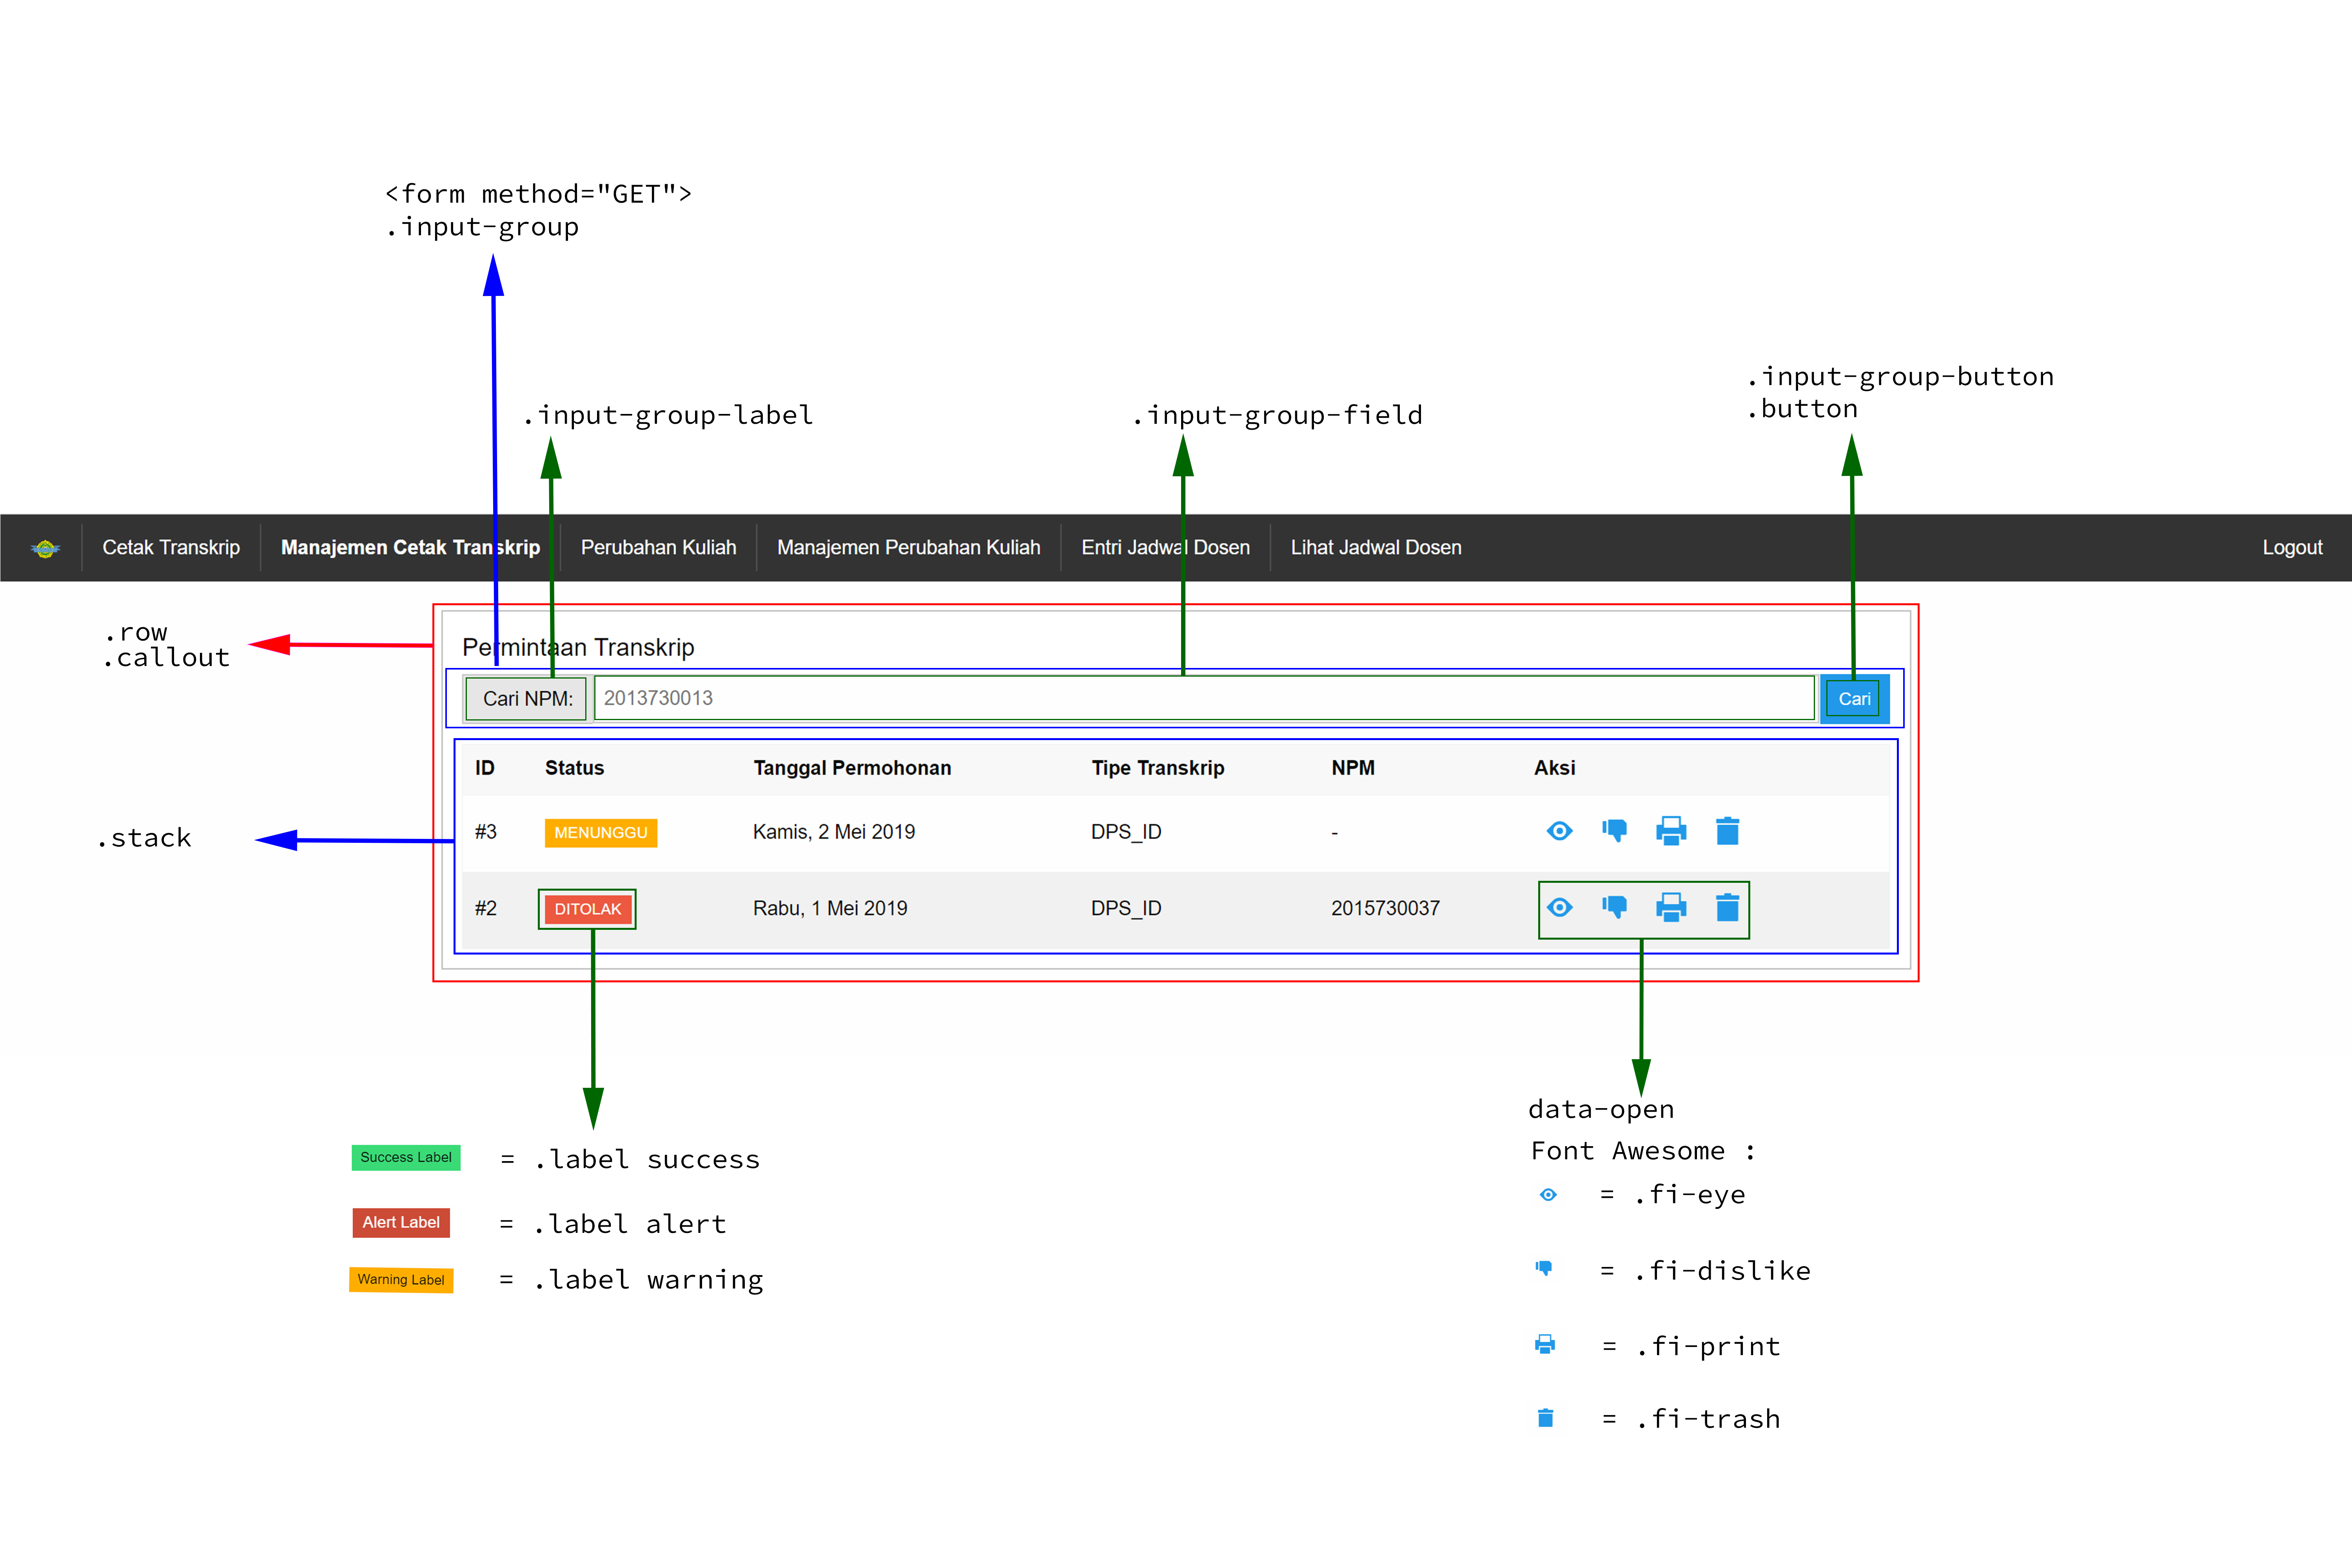
\includegraphics[width=\textwidth,height=\textheight,keepaspectratio]{foundation/analisis_manajemen_cetak_transkrip.png}
	\caption{Analisis manajemen cetak transkrip.} 
	\label{fig:analisisManajemenCetakTranskrip}
\end{figure} 

Kelas yang digunakan dalam halaman ini tertera pada tabel ~\ref{table:analisisManajemenCetakTranskrip}:\\
\begin{table}[H]
	\centering
	\caption{Penggunaan kelas pada halaman manajemen cetak transkrip.}
	\begin{tabularx}{\textwidth}{lX}
		\toprule
		Kelas     & Penggunaan \\
		\midrule
		\texttt{.row} & Kelas ini memiliki dua fungsi sebagai container konten dan mengatur beberapa \textit{field-form} menjadi satu baris.\\
		\texttt{.callout} & Untuk membuat border yang memisahkan konten permohonan baru dan histori permohonan.\\
		\texttt{.stack} & Jenis tabel yang digunakan tabel histori permohonan, sehingga pada layar medium lebar tabel akan menyesuaikan kan tiap \textit{cell} ditampilkan secara bertumpuk.\\
		\bottomrule
	\end{tabularx}%	
	\label{table:analisisManajemenCetakTranskrip}
\end{table} \\

\noindent Pada tabel permintaan transkrip terdapat status permintaan transkrip yang di \textit{highlight} menggunakan warna yang berbeda - beda. Kelas yang digunakan tertera pada tabel ~\ref{table:analisisLabelManajemenCetakTranskrip}.\\

\begin{table}[H]
	\centering
	\caption{Penggunaan komponen label pada kolom status histori permohonan.}
	\begin{tabularx}{\textwidth}{lX}
		\toprule
		Kelas     & Penggunaan \\
		\midrule
		\texttt{.label success} & Label untuk transkrip yang telah tercetak.\\
		\texttt{.label alert} & Label untuk transkrip yang gagal tercetak.\\
		\texttt{.label warning} & Label untuk transkrip yang menunggu untuk tercetak.\\		
		\bottomrule
	\end{tabularx}%	
	\label{table:analisisLabelManajemenCetakTranskrip}
\end{table}%


\noindent Untuk kolom aksi, terdapat empat kelas dari Font Awesome. Setiap ikon mengarahkan \textit{user} ke halaman modal dan halaman \textit{preview} cetak transkrip. Kelas - kelas yang digunakan tertera pada tabel ~\ref{table:analisisFontAwesomeManajemenCetakTranskrip}.\\

\begin{table}[H]
	\centering
	\caption{Penggunaan kelas font awesome pada kolom aksi.}
	\begin{tabularx}{\textwidth}{lX}
		\toprule
		Kelas     & Penggunaan \\
		\midrule
		\texttt{fi-eye} & \textit{Hypertext reference} berbentuk ikon yang mengarahkan ke modal lihat transkrip.\\
		\texttt{fi-dislike} & \textit{Hypertext reference} berbentuk ikon yang mengarahkan ke modal tolak cetak transkrip.\\
		\texttt{fi-print} & \textit{Hypertext reference} berbentuk ikon yang mengarahkan ke modal print cetak transkrip.\\
		\texttt{fi-trash} & \textit{Hypertext reference} berbentuk ikon yang mengarahkan ke modal hapus permintaan transkrip.\\
		\bottomrule
	\end{tabularx}%	
	\label{table:analisisFontAwesomeManajemenCetakTranskrip}
\end{table} \\

\subsubsection{Modal: Lihat, Tolak, Print dan Hapus}

Bagian modal pada halaman manajemen cetak transkrip terdiri dari empat bagian.\\ \\ 
Gambar ~\ref{fig:analisisModalManajemenCetakTranskrip} menunjukan kelas yang digunakan untuk setiap modal:
\begin{figure}[h!]	
	\centering
	\begin{subfigure}[b]{0.25\linewidth}   
		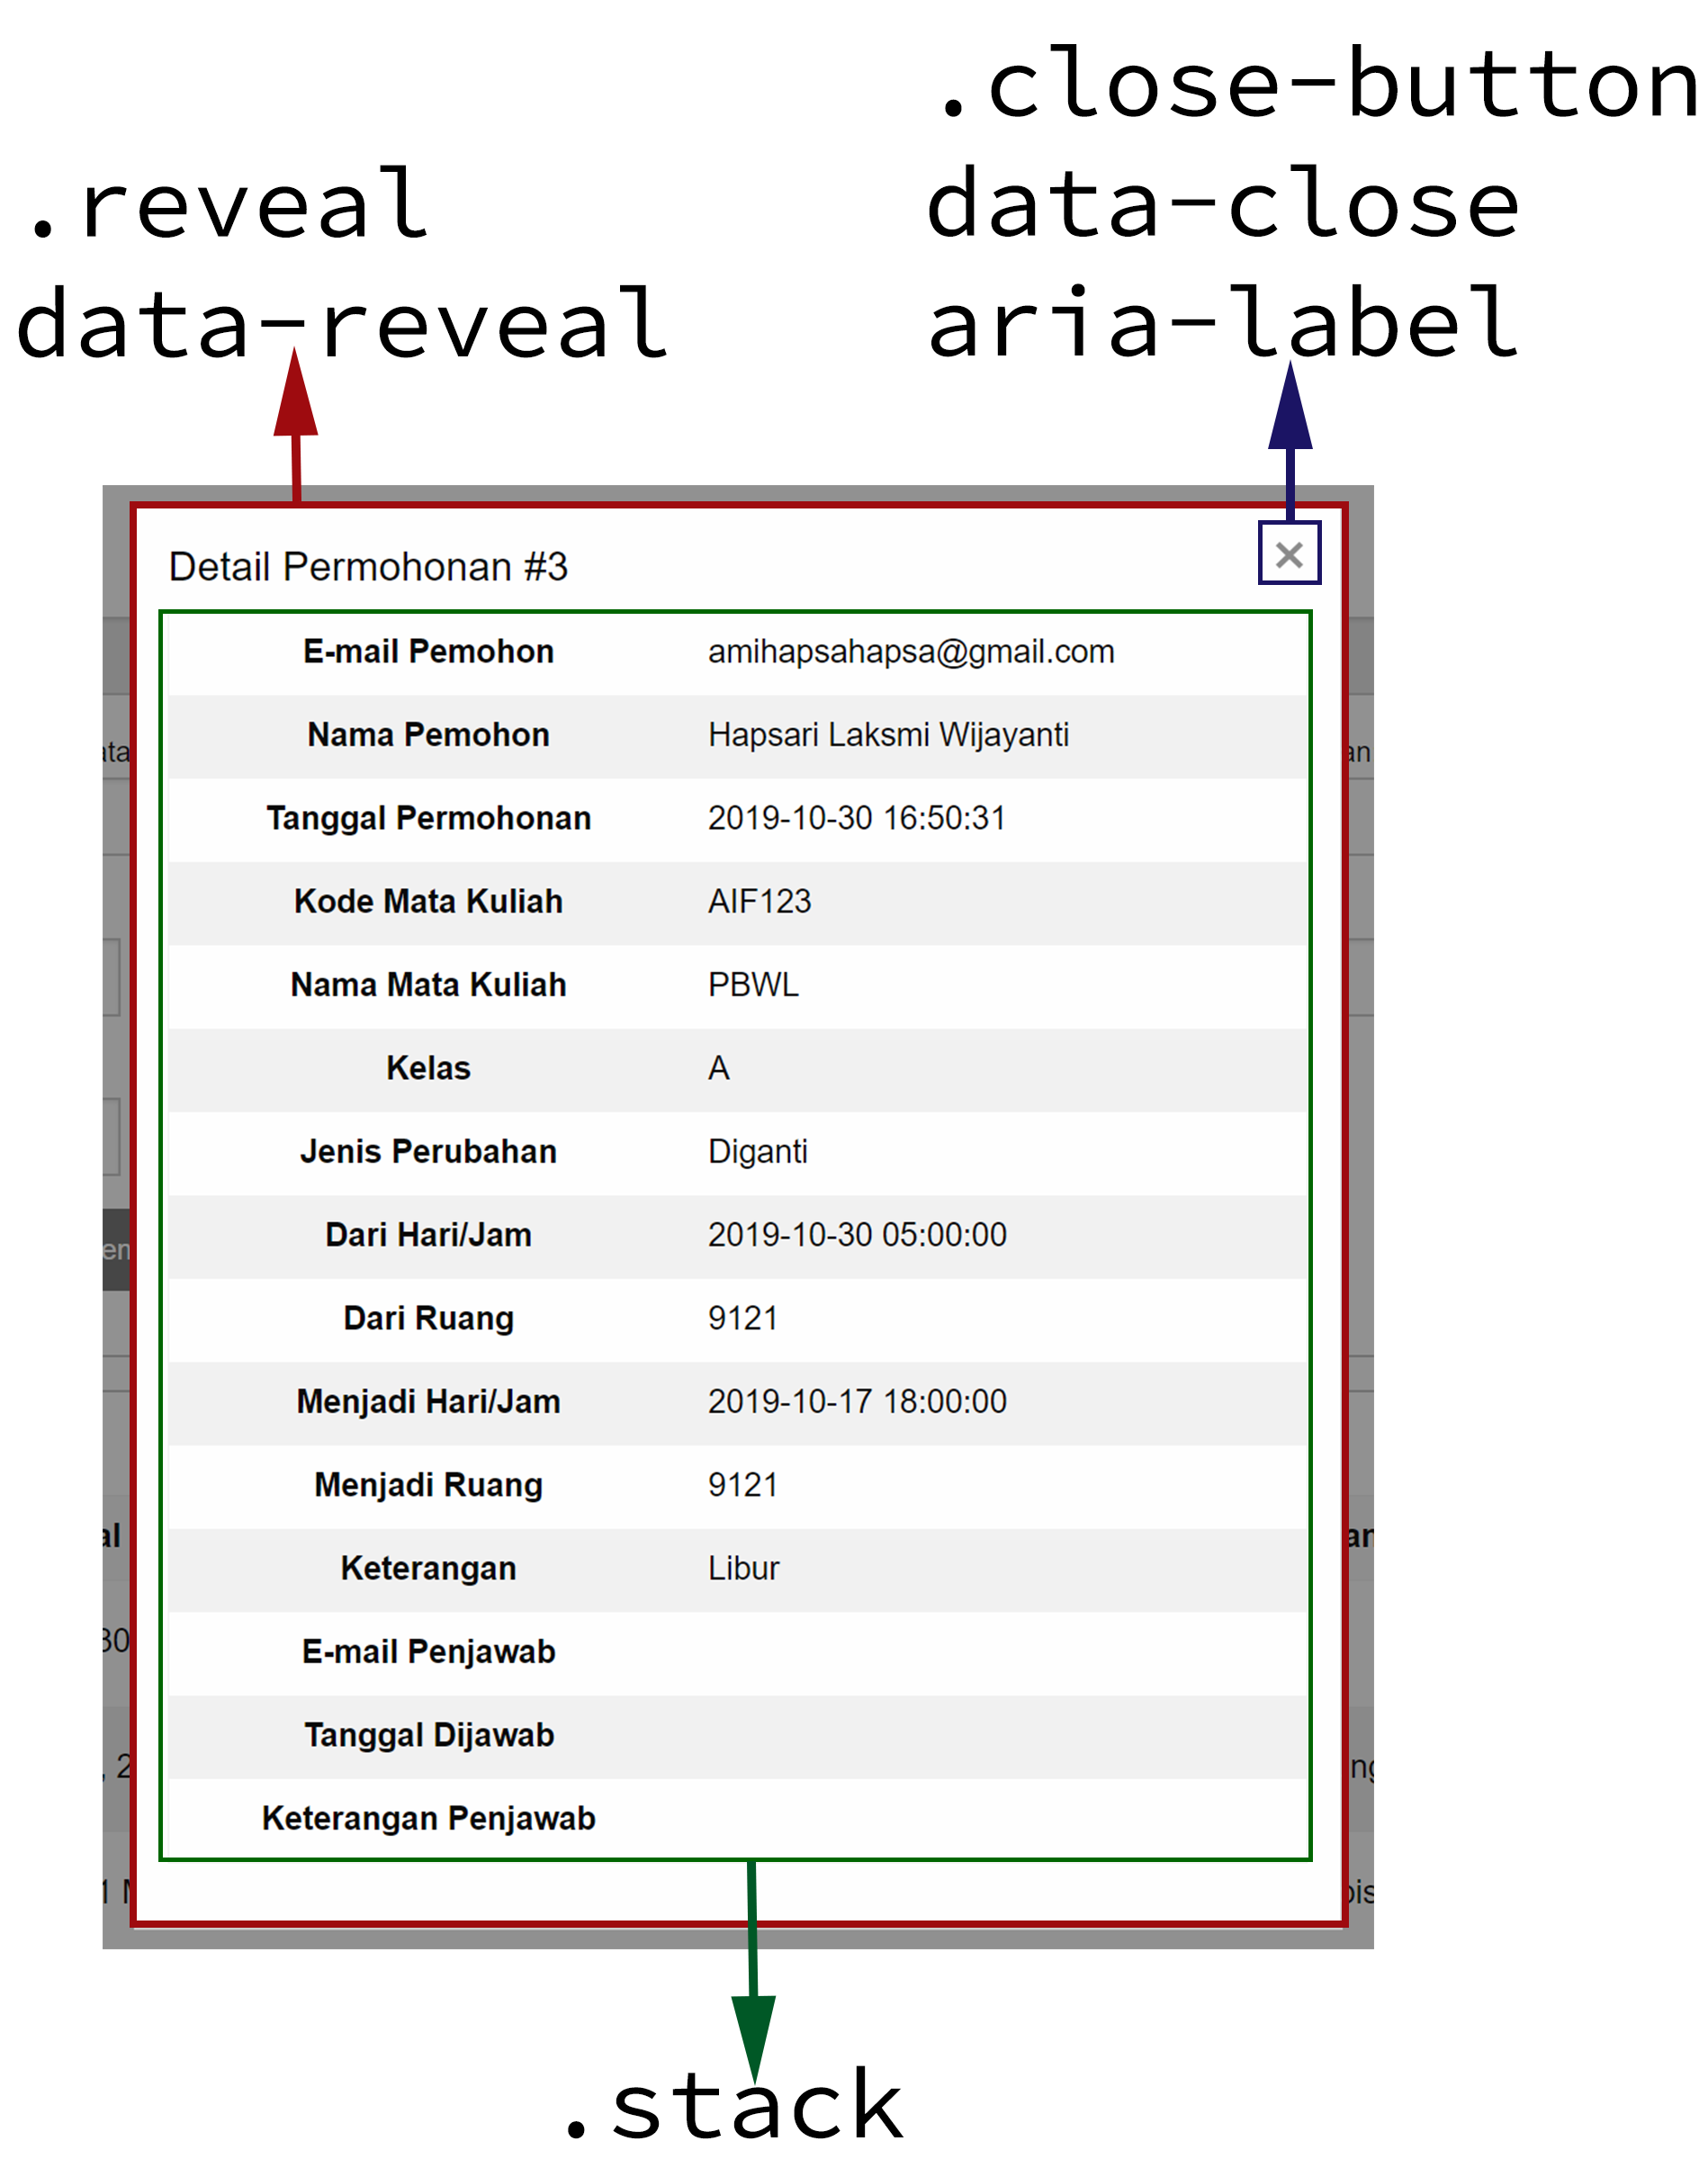
\includegraphics[width=\textwidth,height=\textheight,keepaspectratio]{foundation/analisis_modal_eye_manajemen_cetak_transkrip.png}
		\caption{Modal lihat.}
	\end{subfigure}
	\begin{subfigure}[b]{0.45\linewidth} 
		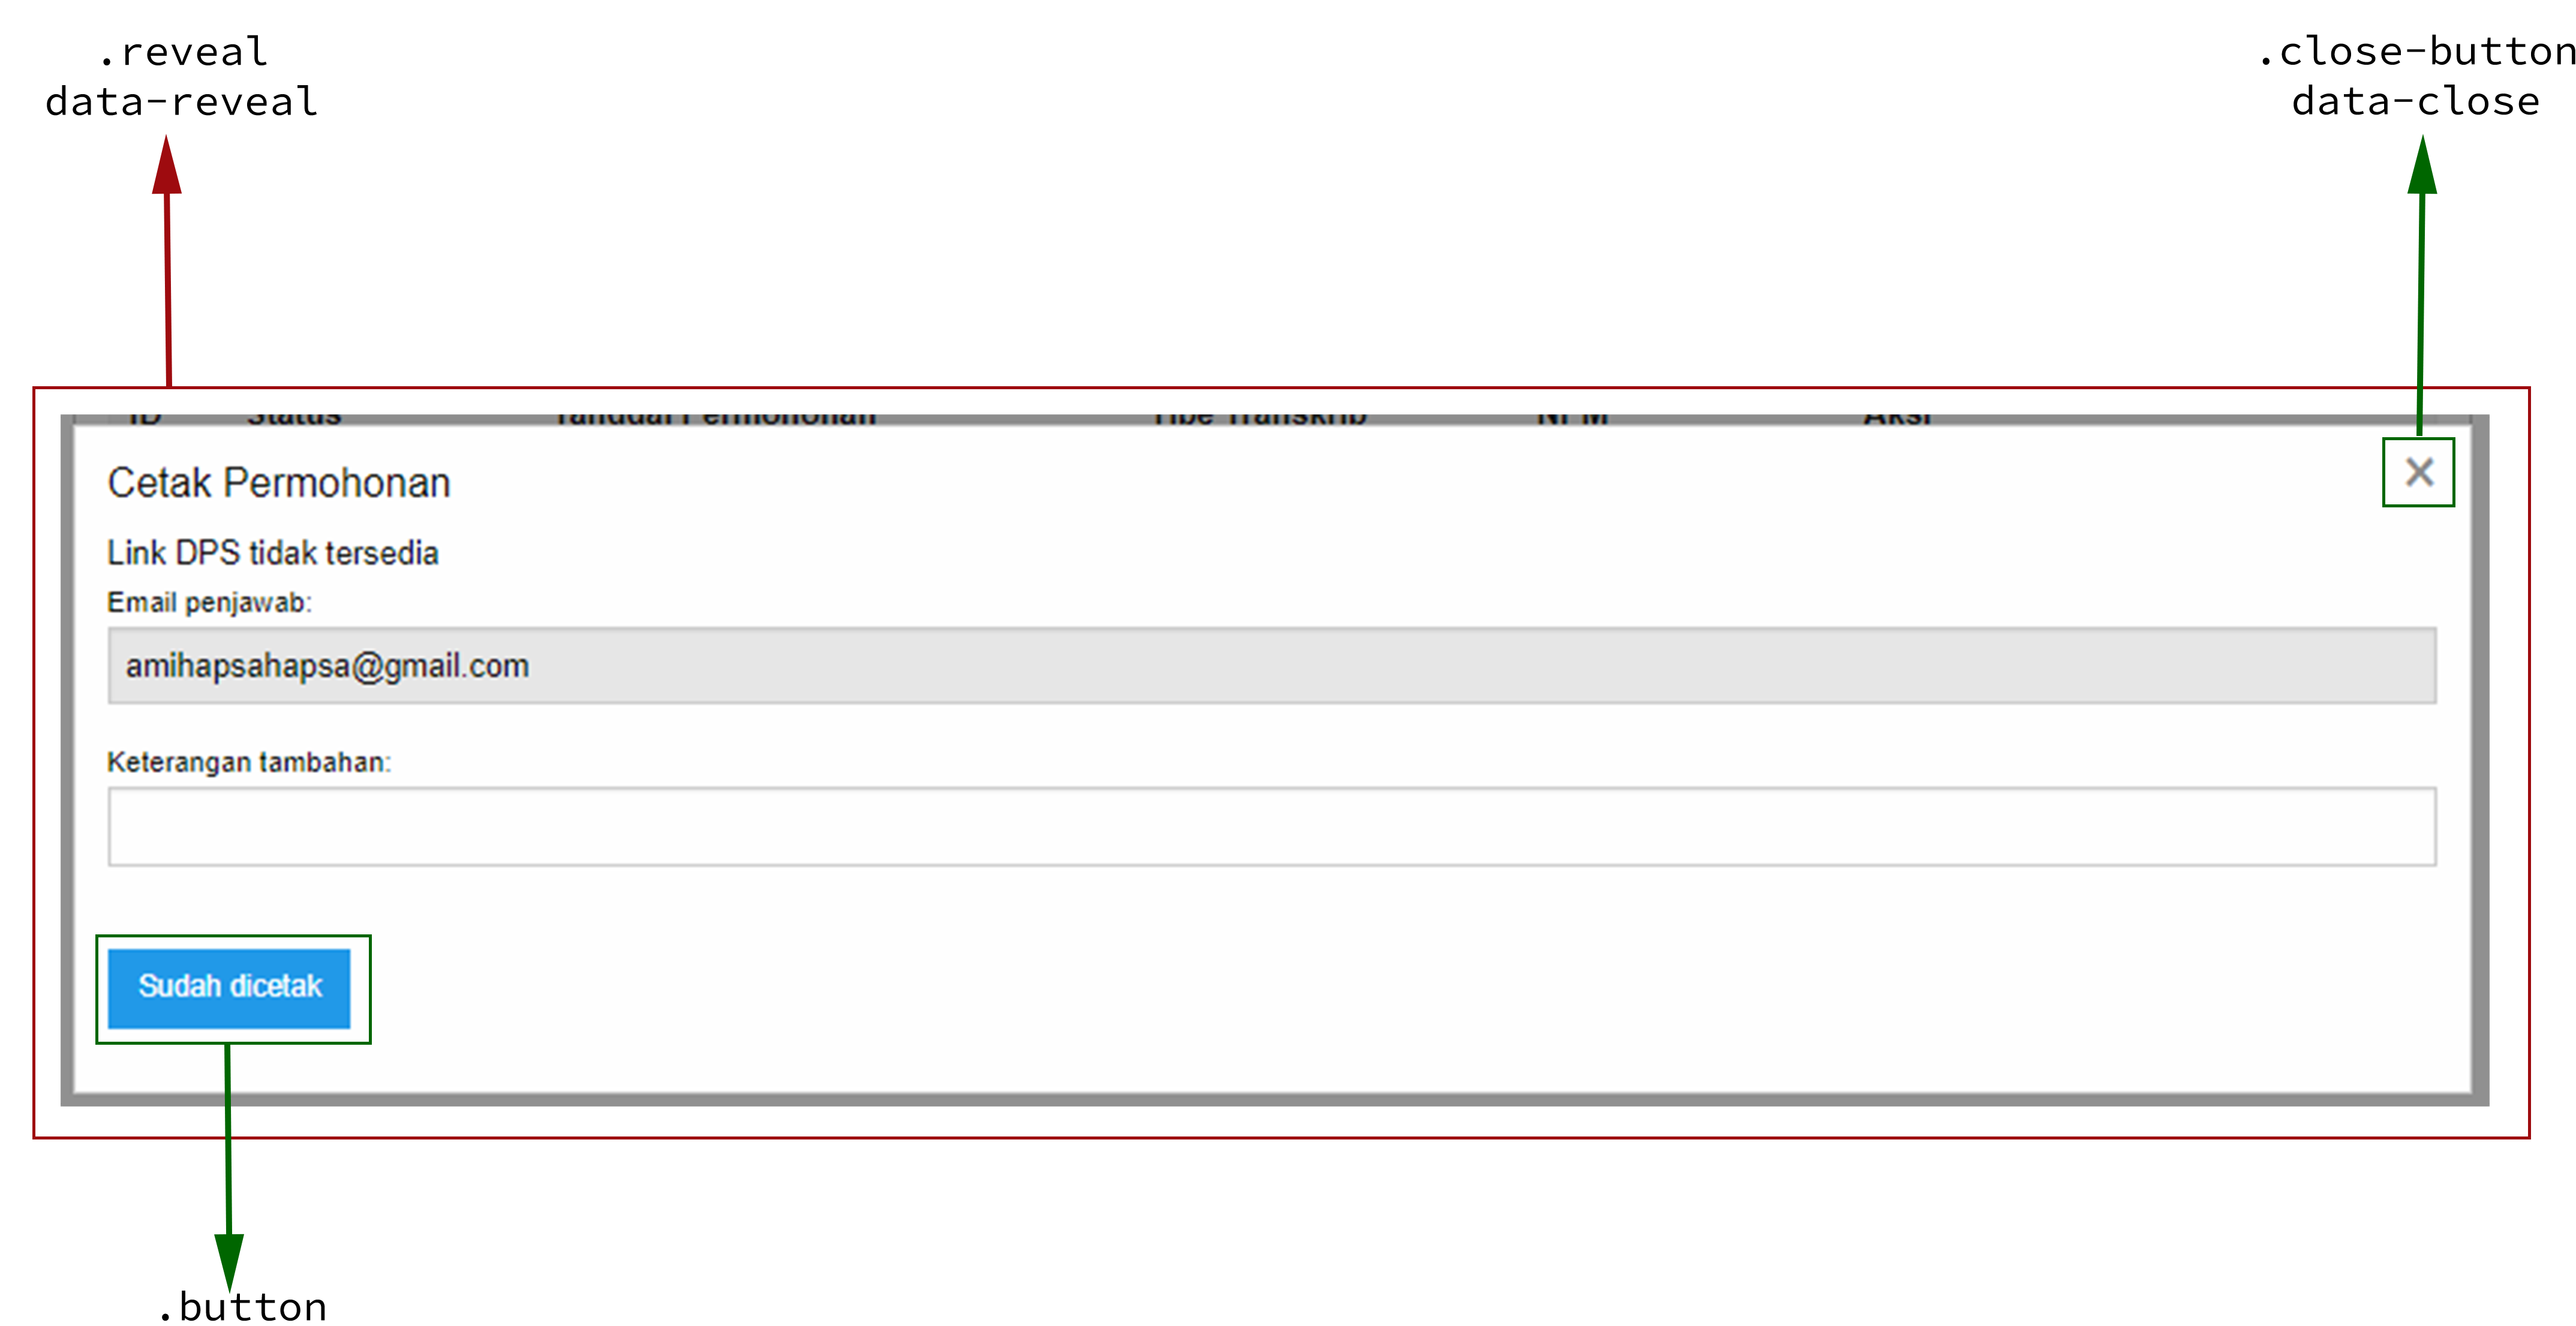
\includegraphics[width=\textwidth,height=\textheight,keepaspectratio]{foundation/analisis_modal_print_manajemen_cetak_transkrip.png}
		\caption{Modal print.} 
	\end{subfigure}
\end{figure}
\begin{figure}[h!]
	\centering
	\ContinuedFloat	
	\begin{subfigure}[b]{0.45\linewidth}  
		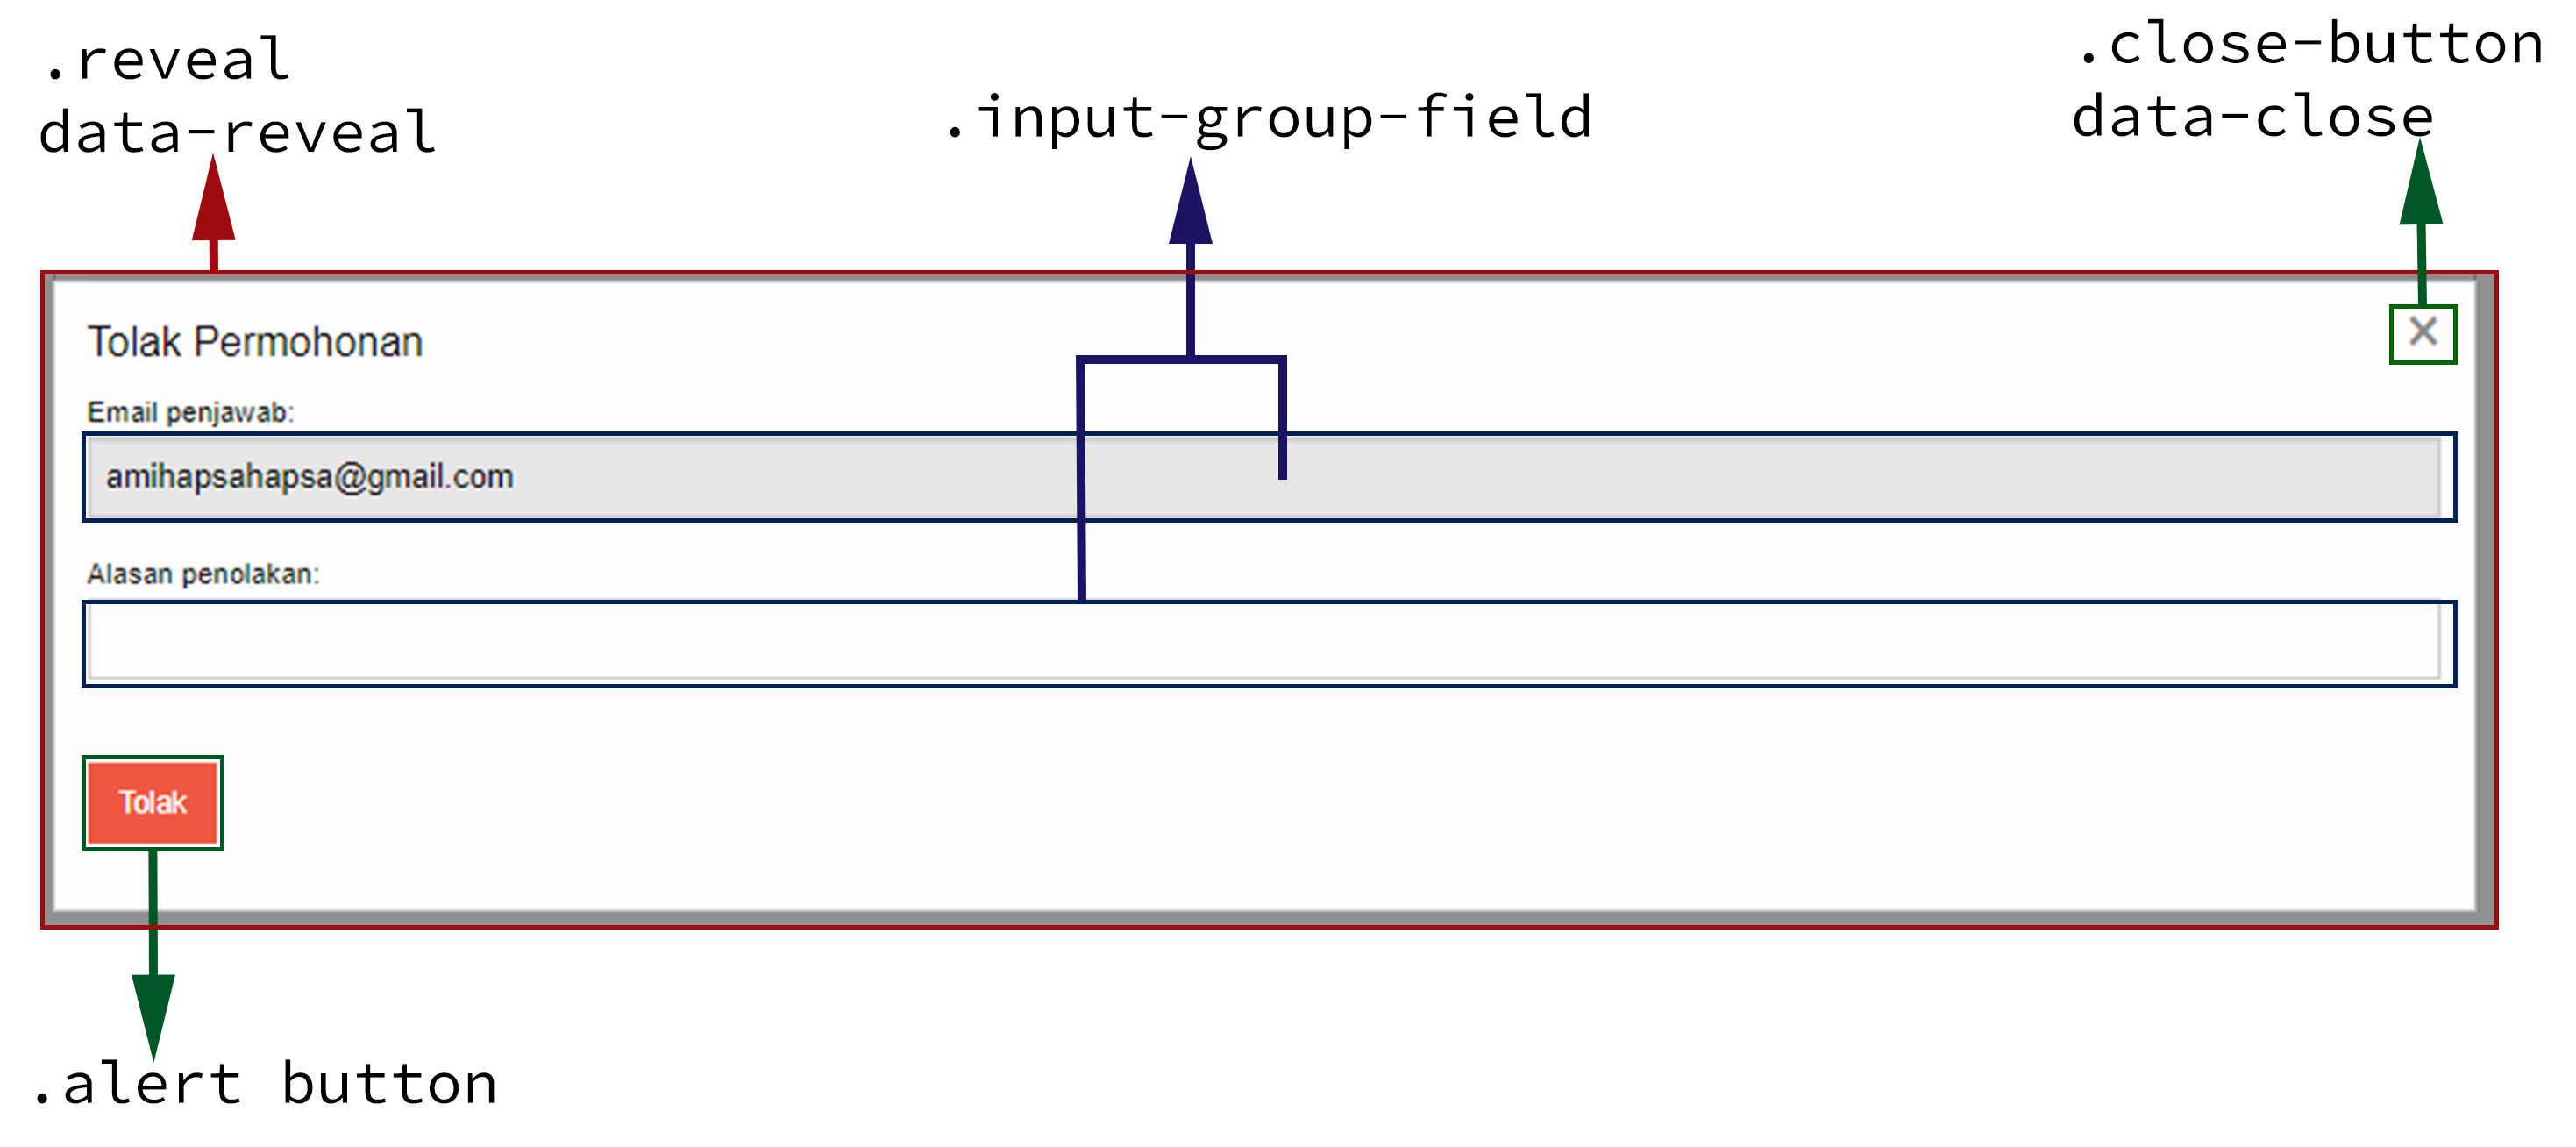
\includegraphics[width=\textwidth,height=\textheight,keepaspectratio]{foundation/analisis_modal_dislike_manajemen_cetak_transkrip.png}
		\caption{Modal tolak.} 
	\end{subfigure}
	\begin{subfigure}[b]{0.45\linewidth} 
		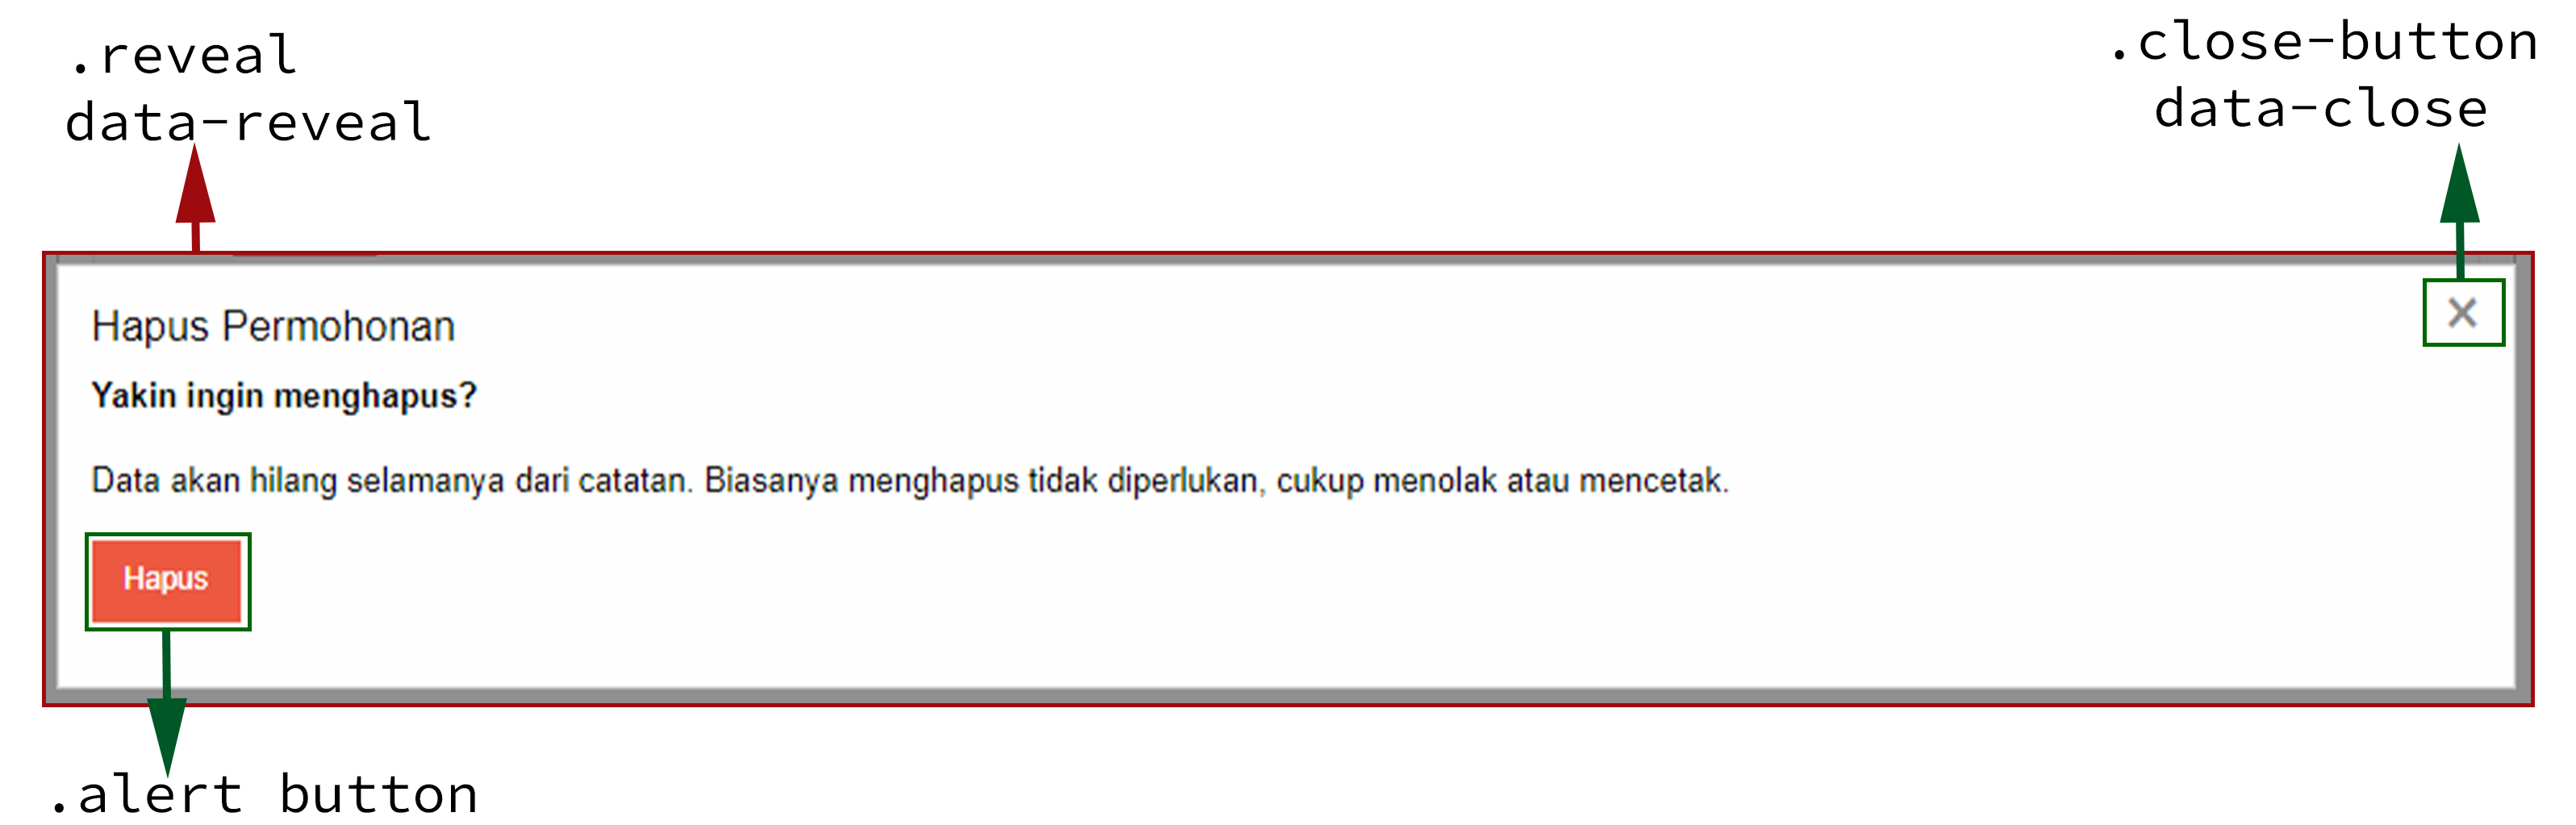
\includegraphics[width=\textwidth,height=\textheight,keepaspectratio]{foundation/analisis_modal_trash_manajemen_cetak_transkrip.png}
		\caption{Modal hapus.}
	\end{subfigure}
	\caption{Analisis modal pada halaman manajemen cetak transkrip.}
	\label{fig:analisisModalManajemenCetakTranskrip}	
\end{figure}

\noindent Kelas yang digunakan untuk seluruh modal tertera pada tabel ~\ref{table:analisisModalManajemenCetakTranskrip}.

\begin{table}[H]
	\centering
	\caption{Penggunaan kelas pada komponen modal manajemen cetak transkrip.}
	\begin{tabularx}{\textwidth}{lX}
		\toprule
		Kelas     & Penggunaan \\
		\midrule
		\texttt{.reveal data-reveal} & Kelas dan atribut untuk membuat komponen modal.\\
		\texttt{.close-button}  & Memungkinkan user untuk menutup modal yang telah terbuka.\\
		\texttt{data-close} & \\
		\texttt{aria-label} & \\
		\texttt{.stack} & Membuat tabel dalam modal lihat cetak transkrip.\\
		\texttt{.button} & Tombol "Sudah dicetak" berwarna biru untuk mengirimkan status permintaan sudah dicetak. \\
		\texttt{.alert button} & Tombol "Tolak" dan "Hapus" berwarna merah untuk menolak dan menghapus permintaan transkrip\\
		\texttt{.input-group-field} & Membuat  \textit{form} pada kolom "Email Penjawab" dan "Alasan Penolakan" pada modal hapus permintaan traskrip.\\
		\bottomrule
	\end{tabularx}%
	\label{table:analisisModalManajemenCetakTranskrip}
\end{table}%

\subsection{Halaman Permintaan Perubahan Kuliah}
Halaman permintaan perubahan kuliah terdiri dari dua konten: "Permohonan Baru" dan "Histori Permohonan" tertera pada gambar ~\ref{fig:analisisPermintaanPerubahanKuliah}. 

\subsubsection{Halaman Utama}
Setiap konten dipisahkan oleh border dalam Foundation disebut \texttt{callout}. Pada "Permohonan Baru" terdapat sebuah form yang berisi field-fiel dengan lebar yang berbeda - beda dan dikelompokan pada beberapa baris. Terdapat tiga tombol yaitu tombol biru "Kirim Permohonan" dan tombol abu-abu "Tambah pertemuan Ektra" .
Konten "Histori Permohonan" berisi tabel bergaris yang menampilkan data histori permohonan. 
\begin{figure} [H]
	\centering  
	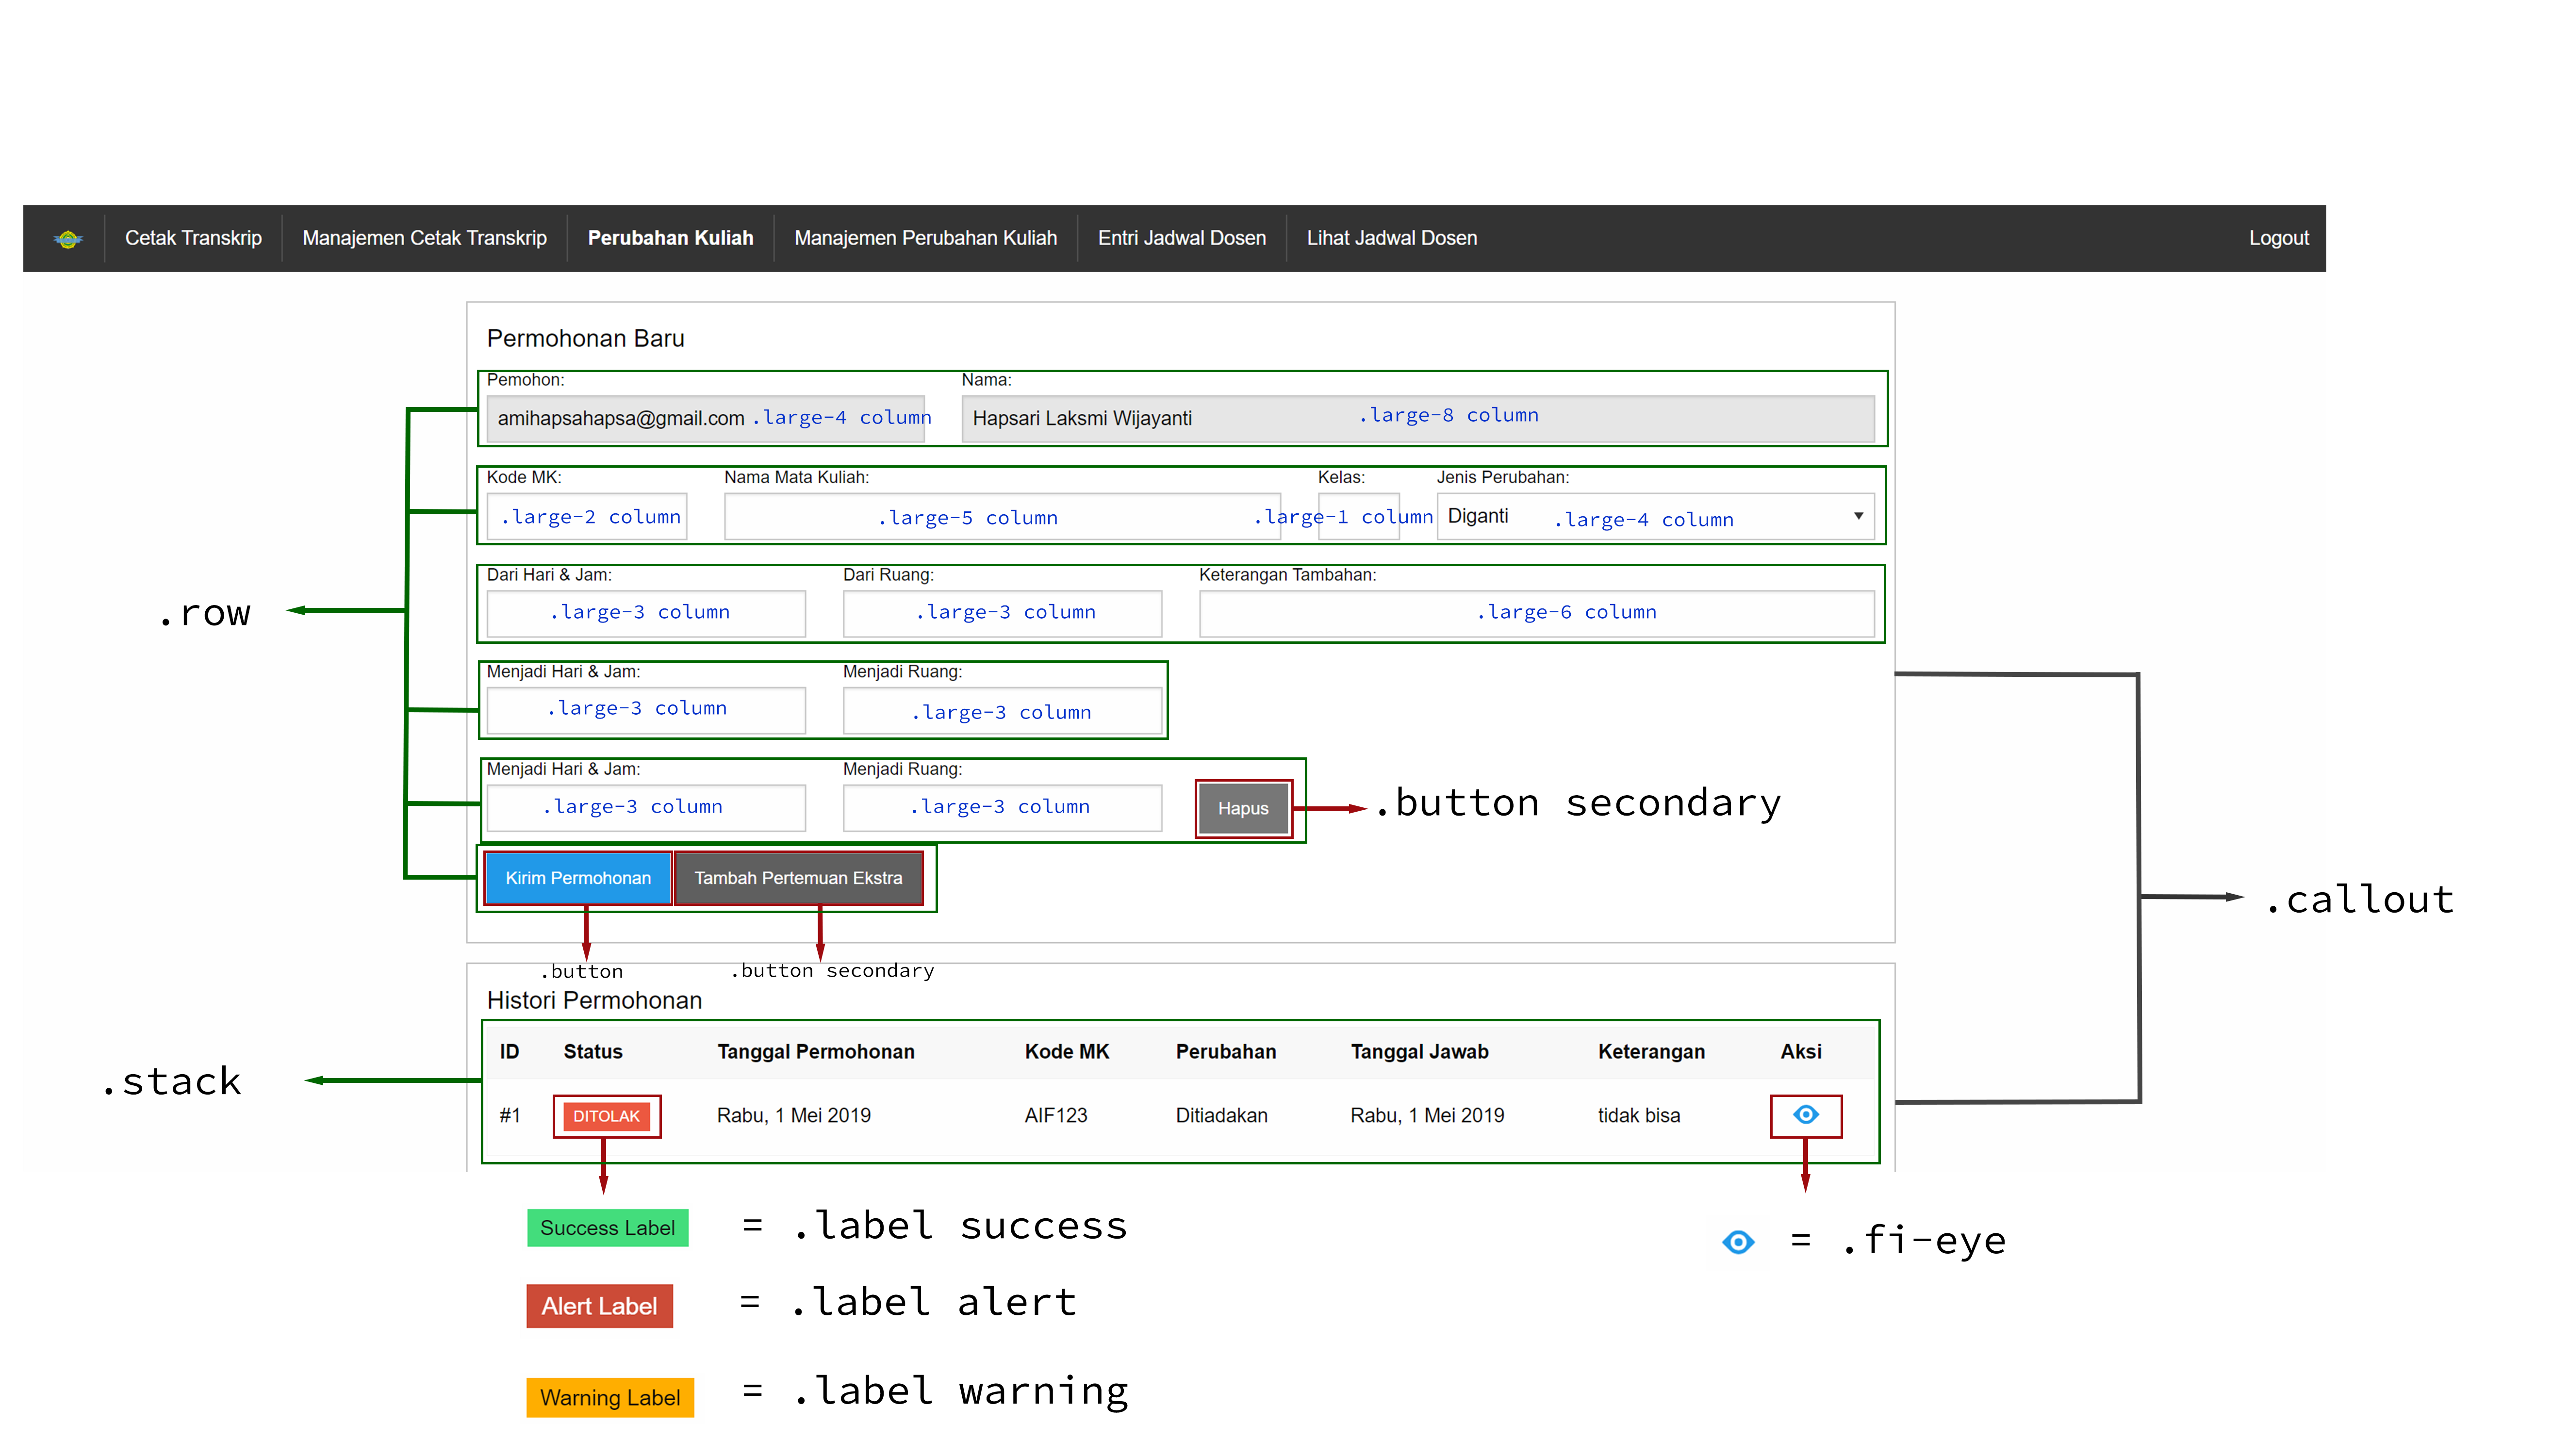
\includegraphics[width=\textwidth,height=\textheight,keepaspectratio]{foundation/analisis_perubahan_kuliah_request.png}
	\caption{Analisis halaman permintaan perubahan kuliah.}
	\label{fig:analisisPermintaanPerubahanKuliah}
\end{figure}

Penjelasan detil mengenai kelas - kelas dari gambar diatas terdapat pada tabel ~\ref{table:analisisPermintaanPerubahanKuliah} 
\begin{table}[H]
	\centering
	\caption{Penggunaan kelas pada halaman permintaan perubahan kuliah.}
	\begin{tabularx}{\textwidth}{lX}
		\toprule
		Kelas     & Penggunaan \\
		\midrule
		 \texttt{.row} & Kelas ini memiliki dua fungsi sebagai container konten dan mengatur beberapa \textit{field-form} menjadi satu baris. \\
		 \texttt{.large-* column} & Mendefinisikan lebar grid untuk masing - masing \textit{field} pada \textit{form}. \\
		 \texttt{.callout} & Untuk membuat border yang memisahkan konten permohonan baru dan histori permohonan.\\
		 \texttt{.stack} & Jenis tabel yang digunakan tabel histori permohonan, sehingga pada layar medium tabel akan tersusun secara bertumpuk.\\
		 \texttt{.fi-eye, data-open} & Ikon untuk menuju modal lihat detail permohonan berdasarkan ID.\\
		\bottomrule
	\end{tabularx}%	
	\label{table:analisisPermintaanPerubahanKuliah}
\end{table}

Pada tabel ~\ref{table:analisisLabelPermintaanPerubahanKuliah} kolom 'Status' mendefinisikan hasil permohonan perubahan kuliah, tiga jenis status menggunakan tiga jenis kelas yang berbeda-beda yaitu:\\

\begin{table}[H]
	\centering
	\caption{Penggunaan komponen label pada kolom status histori permohonan.}
	\begin{tabularx}{\textwidth}{lX}
		\toprule
		Kelas     & Penggunaan \\
		\midrule
		 \texttt{.label success} & Label untuk perubahan kuliah berhasil.\\
		 \texttt{.label alert} & Label untuk perubahan kuliah gagal.\\
		 \texttt{.label warning} & Label untuk perubahan kuliah diproses.\\
		\bottomrule
	\end{tabularx}%
	\label{table:analisisLabelPermintaanPerubahanKuliah}
\end{table}

\subsubsection{Modal: Lihat}
Kolom 'Aksi' berisi ikon mata yang akan mereferensikan ke modal lihat pada data permohonan perubahan kuliah. Modal lihat tertera pada gambar ~\ref{fig:analisisModalPermintaanPerubahanKuliah}:\\
\begin{figure}[H]
	\centering  
	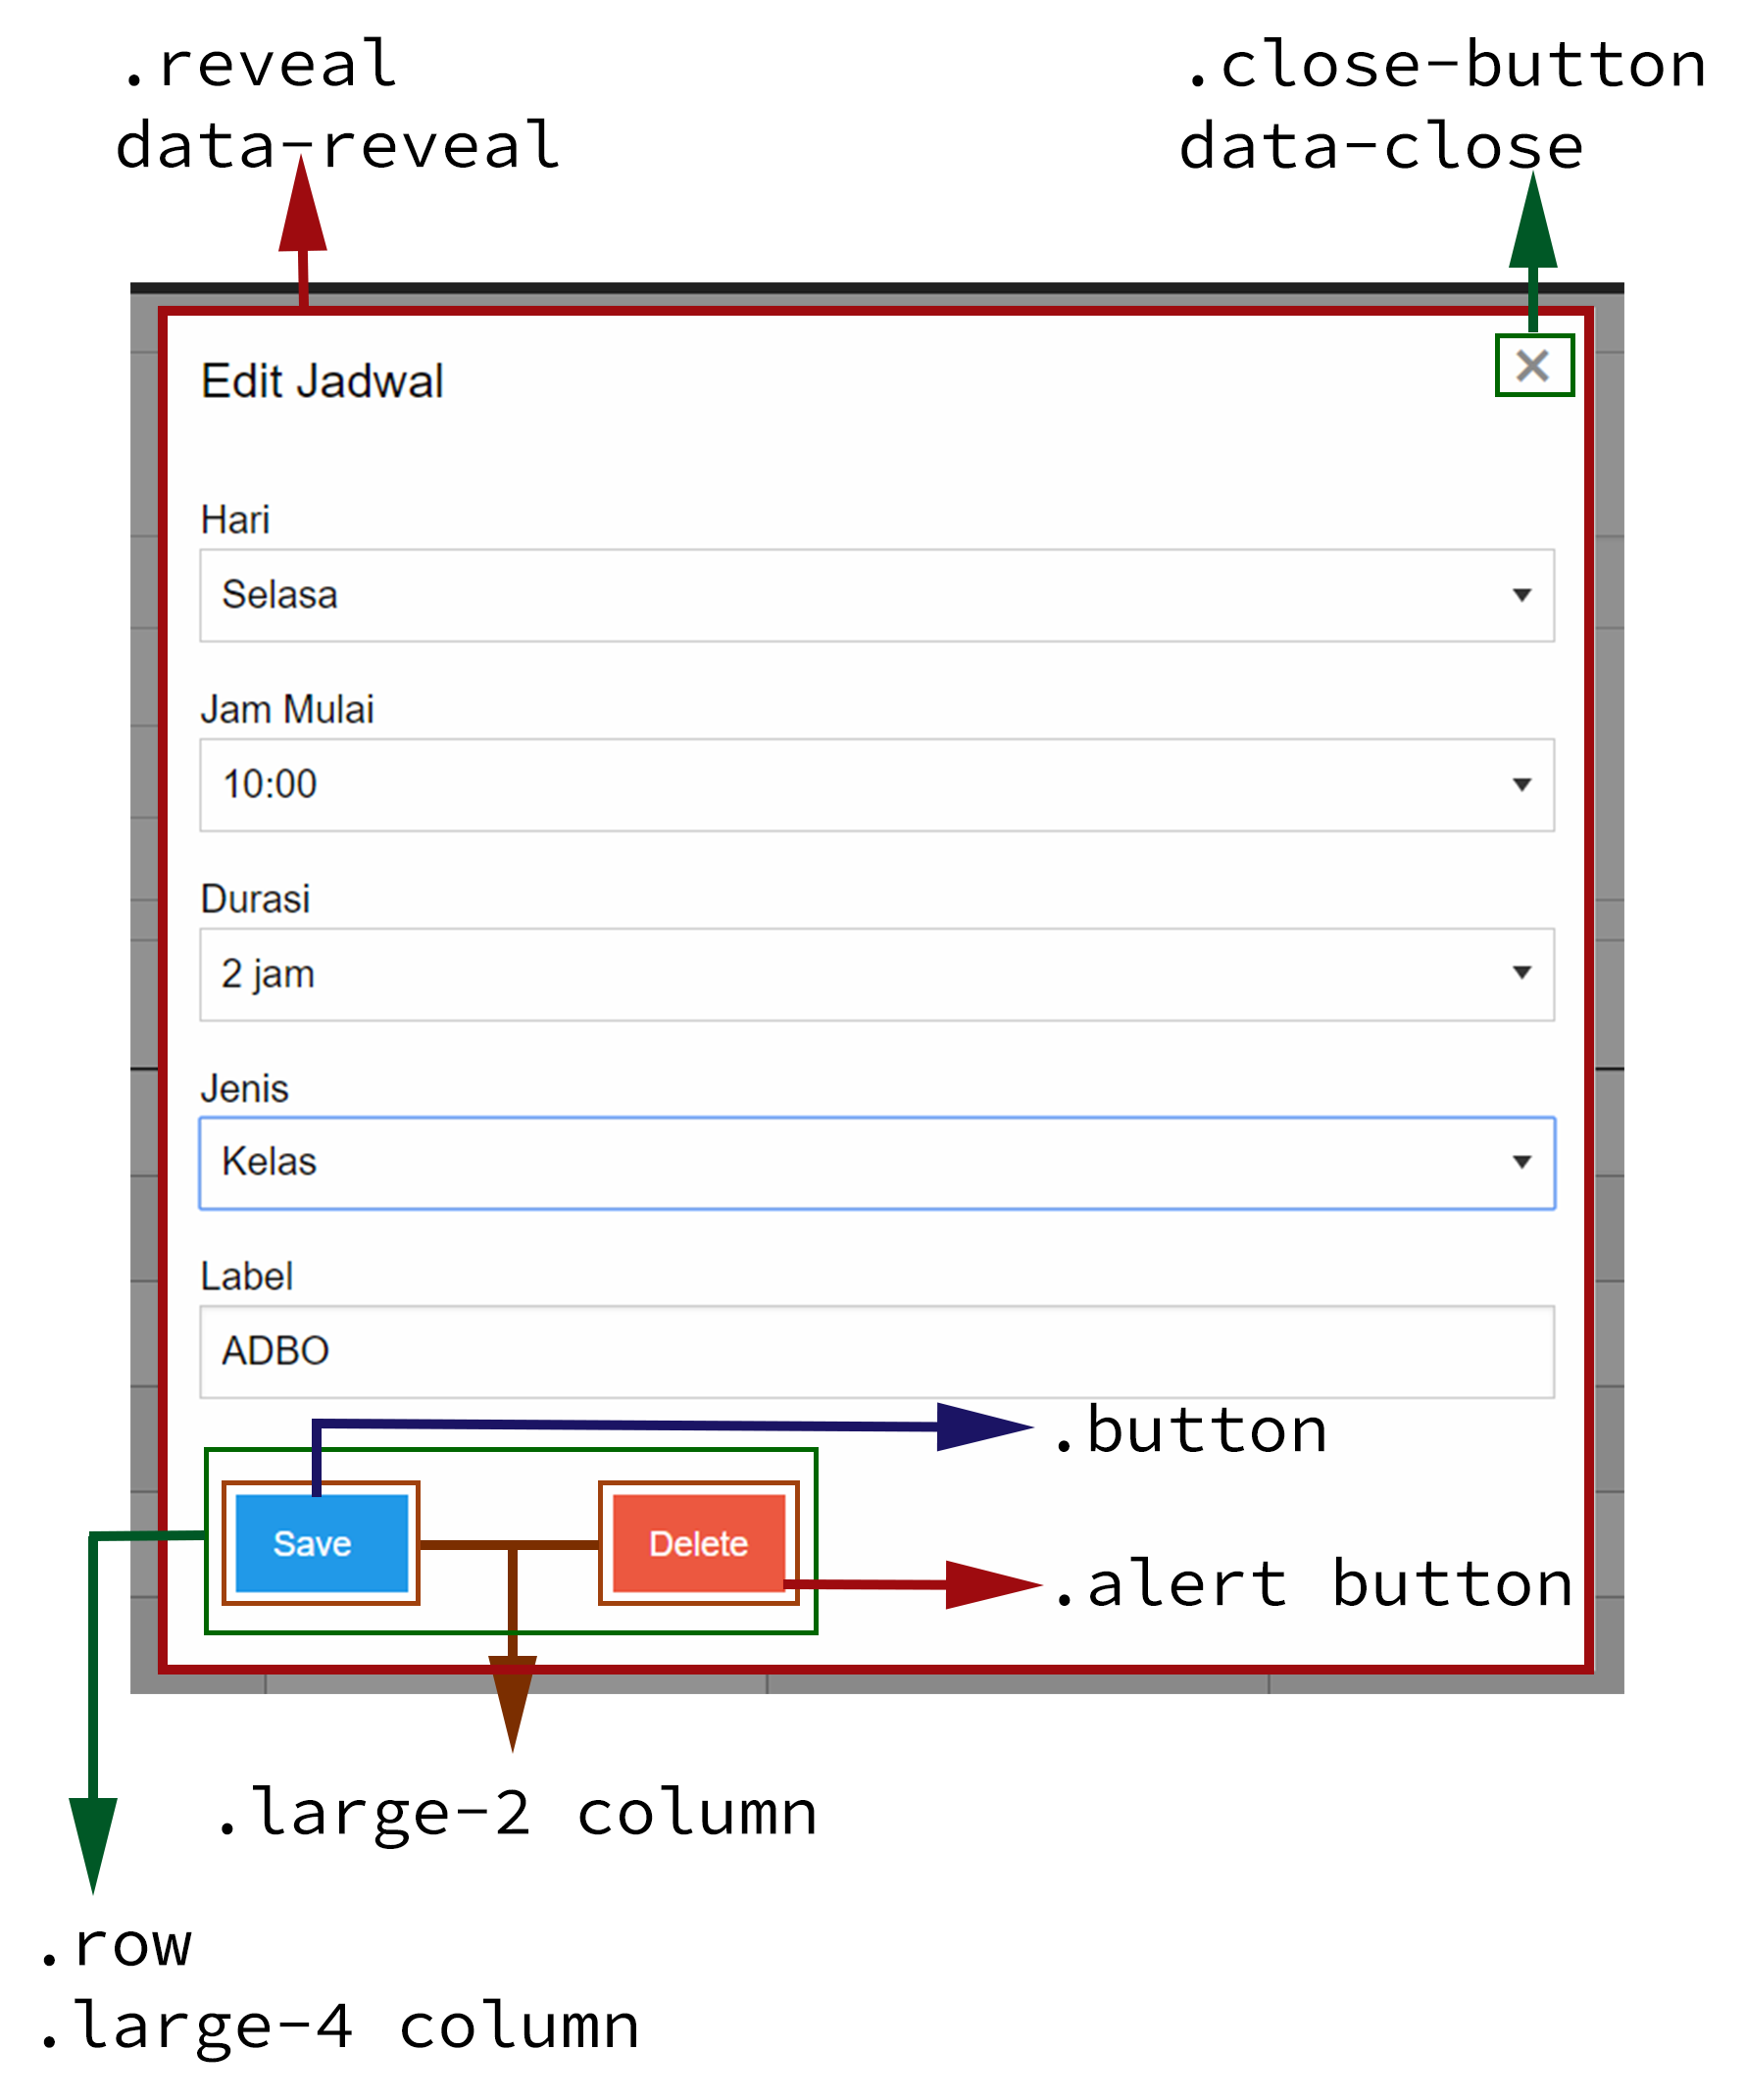
\includegraphics[width=0.6\textwidth,height=\textheight,keepaspectratio]{foundation/analisis_modal_eye_perubahan_kuliah_request.png}
	\caption{Analisis modal lihat.}
	\label{fig:analisisModalPermintaanPerubahanKuliah}
\end{figure}

\noindent Kelas yang digunakan dalam modal ditampilkan pada tabel ~\ref{table:analisisModalPermintaanPerubahanKuliah}.\\
\begin{table}[H]
	\centering
	\caption{Penggunaan kelas komponen modal lihat permintaan perubahan kuliah.}
	\begin{tabularx}{\textwidth}{lX}
		\toprule
		Kelas     & Penggunaan \\
		\midrule
		 \texttt{.reveal data-reveal} & Membuat modal yang menampung tabel detail permohonan.\\
		 \texttt{.close-button data-close aria-label} & Menutup modal yang telah terbuka dengan memberikan label `x' pada tombol.\\
		 \texttt{.stack} &	Membuat tabel detail permohonan perubahan kuliah.\\
		\bottomrule
	\end{tabularx}%	
	\label{table:analisisModalPermintaanPerubahanKuliah}
\end{table}

\subsection{Halaman Manajemen Perubahan Kuliah}
Halaman pada gambar ~\ref{fig:analisisManajemenPerubahanKuliah} menampilkan data permohonan perubahan kuliah berisi sebuah tabel dimana pada kolom 'Status' menggunakan kelas \texttt{.callout} untuk \textit{highlight} status dan pada kolom 'Aksi' menampilkan lima jenis ikon dari \textit{Library} Font Awesome. Setiap ikon merupakan link menuju modal.
\subsubsection{Halaman Utama}
\begin{figure} [H]
	\centering  
	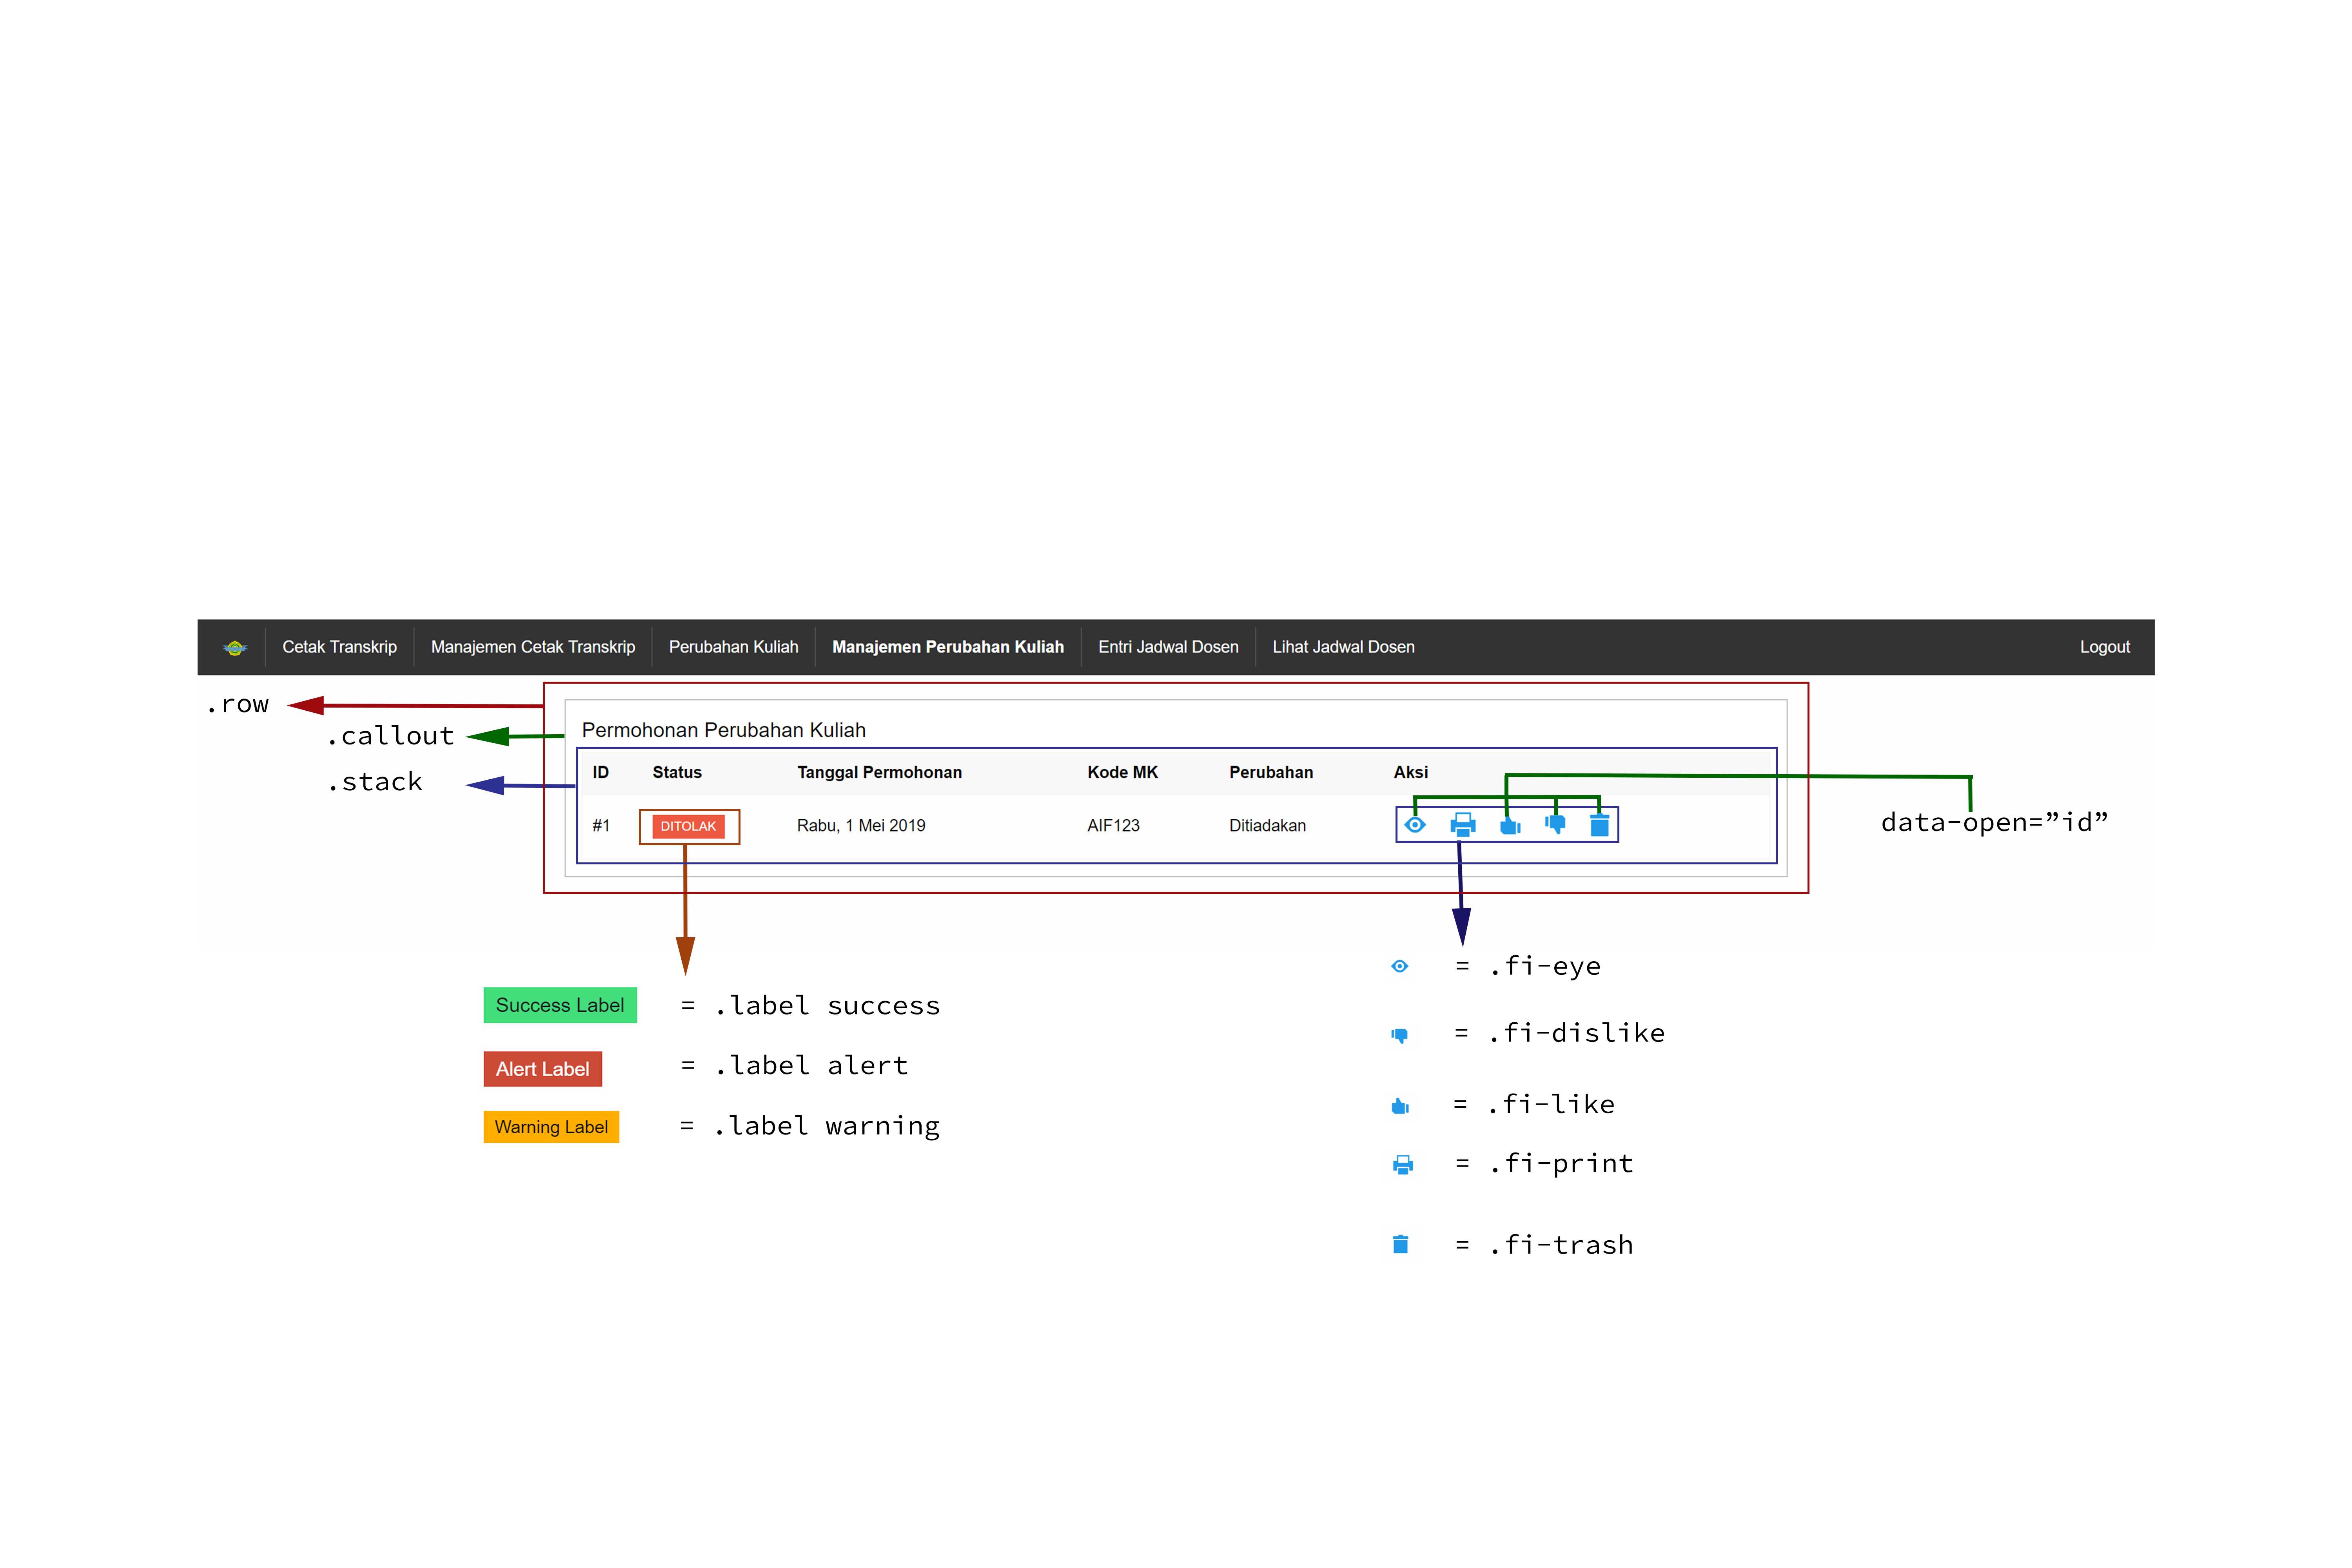
\includegraphics[width=\textwidth,height=\textheight,keepaspectratio]{foundation/analisis_manajemen_perubahan_kuliah.png}
	\caption{Analisis halaman manajemen perubahan kuliah.}
	\label{fig:analisisManajemenPerubahanKuliah}
\end{figure}
Kelas - kelas yang digunakan pada gambar diatas tertera pada tabel ~\ref{table:analisisManajemenPerubahanKuliah}:
\begin{table}[H]
	\centering
	\caption{Penggunaan kelas pada halaman manajemen perubahan kuliah.}
	\begin{tabularx}{\textwidth}{lX}
		\toprule
		Kelas     & Penggunaan \\
		\midrule
		\texttt{.row} & Kelas ini memiliki dua fungsi sebagai container konten dan mengatur beberapa \textit{field-form} menjadi satu baris.\\ 
		\texttt{.callout} & Untuk membuat border yang memisahkan konten permohonan baru dan histori permohonan.\\
		\texttt{.stack} & Jenis tabel yang digunakan tabel histori permohonan, sehingga pada layar medium tabel akan tersusun secara bertumpuk.\\
		\bottomrule
	\end{tabularx}%	
	\label{table:analisisManajemenPerubahanKuliah}
\end{table}

\noindent Pada kolom 'Status' kelas yang digunakan dari komponen \texttt{callout} tertera pada tabel ~\ref{table:analisisLabelManajemenPerubahanKuliah}.
\begin{table}[H]
	\centering
	\caption{Penggunaan komponen label pada kolom status permohonan perubahan kuliah.}
	\begin{tabularx}{\textwidth}{lX}
		\toprule
		Kelas     & Penggunaan \\
		\midrule
		\texttt{.label success} & Label untuk permitaan perubahan kuliah telah disetujui.\\
		\texttt{.label alert} &  Label untuk permitaan perubahan kuliah telah ditolak.\\
		\texttt{.label warning} & Label untuk permintaan perubahan kuliah sedang diproses.\\
		\bottomrule
	\end{tabularx}%	
	\label{table:analisisLabelManajemenPerubahanKuliah}
\end{table}\\

\noindent Kemudian pada kolom 'Aksi' kelas yang digunakan dari \textit{library Font Awesome} tertera pada tabel ~\ref{table:analisisIkonManajemenPerubahanKuliah}.
\begin{table}[H]
	\centering
	\caption{Penggunaan ikon font awesome pada halaman manajemen perubahan kuliah.}
	\begin{tabularx}{\textwidth}{lX}
		\toprule
		Kelas     & Penggunaan \\
		\midrule
		\texttt{fi-eye} & Ikon menuju modal lihat permohonan perubahan kuliah.\\
		\texttt{fi-like} & Ikon menuju modal persetujuan permohonan perubahan kuliah.\\
		\texttt{fi-dislike} & Ikon menuju modal persetujuan penolakan perubahan kuliah.\\
		\texttt{fi-print} & Ikon untuk menuju halaman cetak jadwal perubahan kuliah.\\
		\texttt{fi-trash} & Ikon untuk menghapus permitaan perubahan kuliah.\\
		\bottomrule
	\end{tabularx}%	
	\label{table:analisisIkonManajemenPerubahanKuliah}
\end{table}

\subsubsection{Modal}
Apabila user memilih salah satu ikon dari kolom 'Aksi' maka modal akan muncul. Terdapat lima macam modal yaitu: modal lihat, modal setuju, modal tolak, modal print dan modal hapus perubahan kuliah. Berikut ini gambar ~\ref{fig:analisisModalManajemenPerubahanKuliah} modal yang ada pada halaman manajemen perubahan kuliah
\begin{figure} [H]	
	\centering
	\begin{subfigure}[b]{0.45\linewidth} 
		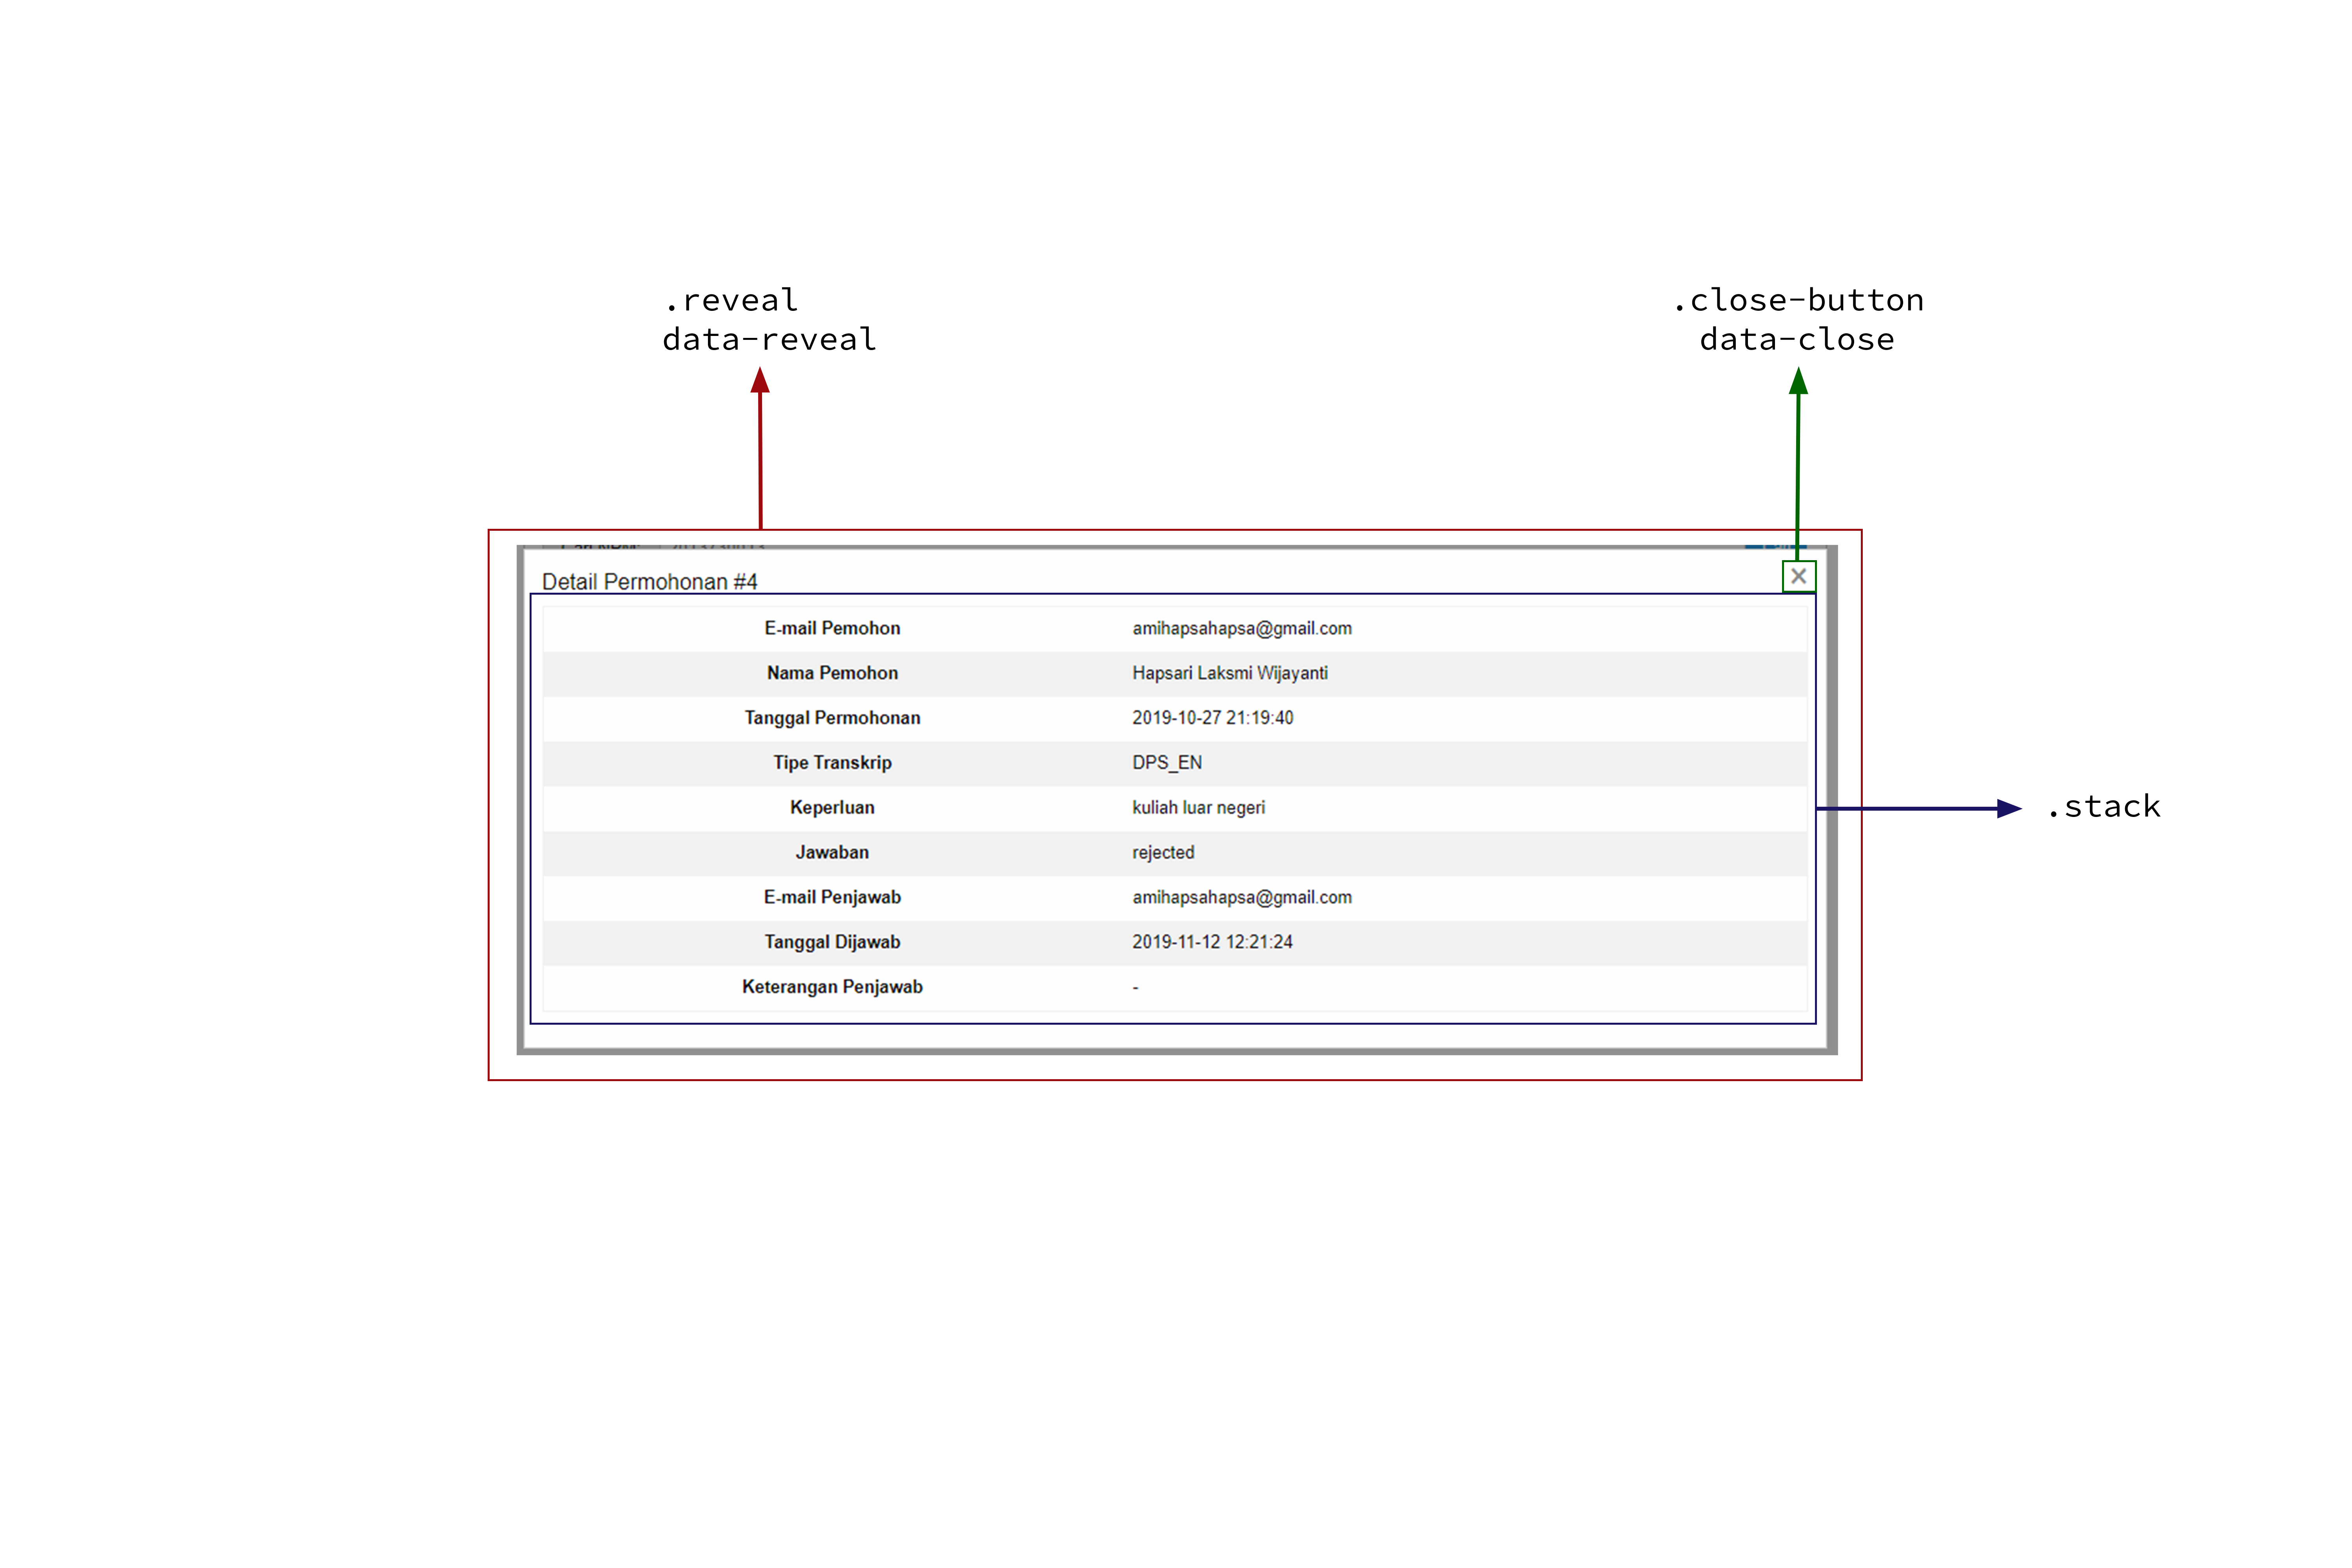
\includegraphics[width=\textwidth,height=\textheight,keepaspectratio]{foundation/analisis_modal_eye_manajemen_perubahan_kuliah.png}
		\caption{Modal lihat.}  
	\end{subfigure}	
	\begin{subfigure}[b]{0.3\linewidth}   
		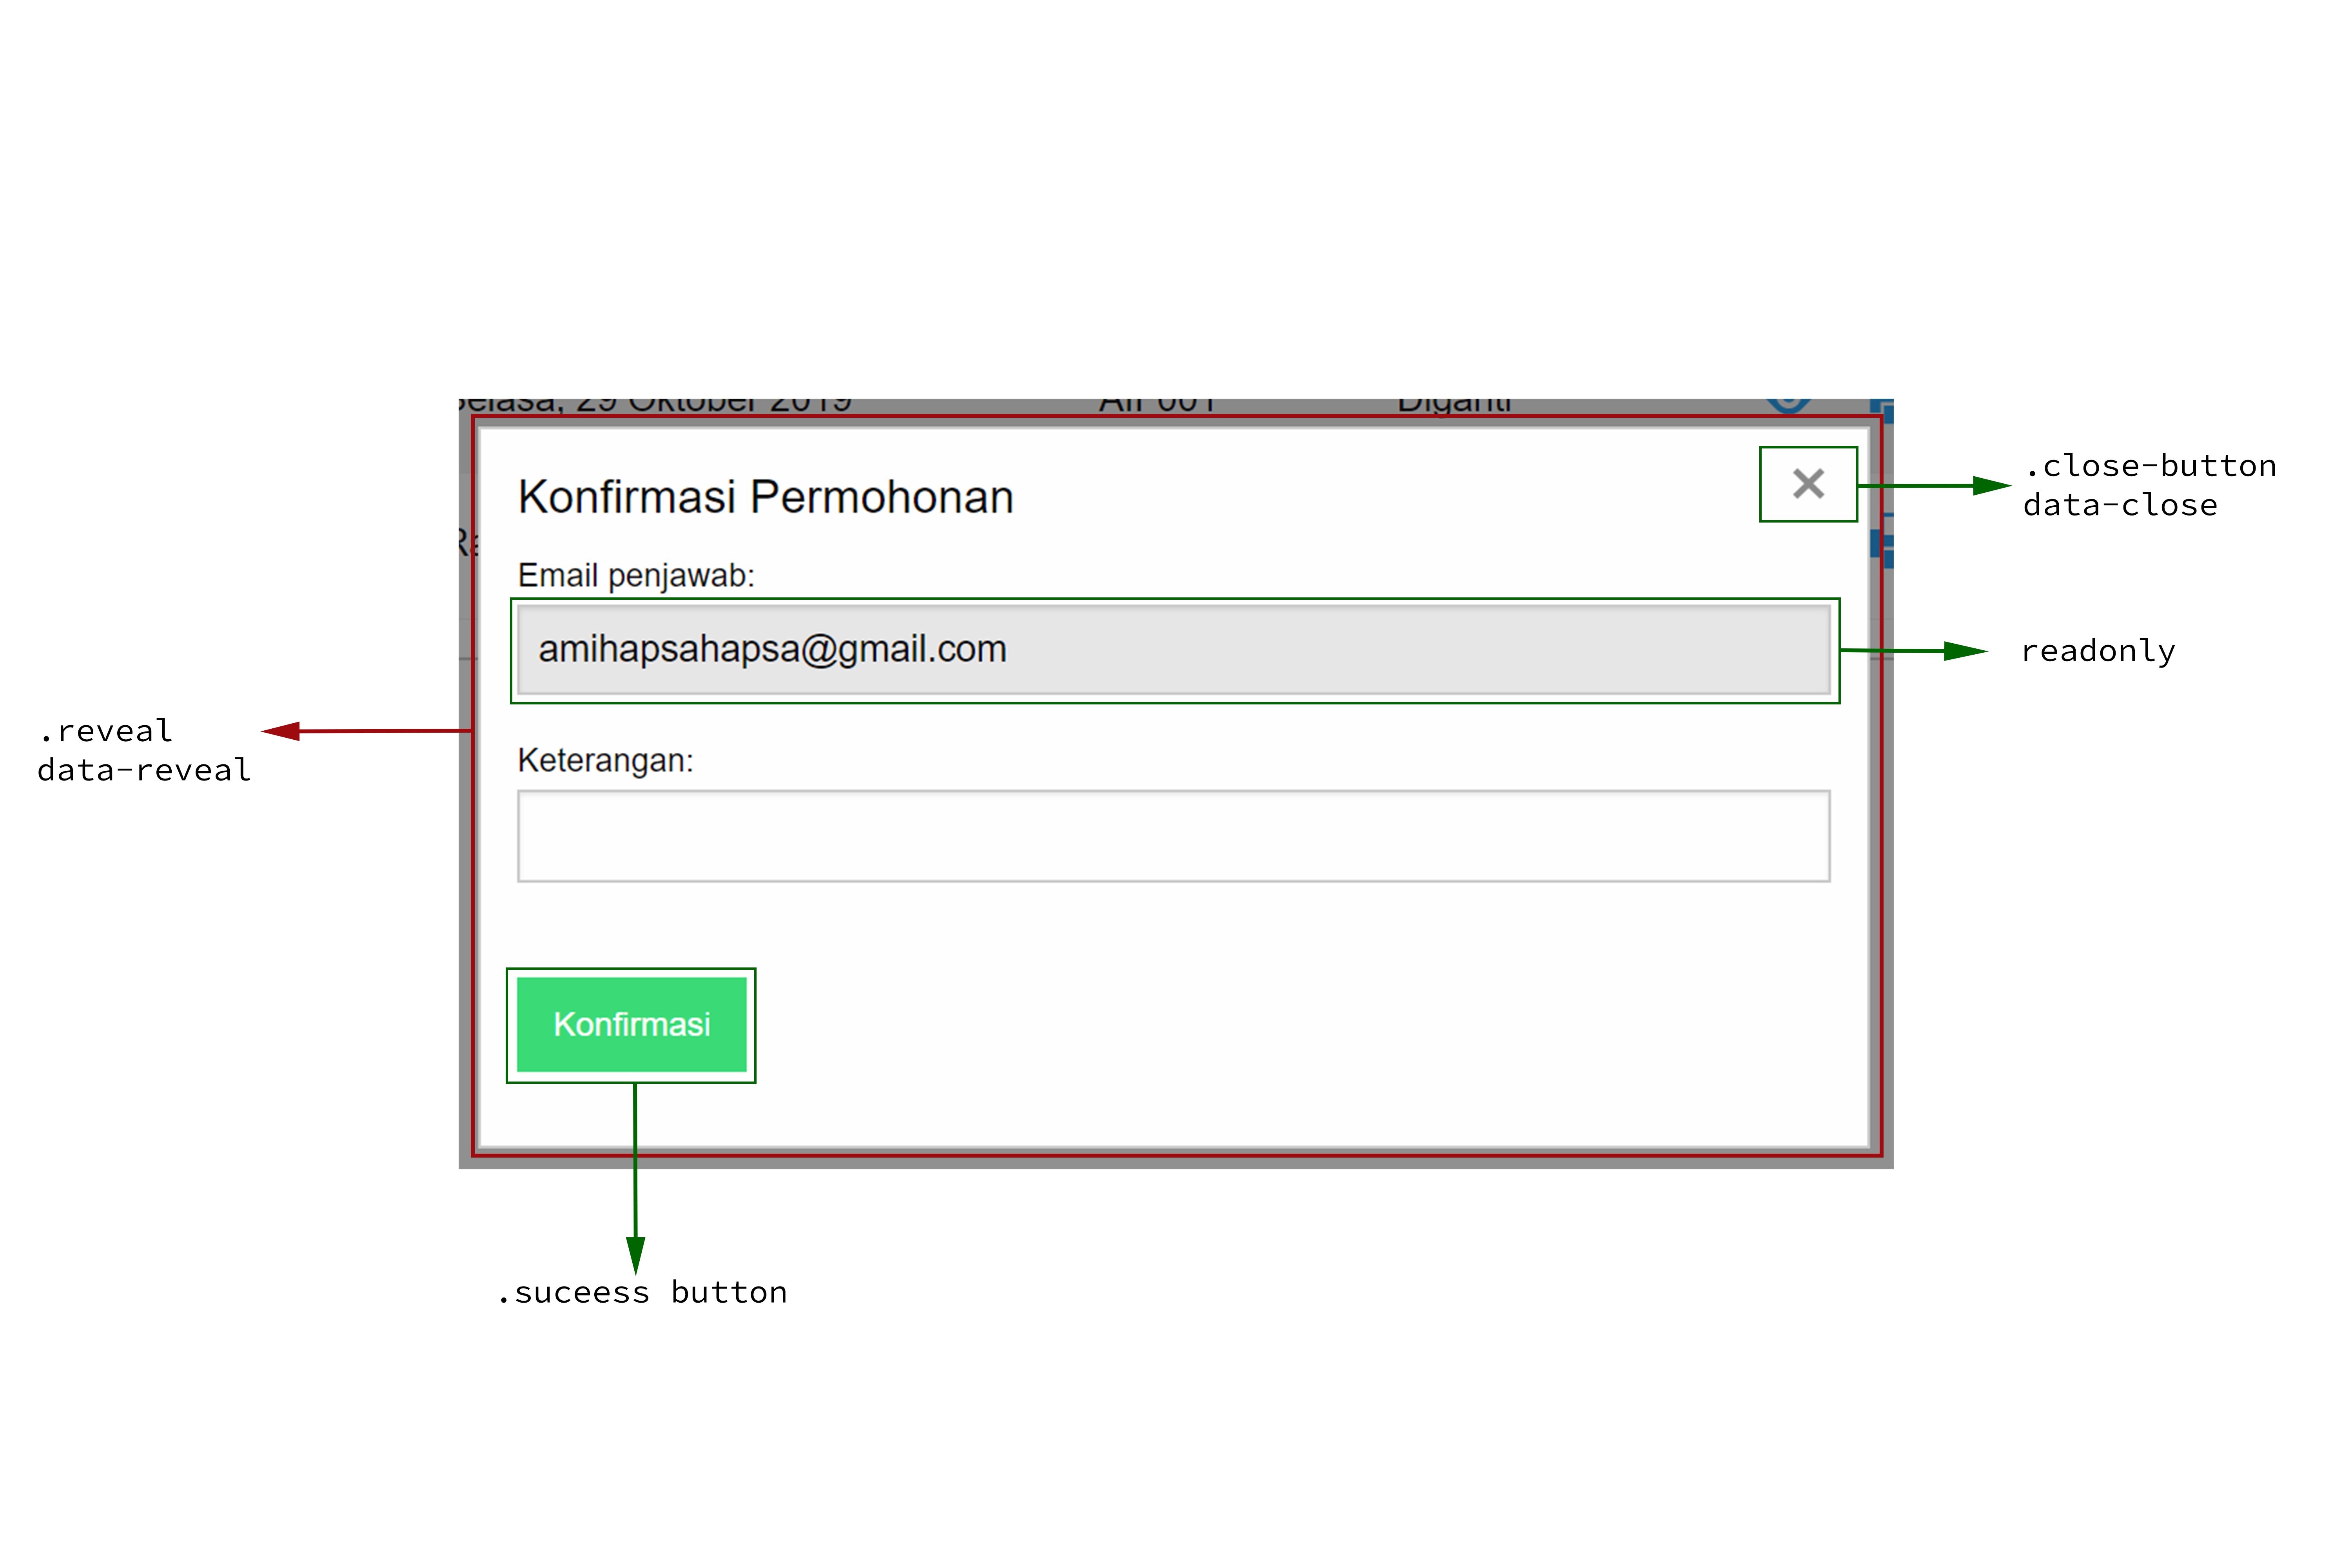
\includegraphics[width=\textwidth,height=\textheight,keepaspectratio]{foundation/analisis_modal_like_manajemen_perubahan_kuliah.png}
		\caption{Modal setuju.}
	\end{subfigure}
\end{figure}

\begin{figure} [H] 
	\centering
	\ContinuedFloat
	\begin{subfigure}[b]{0.6\linewidth}
		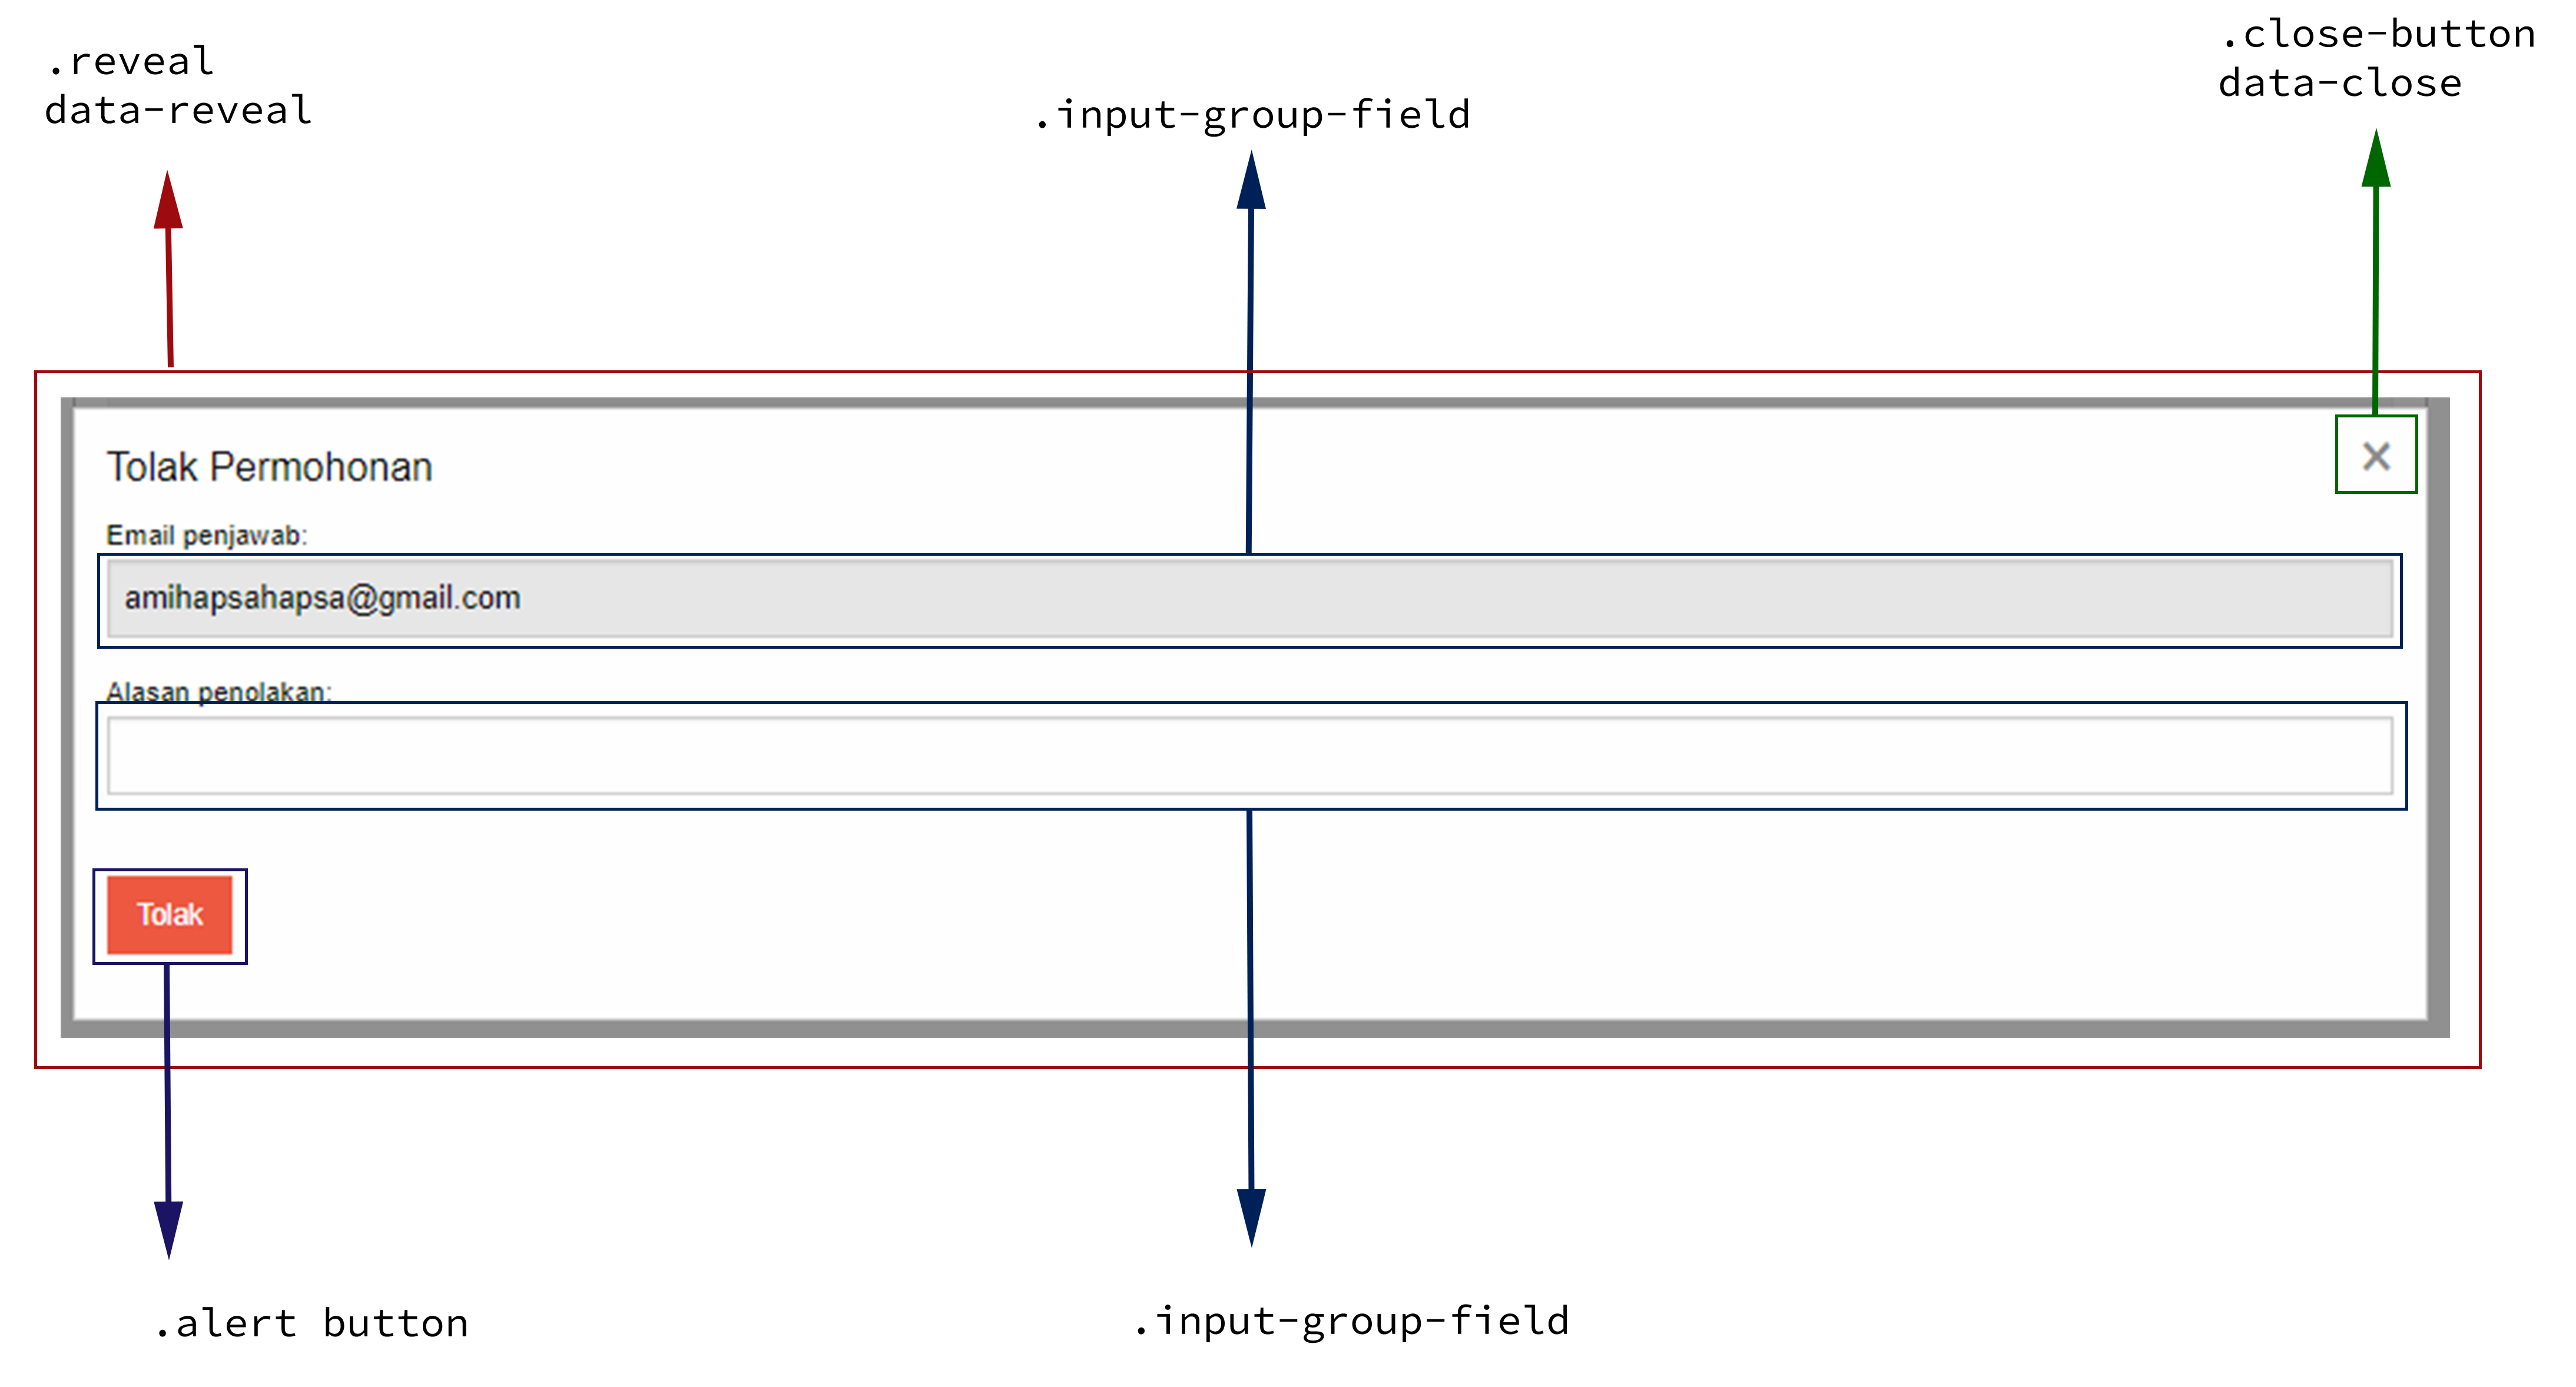
\includegraphics[width=\textwidth,height=\textheight,keepaspectratio]{foundation/analisis_modal_dislike_manajemen_perubahan_kuliah.png}
		\caption{Modal tolak.}  
	\end{subfigure}
\end{figure}

\begin{figure} [H] 
	\centering
	\ContinuedFloat
	\begin{subfigure}[b]{0.35\linewidth} 
		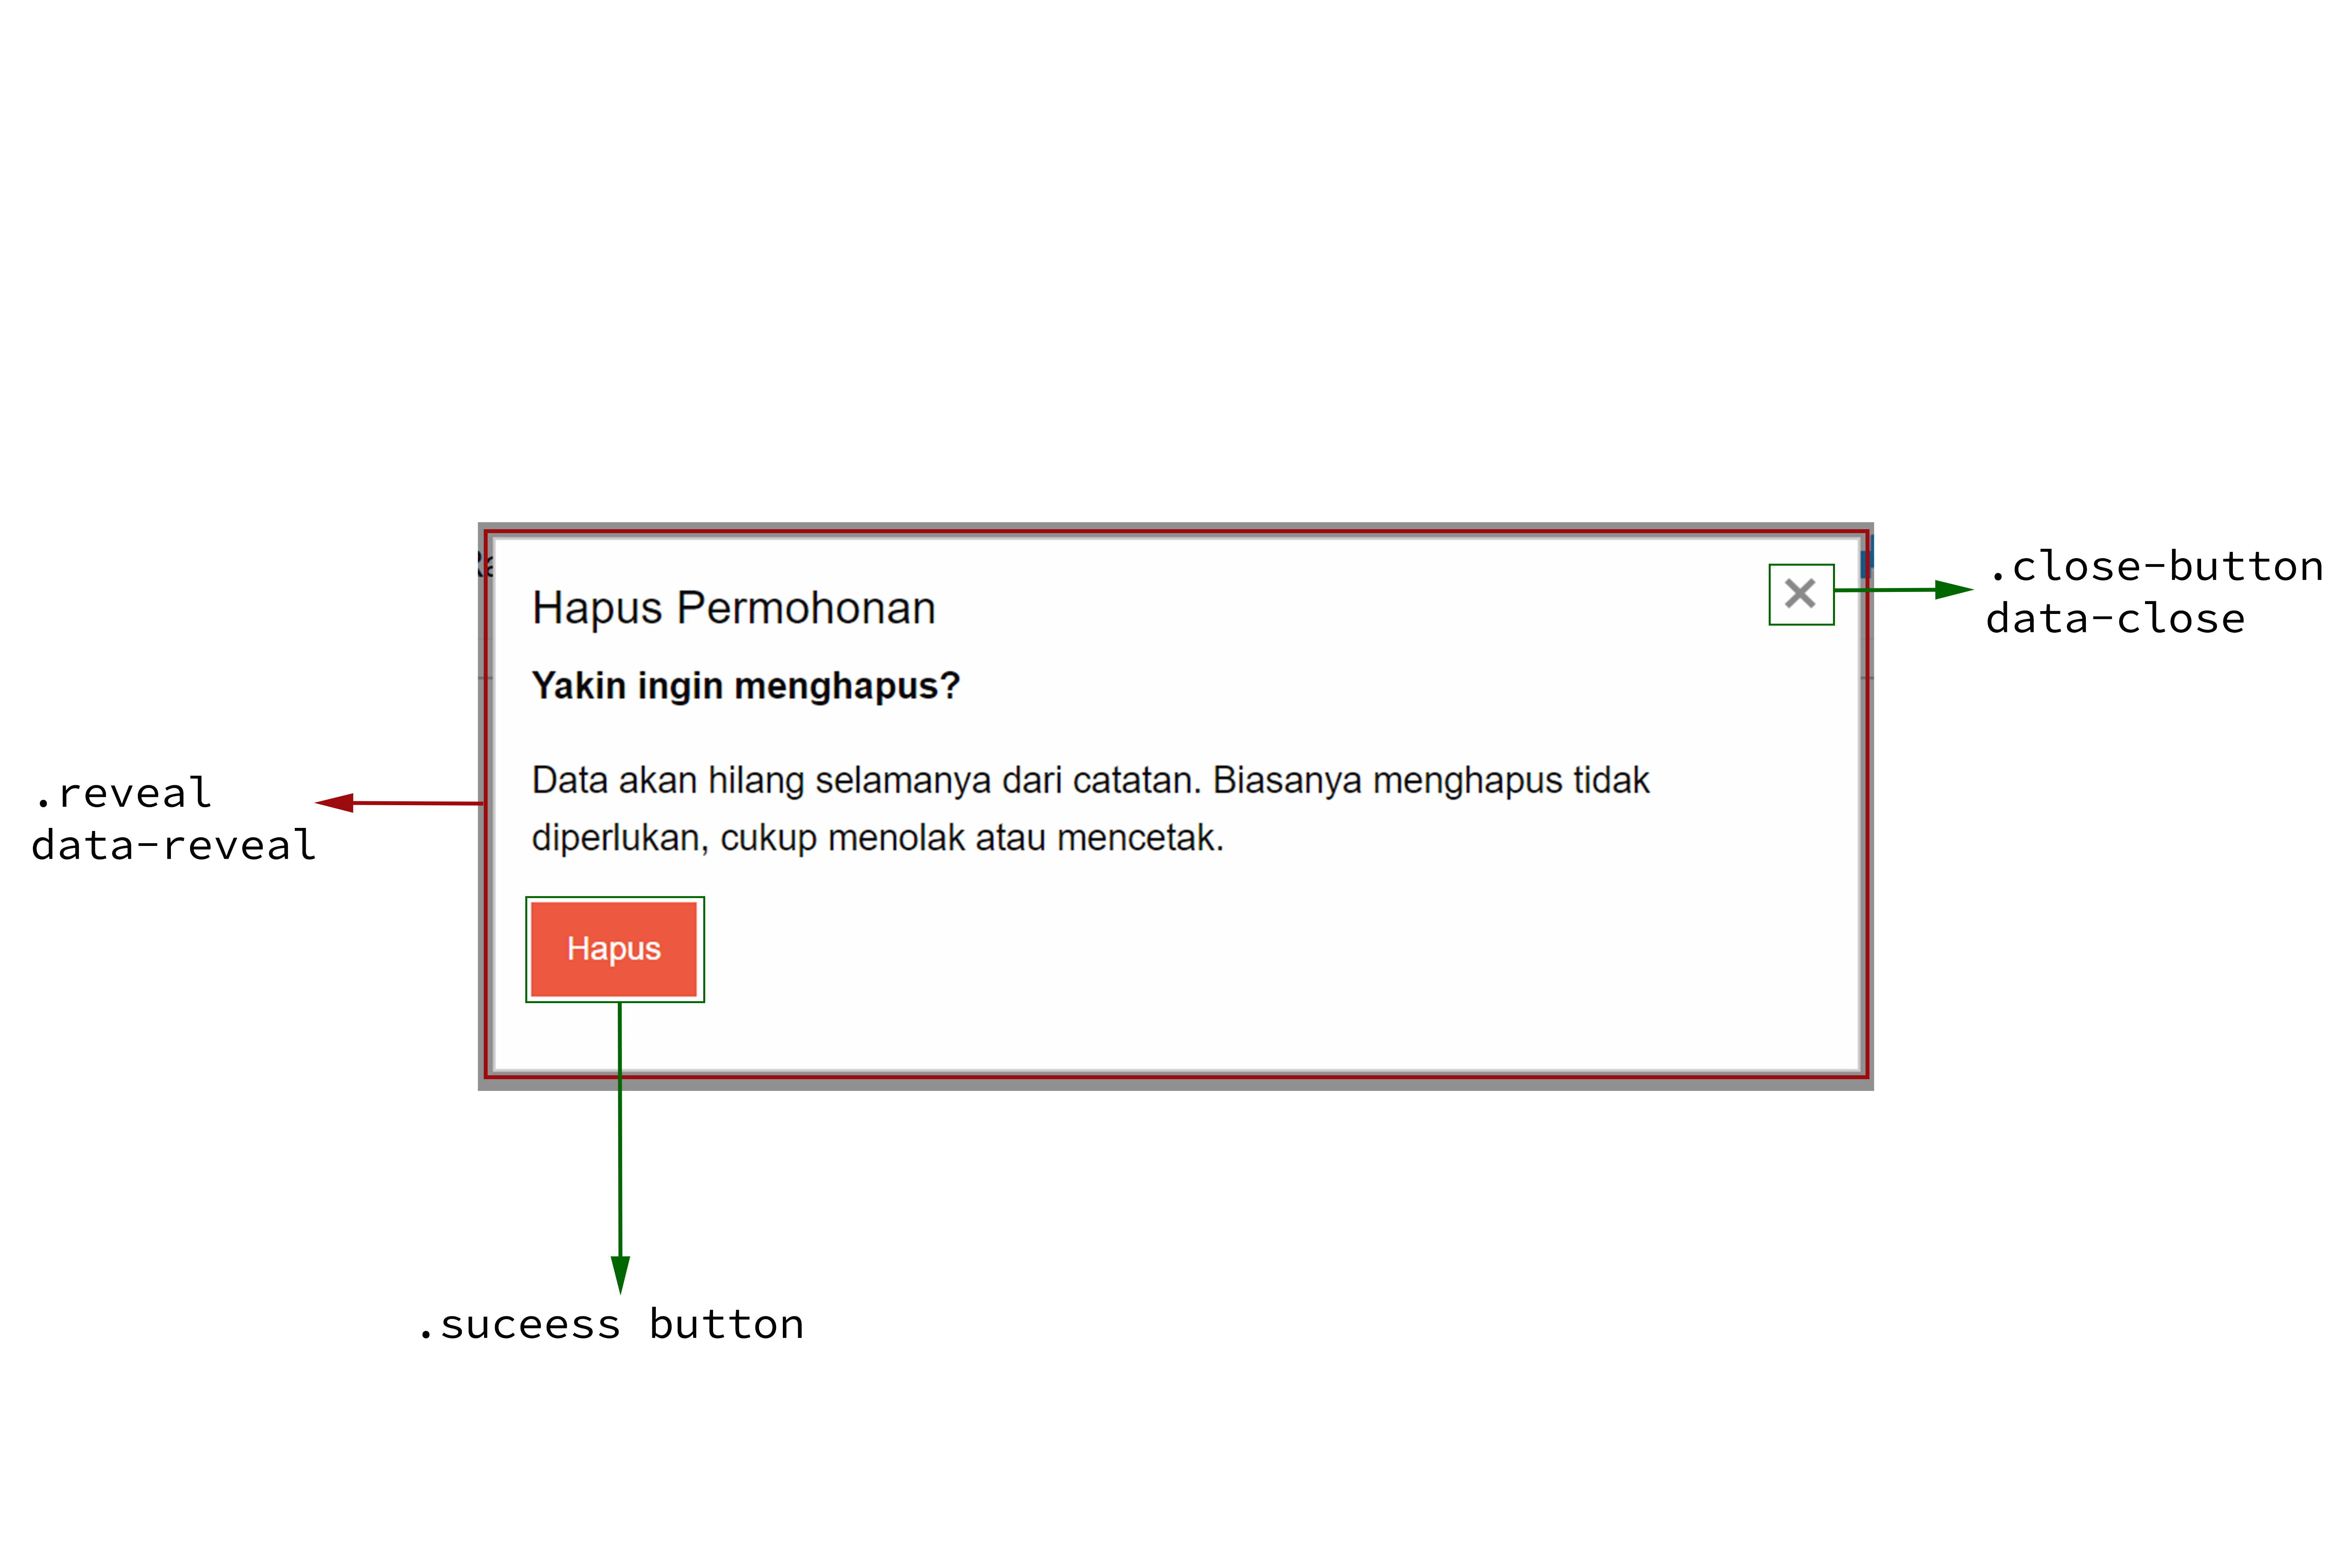
\includegraphics[width=\textwidth,height=\textheight,keepaspectratio]{foundation/analisis_modal_trash_manajemen_perubahan_kuliah.png}
		\caption{Modal hapus.}
	\end{subfigure}
	\begin{subfigure}[b]{0.55\linewidth}
		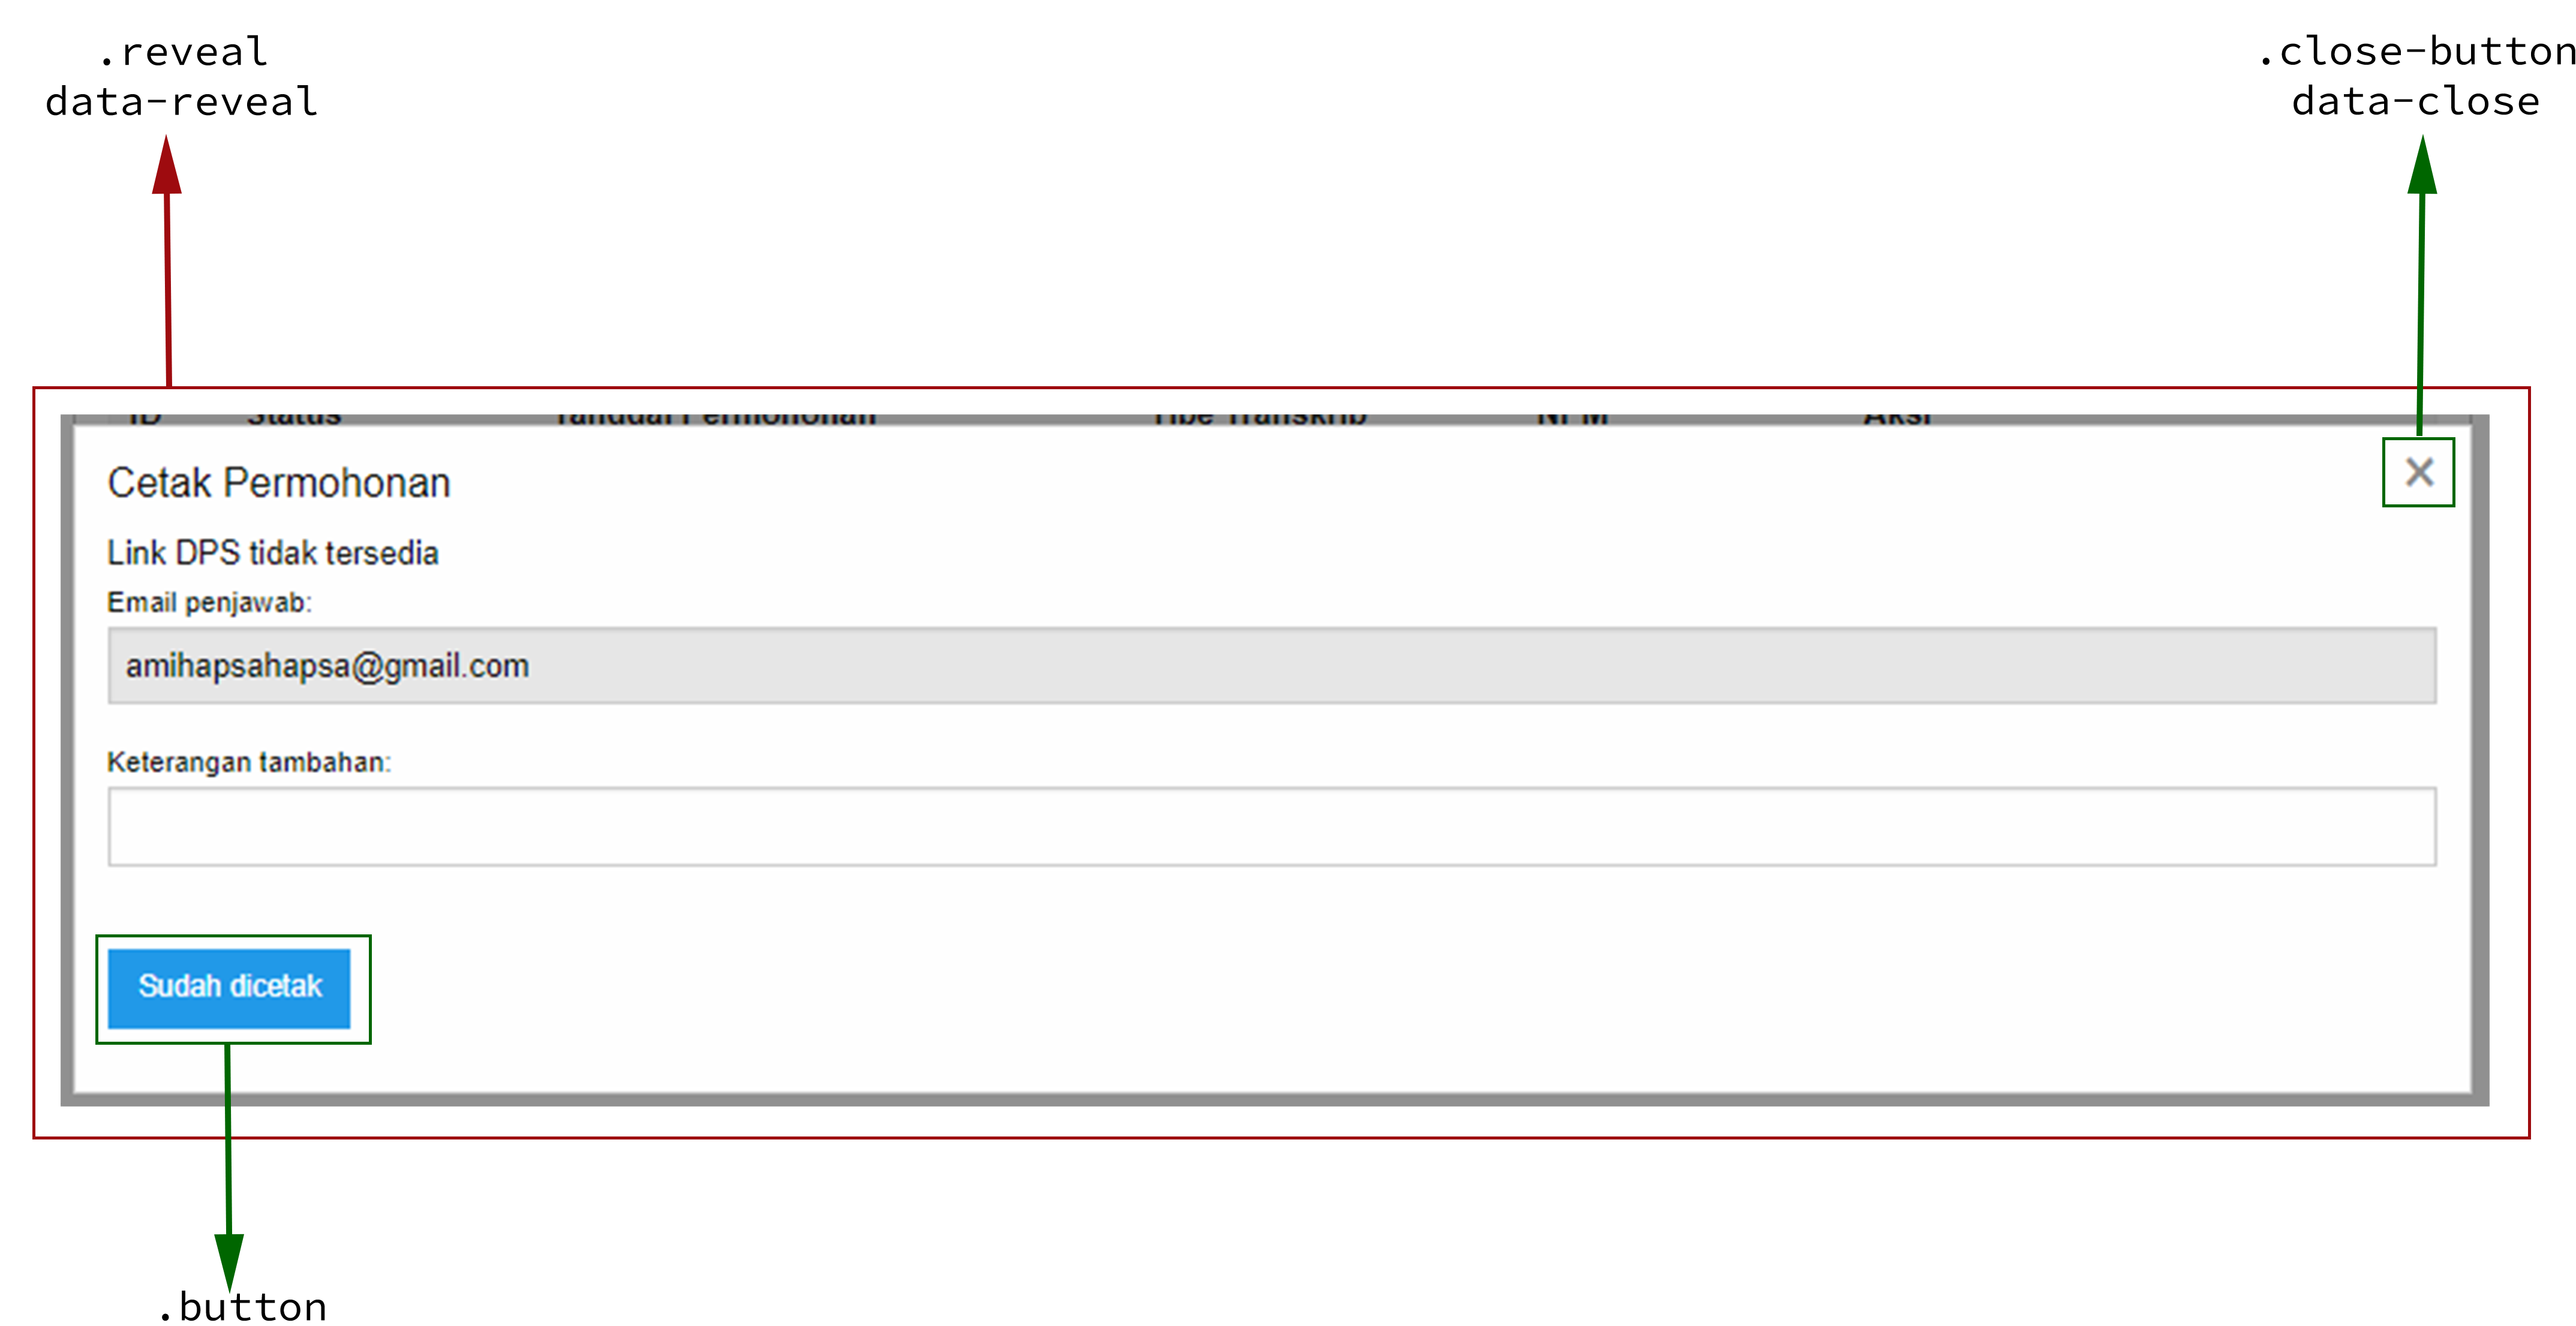
\includegraphics[width=\textwidth,height=\textheight,keepaspectratio]{foundation/analisis_modal_print_manajemen_cetak_transkrip.png}
		\caption{Modal print.}  
	\end{subfigure}	 
\caption{Analisis modal pada halaman manajemen perubahan kuliah.}
\label{fig:analisisModalManajemenPerubahanKuliah}
\end{figure}

\noindent Kelas - kelas yang digunakan untuk seluruh modal tertera pada tabel ~\ref{table:analisisModalManajemenPerubahanKuliah}:
\begin{table}[H]
	\centering
	\caption{Penggunaan kelas modal manajemen perubahan kuliah.}
	\begin{tabularx}{\textwidth}{lX}
		\toprule
		Kelas     & Penggunaan \\
		\midrule
		\texttt{.reveal} & Membuat modal yang menampung tabel detail permohonan.\\
		\texttt{data-reveal}&\\
		\texttt{.close-button} & Menutup modal yang telah terbuka dengan memberikan label `x' pada tombol.\\
		\texttt{data-close}& \\
		\texttt{aria-label}& \\
		\texttt{.stack} &	Membuat tabel detail permohonan perubahan kuliah.\\
		\texttt{.alert button} & Membuat button pada tombol `tolak'  dan `hapus'.\\
		\bottomrule
	\end{tabularx}	
	\label{table:analisisModalManajemenPerubahanKuliah}
\end{table}


\subsection{Halaman Entri Jadwal Dosen}
Entri Jadwal Dosen berisi dua konten: "Tambah Jadwal" dan "Daftar Jadwal". Konten "Tambah Jadwal" tertera pada gambar ~\ref{fig:analisisEntriJadwalDosen}. \textit{Form} yang terdiri dari label, \textit{field} dari form tersebut dan tombol biru "Tambah". Konten "Daftar Jadwal" terdiri dari sebuah tabel dimana untuk \textit{cell} yang terisi mereferensikan ke modal edit jadwal dosen. Selain itu terdapat dua tombol pada bawah tabel: tombol merah "Delete" dan tombol biru "Ekspor ke XLS".

\subsubsection{Halaman Utama}
\begin{figure} [H]
	\centering  
	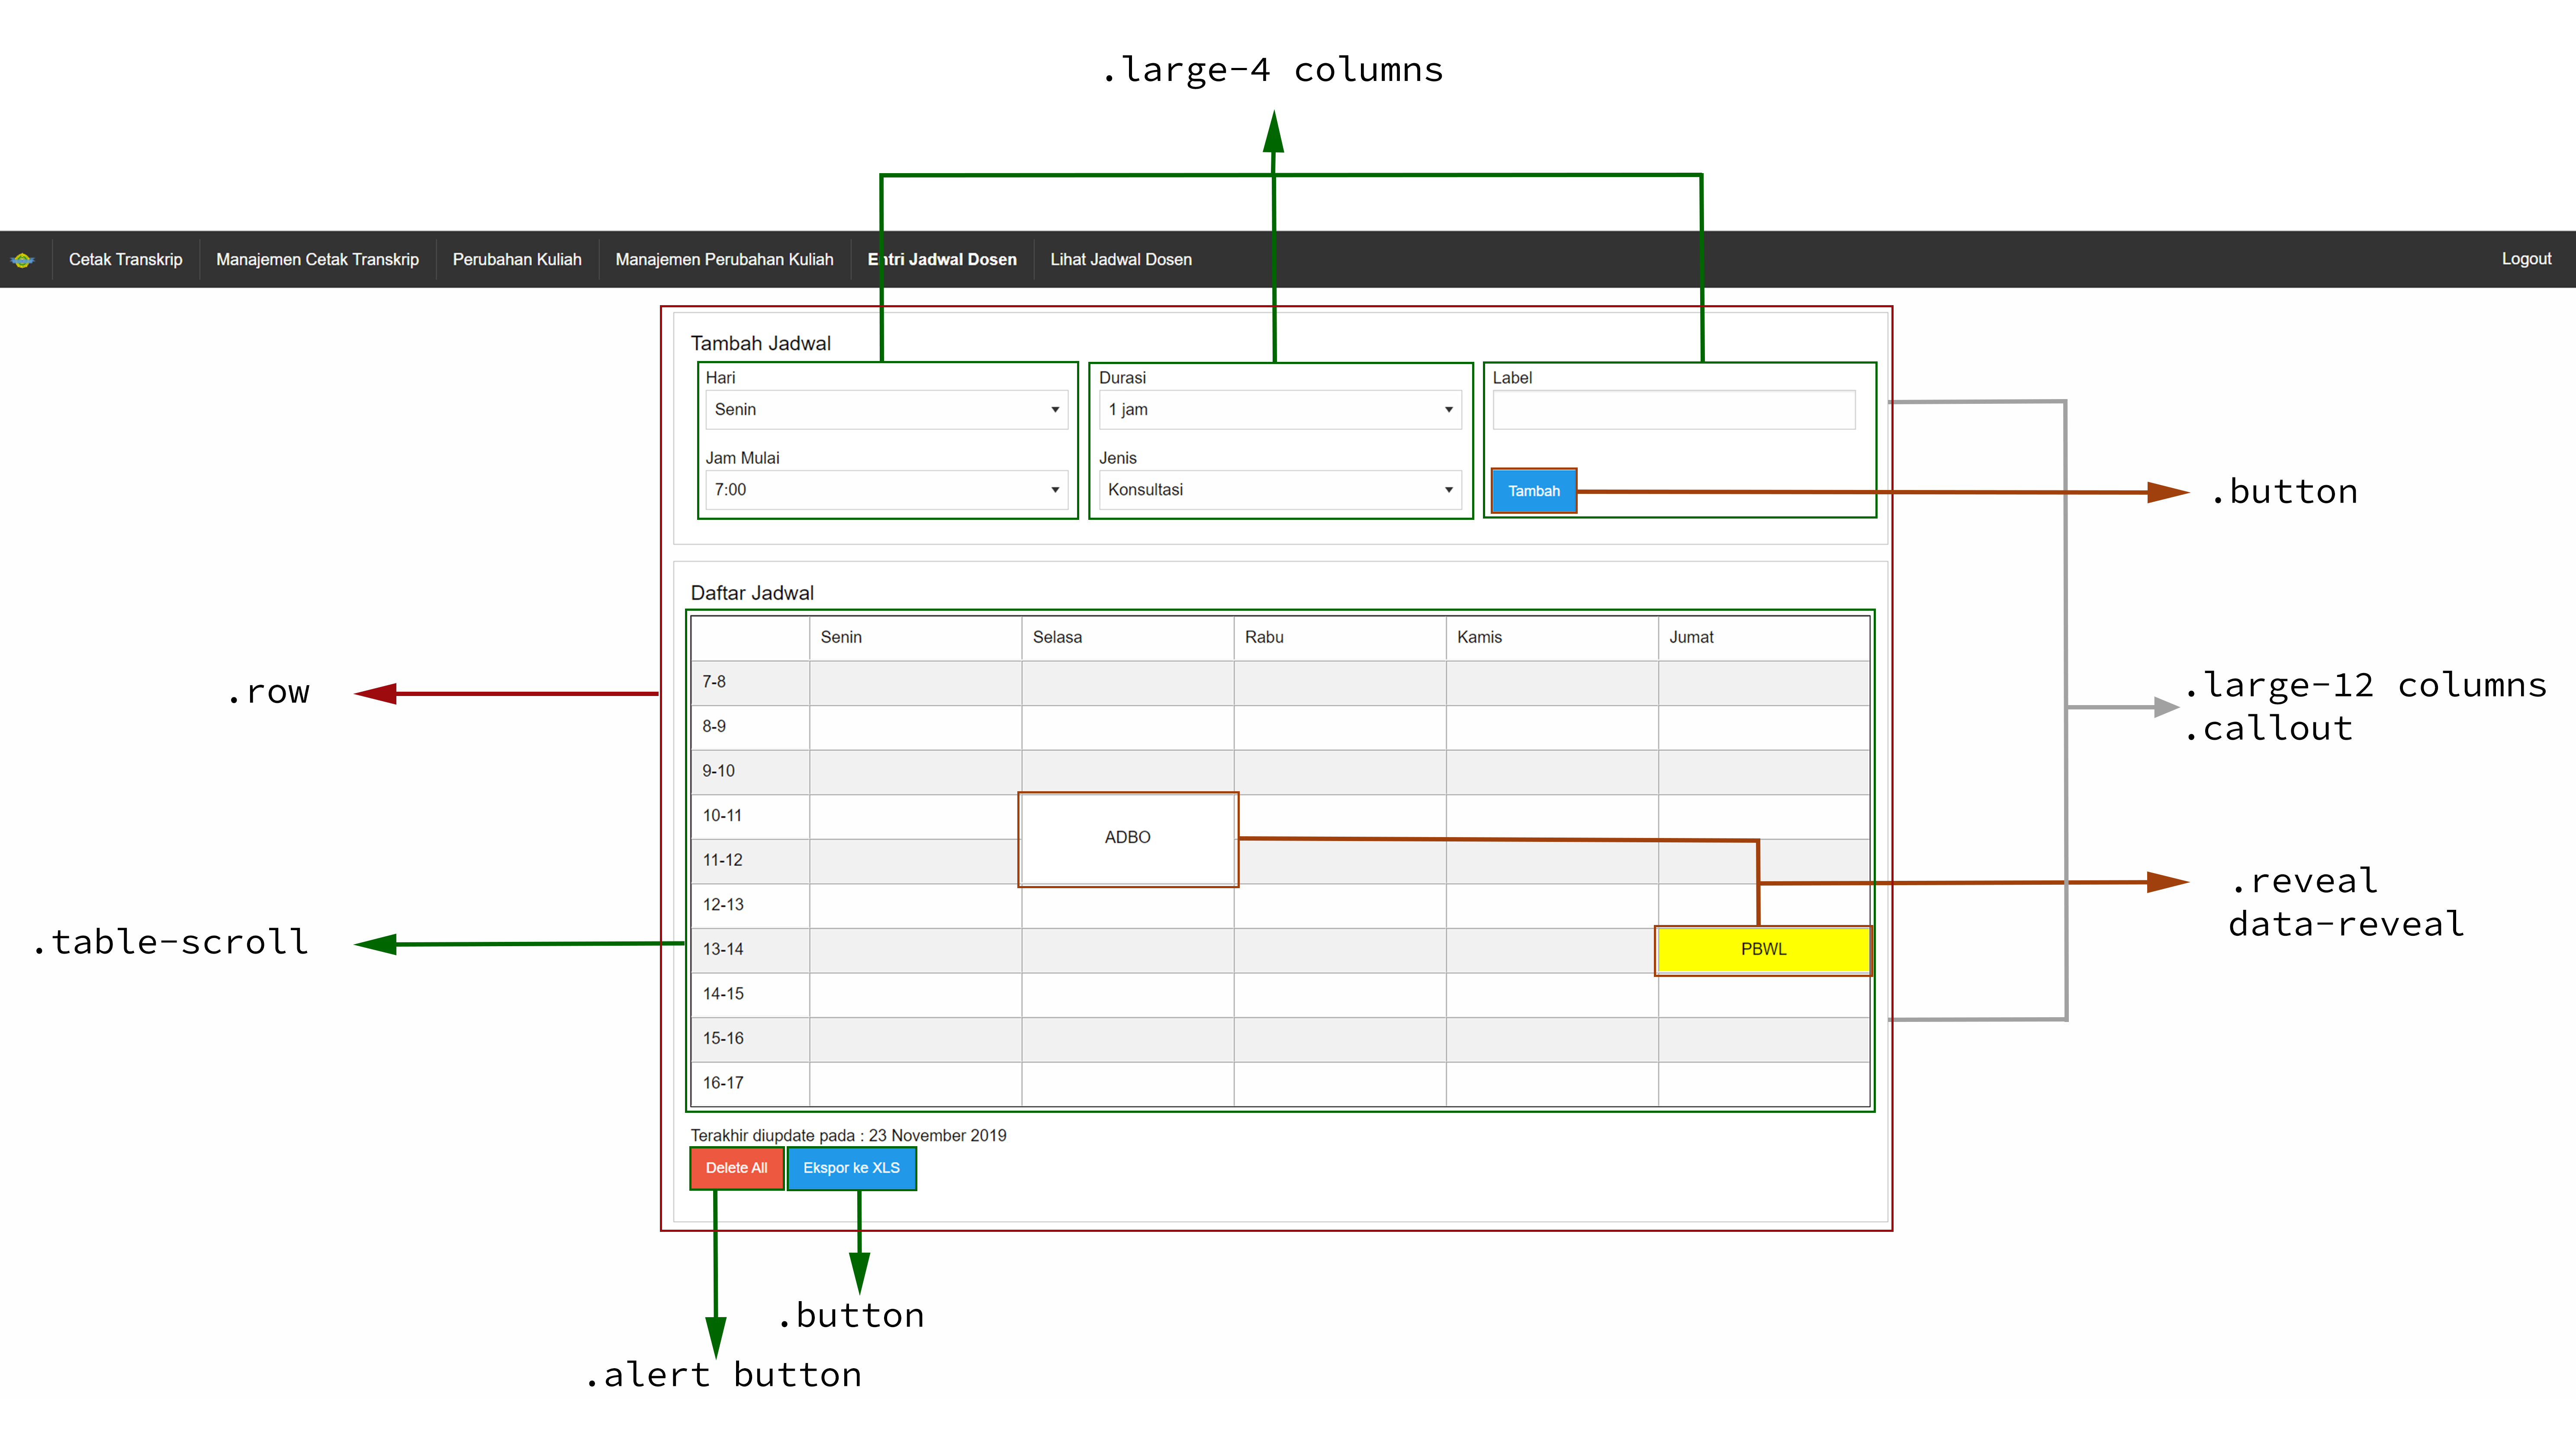
\includegraphics[width=\textwidth,height=\textheight,keepaspectratio]{foundation/analisis_tampilan_entri_jadwal_dosen.png}
	\caption{Analisis halaman entri jadwal dosen.}
	\label{fig:analisisEntriJadwalDosen}
\end{figure}
Kelas - kelas yang digunakan dalam halaman entri jadwal dosen tertera pada tabel ~\ref{table:analisisEntriJadwalDosen}:
\begin{table}[H]
	\centering
	\caption{Penggunaan kelas pada halaman entri jadwal dosen.}
	\begin{tabularx}{\textwidth}{lX}
		\toprule
		Kelas     & Penggunaan \\
		\midrule
		\texttt{.row} & Kelas ini memiliki dua fungsi sebagai container konten dan mengatur beberapa \textit{field-form} menjadi satu baris. \\
		\texttt{.large-4 column} & Setiap field akan pada \textit{form} Tambah Jadwal akan memiliki lebar masing-maisng 4 grid pada layar \textit{large}.\\
		\texttt{.large-12 column} & Konten Tambah Jadwal dan Daftar Jadwal memiliki lebar 12 grid.\\
		\texttt{.callout} & Untuk membuat border yang memisahkan konten tambah jadwal dan detail jadwal.\\
		\texttt{.table-scroll} & Membuat tabel daftar jadwal dapat digerakan secara horizontal.\\
		\texttt{button} & Membuat button pada tombol `Ekspor ke XLS' untuk konten Daftar Jadwal dan `Tambah' pada konten Tambah Jadwal.\\
		\texttt{.alert button} & Membuat button pada tombol `Delete All'.\\
		\bottomrule
	\end{tabularx}%	
	\label{table:analisisEntriJadwalDosen}
\end{table}

%Modal & edit
\subsubsection{Edit Jadwal}
Cell yang terisi dengan mata kuliah pada halaman ini dapat diedit. Gambar ~\ref{fig:analisisEditEntriJadwalDosen} merupakan modal edit yang muncul ketika sebuah jadwal dipilih. 
\begin{figure} [H]
	\centering  
	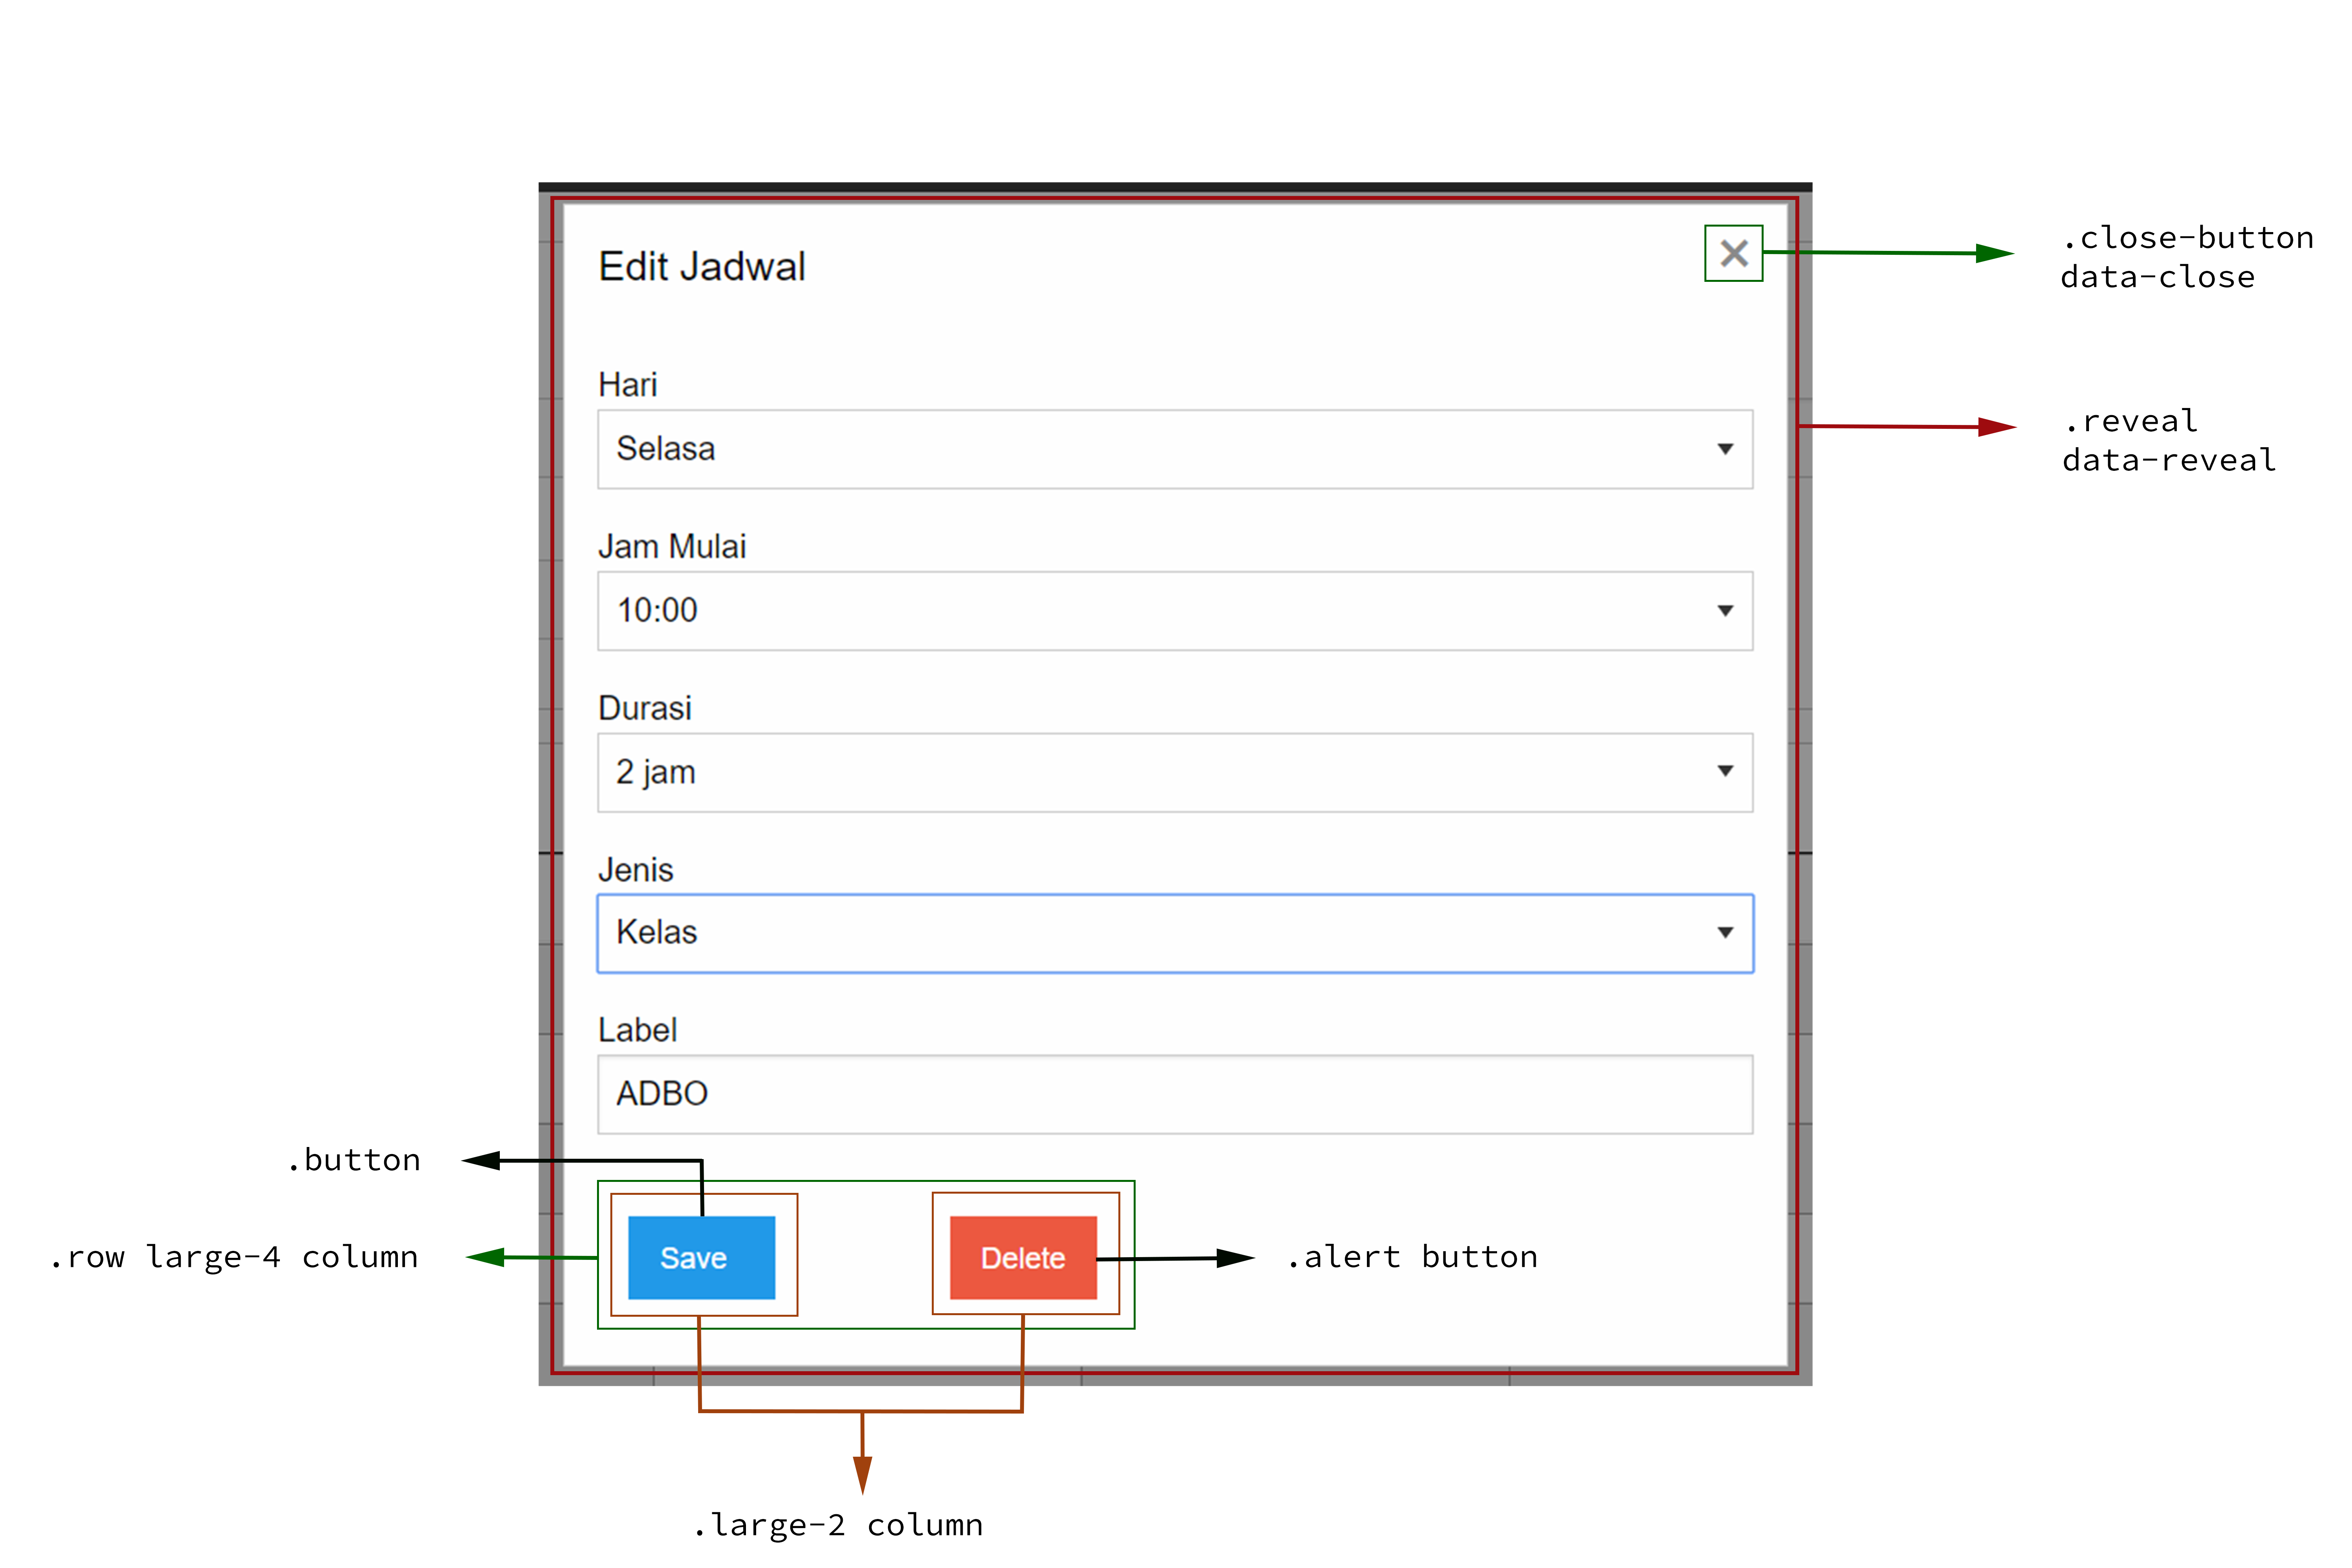
\includegraphics[width=0.6\textwidth,height=\textheight,keepaspectratio]{foundation/analisis_modal_edit_jadwal_entri_jadwal_dosen.png}
	\caption{Analisis modal edit entri jadwal dosen.}
	\label{fig:analisisEditEntriJadwalDosen}
\end{figure}

Kelas yang digunakan modal edit jadwal dosen tertera pada tabel ~\ref{table:analisisEditEntriJadwalDosen}:
\begin{table}[H]
	\centering
	\caption{Penggunaan kelas pada modal edit jadwal dosen.}
	\begin{tabularx}{\textwidth}{lX}
		\toprule
		Kelas     & Penggunaan \\
		\midrule
		\texttt{.reveal data-reveal} & Membuat modal yang menampung tabel detail permohonan.\\
		\texttt{.close-button data-close aria-label} & Menutup modal yang telah terbuka dengan memberikan label `x' pada tombol.\\
		\texttt{.large-4 column} & Kolom tombol akan memiliki lebar 4 grid pada layar \textit{large}.\\
		\texttt{.large-2 column} & Masing - masing tombol `Save' dan `Delete' akan memiliki lebar 2 grid pada layar \textit{large}.\\
		\texttt{.button} & Membuat button `Save'.\\
		\texttt{.alert button} & Membuat button `Delete'.\\
		\bottomrule
	\end{tabularx}%	
	\label{table:analisisEditEntriJadwalDosen}
\end{table}


\subsection{Halaman Lihat Jadwal Dosen}
\noindent Gambar ~\ref{fig:analisisLihatJadwalDosen} merupakan halaman lihat jadwal dosen berisi sebuah tabs, dimana setiap judul tabs yang berada diatas tabel mereferensikan ke \texttt{tabs-content} atau halaman jadwal setiap dosen. Kemudian pada bagian bawah tabel terdapat tombol biru "Ekspor ke XLS".
\subsubsection{Halaman Utama}
\begin{figure} [H]
	\centering  
	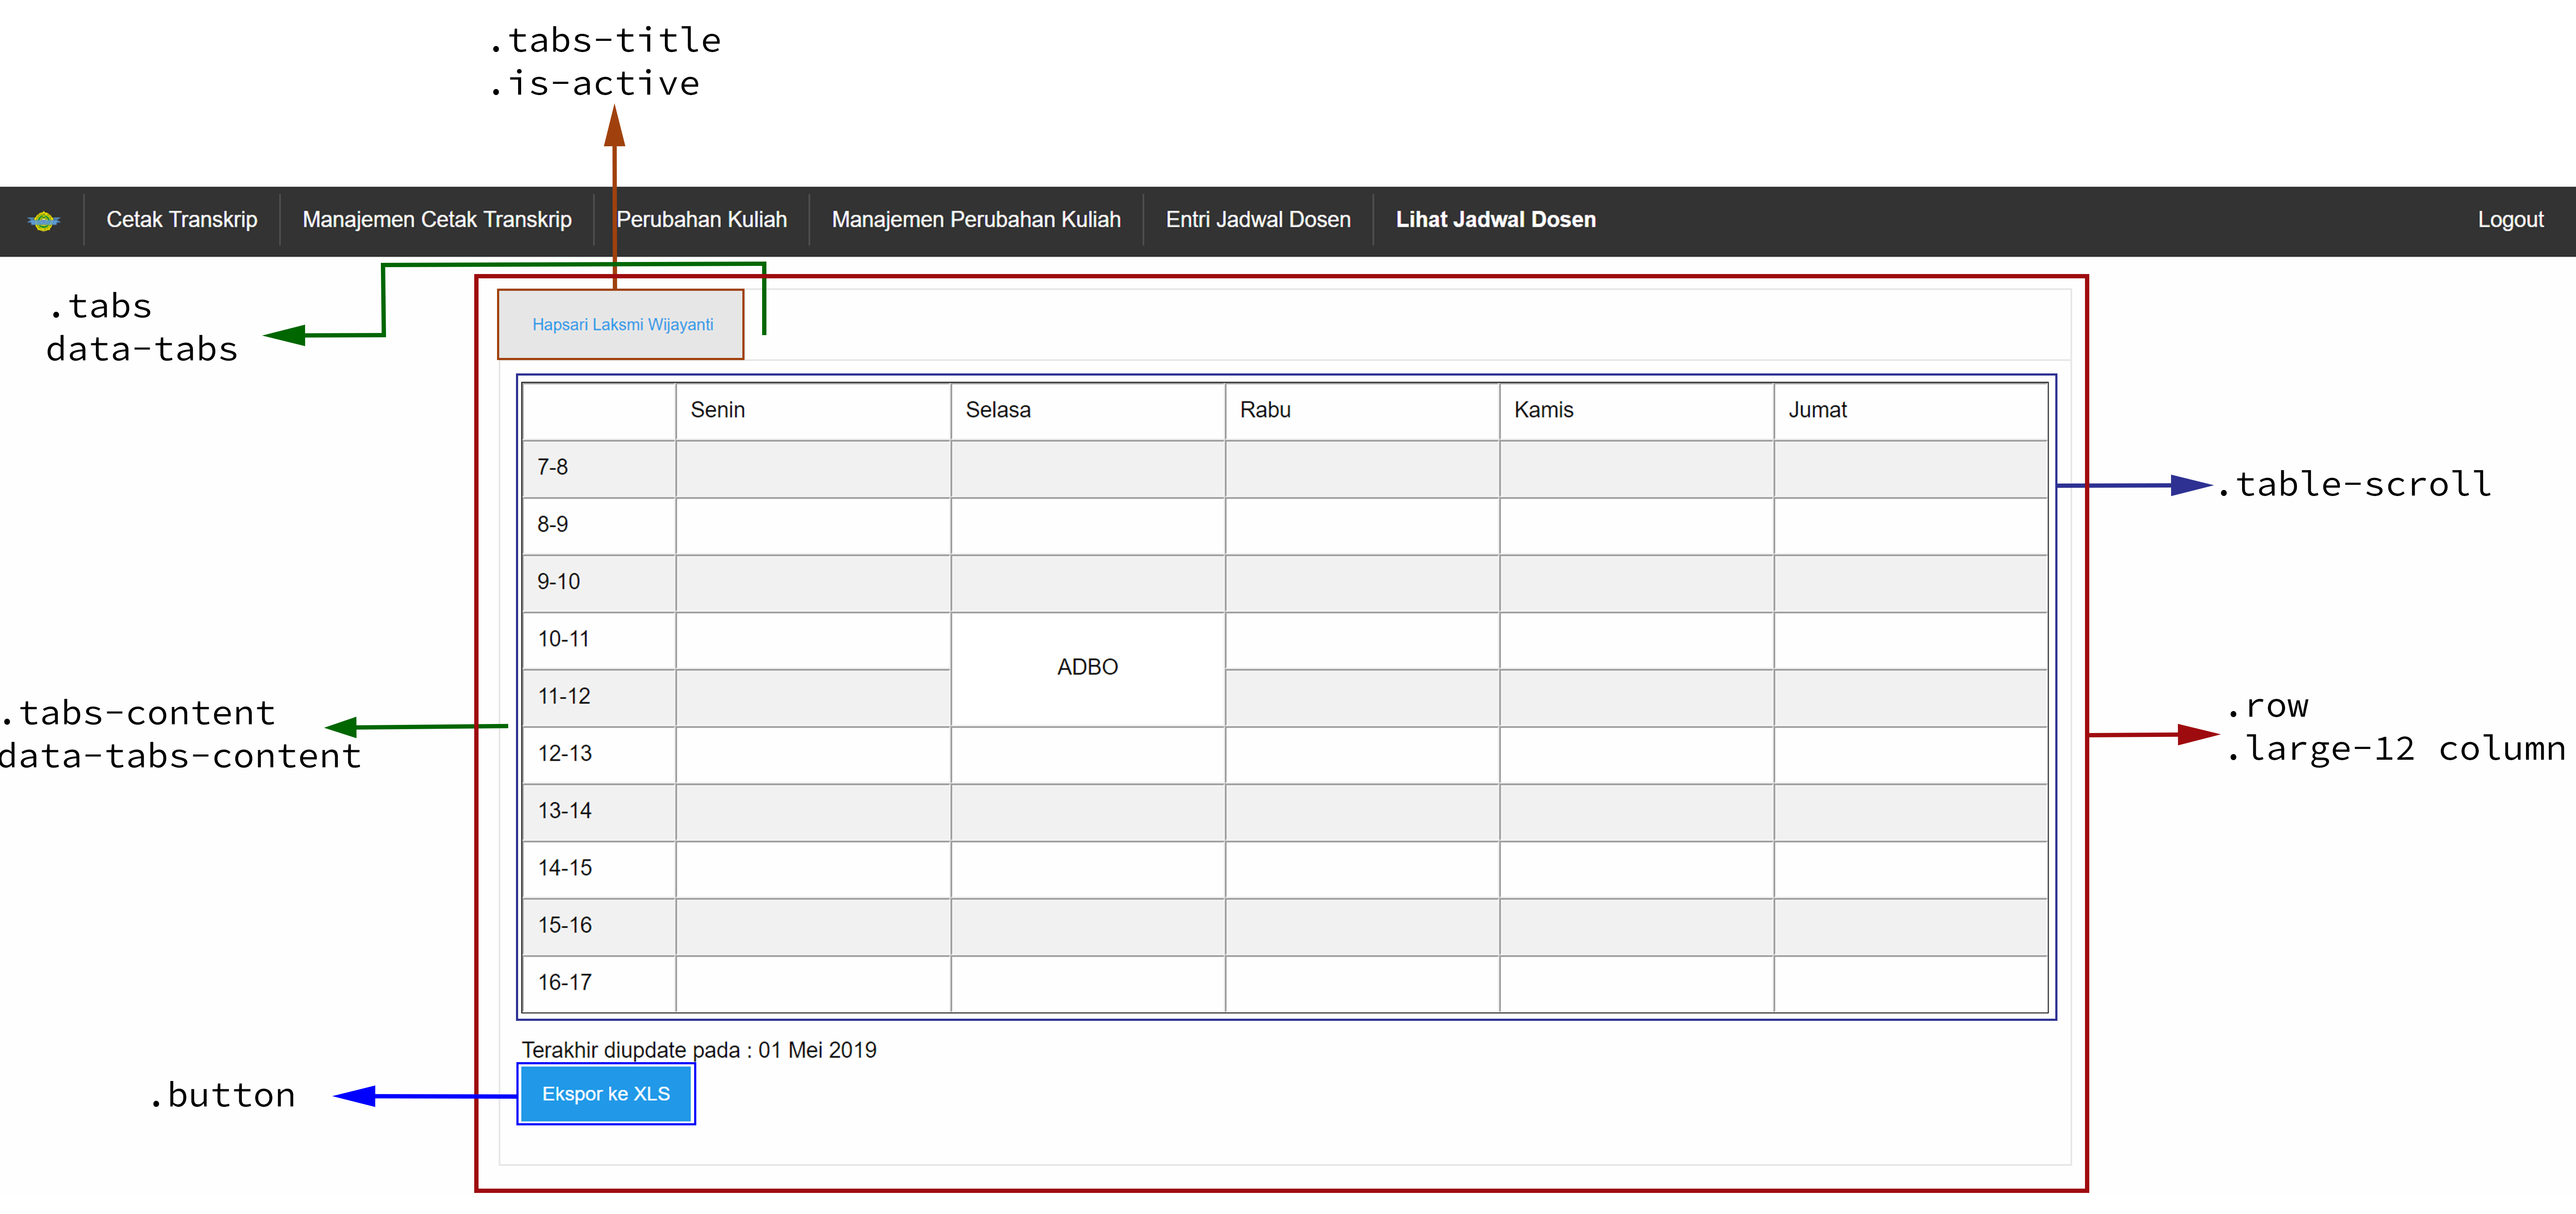
\includegraphics[width=\textwidth,height=\textheight,keepaspectratio]{foundation/analisis_tampilan_lihat_jadwal_dosen.png}
	\caption{Analisis halaman lihat jadwal dosen.}
	\label{fig:analisisLihatJadwalDosen}
\end{figure}

\noindent Kelas-kelas yang digunakan pada modal edit jadwal dosen tertera pada tabel ~\ref{table:analisisLihatJadwalDosen}:
\begin{table}[H]
	\centering
	\caption{Penggunaan kelas pada halaman lihat jadwal dosen.}
	\begin{tabularx}{\textwidth}{lX}
		\toprule
		Kelas     & Penggunaan \\
		\midrule
		\texttt{.row} & Kelas ini memiliki dua fungsi sebagai container konten dan mengatur beberapa \textit{field-form} menjadi satu baris. \\
		\texttt{.large-12 column} & Konten Tambah Jadwal dan Daftar Jadwal memiliki lebar 12 grid.\\
		\texttt{.callout} & Untuk membuat border yang memisahkan konten tambah jadwal dan detail jadwal.\\
		\texttt{.table-scroll} & Membuat tabel lihat jadwal dapat digerakan secara horizontal.\\
		\texttt{button} & Membuat button pada tombol `Ekspor ke XLS' untuk konten Daftar Jadwal dan `Tambah' pada konten Tambah Jadwal.	\\
		\texttt{.tabs data-tabs} & Kontainer untuk simpan nama dosen\\
		\texttt{.tabs-content data-tabs-content} & Kontainer untuk simpan isi konten dari tabs.\\
		\texttt{.tabs-title} & Kelas untuk tabs nama-nama dosen.\\
		\texttt{.is-active} & Menujukkan tabs nama dosen yang sedang dilihat.\\
		\bottomrule
	\end{tabularx}%	
	\label{table:analisisLihatJadwalDosen}
\end{table}

\section{Perancangan Halaman Website dengan Bootstrap 4}
Setelah menganalisis kelas apa saja yang digunakan dalam website, pada bagian ini akan ditampilkan rancangan penggunaan kelas - kelas dengan menggunakan Bootstrap 4. Perancangan akan dibuat dalam bentuk visual yaitu screenshot setiap halaman dan kelas yang nantinya digunakan dalam tahap implementasi. Selain itu dipaparkan tabel perbandingan antara kelas yang dahulu digunakan dan kelas yang akan digunakan pada tahap implementasi.\\
\subsection{Halaman Login}
\noindent Gambar ~\ref{fig:konversiLogin} menjelaskan komponen dalam website beserta penamaan kelas untuk Bootstrap 4 pada halaman login.\\
\begin{figure} [H]
	\centering  
	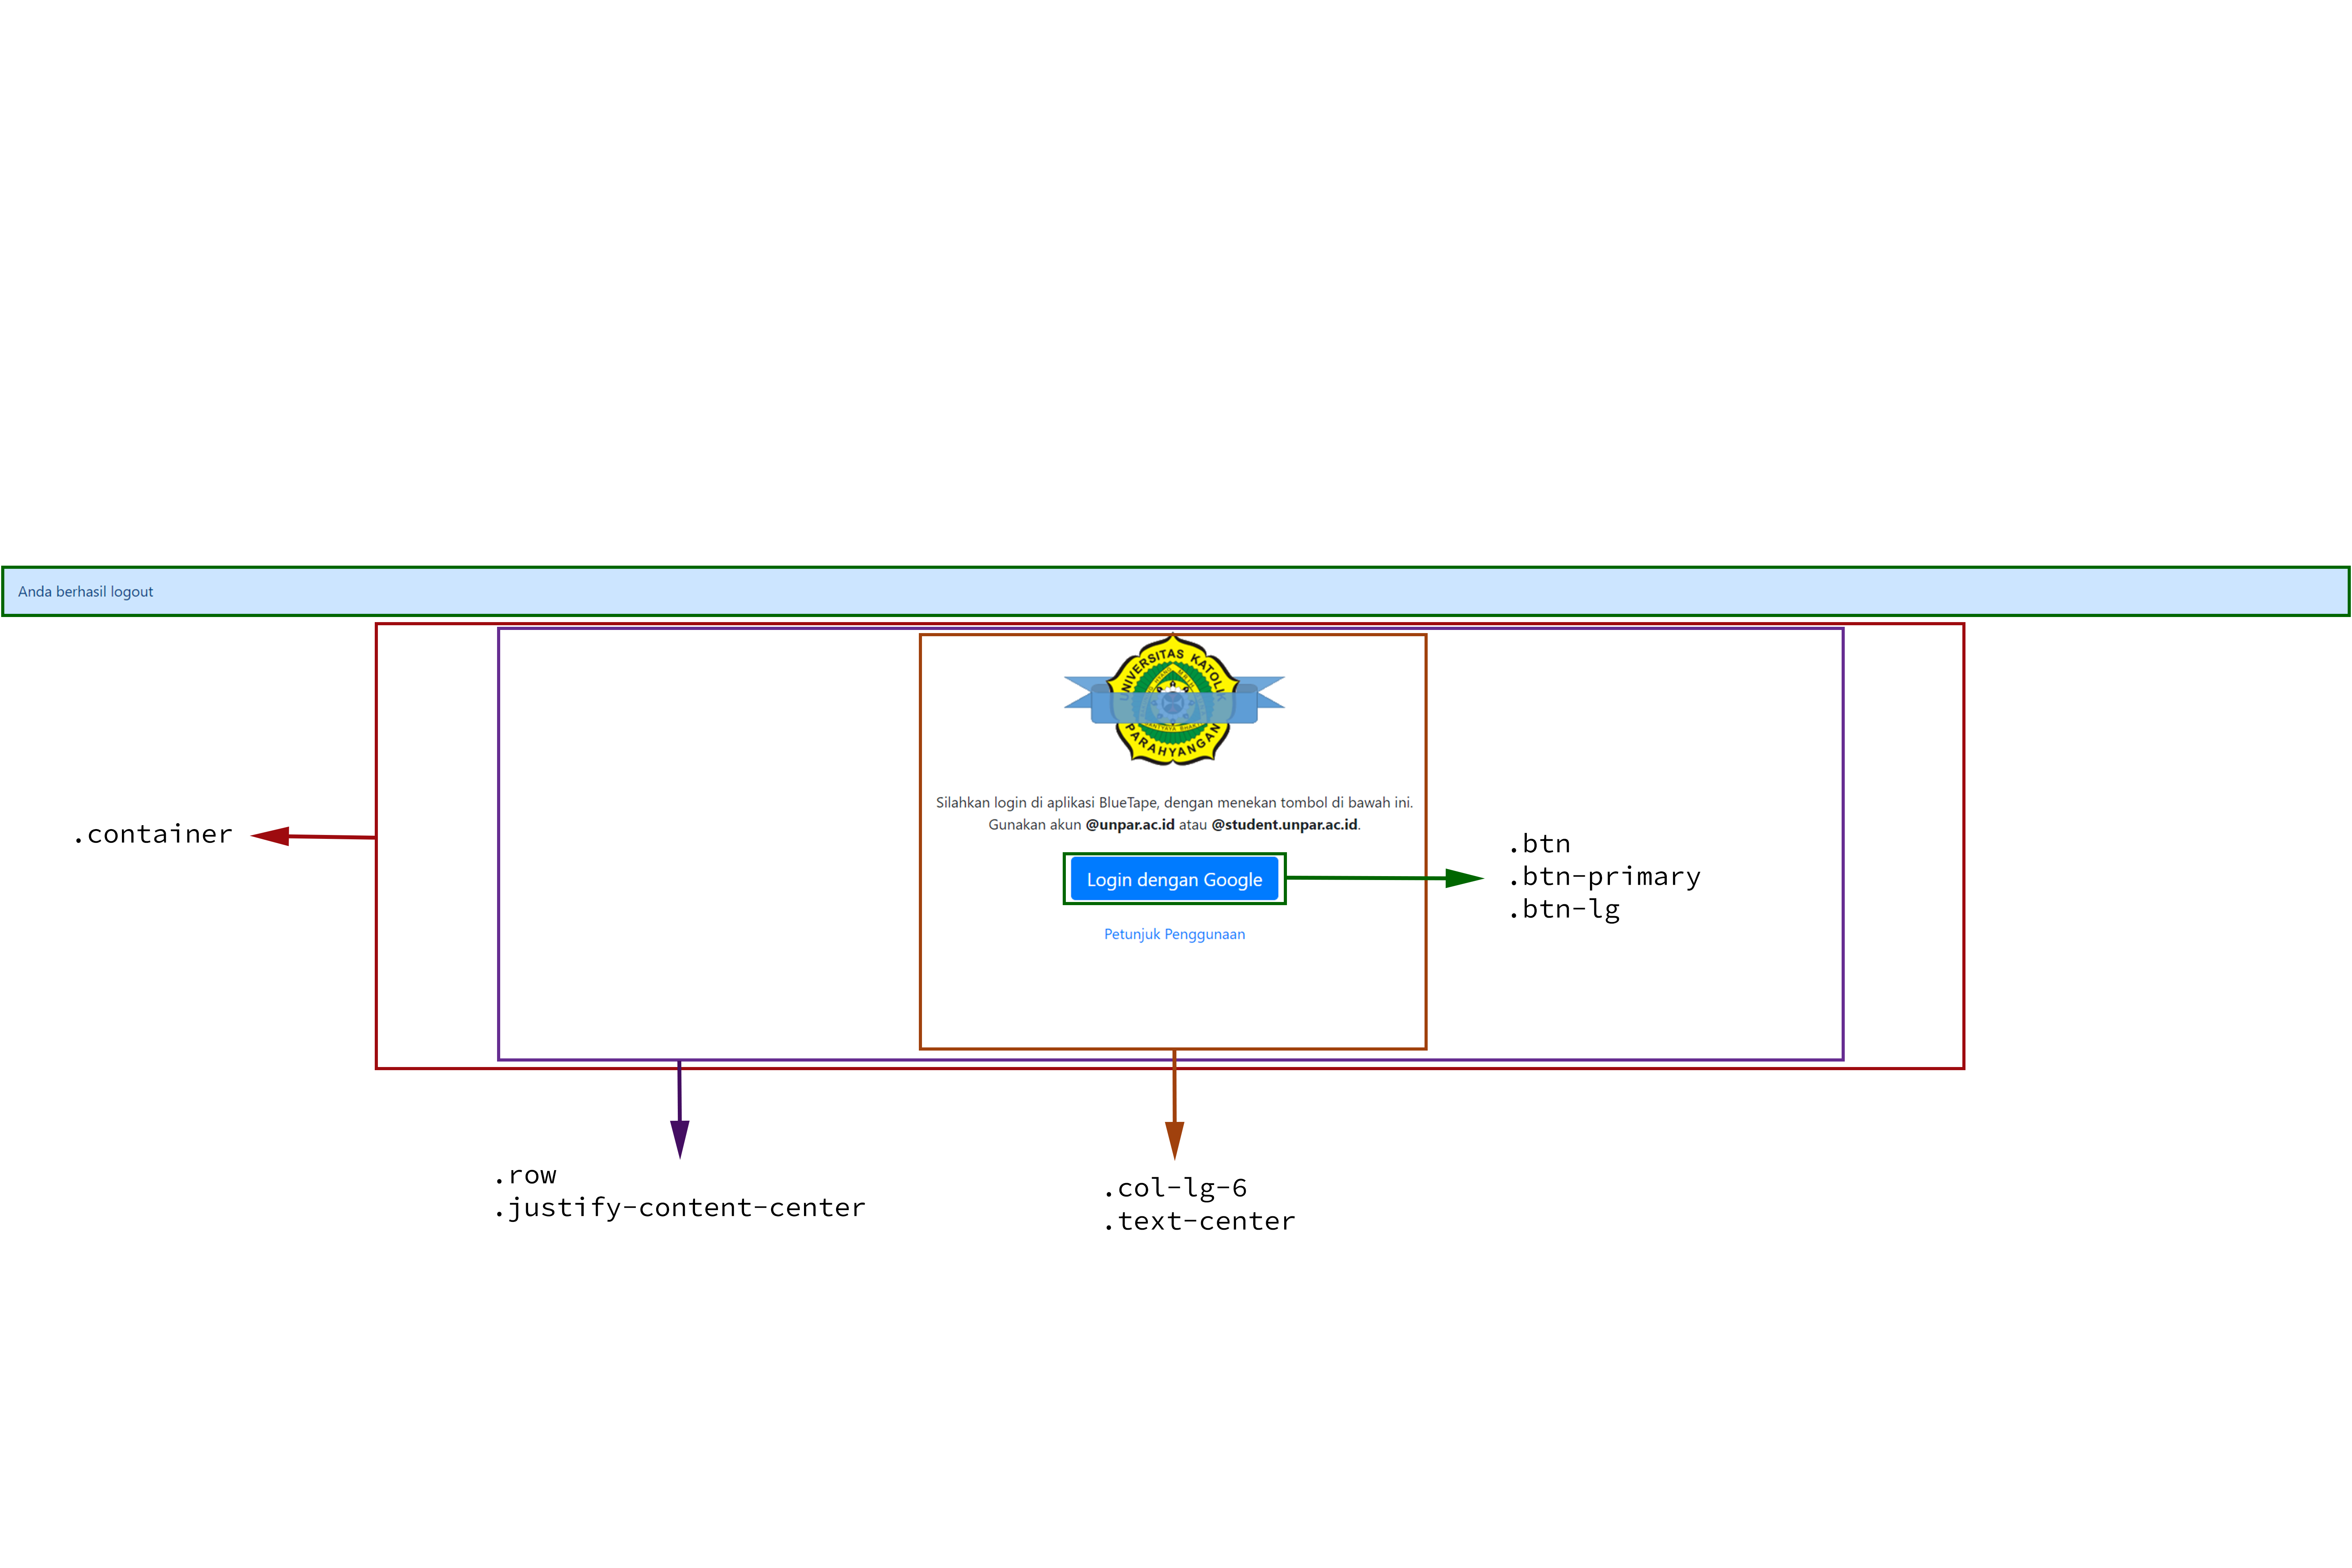
\includegraphics[width=\textwidth,height=\textheight,keepaspectratio]{bootstrap/konversi_tampilan_login.png}  
	\caption{Konversi halaman login.} 
	\label{fig:konversiLogin}
\end{figure} \noindent \\

\noindent Perbandingan penggunaan kelas pada Foundation 6 dan Bootstrap 4 pada halaman login tertera pada tabel ~\ref{table:konversiLogin}.\\
\begin{table}[H]
	\caption{Tabel konversi pada halaman login.}
	\begin{tabular}{| p{0.35\textwidth} | p{0.27\textwidth} | p{0.27\textwidth} |} 
		\hline
		\textbf{Jenis Komponen} & \textbf{Foundation 6} & \textbf{Bootstrap 4}  \\ [0.5ex] 
		\hline
		Grid untuk menampung konten & \texttt{.row}, \texttt{.column} &\texttt{.container}    \\	
		& \texttt{.row} &\texttt{.row}     \\  
		\hline
		Konten berada di tengah &\texttt{.large-centered} &\texttt{.justify-content-center} \\  
		\hline
		Grid dengan lebar 6 &\texttt{.large-6} &\texttt{.col-lg-6}    \\ 
		\hline
		Posisi text rata tengah  &\texttt{.text-center} & \texttt{.text-center }  \\ 
		\hline
		Tombol berwarna biru &\texttt{.button} & \texttt{.btn}   \\ 
		\hline
		Tombol selebar konten & \texttt{.btn expand} & \texttt{.btn-lg}  \\ 
		\hline
		Label berwarna merah & \texttt{.callout alert} & \texttt{.alert alert-primary}  \\ 
		\hline
		Label berwarna biru & \texttt{.callout primary} & \texttt{.alert alert-danger}  \\ [1ex]
		\hline
	\end{tabular}
	\label{table:konversiLogin}
\end{table}


\subsection{Menu Navigasi}
\noindent Gambar ~\ref{fig:konversiNavigasi} menjelaskan komponen dalam website beserta penamaan kelas untuk Bootstrap 4 pada menu navigasi.\\
\begin{figure} [H]
	\centering  
	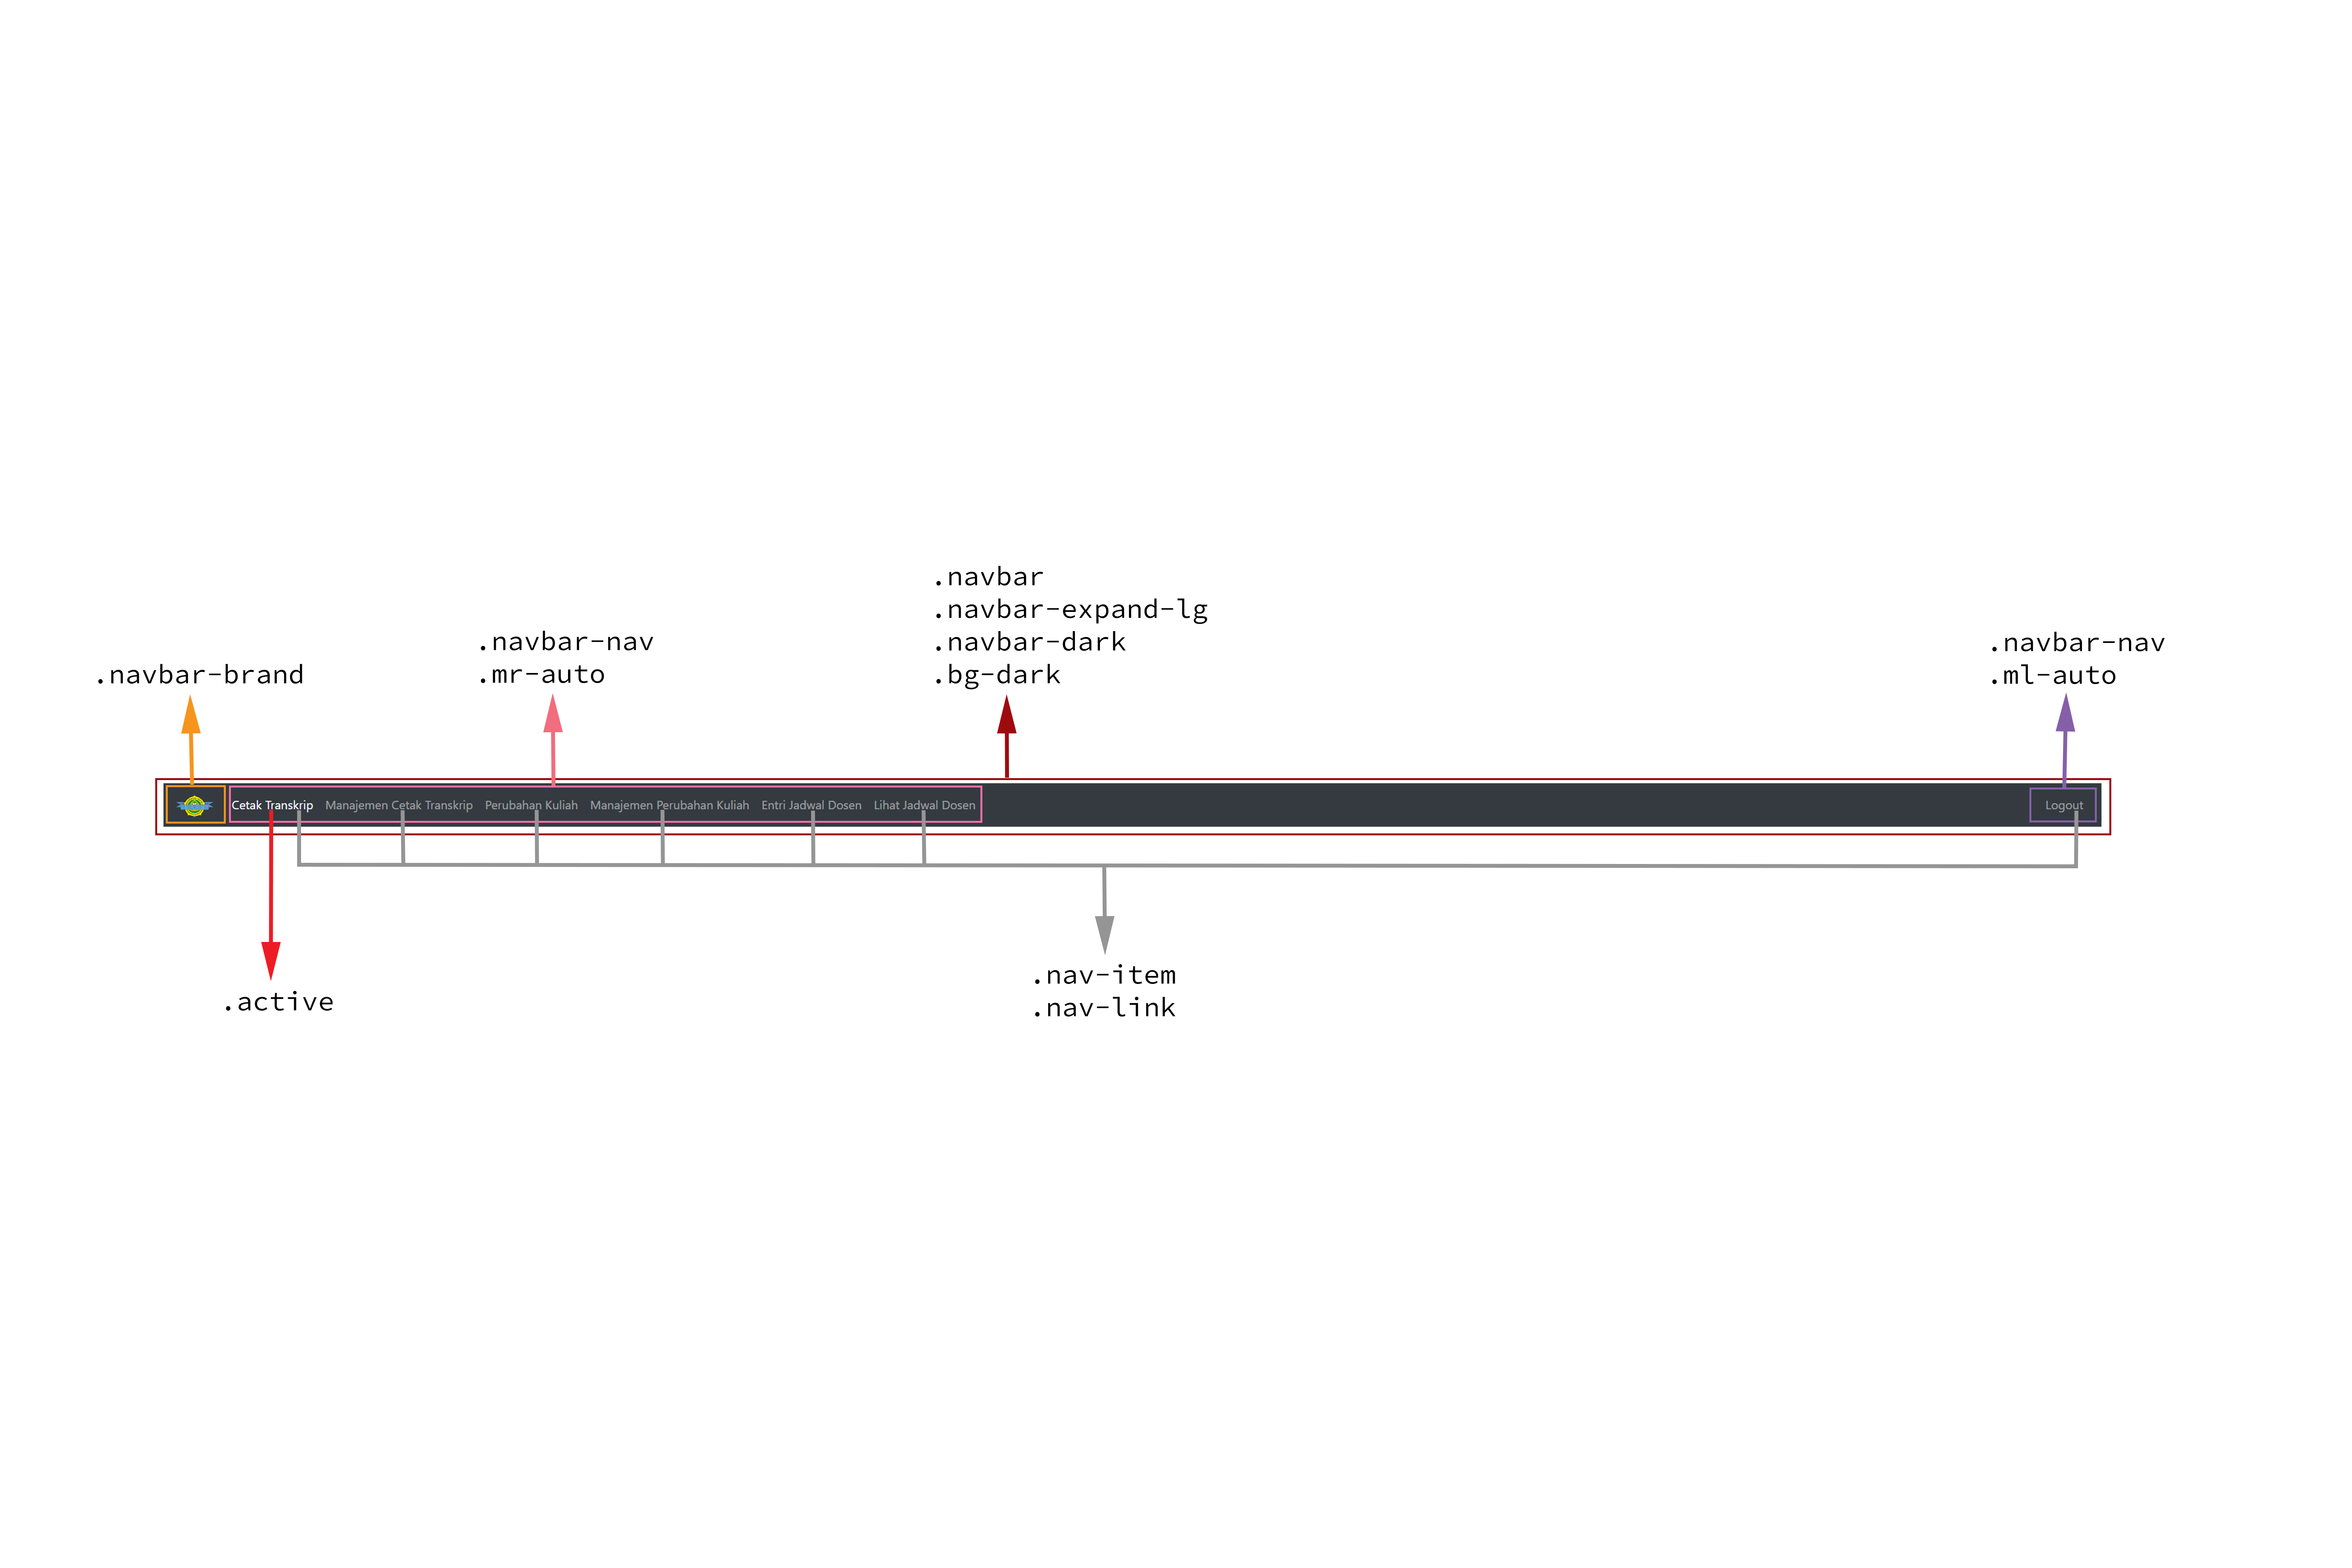
\includegraphics[width=\textwidth,height=\textheight,keepaspectratio]{bootstrap/konversi_navbar.png}  
	\caption{Konversi menu navigasi di layar \textit{large}.} 
	\label{fig:konversiNavigasi}
\end{figure}

\noindent Perbandingan penggunaan kelas pada Foundation 6 dan Bootstrap 4 pada menu navigasi tertera pada tabel ~\ref{table:konversiNavigasi}.\\
\begin{table}[H]
	\caption{Tabel konversi pada menu navigasi di layar \textit{large}.}
	\begin{tabular}{| p{0.35\textwidth} | p{0.27\textwidth} | p{0.27\textwidth} |} 
		\hline
		\textbf{Jenis Komponen} & \textbf{Foundation 6} & \textbf{Bootstrap 4}  \\ [0.5ex] 
		\hline	
		 Judul website & \texttt{.title-bar-title }& \texttt{.navbar-brand}  \\ 
		\hline
		Menu &\texttt{.menu }& \texttt{.top-bar } \\
		\hline
		Sub-menu terpilih & \texttt{.menu-active} & \texttt{.active}  \\
		\hline	
		Kelas untuk setiap menu & \texttt{.menu-text} & \texttt{.nav-item .nav-link} \\
		\hline	
		Menu berada di kiri & \texttt{.top-bar-left} & \texttt{.ml-auto}  \\
		\hline
		Menu berada di kanan & \texttt{.top-bar-right} & \texttt{.mr-auto}  \\
		\hline
		Tema untuk menu & - & \texttt{.navbar-dark .bg-dark}\\ [1ex] 
		\hline
	\end{tabular}
	\label{table:konversiNavigasi}
\end{table}

\begin{figure} [H]
	\centering  
	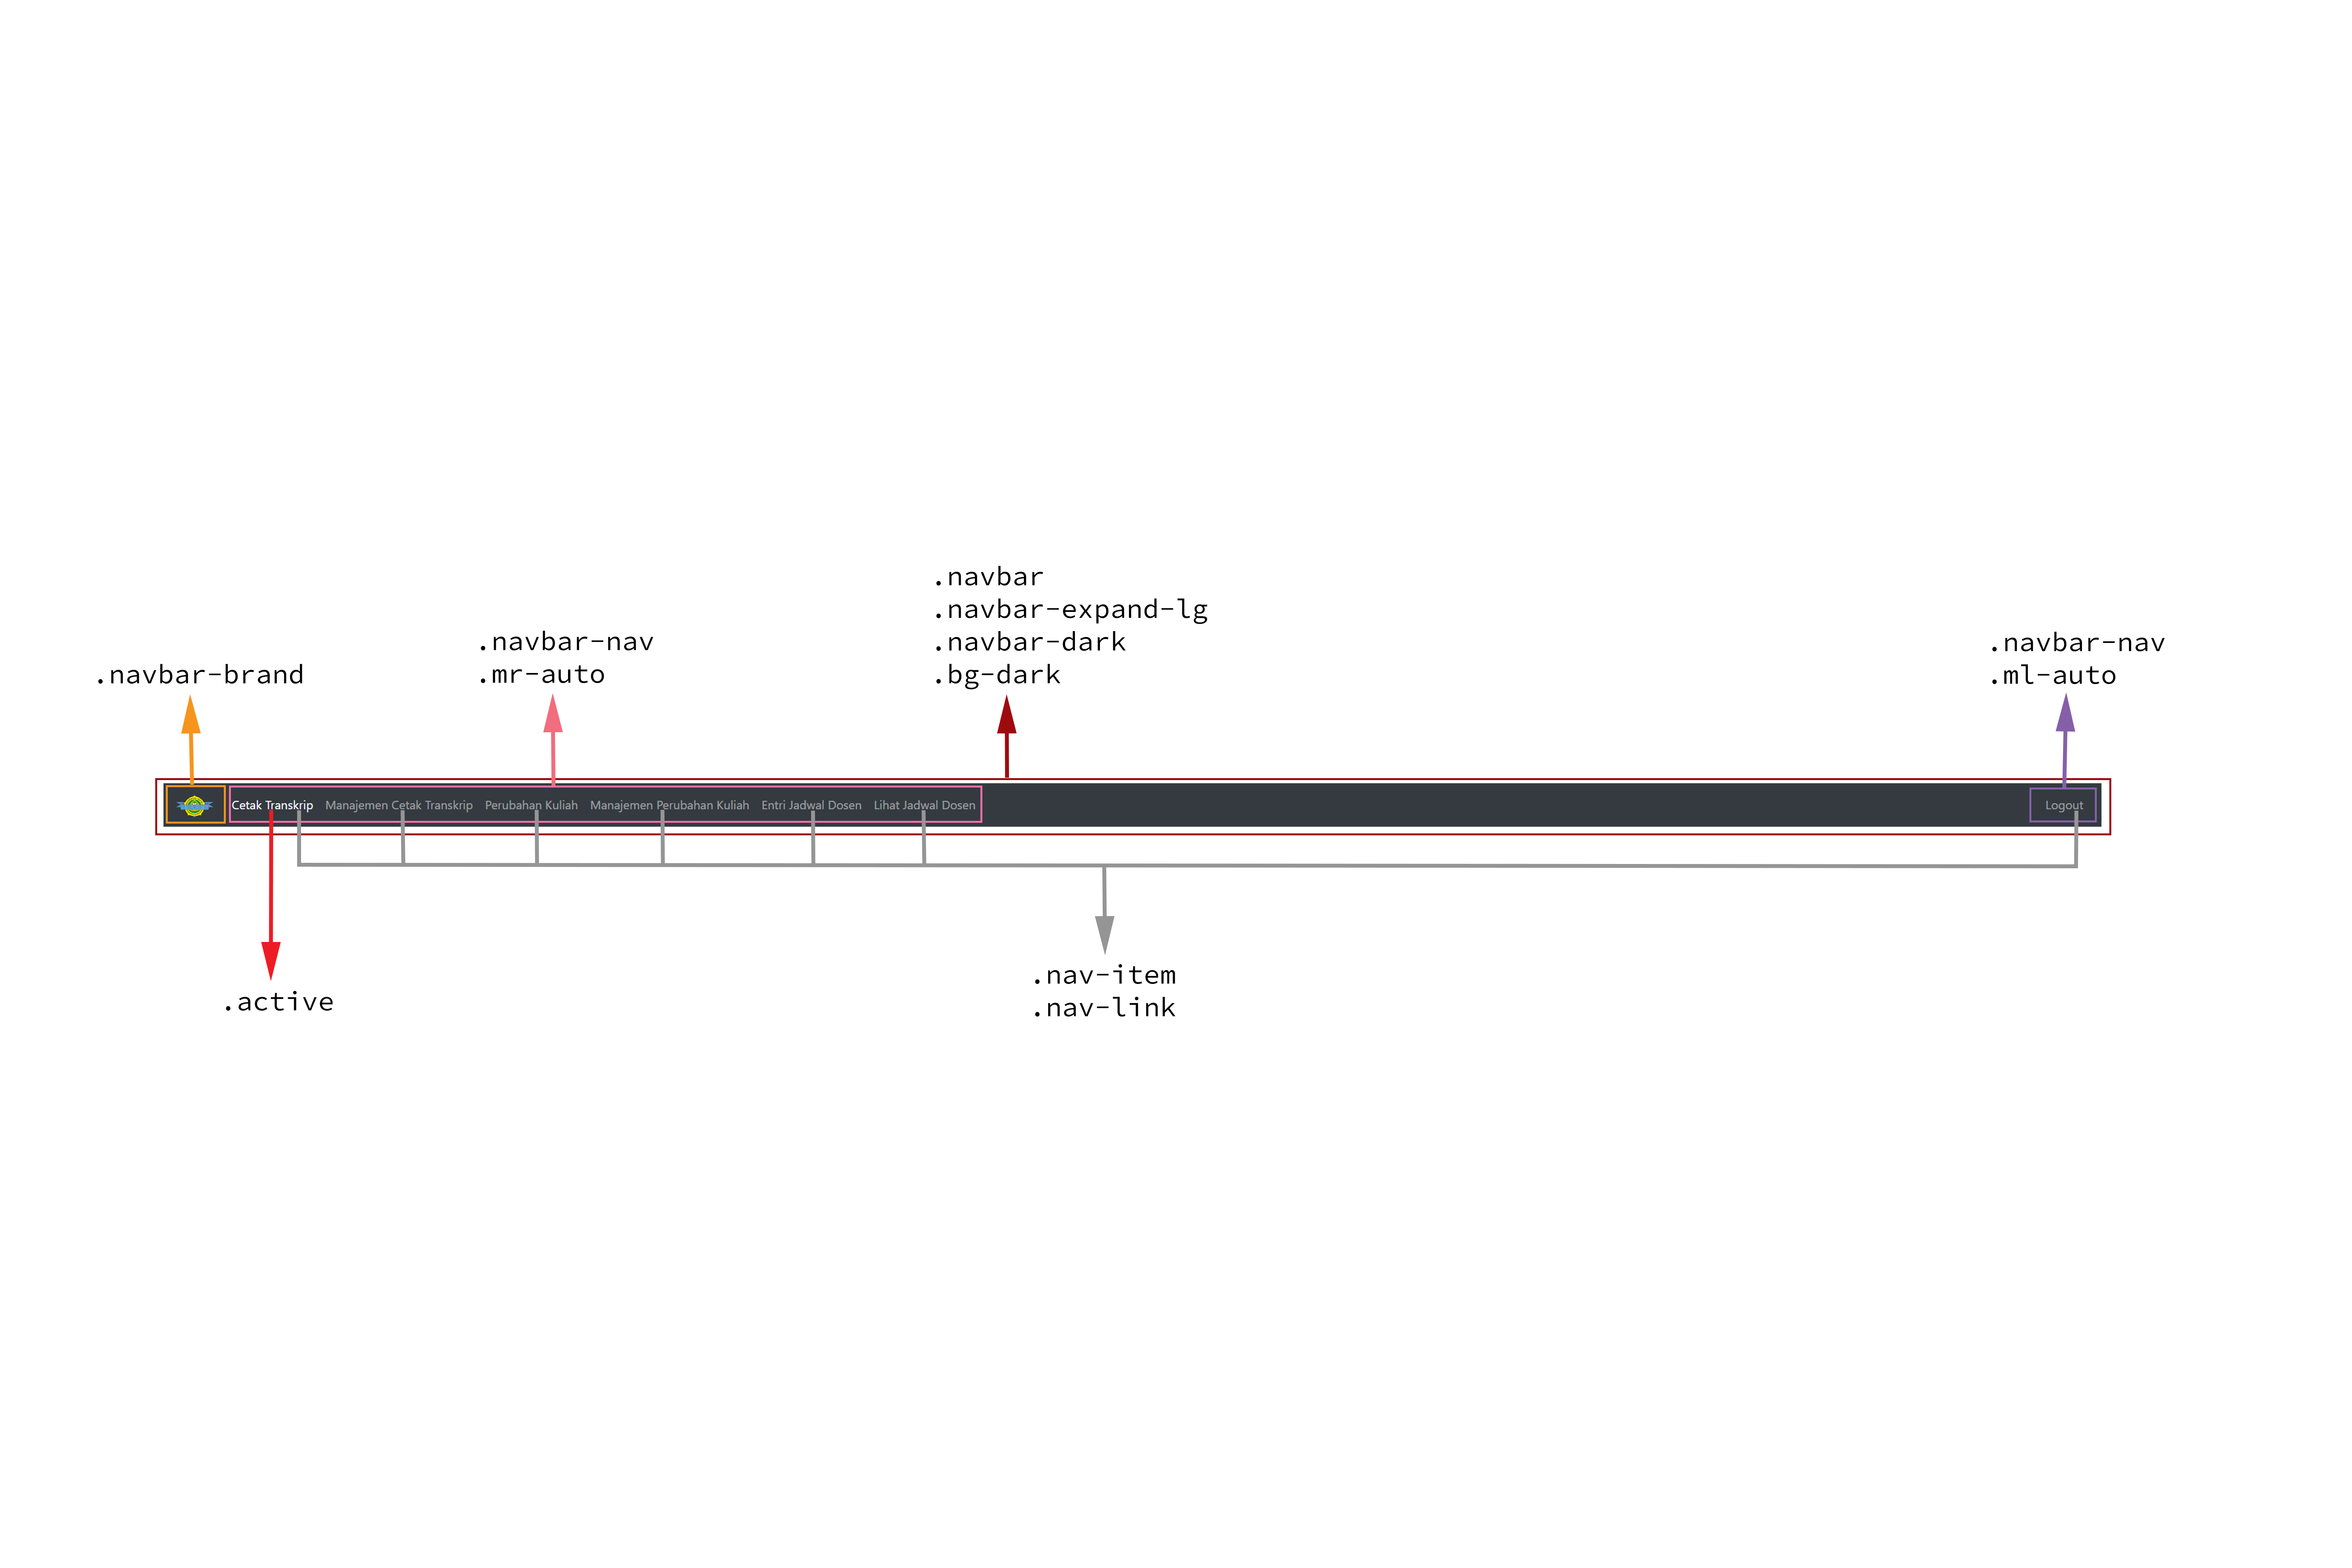
\includegraphics[width=\textwidth,height=\textheight,keepaspectratio]{bootstrap/konversi_navbar.png}  
	\caption{Konversi menu navigasi di layar \textit{small} dan \textit{medium}.} 
	\label{fig:konversiNavigasiSmall}
\end{figure}

\noindent Perbandingan penggunaan kelas pada Foundation 6 dan Bootstrap 4 pada menu navigasi tertera pada tabel ~\ref{table:konversiNavigasiSmall}.\\
\begin{table}[H]
	\caption{Tabel konversi pada menu navigasi di layar \textit{medium} dan \textit{small}.}
	\begin{tabular}{| p{0.35\textwidth} | p{0.27\textwidth} | p{0.27\textwidth} |} 
		\hline
		\textbf{Jenis Komponen} & \textbf{Foundation 6} & \textbf{Bootstrap 4}  \\ [0.5ex] 
		\hline	
		Aksi \textit{collapse} menu & \texttt{.title-bar} \texttt{data-responsive-toggle} \texttt{data-hide-for} & \texttt{.collapse} \texttt{.navbar-collapse}  \\ 
		\hline
		Menu dropdown & \texttt{.menu }& \texttt{.navbar-toggler } \\
		\hline
		Ikon menu & \texttt{.menu-icon} \texttt{data-toggle} & \texttt{.navbar-toggler-icon}  \\ [1ex] 
		\hline
	\end{tabular}
	\label{table:konversiNavigasiSmall}
\end{table}

\subsection{Halaman Permintaan Cetak Transkrip}
\noindent Gambar ~\ref{fig:konversiPermintaanCetakTranskrip} menjelaskan komponen dalam website beserta penamaan kelas untuk Bootstrap 4 pada halaman permintaan cetak transkrip.\\

\subsubsection{Halaman Utama}
\begin{figure} [H]
	\centering  
	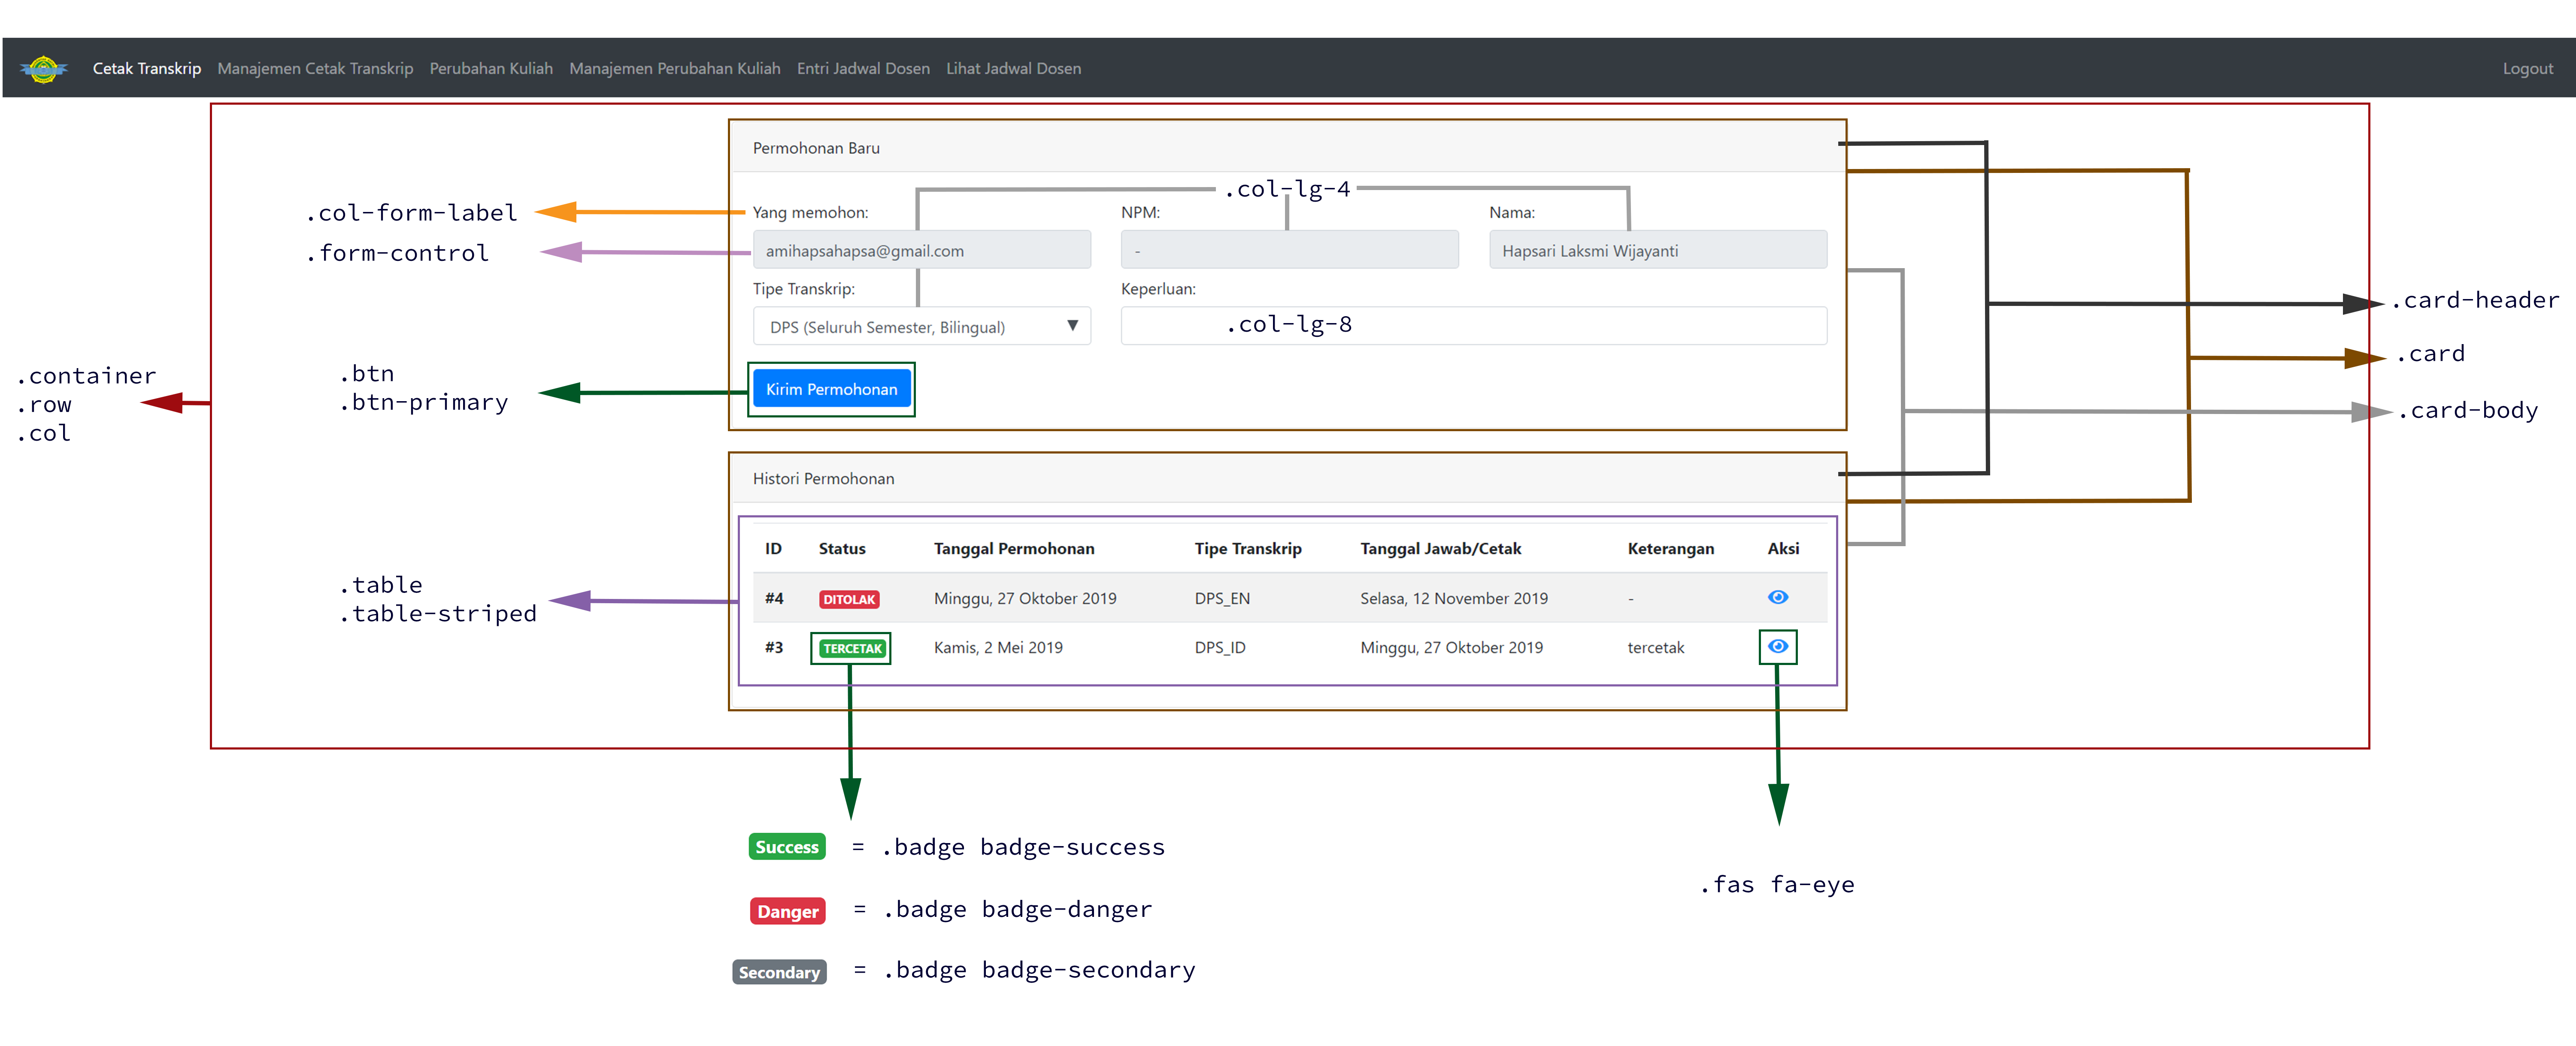
\includegraphics[width=\textwidth,height=\textheight,keepaspectratio]{bootstrap/konversi_tampilan_cetak_transkrip.png}
	\caption{Konversi halaman cetak transkrip.} 
	\label{fig:konversiPermintaanCetakTranskrip}
\end{figure}

\noindent Perbandingan penggunaan kelas pada Foundation 6 dan Bootstrap 4 pada halaman permintaan cetak transkrip tertera pada tabel ~\ref{table:konversiPermintaanCetakTranskrip}.\\ 
\begin{table}[H]
	\caption{Tabel konversi pada halaman permintaan cetak transkrip.}
	\begin{tabular}{| p{0.35\textwidth} | p{0.27\textwidth} | p{0.27\textwidth} |} 
		\hline
		\textbf{Jenis Komponen} & \textbf{Foundation 6} & \textbf{Bootstrap 4}  \\ [0.5ex] 
		\hline	
		Sistem Grid & \texttt{.row} &   \texttt{.container} \\ 
		\hline	
		Border untuk konten & \texttt{.callout} &  \texttt{.card }   \\
		&&\texttt{.card-header} \\
		&&\texttt{.card-body} \\
		\hline	
		Lebar grid pada layar \texttt{medium} & \texttt{.medium-*} &  \texttt{.col-md-*}\\
		\hline	
		Lebar grid pada layar \texttt{large} & \texttt{.larger-*} &  \texttt{.col-lg-*} \\
		\hline
		Kolom & \texttt{.column} &  \texttt{.col} \\	
		\hline	
		Tombol berwarna biru & \texttt{.button} &  \texttt{.btn btn-primary}\\
		\hline	
		Label berwarna hijau & \texttt{.label success} &  \texttt{.badge badge-success} \\
		\hline	
		Label berwarna merah & \texttt{.label alert} & \texttt{.badge badge-danger}  \\
		\hline	
		Label berwarna abu & \texttt{.label secondary } & \texttt{.badge badge-secondary } \\
		\hline	
		Ikon bentuk mata & \texttt{.fi-eye} &  \texttt{.fas fa-eye} \\	
		\hline	
		Tabel & \texttt{.stack} & \texttt{.table table-striped}  \\
		\hline	
		Nama \textit{form} & - & \texttt{.col-form-label}  \\ 
		\hline	
		Input \textit{form} & - & \texttt{.form-control}  \\ [1ex] 
		\hline
	\end{tabular}
	\label{table:konversiPermintaanCetakTranskrip}
\end{table}

\subsubsection{Modal : Lihat}
\noindent Gambar ~\ref{fig:konversiLihatPermintaanCetakTranskrip} menjelaskan komponen dalam website beserta penamaan kelas untuk Bootstrap 4 pada modal lihat halaman permintaan transkrip.\\
\begin{figure} [H]
	\centering  
	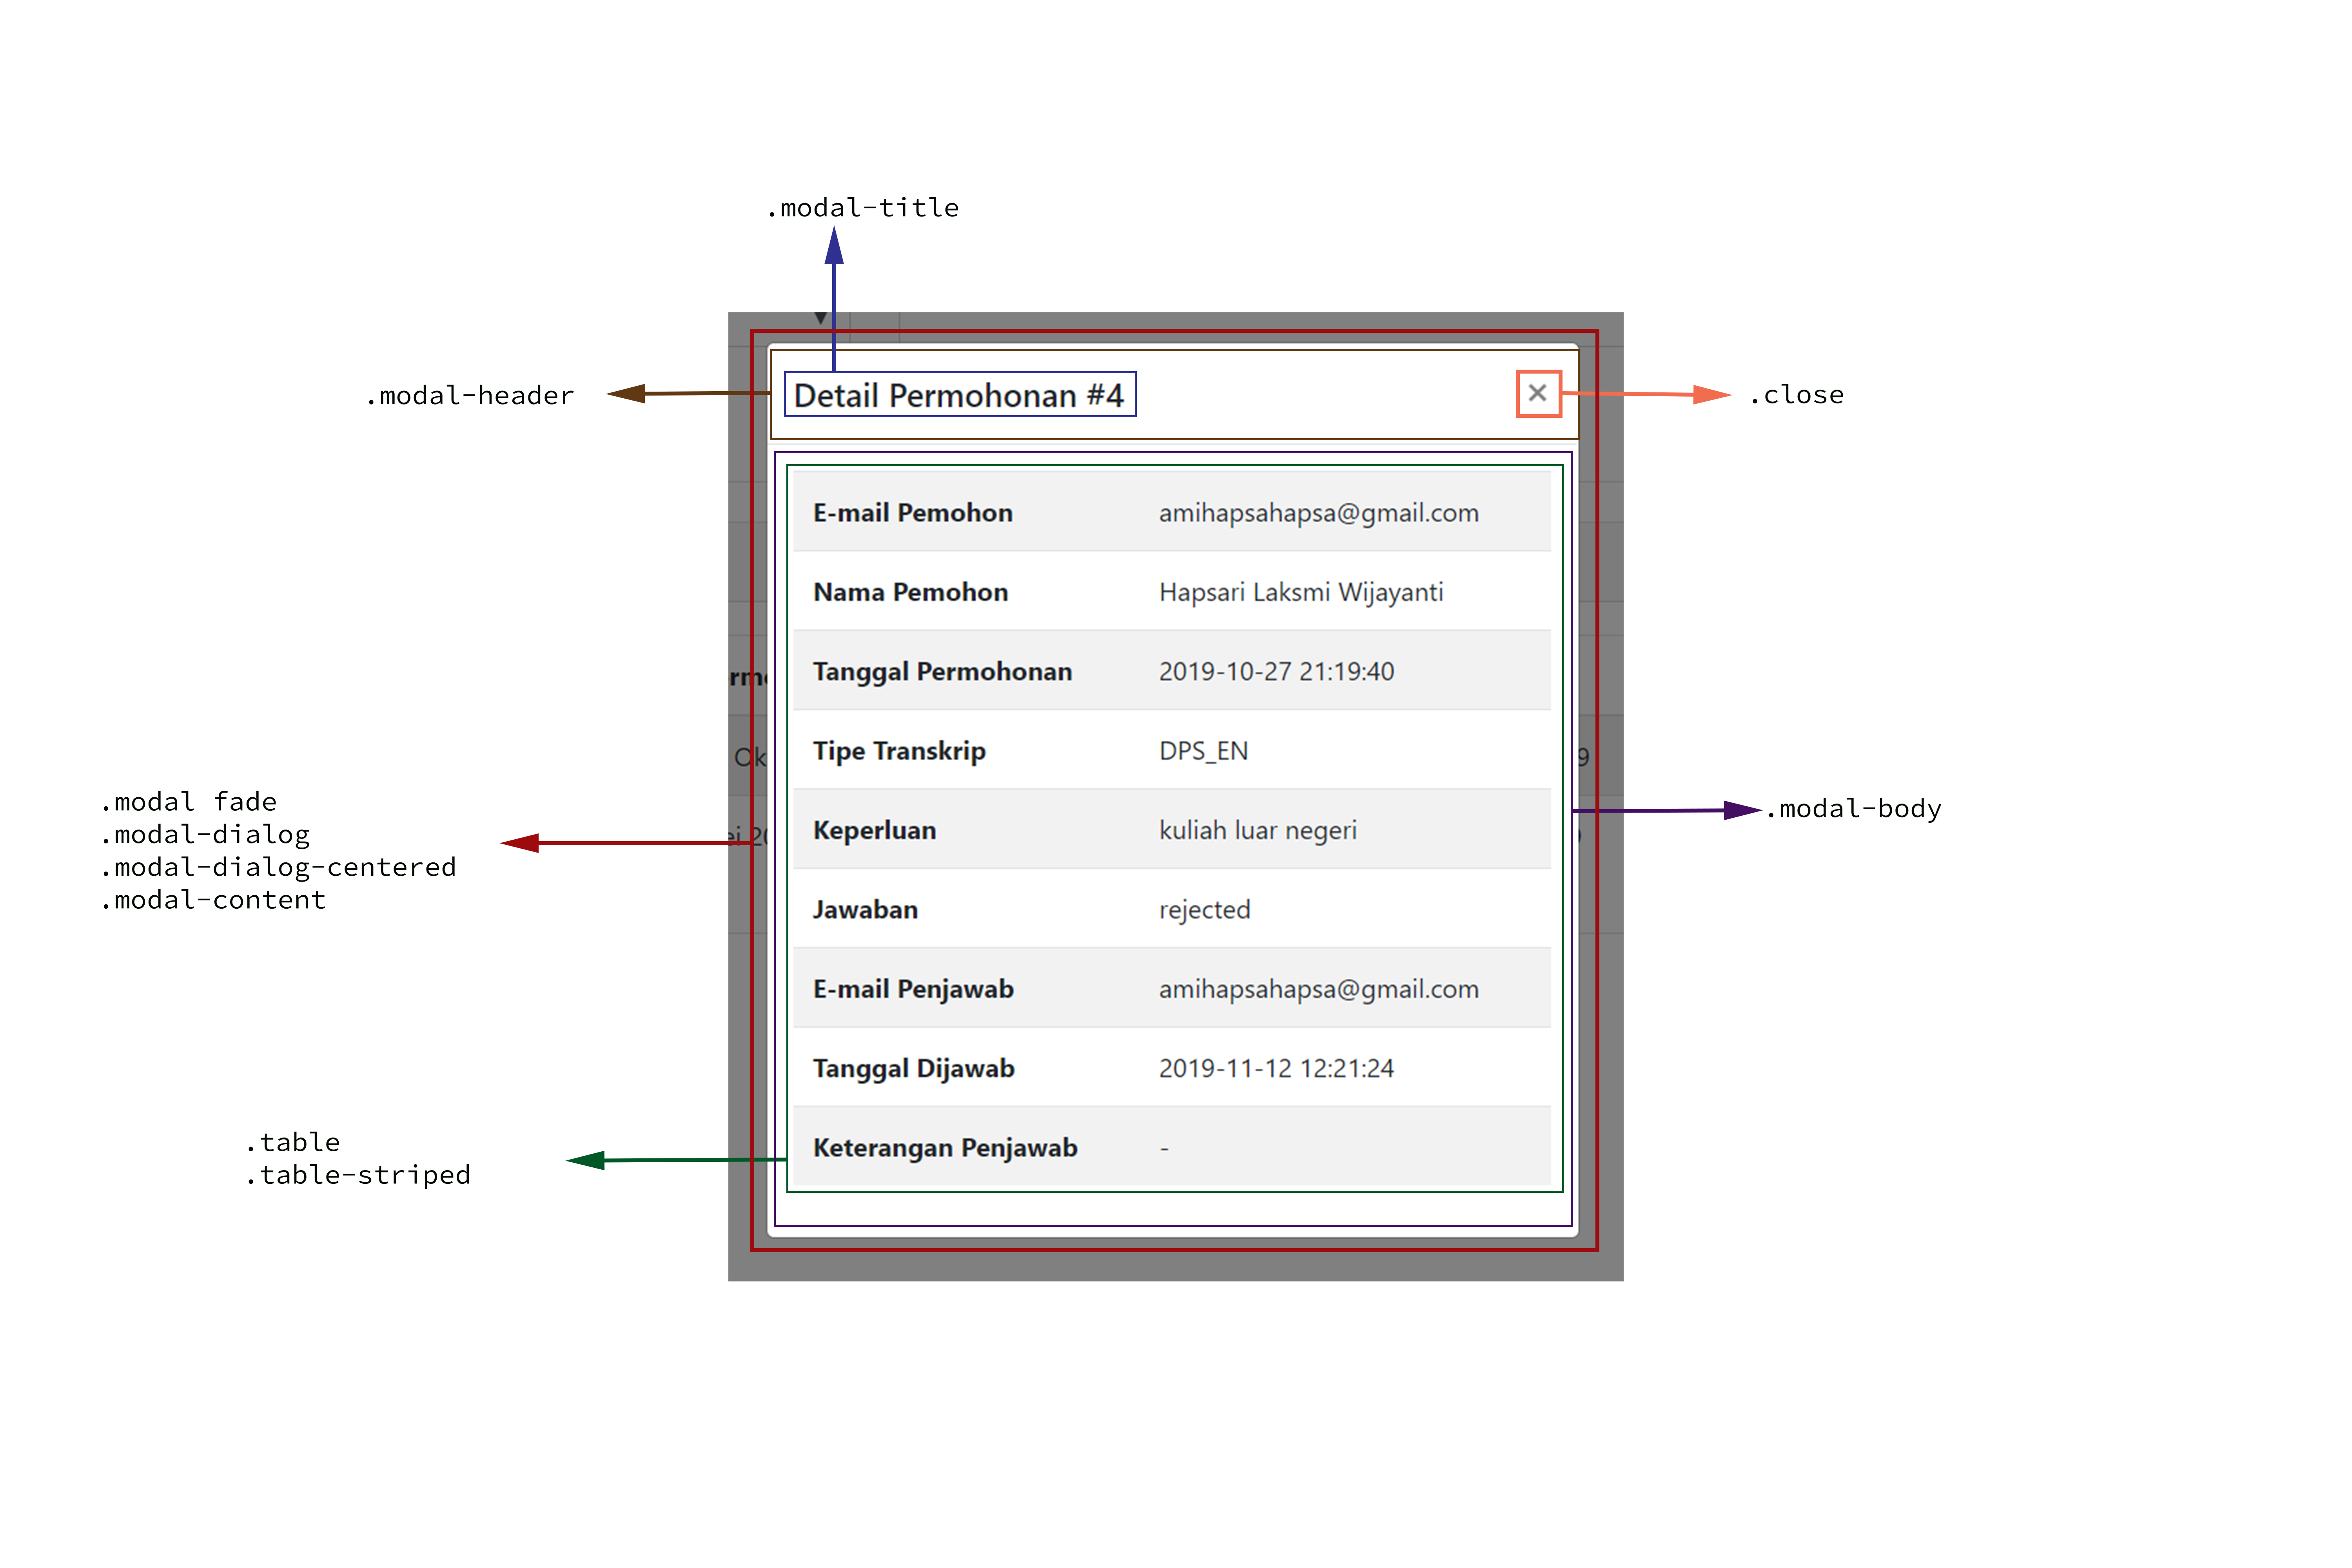
\includegraphics[width=0.6\textwidth,height=\textheight,keepaspectratio]{bootstrap/konversi_modal_lihat_cetak_transkrip.png}  
	\caption{Konversi modal lihat permintaan cetak transkrip.} 
	\label{fig:konversiLihatPermintaanCetakTranskrip}
\end{figure}

\noindent Perbandingan penggunaan kelas pada Foundation 6 dan Bootstrap 4 pada modal lihat permintaan cetak transkrip tertera pada tabel ~\ref{table:konversiLihatPermintaanCetakTranskrip}.\\

\begin{table}[H]
	\caption{Tabel konversi pada modal lihat permintaan cetak transkrip.}
	\begin{tabular}{| p{0.35\textwidth} | p{0.27\textwidth} | p{0.27\textwidth} |} 
		\hline
		\textbf{Jenis Komponen} & \textbf{Foundation 6} & \textbf{Bootstrap 4}  \\ [0.5ex] 
		\hline	
		Modal & \texttt{.reveal data-reveal} & \texttt{.modal-fade} \newline \texttt{.modal-dialog} \newline \texttt{.modal-dialog-centered} \newline \texttt{.modal-content} \\
		Judul modal & - & \texttt{modal-title}\\
		\hline
		Isi modal & - & \texttt{modal-body}\\
		\hline
		Tutup modal & \texttt{.close-button} \newline \texttt{data-close} \newline \texttt{aria-label} & \texttt{.close}\\
		\hline	
		Tabel & \texttt{.stack} & \texttt{.table} \newline \texttt{.table-striped} \\[1ex]
		\hline
	\end{tabular}
	\label{table:konversiLihatPermintaanCetakTranskrip}
\end{table}

\subsection{Halaman Manajemen Cetak Transkrip}

\noindent Gambar ~\ref{fig:konversiManajemenCetakTranskrip} menjelaskan komponen dalam website beserta penamaan kelas untuk Bootstrap 4 pada halaman manajemen cetak transkrip.\\
\subsubsection{Halaman Utama}
\begin{figure} [H]
	\centering  
	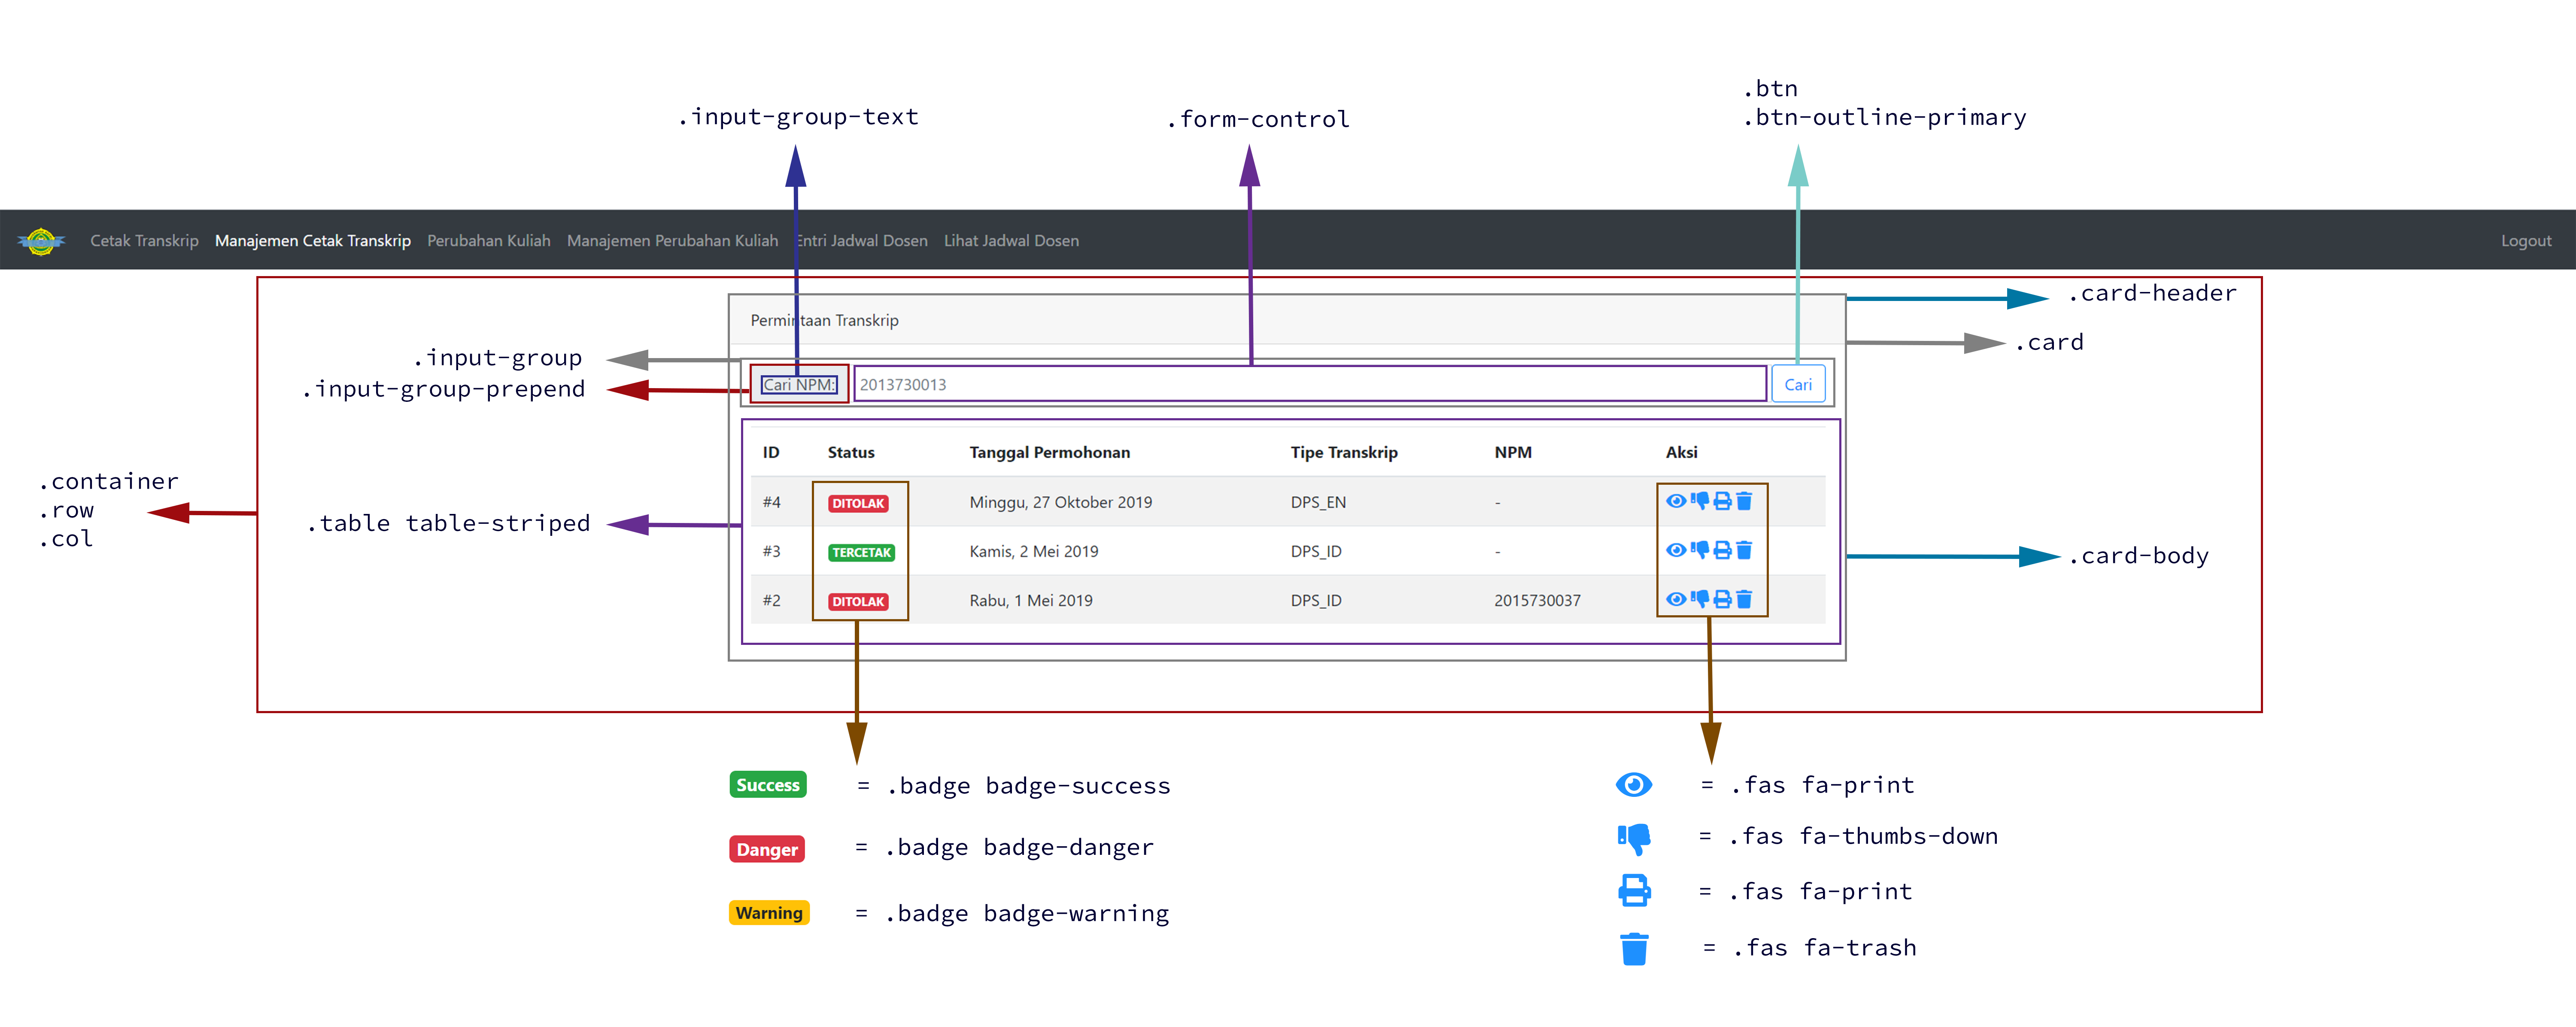
\includegraphics[width=\textwidth,height=\textheight,keepaspectratio]{bootstrap/konversi_tampilan_manajemen_cetak_transkrip.png}
	\caption{Konversi manajemen cetak transkrip.} 
	\label{fig:konversiManajemenCetakTranskrip}
\end{figure}

\begin{table}[H]
	\caption{Tabel konversi pada halaman manajemen cetak transkrip.}
	\begin{tabular}{| p{0.35\textwidth} | p{0.27\textwidth} | p{0.27\textwidth} |} 
		\hline
		\textbf{Jenis Komponen} & \textbf{Foundation 6} & \textbf{Bootstrap 4}  \\ [0.5ex] 
		\hline	
		Sistem Grid & \texttt{.row} &   \texttt{.container} \\ 
		\hline	
		Border untuk konten & \texttt{.callout} &  \texttt{.card} \newline \texttt{.card-header} \newline \texttt{.card-body} \\
		\hline
		Kolom & \texttt{.column} &  \texttt{.col} \\	
		\hline	
		Label berwarna hijau & \texttt{.label success} &  \texttt{.badge badge-success} \\
		\hline	
		Label berwarna merah &\texttt{.label alert} & \texttt{.badge badge-danger}  \\
		\hline	
		Label berwarna abu & \texttt{.label secondary} & \texttt{.badge badge-secondary}  \\
		\hline	
	\end{tabular}
\end{table}

\begin{table}[H] \ContinuedFloat
	\caption{Tabel konversi pada halaman manajemen cetak transkrip (cont.).}
	\begin{tabular}{| p{0.35\textwidth} | p{0.27\textwidth} | p{0.27\textwidth} |} 
		\hline
		\textbf{Jenis Komponen} & \textbf{Foundation 6} & \textbf{Bootstrap 4}  \\ [0.5ex] 
		\hline	
		Ikon bentuk \textit{eye} & \texttt{.fi-eye} &  \texttt{.fas fa-eye} \\	
		\hline	
		Ikon bentuk \textit{down} & \texttt{.fi-dislike} &  \texttt{.fas fa-thumbs-down} \\	
		\hline
		Ikon bentuk \textit{print} & \texttt{.fi-print} &  \texttt{.fas fa-prin}t \\	
		\hline
		Ikon bentuk \textit{trash} & \texttt{.fi-trash} &  \texttt{.fas fa-trash} \\	
		\hline
		Tabel & \texttt{.stack} & \texttt{.table table-striped}  \\
		\hline	
		\textit{Input Group} & \texttt{.input-group} \newline \texttt{.input-group-label} \newline \texttt{.input-group-field} \newline \texttt{.input-group-button} & \texttt{.input-group-append} \newline \texttt{.input-group-text} \newline \texttt{.form-control} \newline \texttt{.btn btn-primary} \\[1ex]
		\hline	
	\end{tabular}
	\label{table:konversiManajemenCetakTranskrip}
\end{table}

\subsubsection{Modal: Lihat, Tolak, Print, Hapus}
\noindent Gambar ~\ref{fig:konversiModalManajemenCetakTranskrip} menjelaskan komponen dalam website beserta penamaan kelas untuk Bootstrap 4 pada modal-modal  halaman manajemen cetak transkrip.\\
\begin{figure} [H]	
	\centering
	\begin{subfigure}[b]{0.45\linewidth}   
		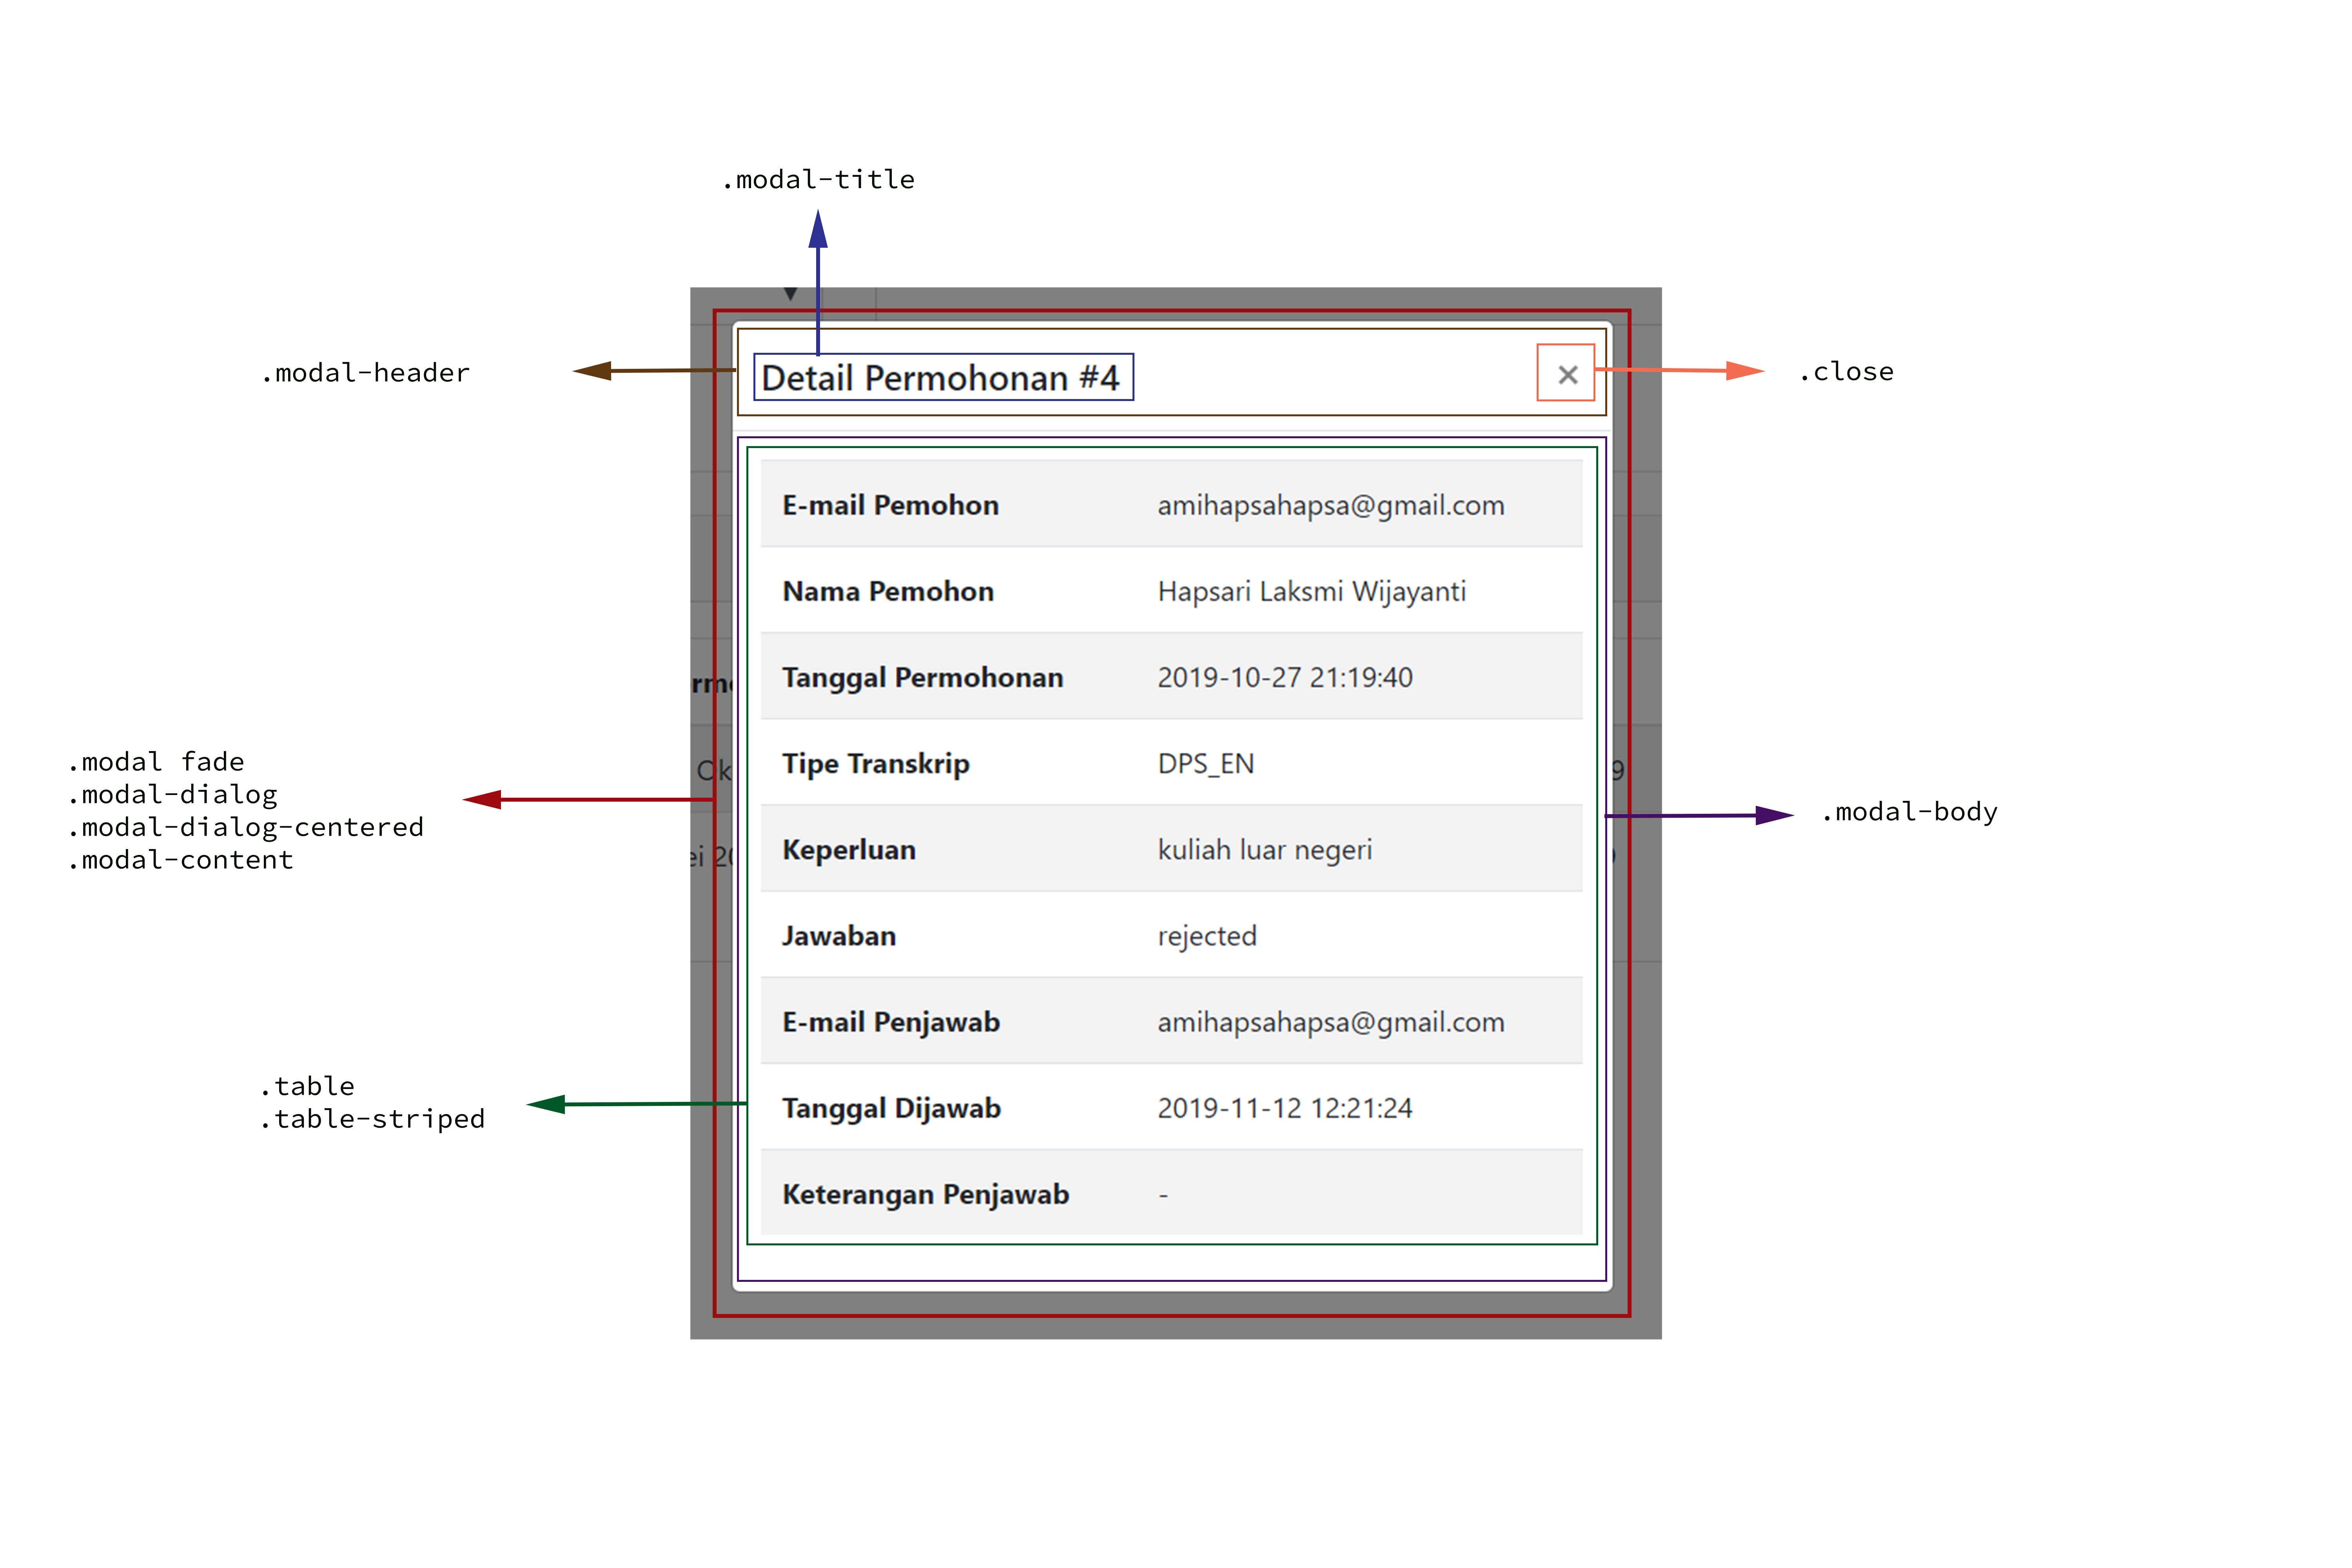
\includegraphics[width=\textwidth,height=\textheight,keepaspectratio]{bootstrap/konversi_modal_lihat_manajemen_cetak_transkrip.png}
		\caption{Modal lihat.} 
	\end{subfigure}
	\begin{subfigure}[b]{0.45\linewidth} 
		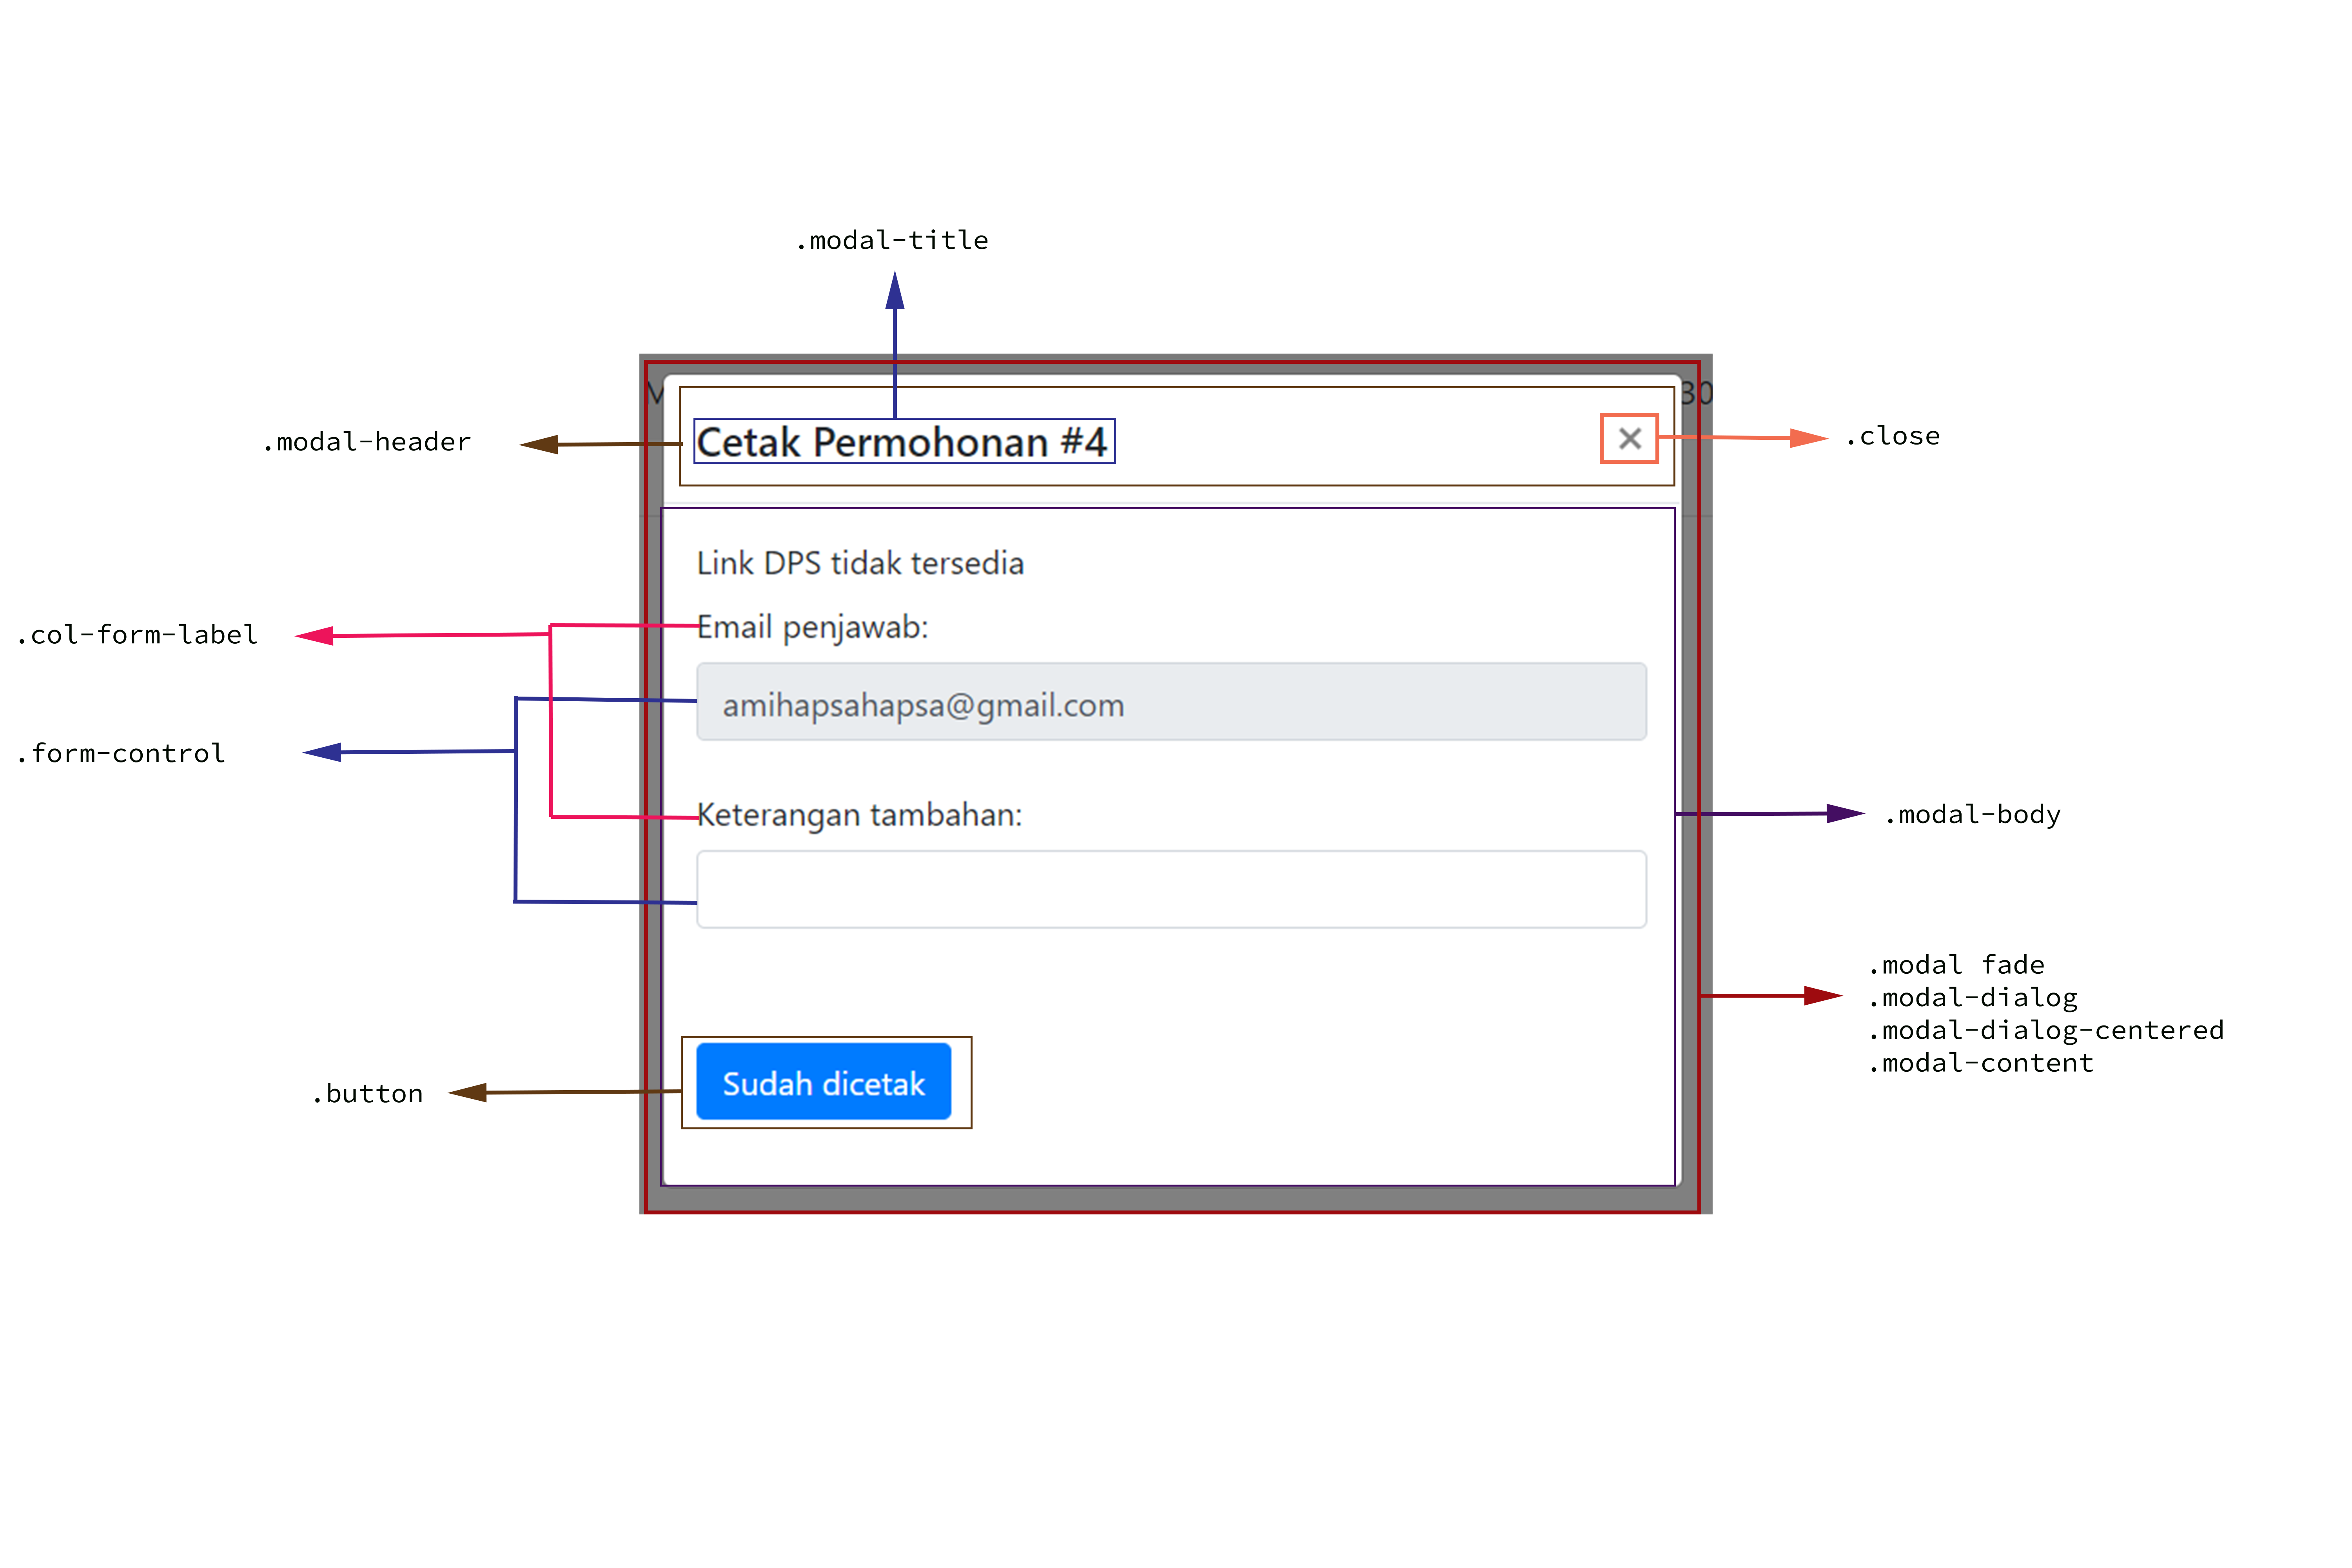
\includegraphics[width=\textwidth,height=\textheight,keepaspectratio]{bootstrap/konversi_modal_print_manajemen_cetak_transkrip.png}
		\caption{Modal print.} 
	\end{subfigure}
\end{figure} 
\begin{figure} [H]
	\centering
	\ContinuedFloat
	\begin{subfigure}[b]{0.45\linewidth}  
		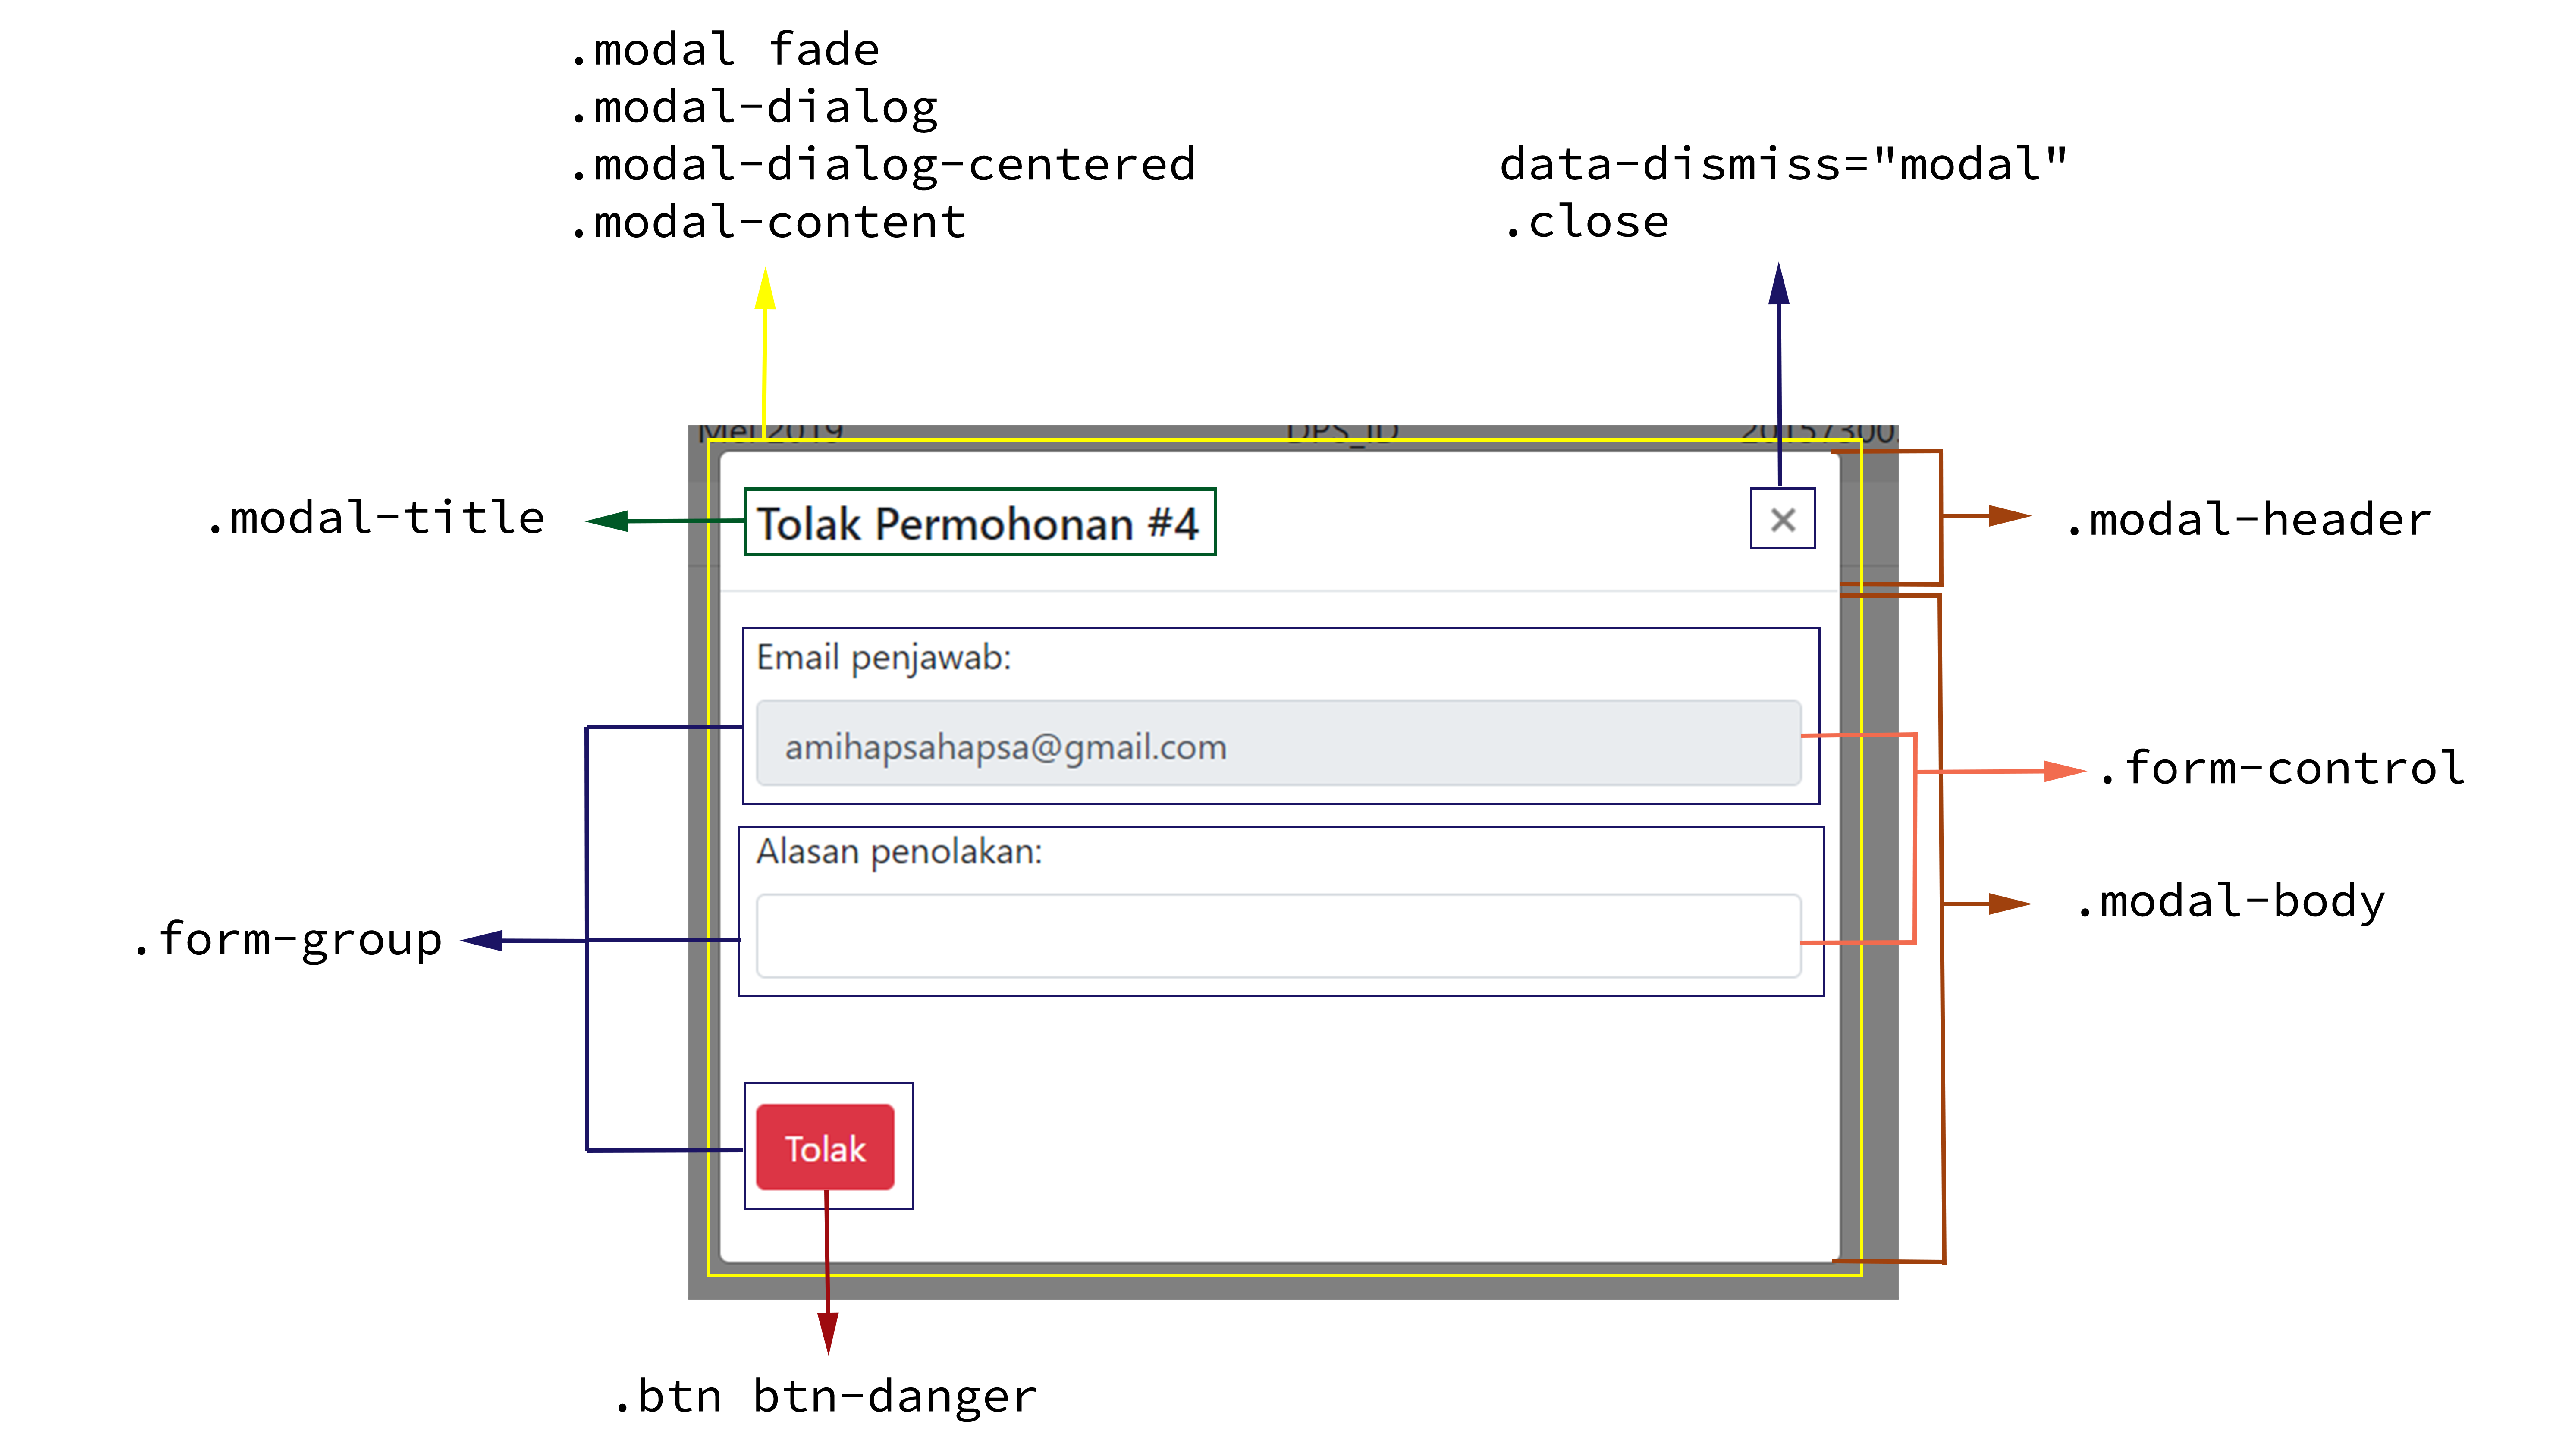
\includegraphics[width=\textwidth,height=\textheight,keepaspectratio]{bootstrap/konversi_modal_dislike_manajemen_cetak_transkrip.png}
		\caption{Modal tolak.} 
	\end{subfigure}
	\begin{subfigure}[b]{0.45\linewidth}  
		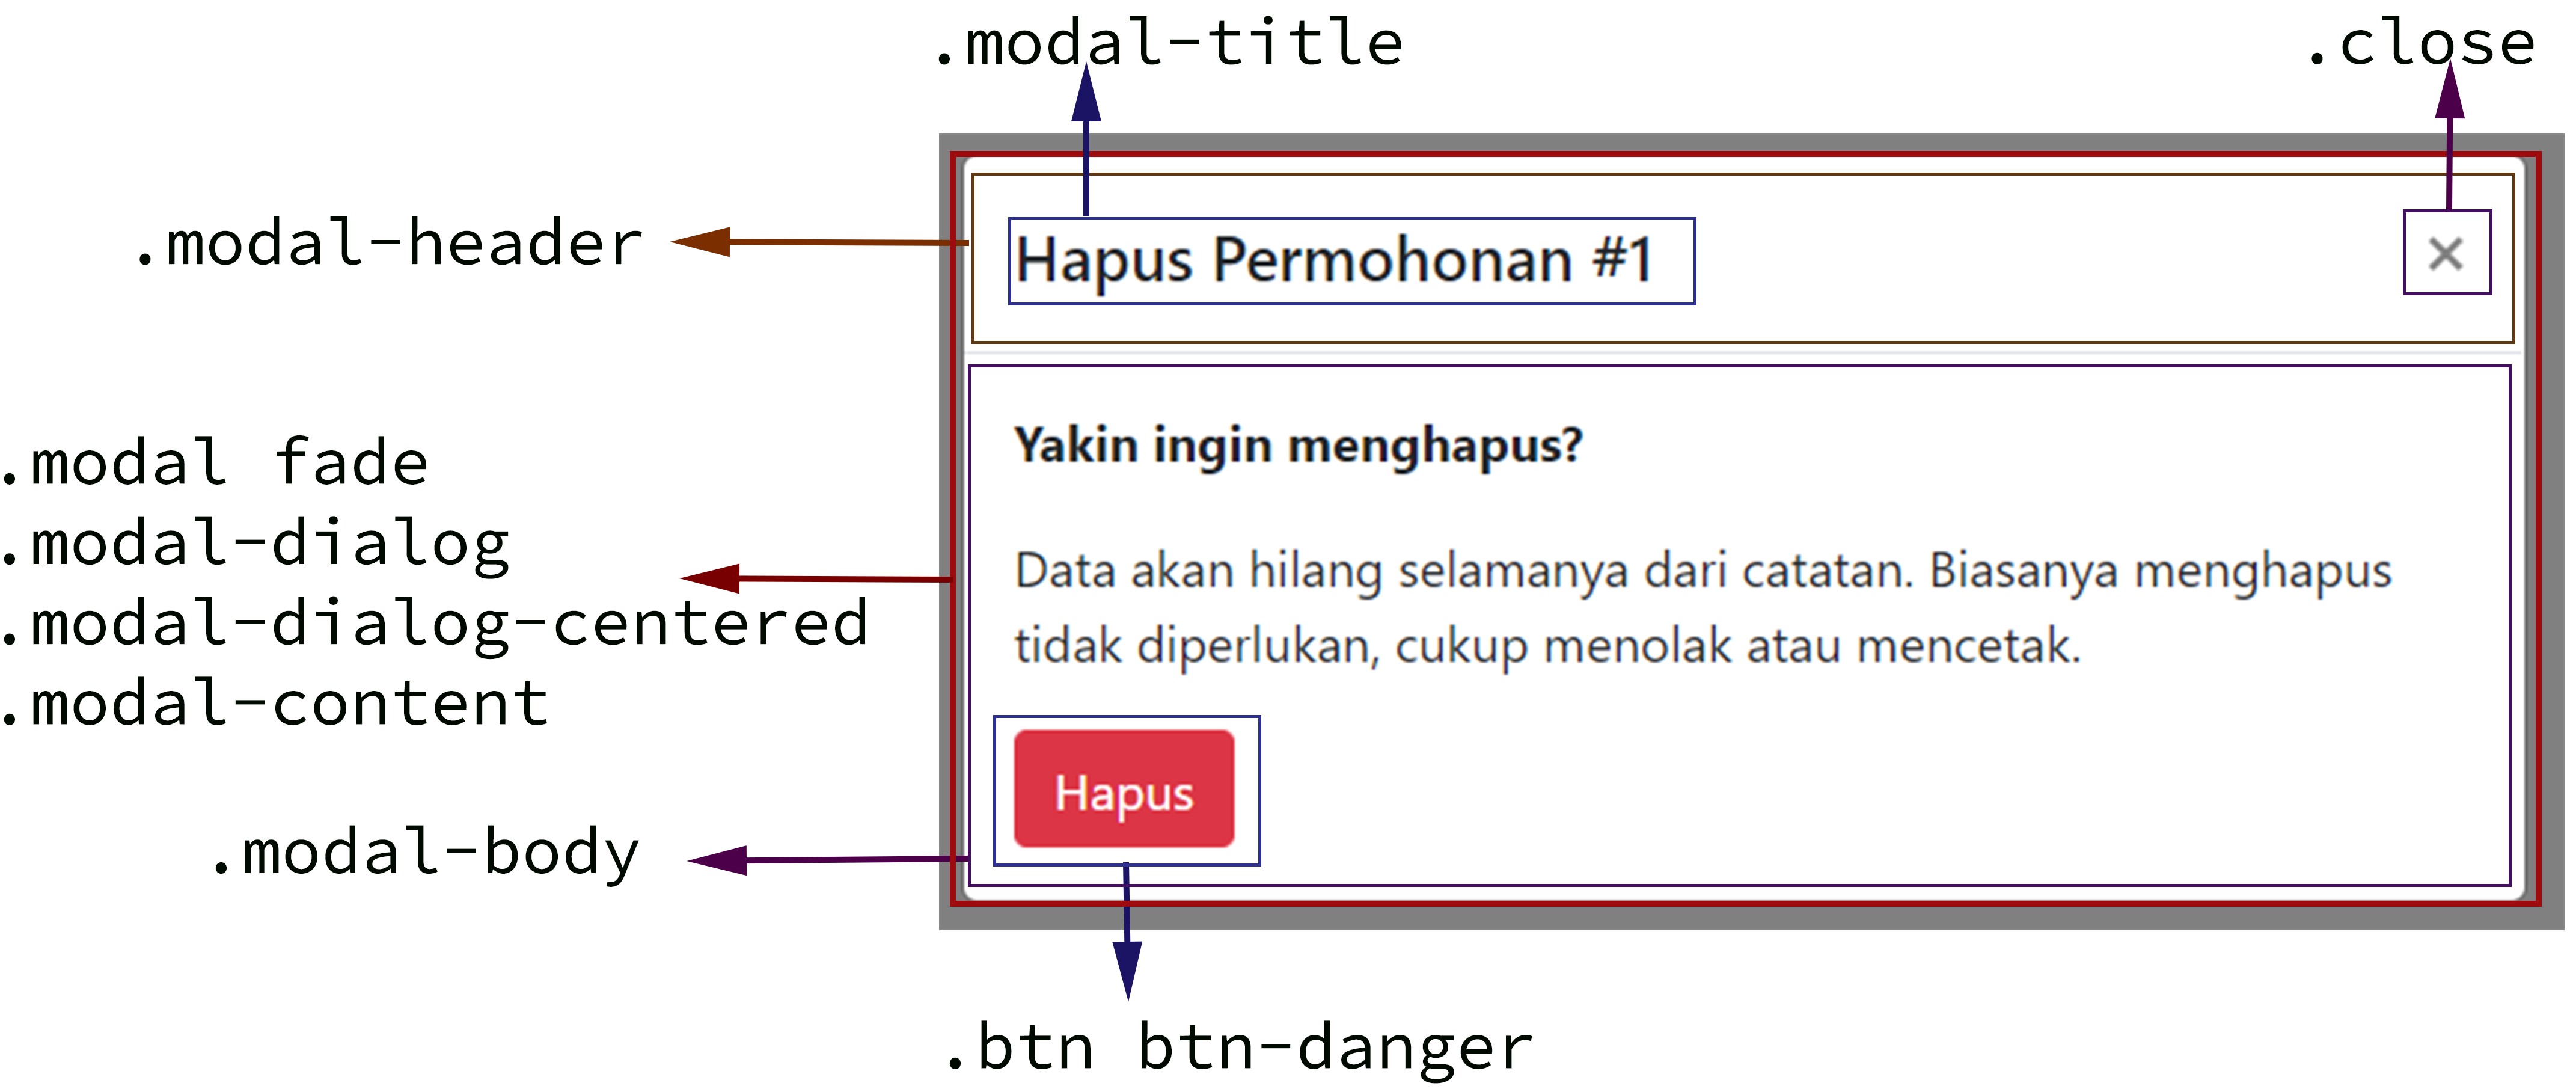
\includegraphics[width=\textwidth,height=\textheight,keepaspectratio]{bootstrap/konversi_modal_trash_manajemen_cetak_transkrip.png}
		\caption{Modal hapus.} 
	\end{subfigure}
	\caption{Konversi modal pada halaman manajemen cetak transkrip.}
	\label{fig:konversiModalManajemenCetakTranskrip}
\end{figure}

\noindent Penjabaran kelas - kelas yang digunakan ada pada tabel ~\ref{table:konversiModalManajemenCetakTranskrip}
\begin{table}[H]
	\caption{Tabel konversi modal pada manajemen cetak transkrip.}
	\begin{tabular}{| p{0.35\textwidth} | p{0.27\textwidth} | p{0.27\textwidth} |} 
		\hline
		\textbf{Jenis Komponen} & \textbf{Foundation 6} & \textbf{Bootstrap 4}  \\ [0.5ex] 
		\hline	
		Modal & \texttt{.reveal data-reveal} & \texttt{.modal-fade} \newline \texttt{.modal-dialog} \newline \texttt{.modal-dialog-centered} \newline \texttt{.modal-content} \\
		\hline
		Judul modal & - & \texttt{modal-title}\\
		\hline
		Isi modal & - & \texttt{modal-body}\\
		\hline
		Tutup modal & \texttt{.close-button} \newline \texttt{data-close} \newline \texttt{aria-label} & \texttt{.close}\\
		\hline	
		Tabel & \texttt{.stack} & \texttt{.table} \newline \texttt{.table-striped} \\	[1ex]
		\hline 		
	\end{tabular}
\end{table}

\begin{table}[H] \ContinuedFloat
	\caption{Tabel konversi modal pada manajemen cetak transkrip(cont.).}
	\begin{tabular}{| p{0.35\textwidth} | p{0.27\textwidth} | p{0.27\textwidth} |} 
		\hline
		\textbf{Jenis Komponen} & \textbf{Foundation 6} & \textbf{Bootstrap 4}  \\ [0.5ex] 
		\hline	
		Judul \textit{form} & - & \texttt{.col-form-label}\\
		\hline
		\textit{Field form} & \texttt{.input-group-field} & \texttt{.form-control}\\
		\hline
		\textit{Form group} & \texttt{.input-group} & \texttt{.form-group}\\
		\hline
		Tombol berwarna biru & \texttt{.button} & \texttt{.btn-primary}  \\
		\hline
		Tombol berwarna merah & \texttt{.alert button} & \texttt{.btn btn-danger} \\[1ex]
		\hline
	\end{tabular}
	\label{table:konversiModalManajemenCetakTranskrip}
\end{table}

\subsection{Halaman Permintaan Perubahan Kuliah}
\subsubsection{Halaman Utama}
\noindent Gambar ~\ref{fig:konversiPermintaanPerubahanKuliah} menjelaskan komponen dalam website beserta penamaan kelas untuk Bootstrap 4 pada halaman permintaan perubahan kuliah.\\
\begin{figure} [H]
	\centering  
	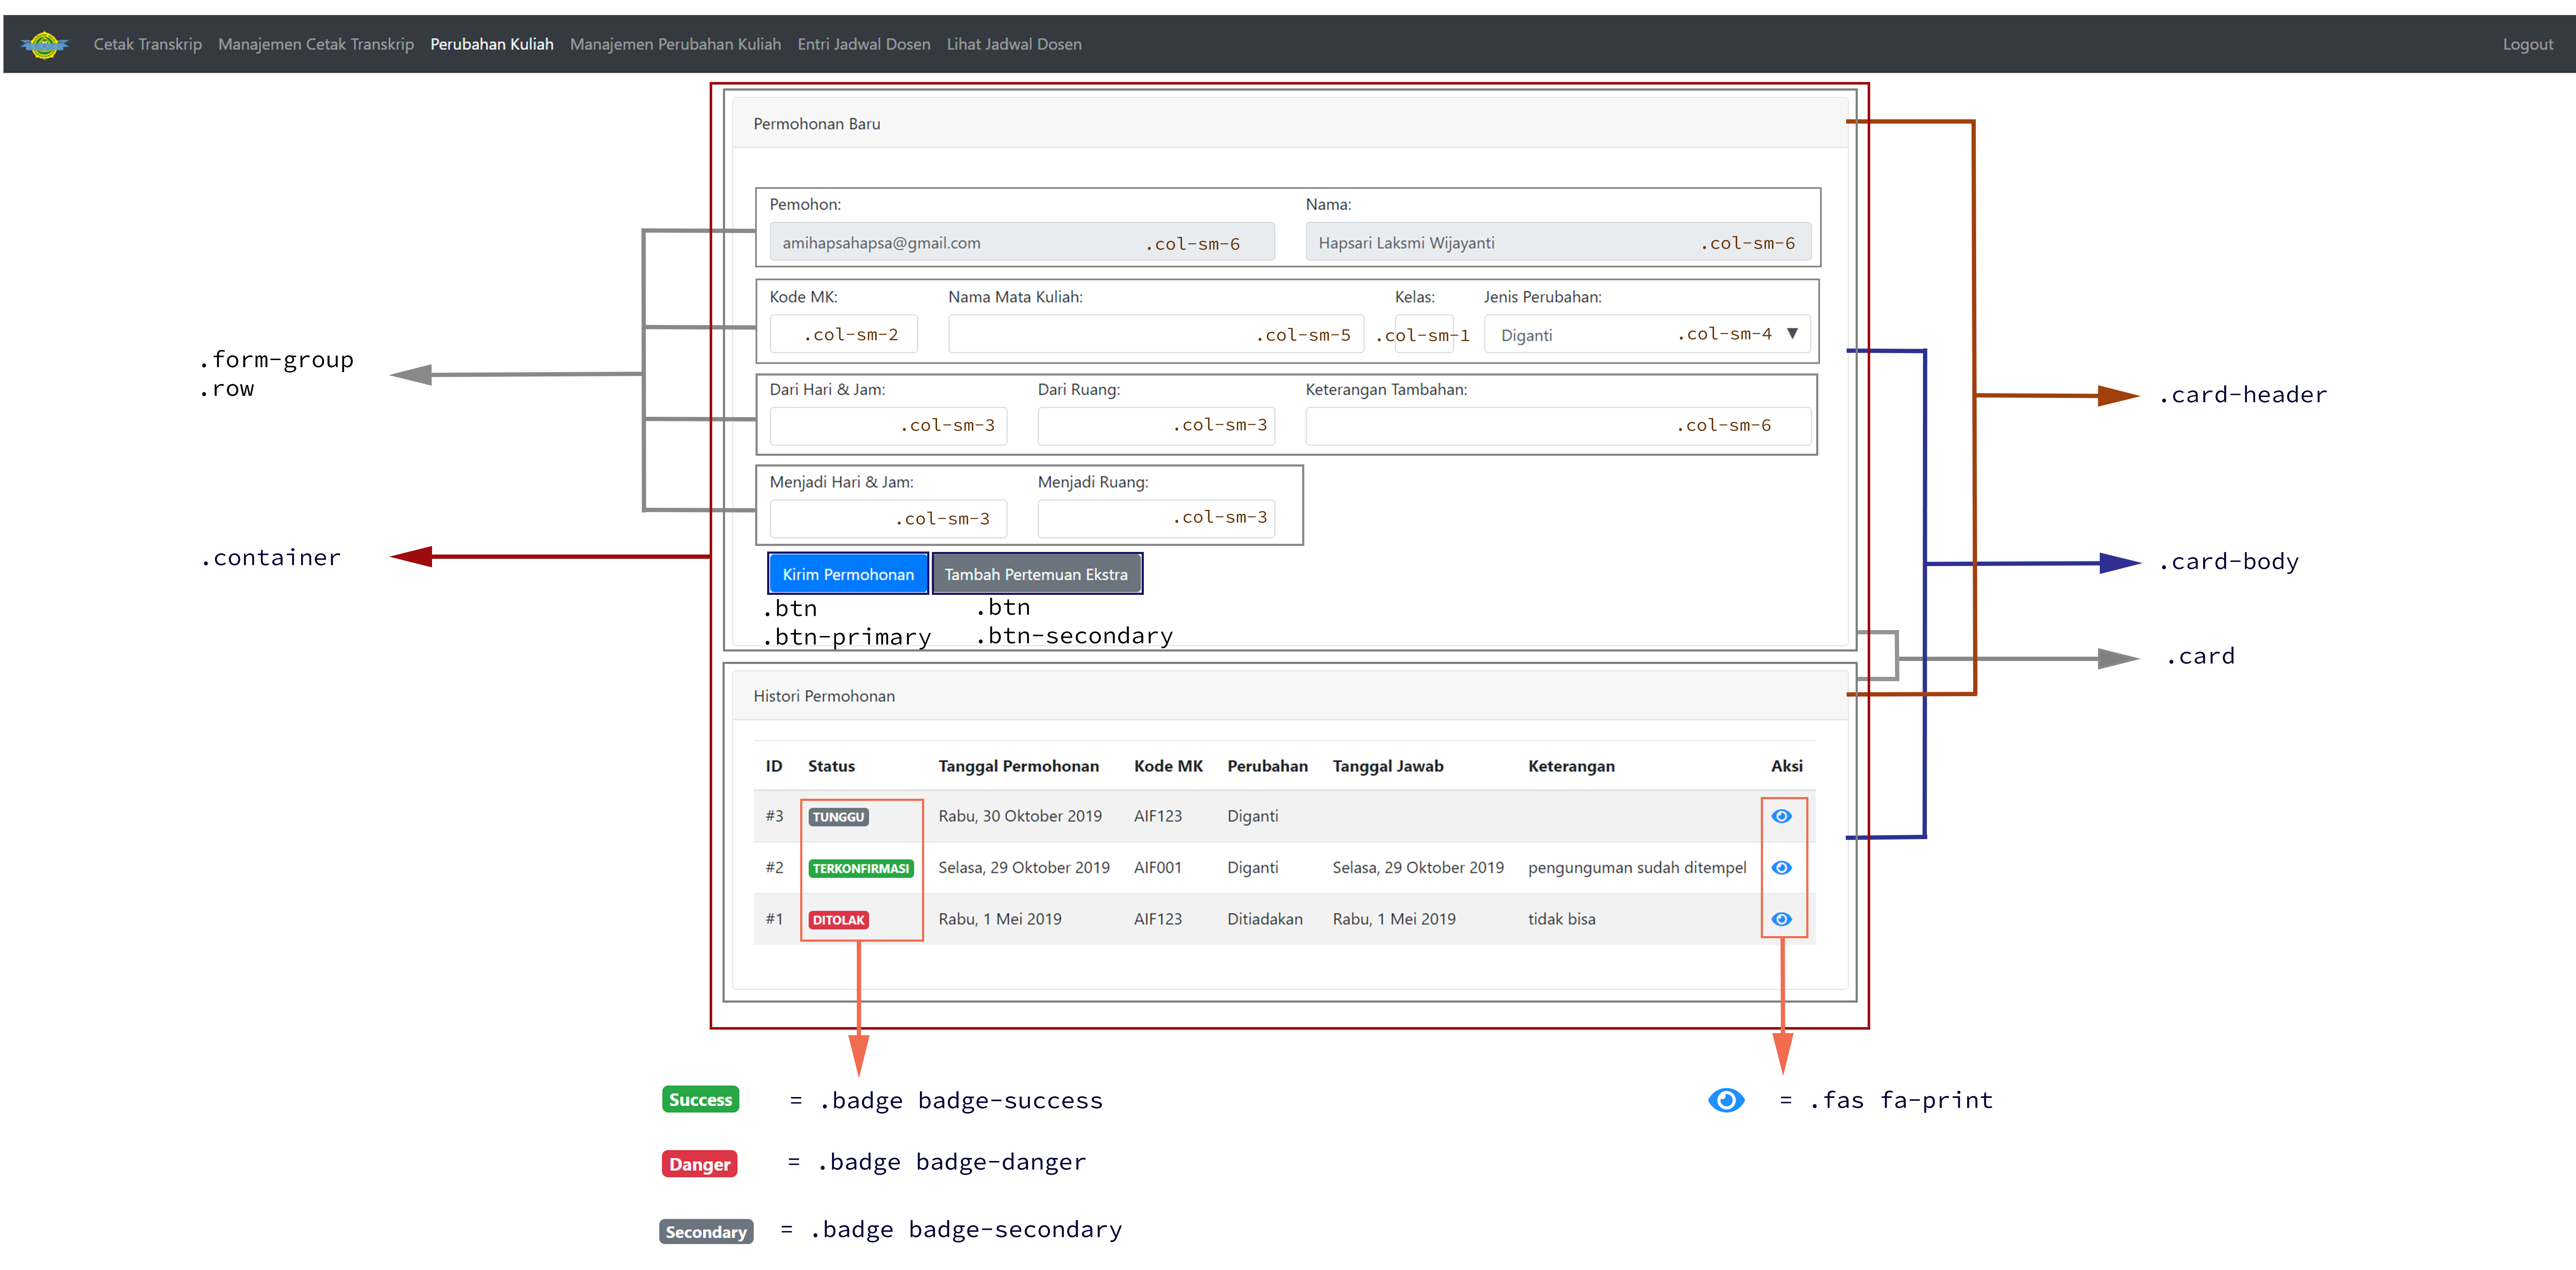
\includegraphics[width=\textwidth,height=\textheight,keepaspectratio]{bootstrap/konversi_tampilan_perubahan_kuliah.png}
	\caption{Konversi halaman permintaan perubahan kuliah.}
	\label{fig:konversiPermintaanPerubahanKuliah}
\end{figure}

\noindent Perbandingan penggunaan kelas pada Foundation 6 dan Bootstrap 4 pada halaman permintaan perubahan kuliah tertera pada tabel ~\ref{table:konversiPermintaanPerubahanKuliah}.\\
\begin{table}[H]
	\caption{Tabel konversi pada halaman permintaan perubahan kuliah.}
	\begin{tabular}{| p{0.35\textwidth} | p{0.27\textwidth} | p{0.27\textwidth} |} 
		\hline
		\textbf{Jenis Komponen} & \textbf{Foundation 6} & \textbf{Bootstrap 4}  \\ [0.5ex] 
		\hline	
		Sistem Grid & \texttt{.row} &   \texttt{.container} \\ 
		\hline	
		Border untuk konten & \texttt{.callout} &  \texttt{.card}  \\
		&& \texttt{.card-header}\\
		&& \texttt{.card-body}\\
		\hline	
		Ukuran grid & \texttt{.small-*} &  \texttt{.col-sm-*} \\
		\hline
		Kolom & \texttt{.column} &  \texttt{.col} \\	
		\hline	
		Tombol berwarna biru & \texttt{.button} &  \texttt{.btn btn-primary}\\
		\hline	
		Label berwarna hijau & \texttt{.label success } & \texttt{.badge badge-success} \\
		\hline	
		Label berwarna merah & \texttt{.label alert} & \texttt{.badge badge-danger}  \\
		\hline	
		Label berwarna abu & \texttt{.label secondary} & \texttt{.badge badge-secondary}  \\
		\hline	
		Ikon bentuk mata & \texttt{.fi-eye} &  \texttt{.fas fa-eye} \\	
		\hline	
		Tabel & \texttt{.stack} & \texttt{.table table-striped}  \\
		\hline	
		Nama \textit{form} & - & \texttt{.col-form-label}  \\ 
		\hline	
		Input \textit{form} & - & \texttt{.form-control}  \\ [1ex] 
		\hline
	\end{tabular}
	\label{table:konversiPermintaanPerubahanKuliah}
\end{table}

\subsubsection{Modal: Lihat}

\noindent Gambar ~\ref{fig:konversiLihatPermintaanPerubahanKuliah} menjelaskan komponen dalam website beserta penamaan kelas untuk Bootstrap 4 pada modal lihat permintaan perubahan kuliah.\\
\begin{figure} [H]
	\centering  
	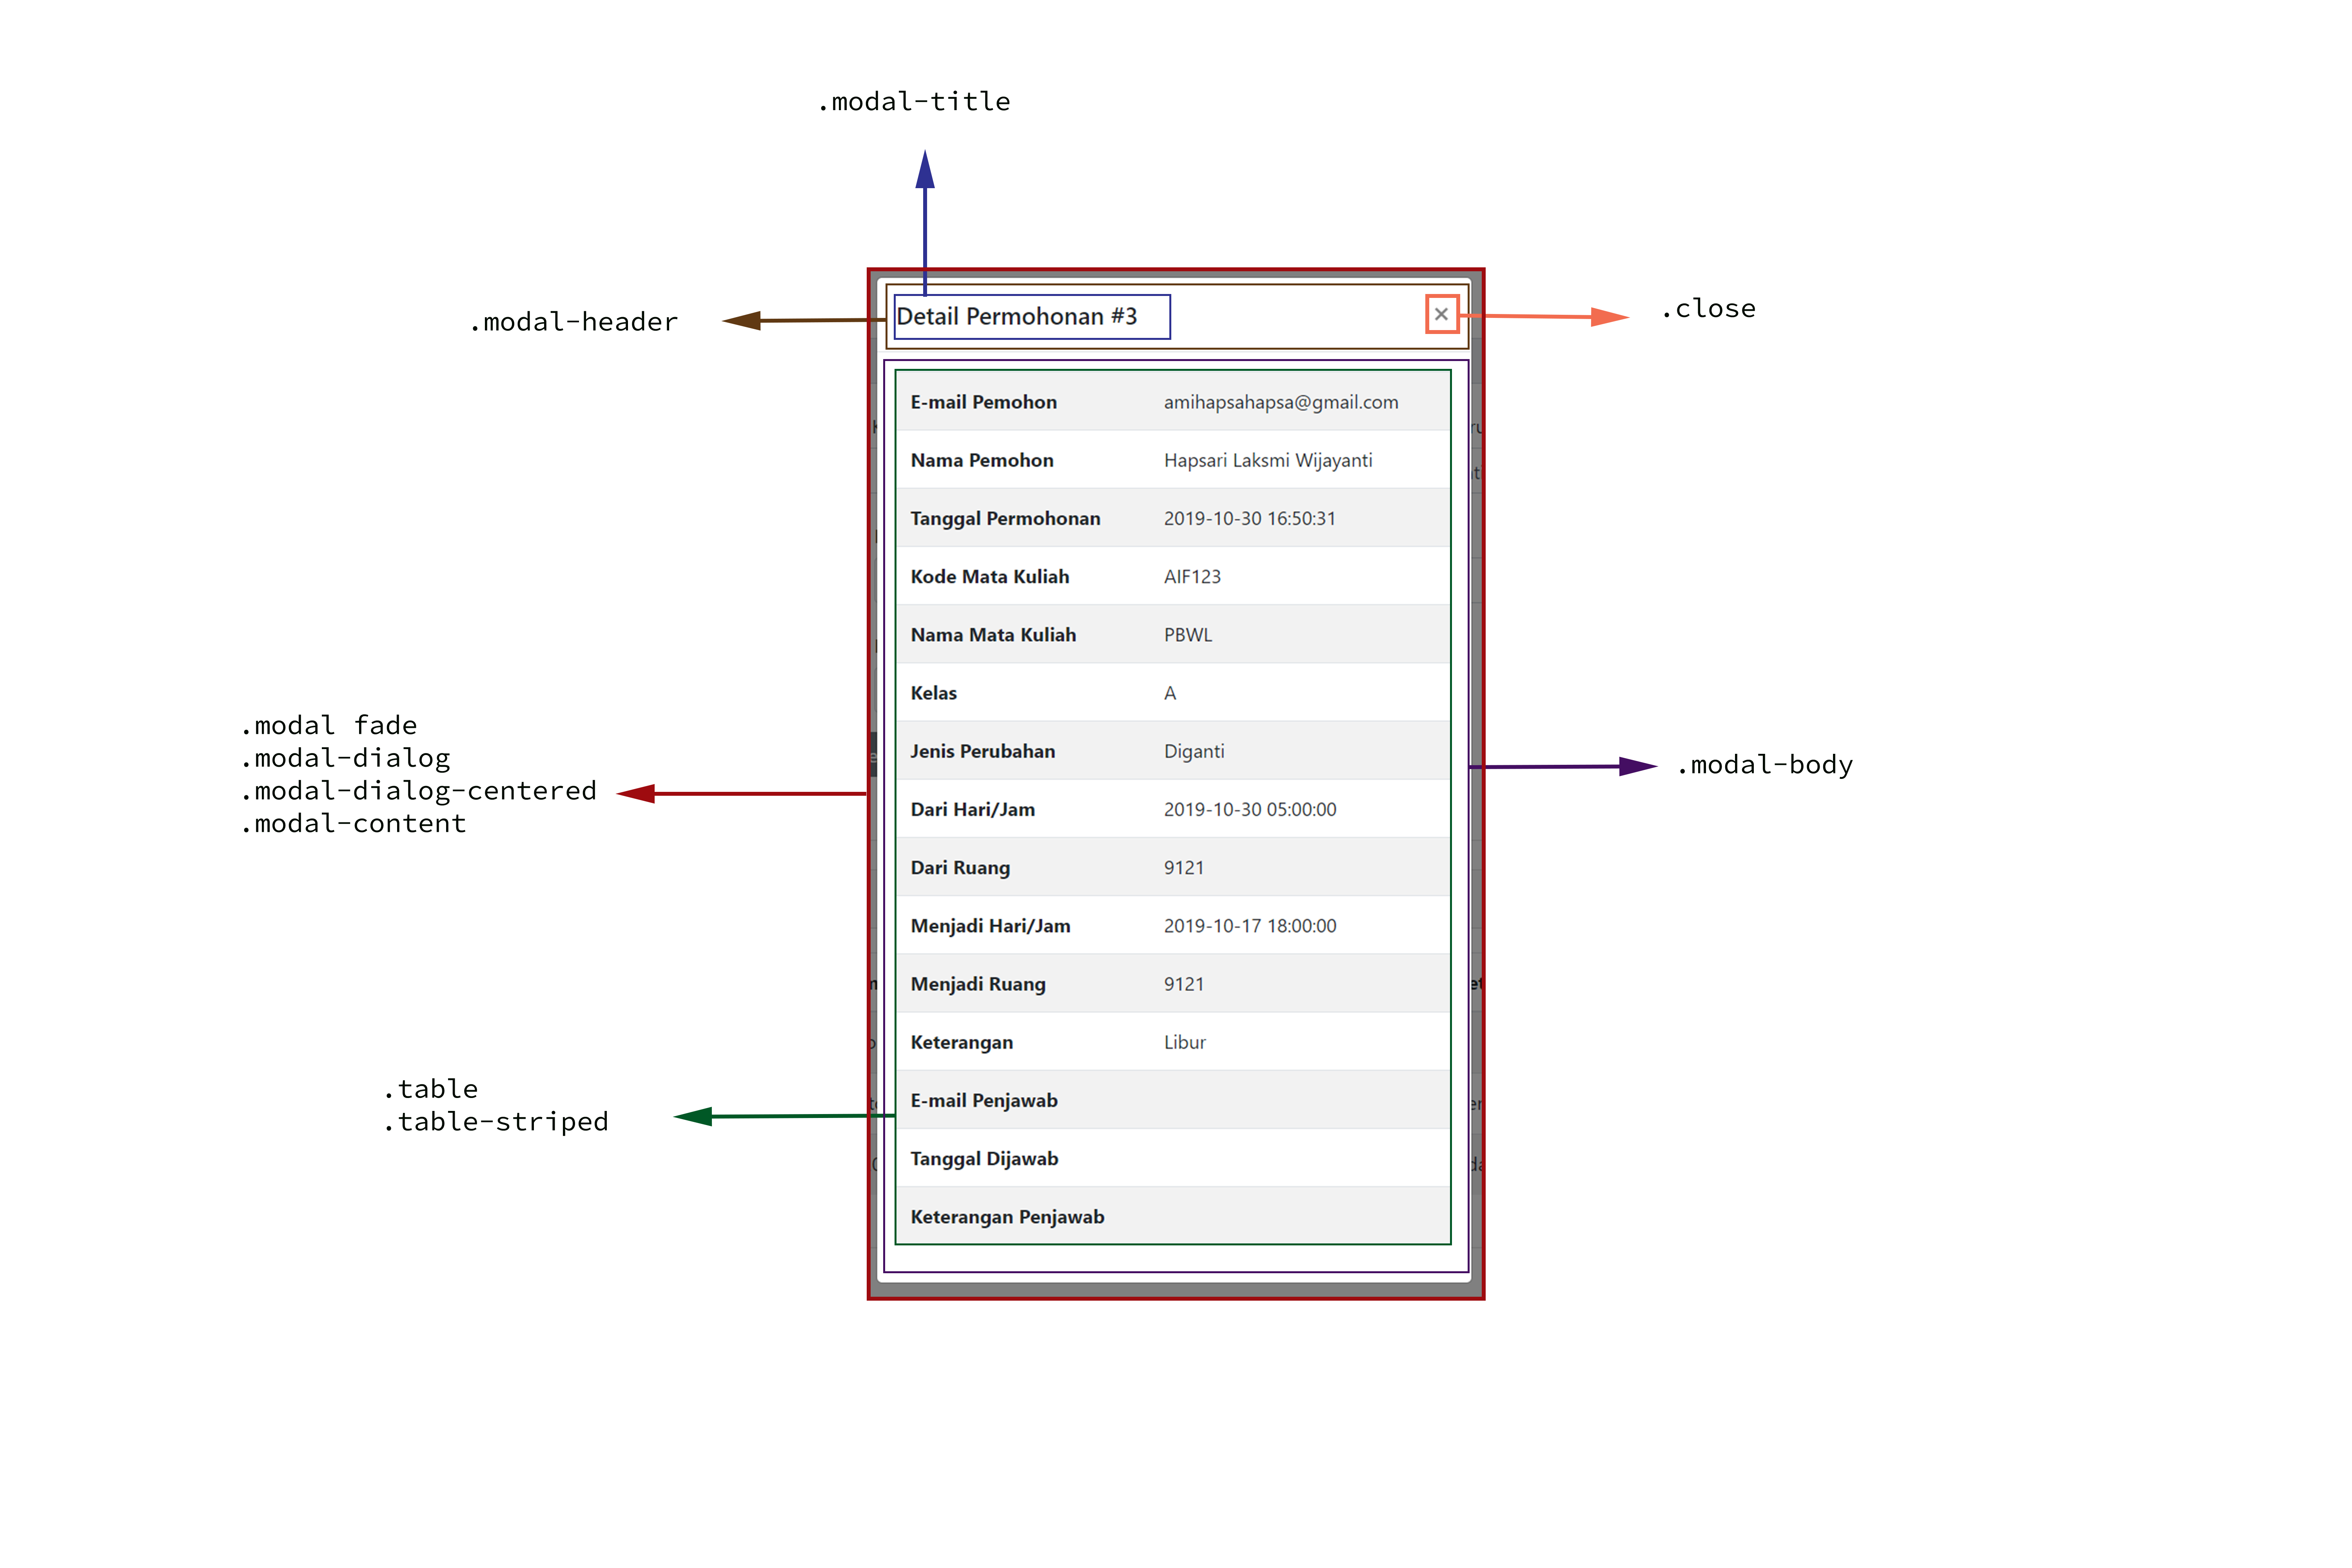
\includegraphics[width=0.4\textwidth,height=\textheight,keepaspectratio]{bootstrap/konversi_modal_lihat_perubahan_kuliah.png}
	\caption{Konversi modal lihat permintaan perubahan kuliah.}
	\label{fig:konversiLihatPermintaanPerubahanKuliah}
\end{figure}

\noindent Perbandingan penggunaan kelas pada Foundation 6 dan Bootstrap 4 pada modal lihat permintaan perubahan kuliah tertera pada tabel ~\ref{table:konversiLihatPermintaanPerubahanKuliah}.\\
\begin{table}[H]
	\caption{Tabel konversi pada modal lihat permintaan perubahan kuliah.}
	\begin{tabular}{| p{0.35\textwidth} | p{0.27\textwidth} | p{0.27\textwidth} |} 
		\hline
		\textbf{Jenis Komponen} & \textbf{Foundation 6} & \textbf{Bootstrap 4}  \\ [0.5ex] 
		\hline	
		Modal & \texttt{.reveal data-reveal} & \texttt{.modal-fade} \newline \texttt{.modal-dialog} \newline \texttt{.modal-dialog-centered} \newline \texttt{.modal-content} \\
		\hline
		Judul modal & - & \texttt{modal-title}\\
		\hline
		Isi modal & - & \texttt{modal-body}\\
		\hline
		Tutup modal & \texttt{.close-button} \newline \texttt{data-close} \newline \texttt{aria-label} & \texttt{.close}\\
		\hline	
		Tabel & \texttt{.stack} & \texttt{.table} \newline \texttt{.table-striped} \\[1ex]
		\hline
	\end{tabular}
	\label{table:konversiLihatPermintaanPerubahanKuliah}
\end{table}



\subsection{Halaman Manajemen Perubahan Kuliah}
\subsubsection{Halaman Utama}
\noindent Gambar ~\ref{fig:konversiManajemenPerubahanKuliah} menjelaskan komponen dalam website beserta penamaan kelas untuk Bootstrap 4 pada halaman manajemen perubahan kuliah.\\
\begin{figure} [H]
	\centering  
	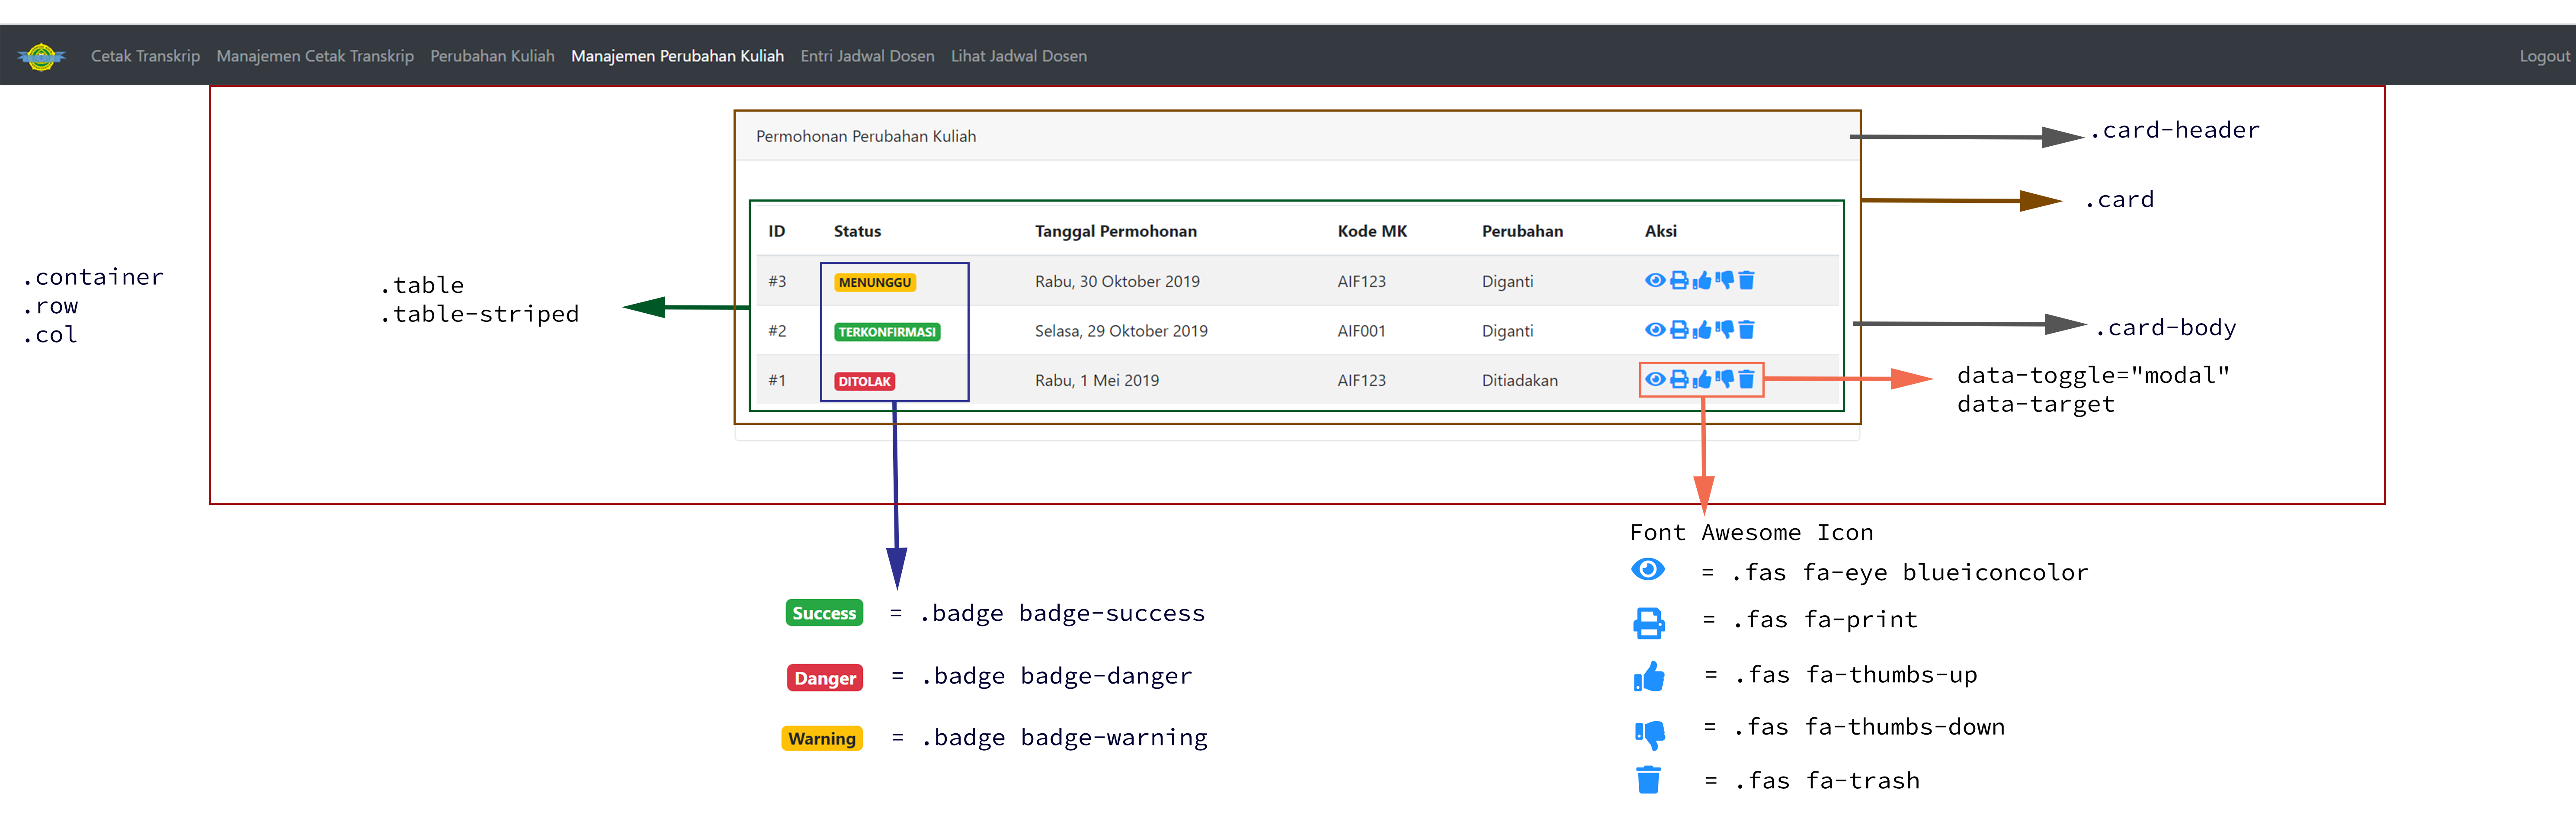
\includegraphics[width=\textwidth,height=\textheight,keepaspectratio]{bootstrap/konversi_tampilan_manajemen_perubahan_kuliah.png}
	\caption{Konversi halaman manajemen perubahan kuliah.}
	\label{fig:konversiManajemenPerubahanKuliah}
\end{figure}

\noindent Perbandingan penggunaan kelas pada Foundation 6 dan Bootstrap 4 pada halaman manajemen perubahan kuliah tertera pada tabel ~\ref{table:konversiManajemenPerubahanKuliah}.\\
\begin{table}[H]
	\caption{Tabel konversi pada halaman manajemen perubahan kuliah.}
	\begin{tabular}{| p{0.35\textwidth} | p{0.27\textwidth} | p{0.27\textwidth} |} 
		\hline
		\textbf{Jenis Komponen} & \textbf{Foundation 6} & \textbf{Bootstrap 4}  \\ [0.5ex] 
		\hline	
		Sistem Grid & \texttt{.row} &   \texttt{.container} \newline \texttt{.row} \newline \texttt{.col} \\ 
		\hline	
		Border untuk konten & \texttt{.callout} &  \texttt{.card} \newline \texttt{.card-header} \newline \texttt{.card-body} \\	
		\hline	
		Label berwarna hijau & \texttt{.label success} &  \texttt{.badge badge-success} \\
		\hline	
		Label berwarna merah &\texttt{.label alert} & \texttt{.badge badge-danger}  \\
		\hline	
		Label berwarna kuning & \texttt{.label warning} & \texttt{.badge badge-warning}  \\
		\hline	
		Link modal sesuai ID & \texttt{data-open} & \texttt{data-toggle} \newline \texttt{data-target} \\
		\hline
		Ikon bentuk \textit{eye} & \texttt{.fi-eye} &  \texttt{.fas fa-eye} \\	
		\hline	
		Ikon bentuk \textit{down} & \texttt{.fi-dislike} &  \texttt{.fas fa-thumbs-down} \\	
		\hline
		Ikon bentuk \textit{down} & \texttt{.fi-like} &  \texttt{.fas fa-thumbs-up} \\	
		\hline
		Ikon bentuk \textit{print} & \texttt{.fi-print} &  \texttt{.fas fa-print} \\	
		\hline
		Ikon bentuk \textit{trash} & \texttt{.fi-trash} &  \texttt{.fas fa-trash} \\	
		\hline
		Tabel & \texttt{.stack} & \texttt{.table table-striped}  \\
		\hline	
		\textit{Input Group} & \texttt{.input-group} \newline \texttt{.input-group-label} \newline \texttt{.input-group-field} \newline \texttt{.input-group-button} & \texttt{.input-group-append} \newline \texttt{.input-group-text} \newline \texttt{.form-control} \newline \texttt{.btn btn-primary} \\[1ex]
		\hline	
	\end{tabular}
	\label{table:konversiManajemenPerubahanKuliah}
\end{table}



\subsubsection{Modal: Lihat, Setujui, Tolak, Print, Hapus}

\noindent Gambar ~\ref{fig:konversiModalManajemenPerubahanKuliah} menjelaskan komponen dalam website beserta penamaan kelas untuk Bootstrap 4 pada halaman modal manajemen perubahan kuliah.\\
\begin{figure}[H]
	\centering
	\begin{subfigure}[b]{0.45\linewidth} 
		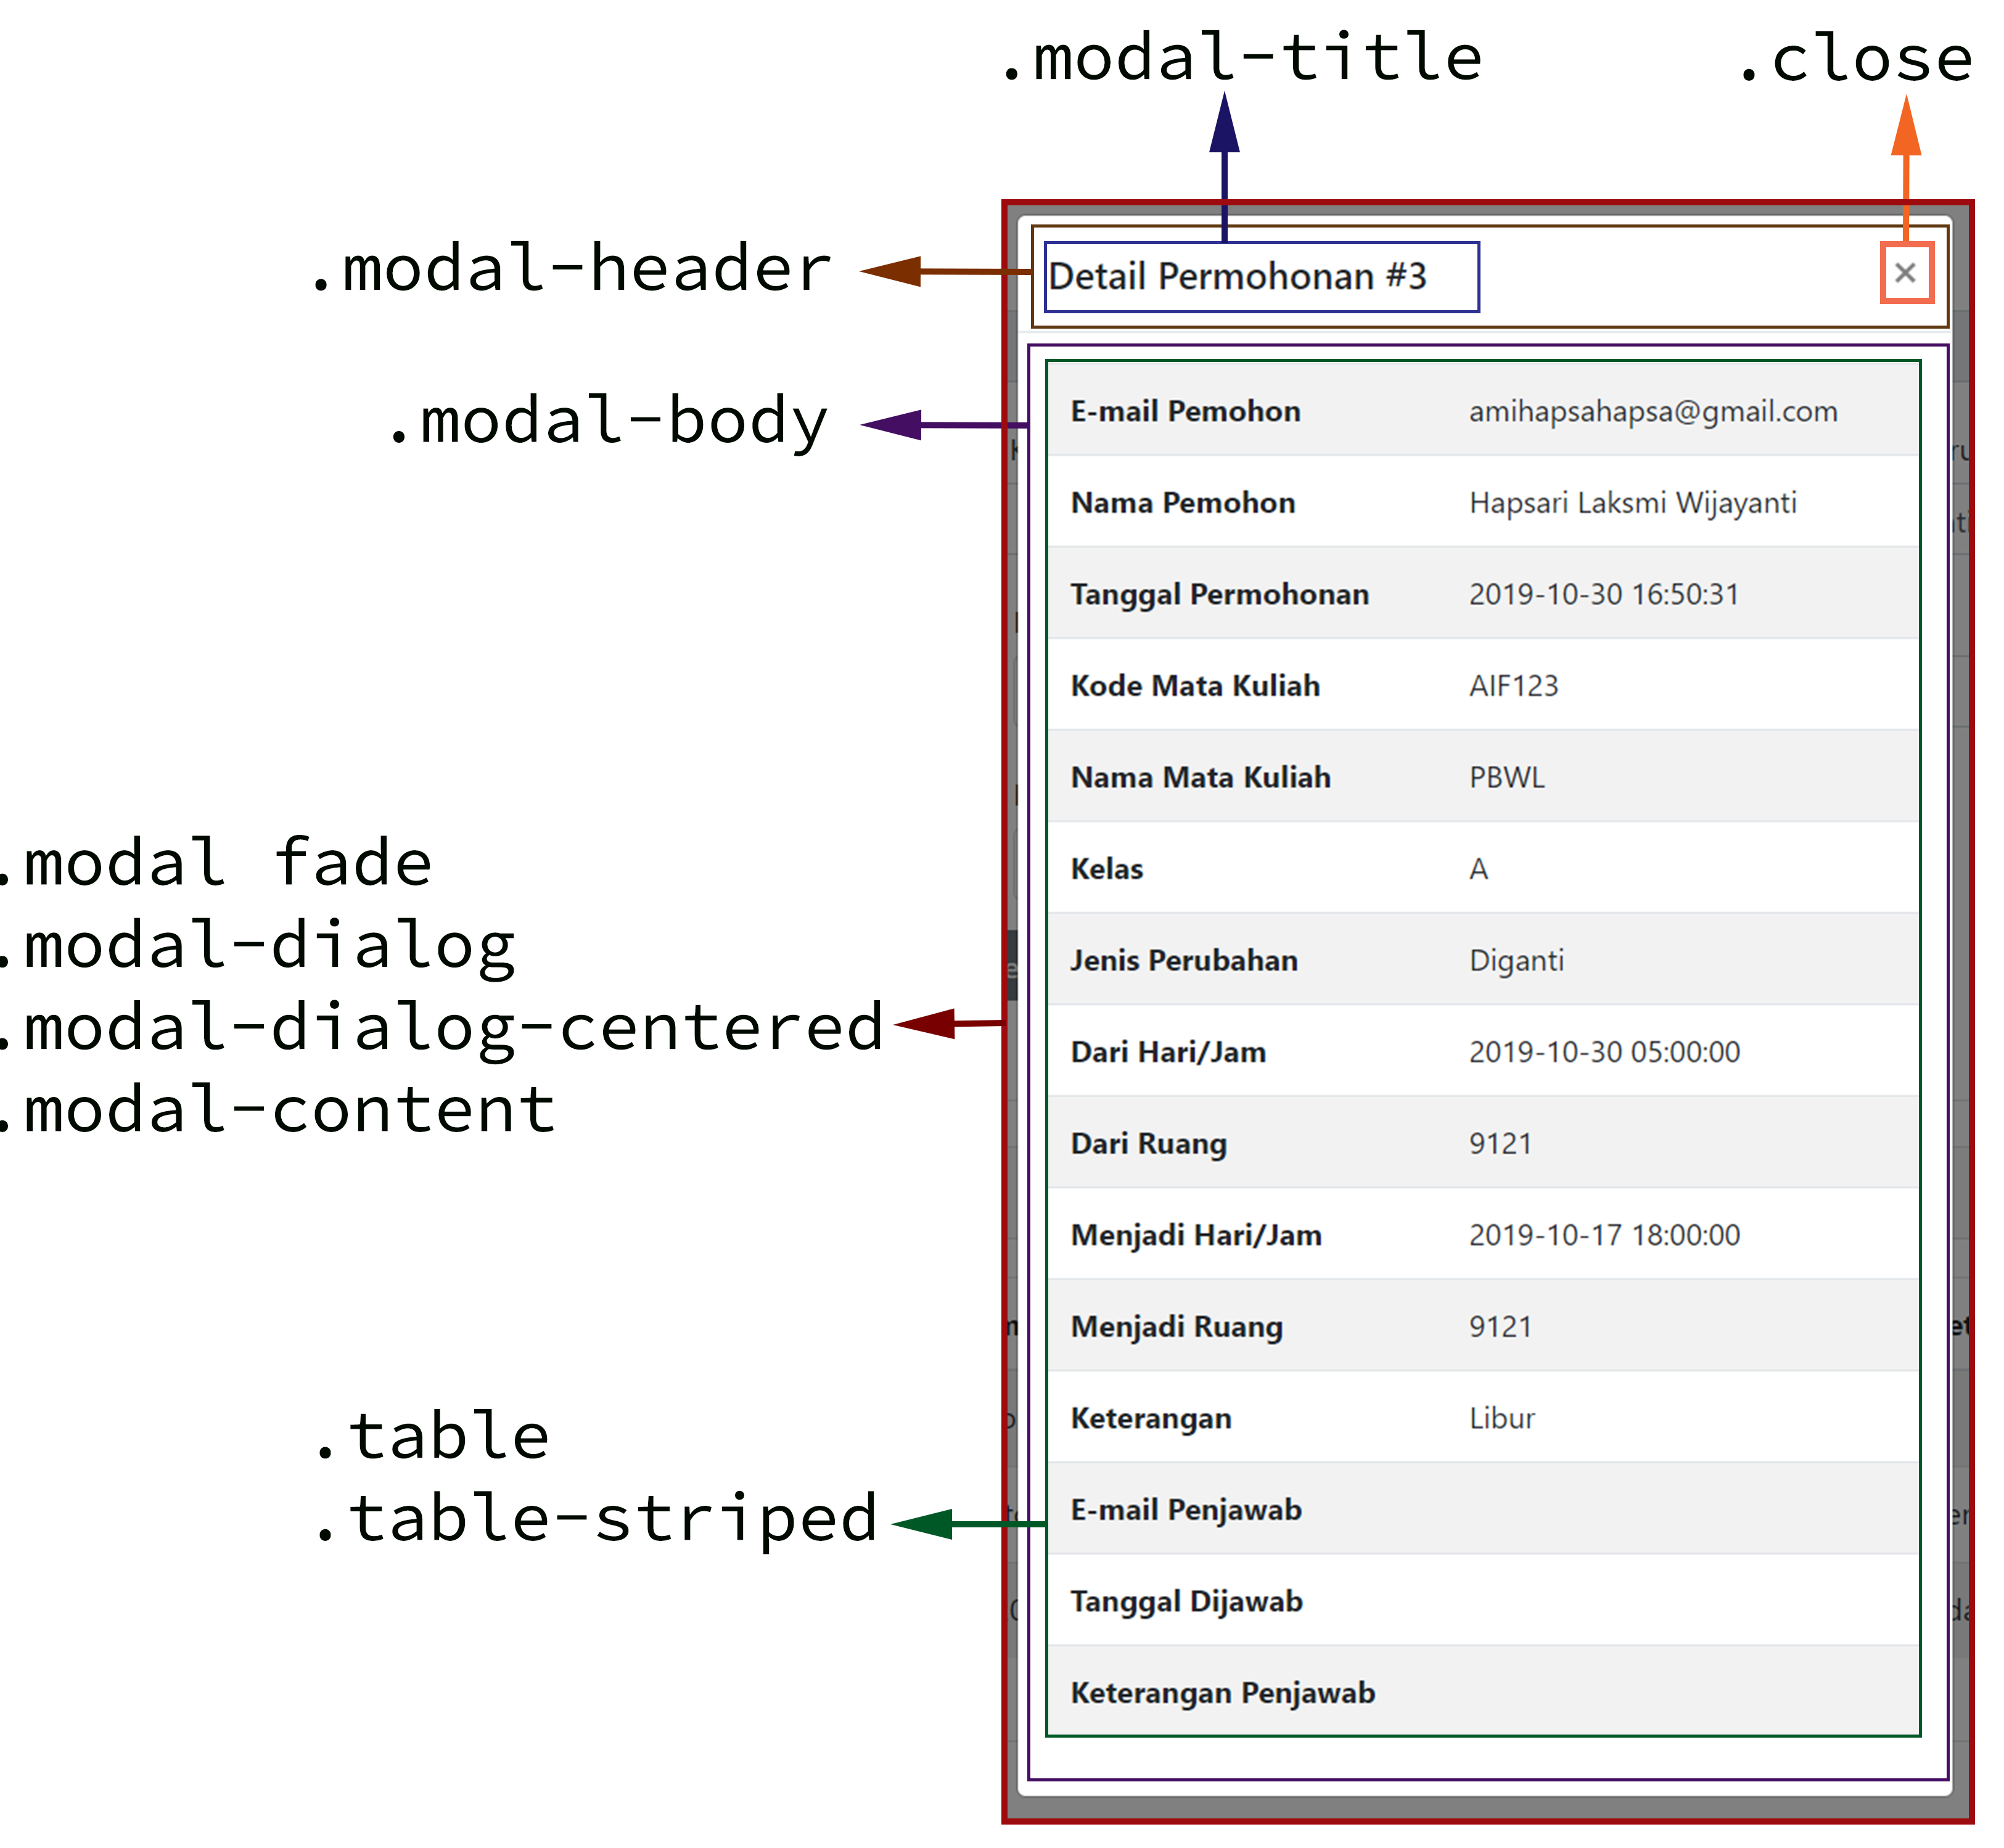
\includegraphics[width=\textwidth,height=\textheight,keepaspectratio]{bootstrap/konversi_modal_lihat_manajemen_perubahan_kuliah.png}
		\caption{Modal lihat.}
	\end{subfigure}	
	\begin{subfigure}[b]{0.45\linewidth} 
		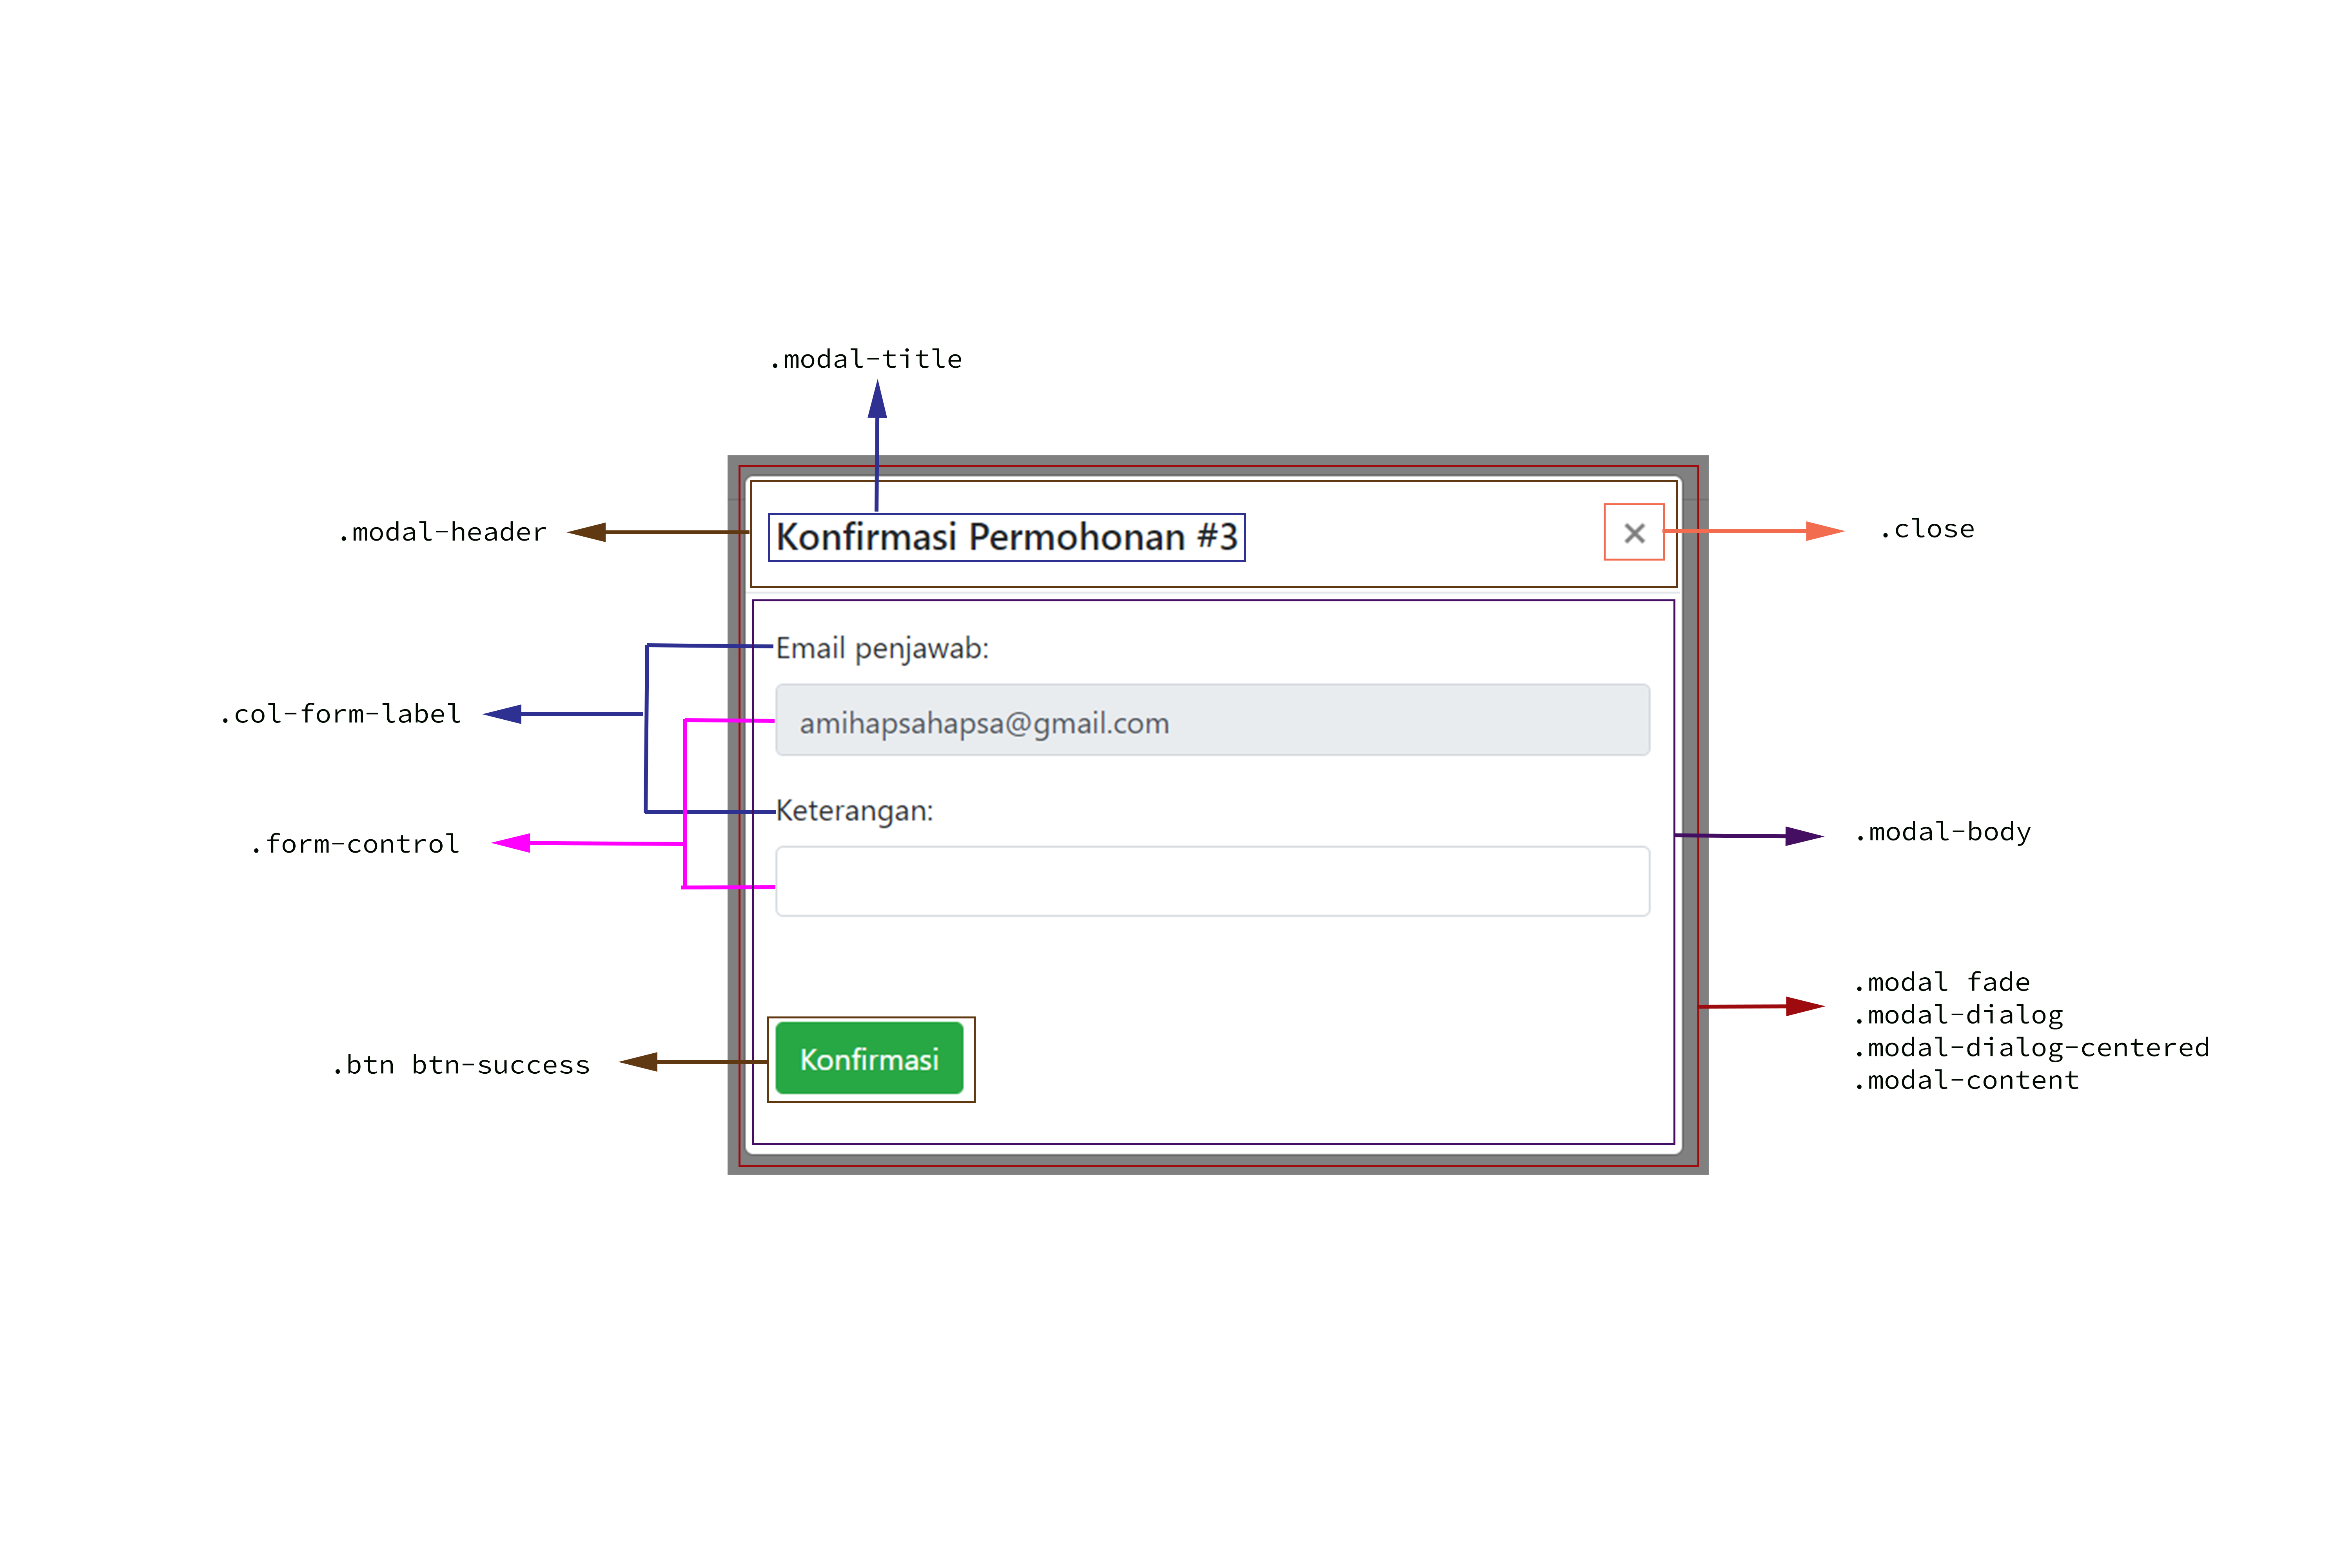
\includegraphics[width=\textwidth,height=\textheight,keepaspectratio]{bootstrap/konversi_modal_like_manajemen_perubahan_kuliah.png}
		\caption{Modal setuju.}
	\end{subfigure}
\end{figure}
\begin{figure}[H]	
	\centering
	\ContinuedFloat
	\begin{subfigure}[b]{0.45\linewidth}  
		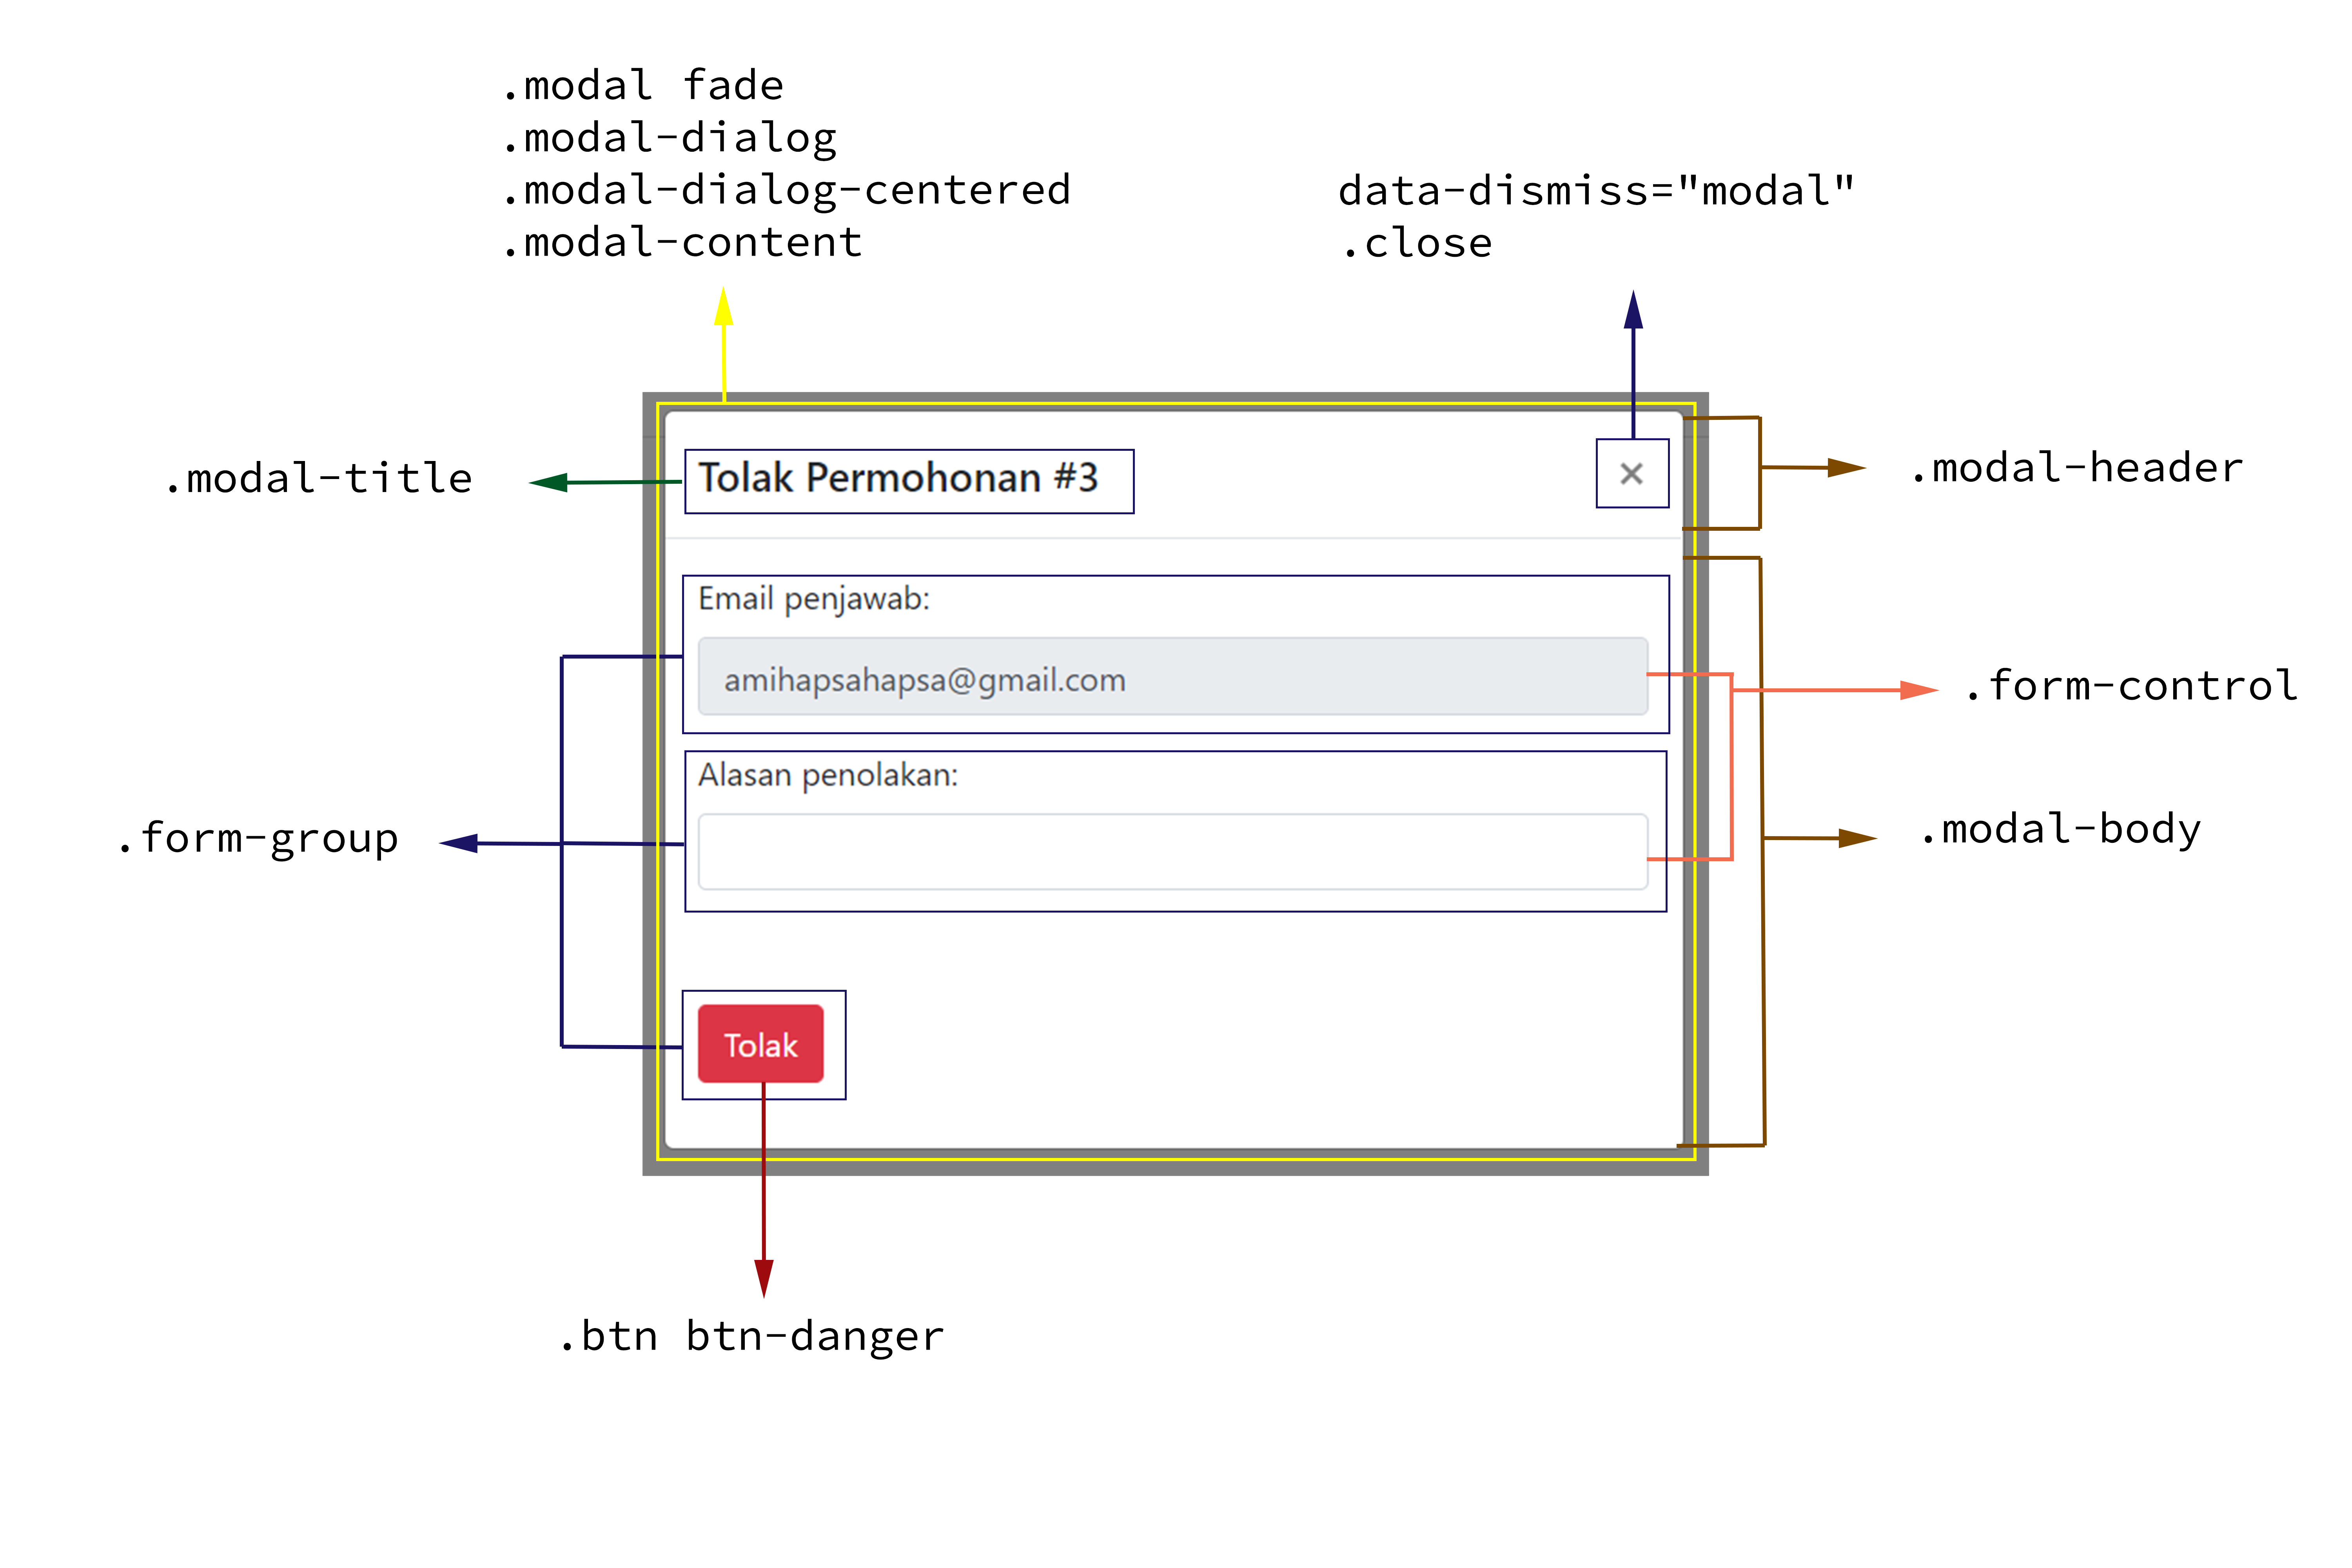
\includegraphics[width=\textwidth,height=\textheight,keepaspectratio]{bootstrap/konversi_modal_dislike_manajemen_perubahan_kuliah.png}
		\caption{Modal tolak.}
	\end{subfigure}
\end{figure}

\begin{figure}[H] 
	\centering
	\ContinuedFloat
	\begin{subfigure}[b]{0.45\linewidth}  
		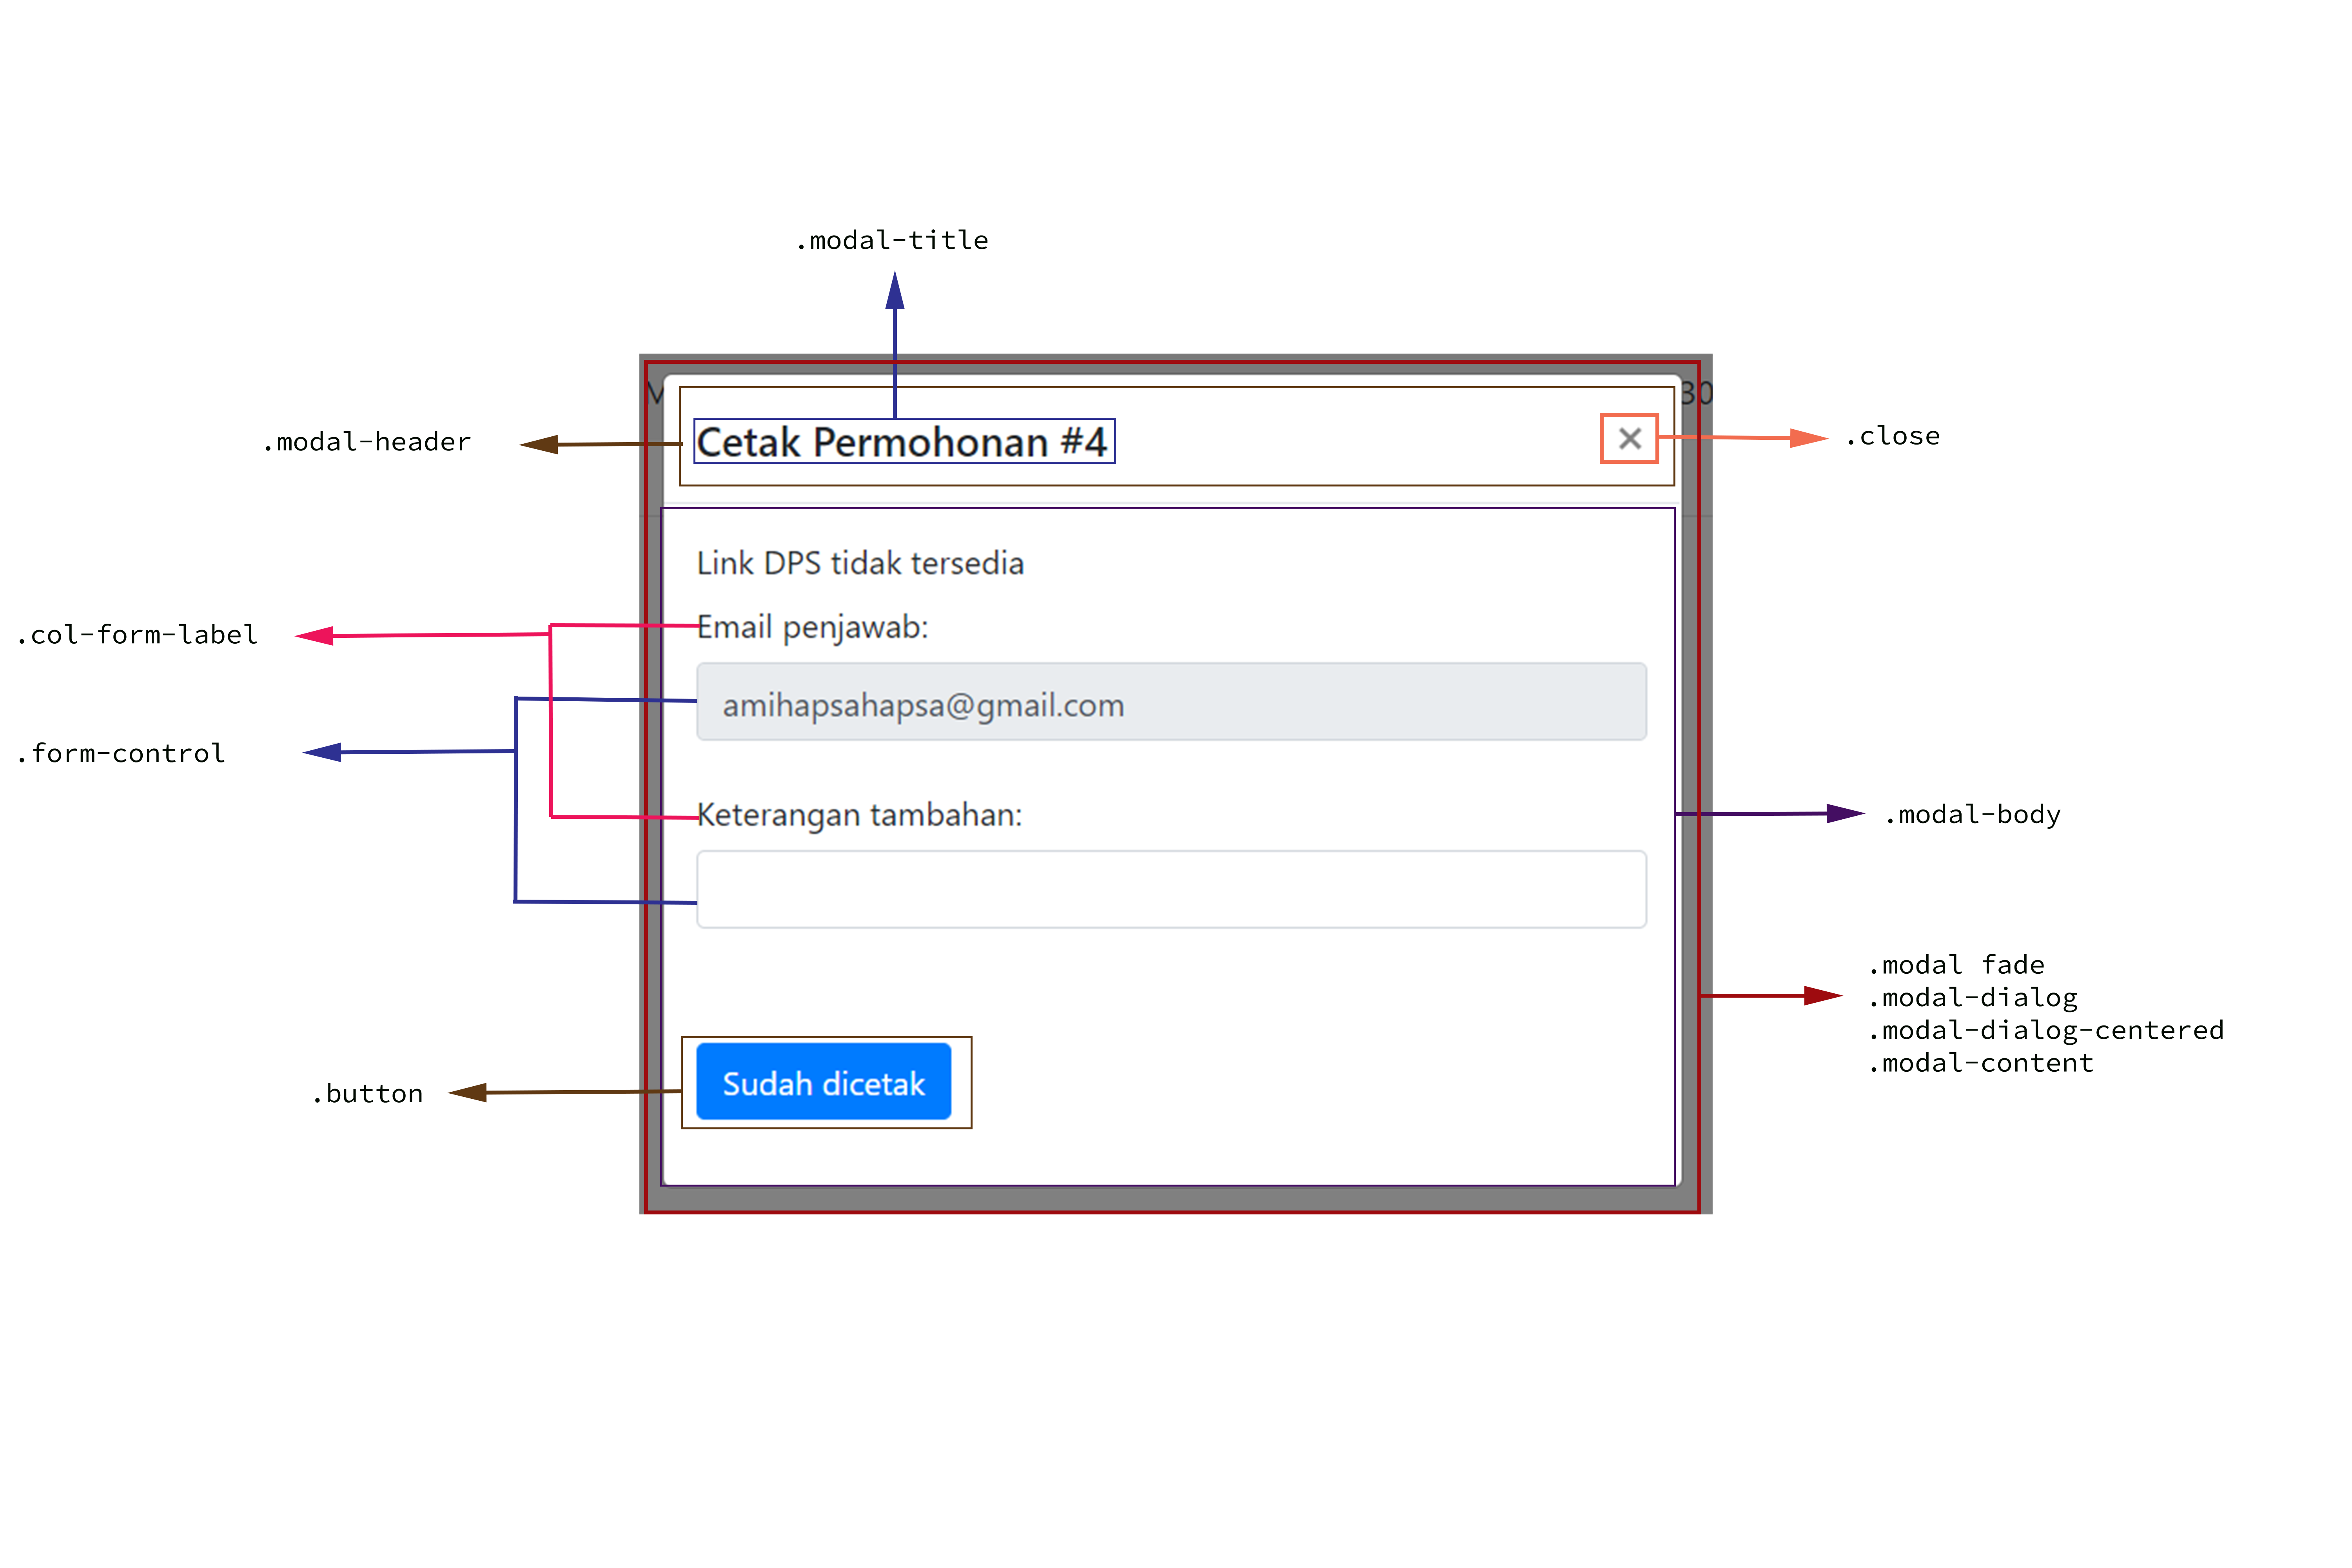
\includegraphics[width=\textwidth,height=\textheight,keepaspectratio]{bootstrap/konversi_modal_print_manajemen_cetak_transkrip.png}
		\caption{Modal print}
	\end{subfigure}	
	\begin{subfigure}[b]{0.45\linewidth}   
		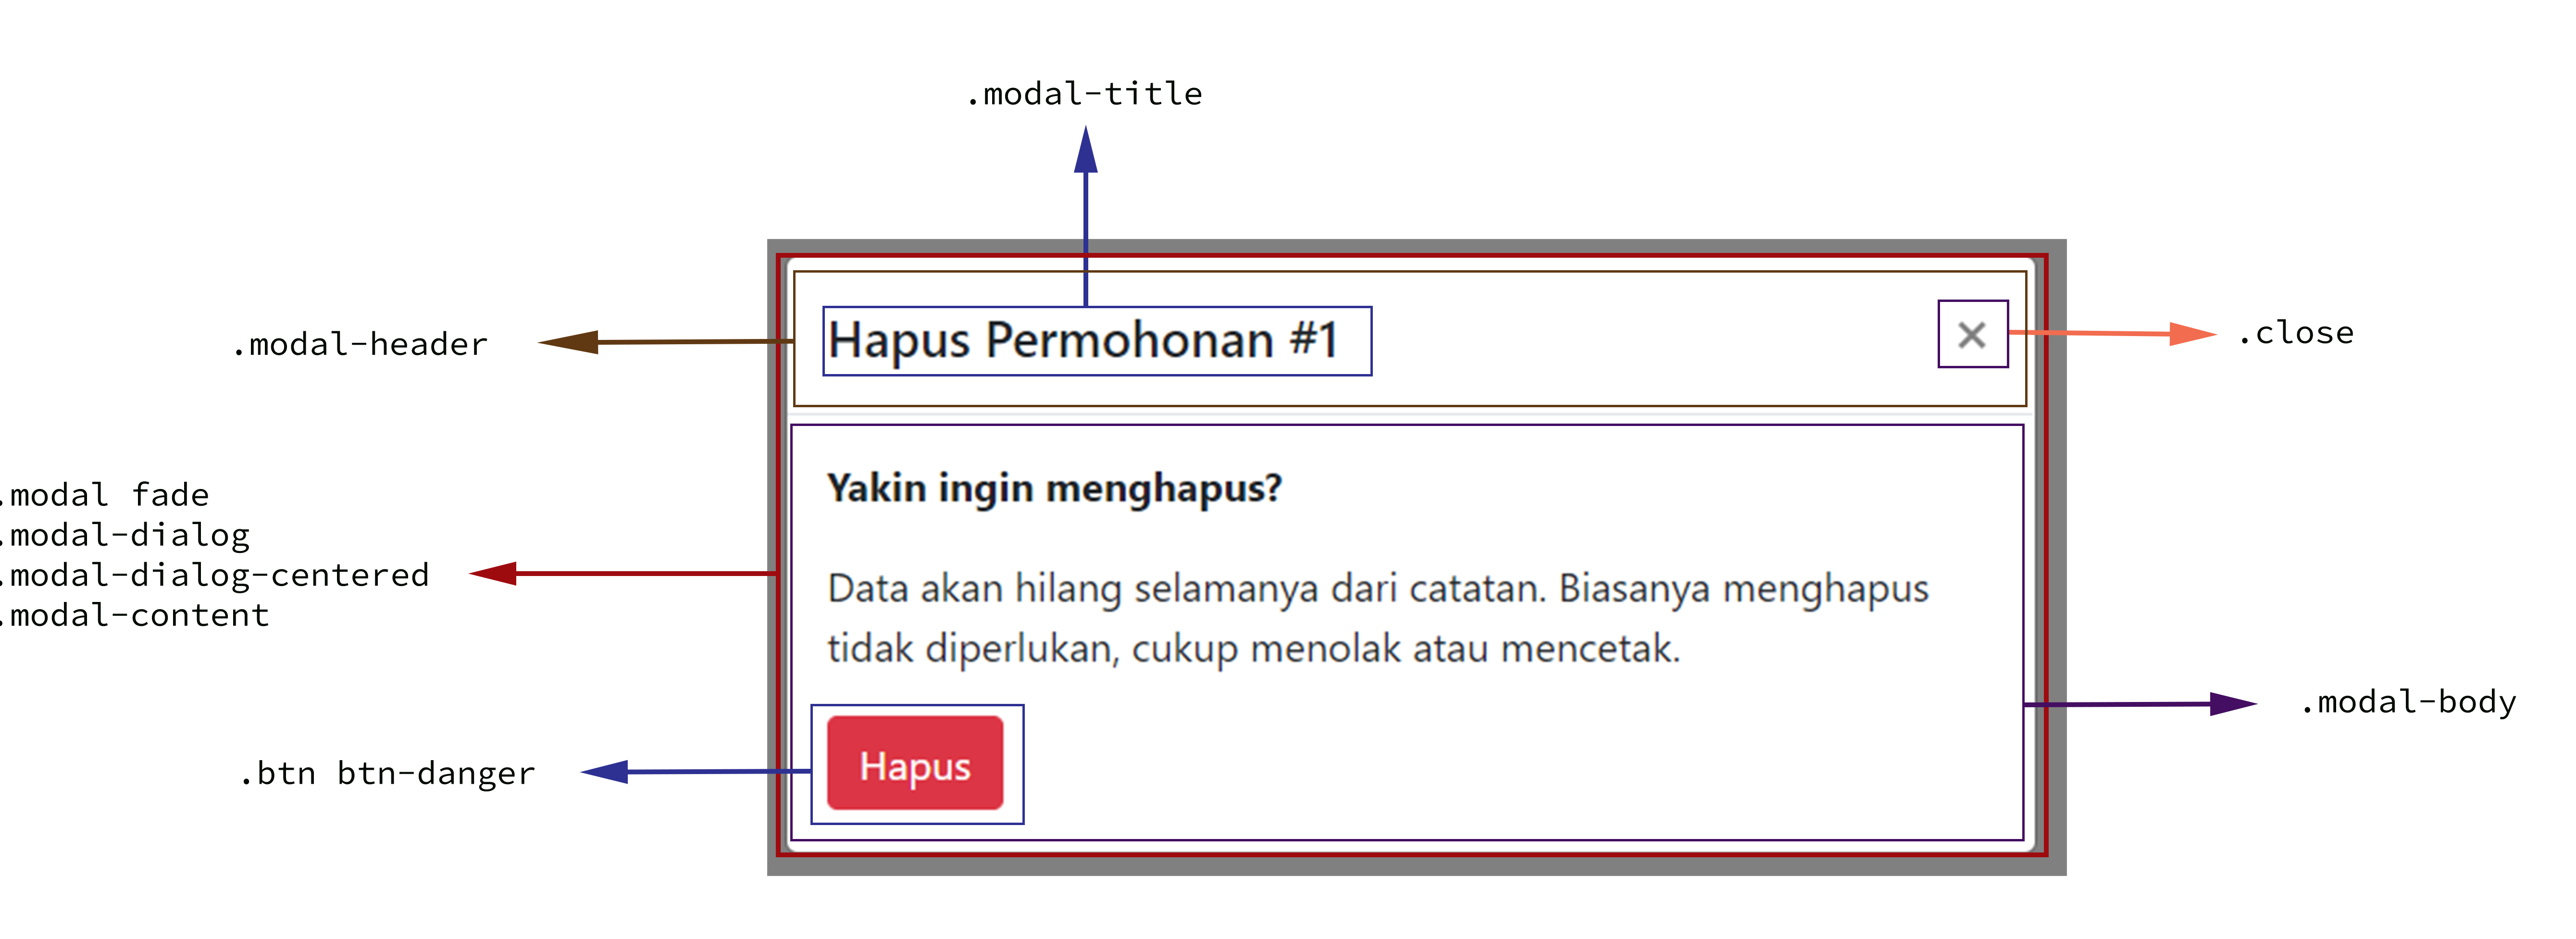
\includegraphics[width=\textwidth,height=\textheight,keepaspectratio]{bootstrap/konversi_modal_trash_manajemen_perubahan_kuliah.png}
		\caption{Modal hapus.}
	\end{subfigure}
\caption{Konversi modal pada halaman manajemen perubahan kuliah.}
\label{fig:konversiModalManajemenPerubahanKuliah}
\end{figure}

\noindent Pada tabel ~\ref{table:konversiModalManajemenPerubahanKuliah} menjelaskan kelas-kelas yang digunakan dalam komponen modal.
\begin{table}[H]
	\caption{Tabel konversi pada modal manajemen perubahan kuliah.}
	\begin{tabular}{| p{0.35\textwidth} | p{0.27\textwidth} | p{0.27\textwidth} |} 
		\hline
		\textbf{Jenis Komponen} & \textbf{Foundation 6} & \textbf{Bootstrap 4}  \\ [0.5ex] 
		\hline	
		Modal & \texttt{.reveal data-reveal} & \texttt{.modal-fade} \newline \texttt{.modal-dialog} \newline \texttt{.modal-dialog-centered} \newline \texttt{.modal-content} \\
		\hline
		Judul modal & - & \texttt{modal-title}\\
		\hline
		Isi modal & - & \texttt{modal-body}\\
		\hline
		Tutup modal & \texttt{.close-button} \newline \texttt{data-close} \newline \texttt{aria-label} & \texttt{.close}\\
		\hline	
		Tabel & \texttt{.stack} & \texttt{.table} \newline \texttt{.table-striped} \\[1ex]
		\hline
	\end{tabular}
	\label{table:konversiModalManajemenPerubahanKuliah}
\end{table}

\subsection{Halaman Entri Jadwal Dosen}
\subsubsection{Halaman Utama}
\noindent Gambar ~\ref{fig:konversiEntriJadwalDosen} menjelaskan komponen dalam website beserta penamaan kelas untuk Bootstrap 4 pada halaman entri jadwal dosen.\\
\begin{figure} [H]
	\centering  
	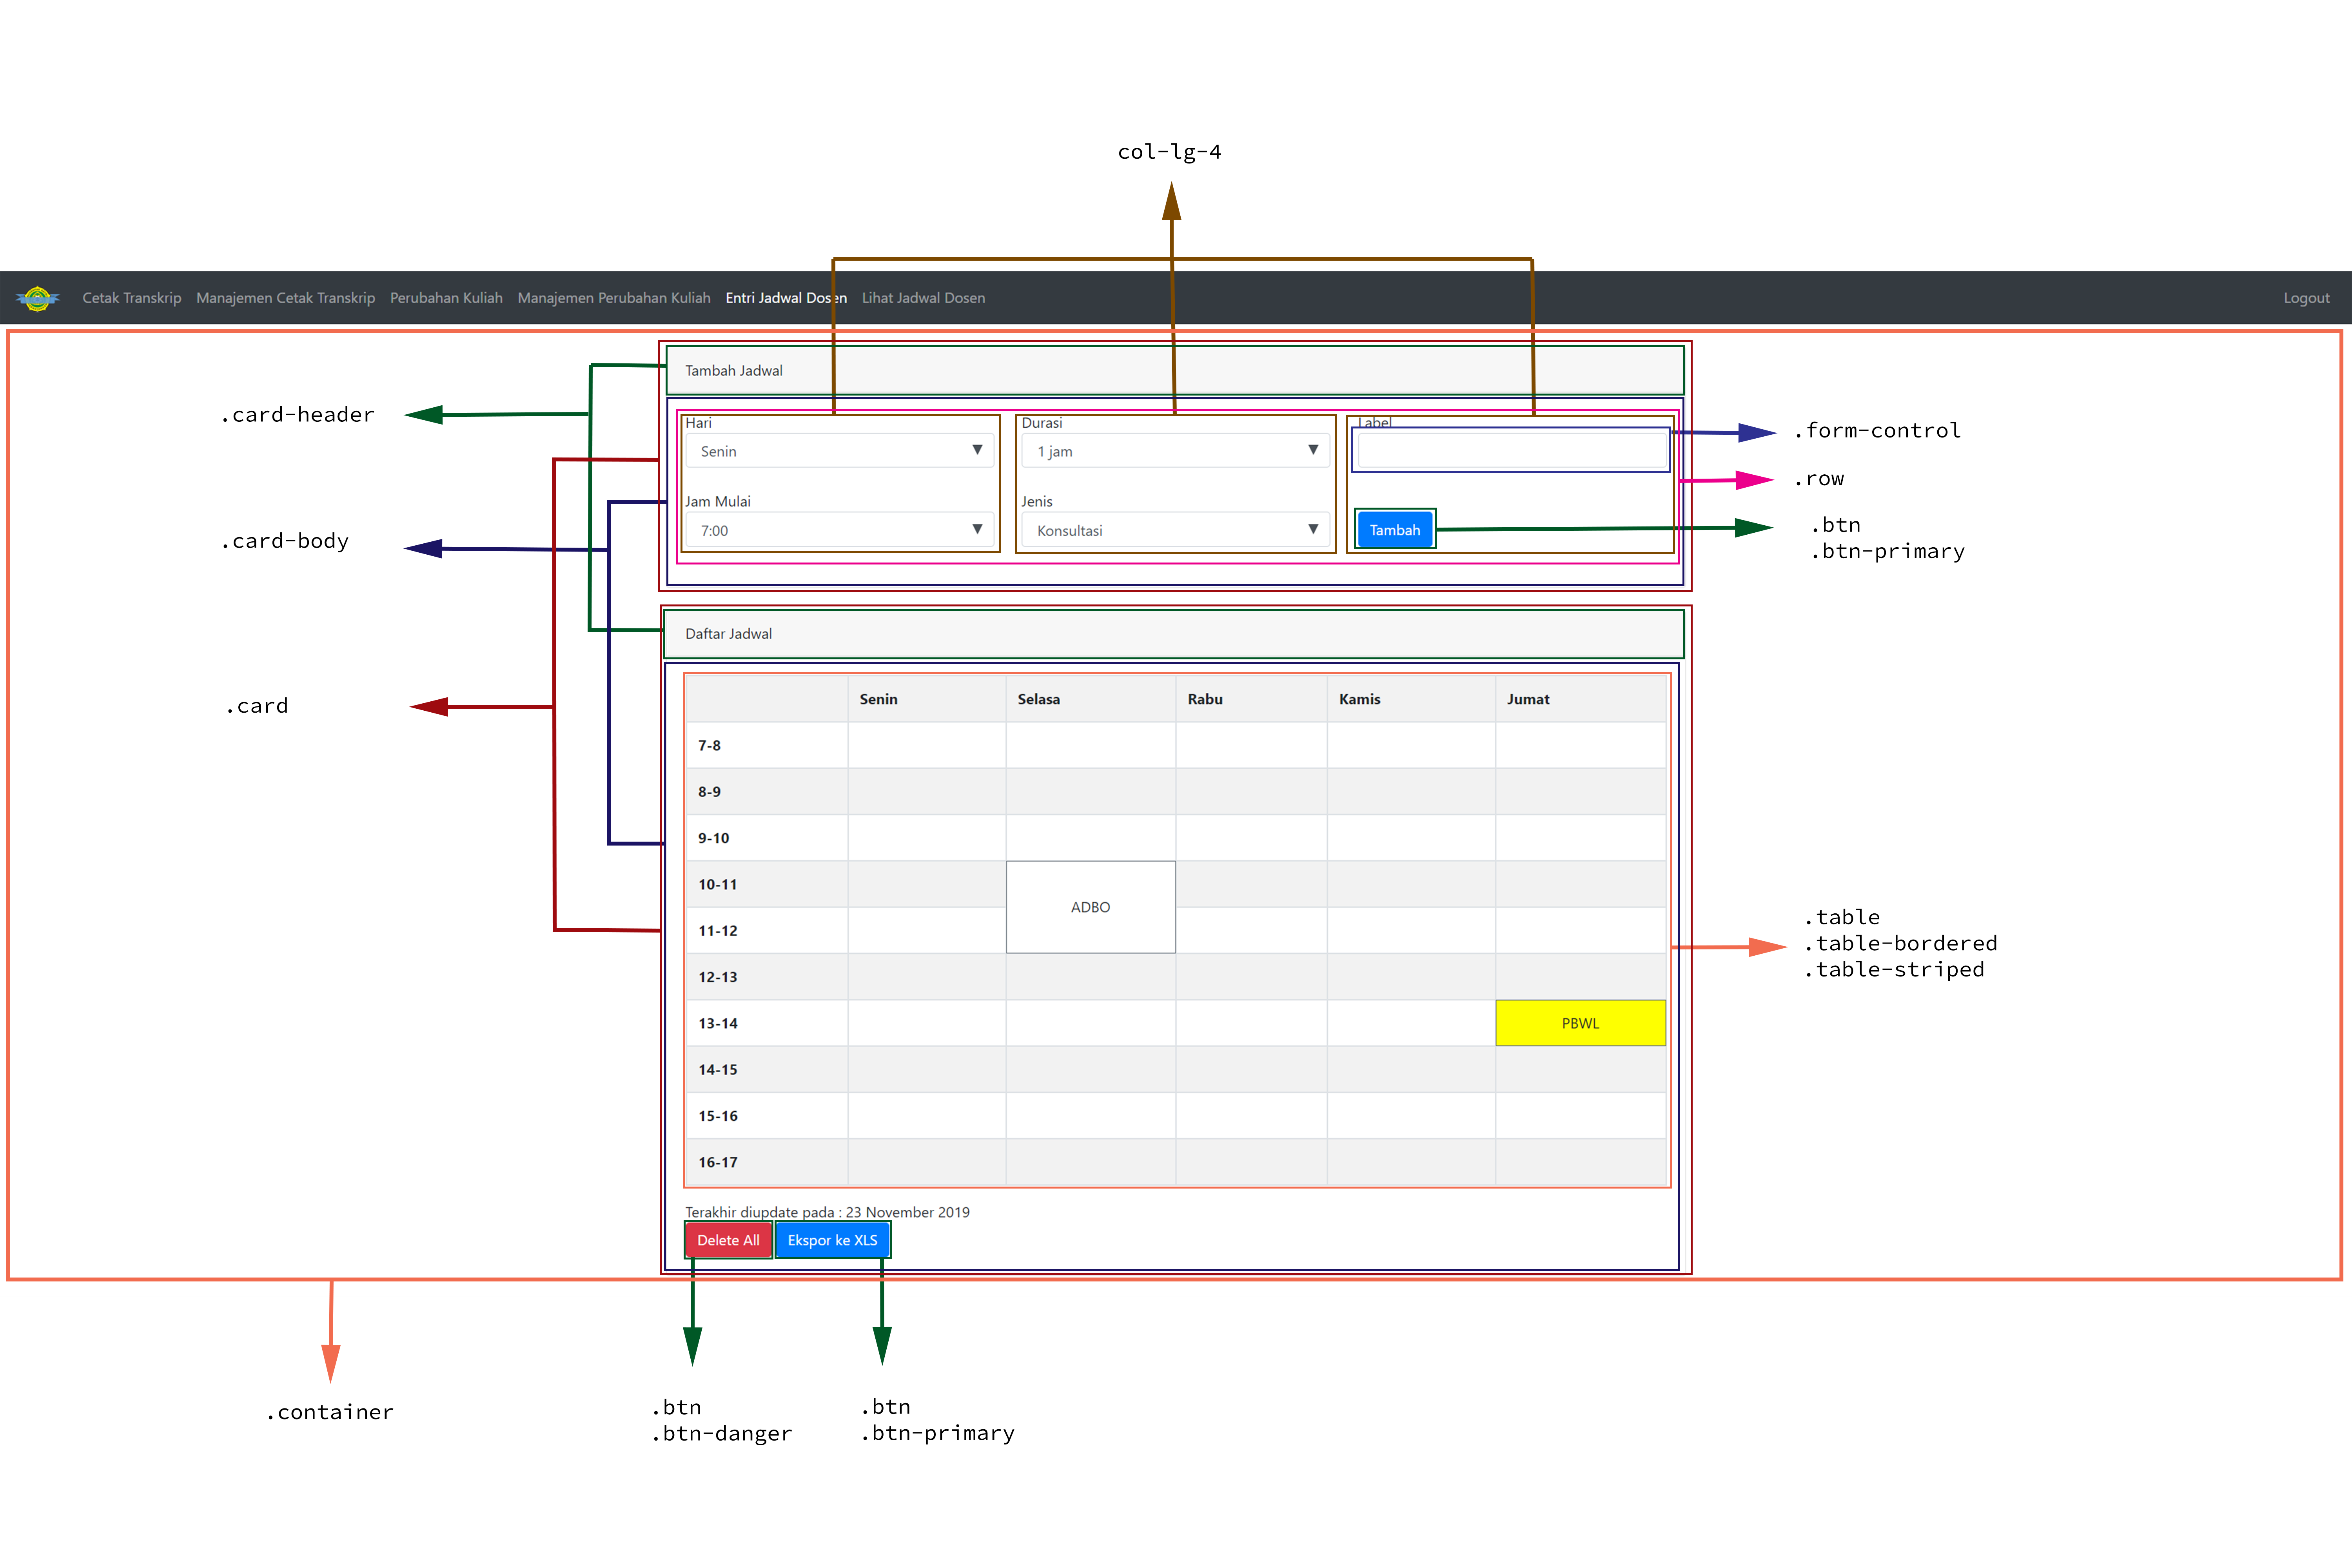
\includegraphics[width=\textwidth,height=\textheight,keepaspectratio]{bootstrap/konversi_tampilan_entri_jadwal_dosen.png}
	\caption{Konversi halaman entri jadwal dosen.}
	\label{fig:konversiEntriJadwalDosen}
\end{figure}

\noindent Perbandingan penggunaan kelas pada Foundation 6 dan Bootstrap 4 pada halaman entri jadwal dosen tertera pada tabel ~\ref{table:konversiEntriJadwalDosen}.\\
\begin{table}[H]
	\caption{Tabel konversi pada halaman entri jadwal dosen.}
	\begin{tabular}{| p{0.35\textwidth} | p{0.27\textwidth} | p{0.27\textwidth} |} 
		\hline
		\textbf{Jenis Komponen} & \textbf{Foundation 6} & \textbf{Bootstrap 4}  \\ [0.5ex] 
		\hline	
		Sistem Grid & \texttt{.row} \newline \texttt{.col} &   \texttt{.container} \newline \texttt{.row} \newline \texttt{.col} \\ 
		\hline	
		Border untuk konten & \texttt{.callout} &  \texttt{.card} \newline \texttt{.card-header} \newline \texttt{.card-body} \\
		\hline
		Form & - & \texttt{.form-control} \\	
		\hline		
		Link modal sesuai ID & \texttt{data-open} & \texttt{data-toggle} \newline \texttt{data-target}\\
		\hline	
		Tabel & \texttt{.stack} & \texttt{.table} \newline \texttt{.table-bordered} \newline \texttt{.table table-striped}  \\[1ex]
		\hline	
	\end{tabular}
	\label{table:konversiEntriJadwalDosen}
\end{table}

\subsubsection{Modal: Edit}
\noindent Gambar ~\ref{fig:konversiEditEntriJadwalDosen} menjelaskan komponen dalam website beserta penamaan kelas untuk Bootstrap 4 pada modal entri jadwal dosen.\\
\begin{figure} [H]
	\centering  
	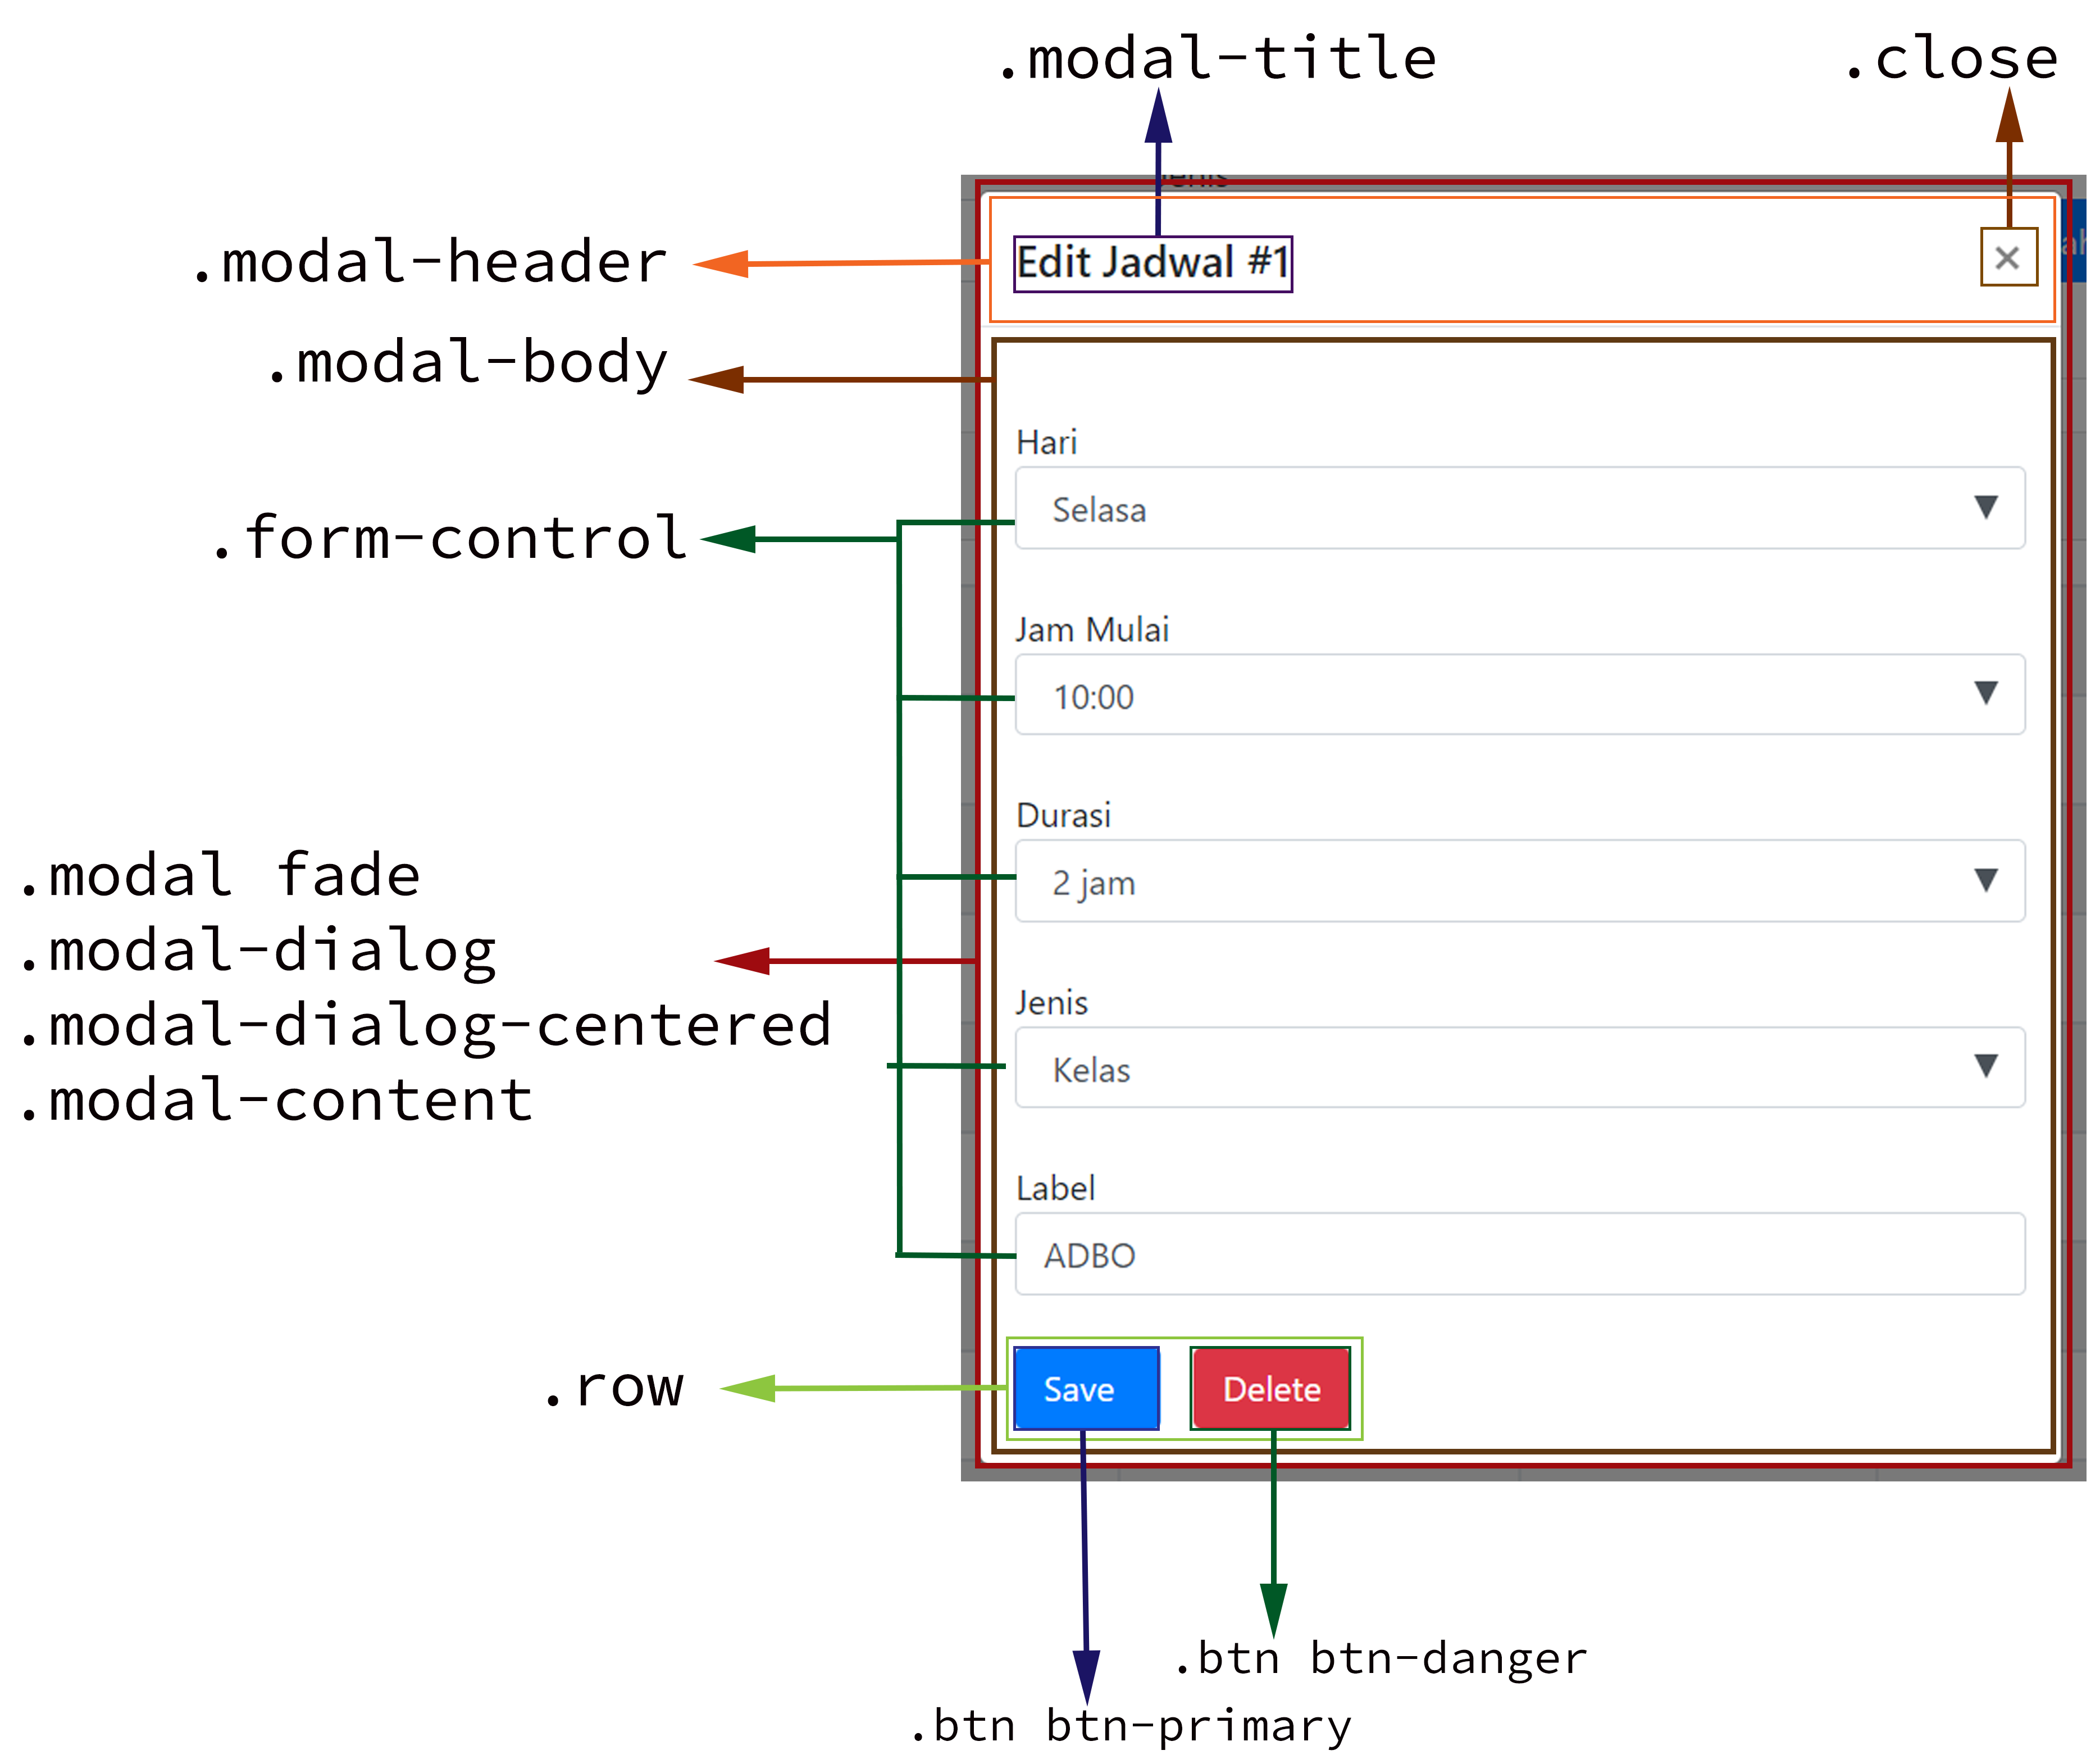
\includegraphics[width=0.6\textwidth,height=\textheight,keepaspectratio]{bootstrap/konversi_modal_edit_jadwal_entri_jadwal_dosen.png}
	\caption{Konversi modal edit pada halaman entri jadwal dosen.}
	\label{fig:konversiEditEntriJadwalDosen}
\end{figure}

\noindent Perbandingan penggunaan kelas pada Foundation 6 dan Bootstrap 4 pada modal edit entri jadwal dosen tertera pada tabel ~\ref{table:konversiEditEntriJadwalDosen}.\\
\begin{table}[H]
	\caption{Tabel konversi pada modal edit pada halaman entri jadwal dosen.}
	\begin{tabular}{| p{0.35\textwidth} | p{0.27\textwidth} | p{0.27\textwidth} |} 
		\hline
		\textbf{Jenis Komponen} & \textbf{Foundation 6} & \textbf{Bootstrap 4}  \\ [0.5ex] 
		\hline	
		Grid & \texttt{.row} & \texttt{.row} \newline \texttt{.container} \\
		\hline
		Ukuran Grid & \texttt{.large-*-columns} & \texttt{.col-lg-*}\\
		\hline	
		Modal & \texttt{.reveal} \newline \texttt{data-reveal} & \texttt{.modal-fade} \newline \texttt{.modal-dialog} \newline \texttt{.modal-dialog-centered} \newline \texttt{.modal-content} \\
		\hline
		Judul modal & - & \texttt{modal-title}\\
		\hline
		Isi modal & - & \texttt{modal-body}\\
		\hline
		\textit{Form} & - & \texttt{form-control}\\
		\hline
		Tombol berwarna merah & \texttt{.alert button} & \texttt{.btn btn-danger}\\
		\hline		
		Tombol berwarna biru & \texttt{.button}  & \texttt{.btn btn-primary}\\
		\hline
		Tabel & \texttt{.table-scroll} & \texttt{.table} \newline \texttt{.table-striped} \\[1ex]
		\hline
	\end{tabular}
	\label{table:konversiEditEntriJadwalDosen}
\end{table}

\subsection{Halaman Lihat Jadwal Dosen}
\noindent Gambar ~\ref{fig:konversiLihatJadwalDosen} menjelaskan komponen dalam website beserta penamaan kelas untuk Bootstrap 4 pada halaman lihat jadwal dosen.\\

\begin{figure} [H]
	\centering  
	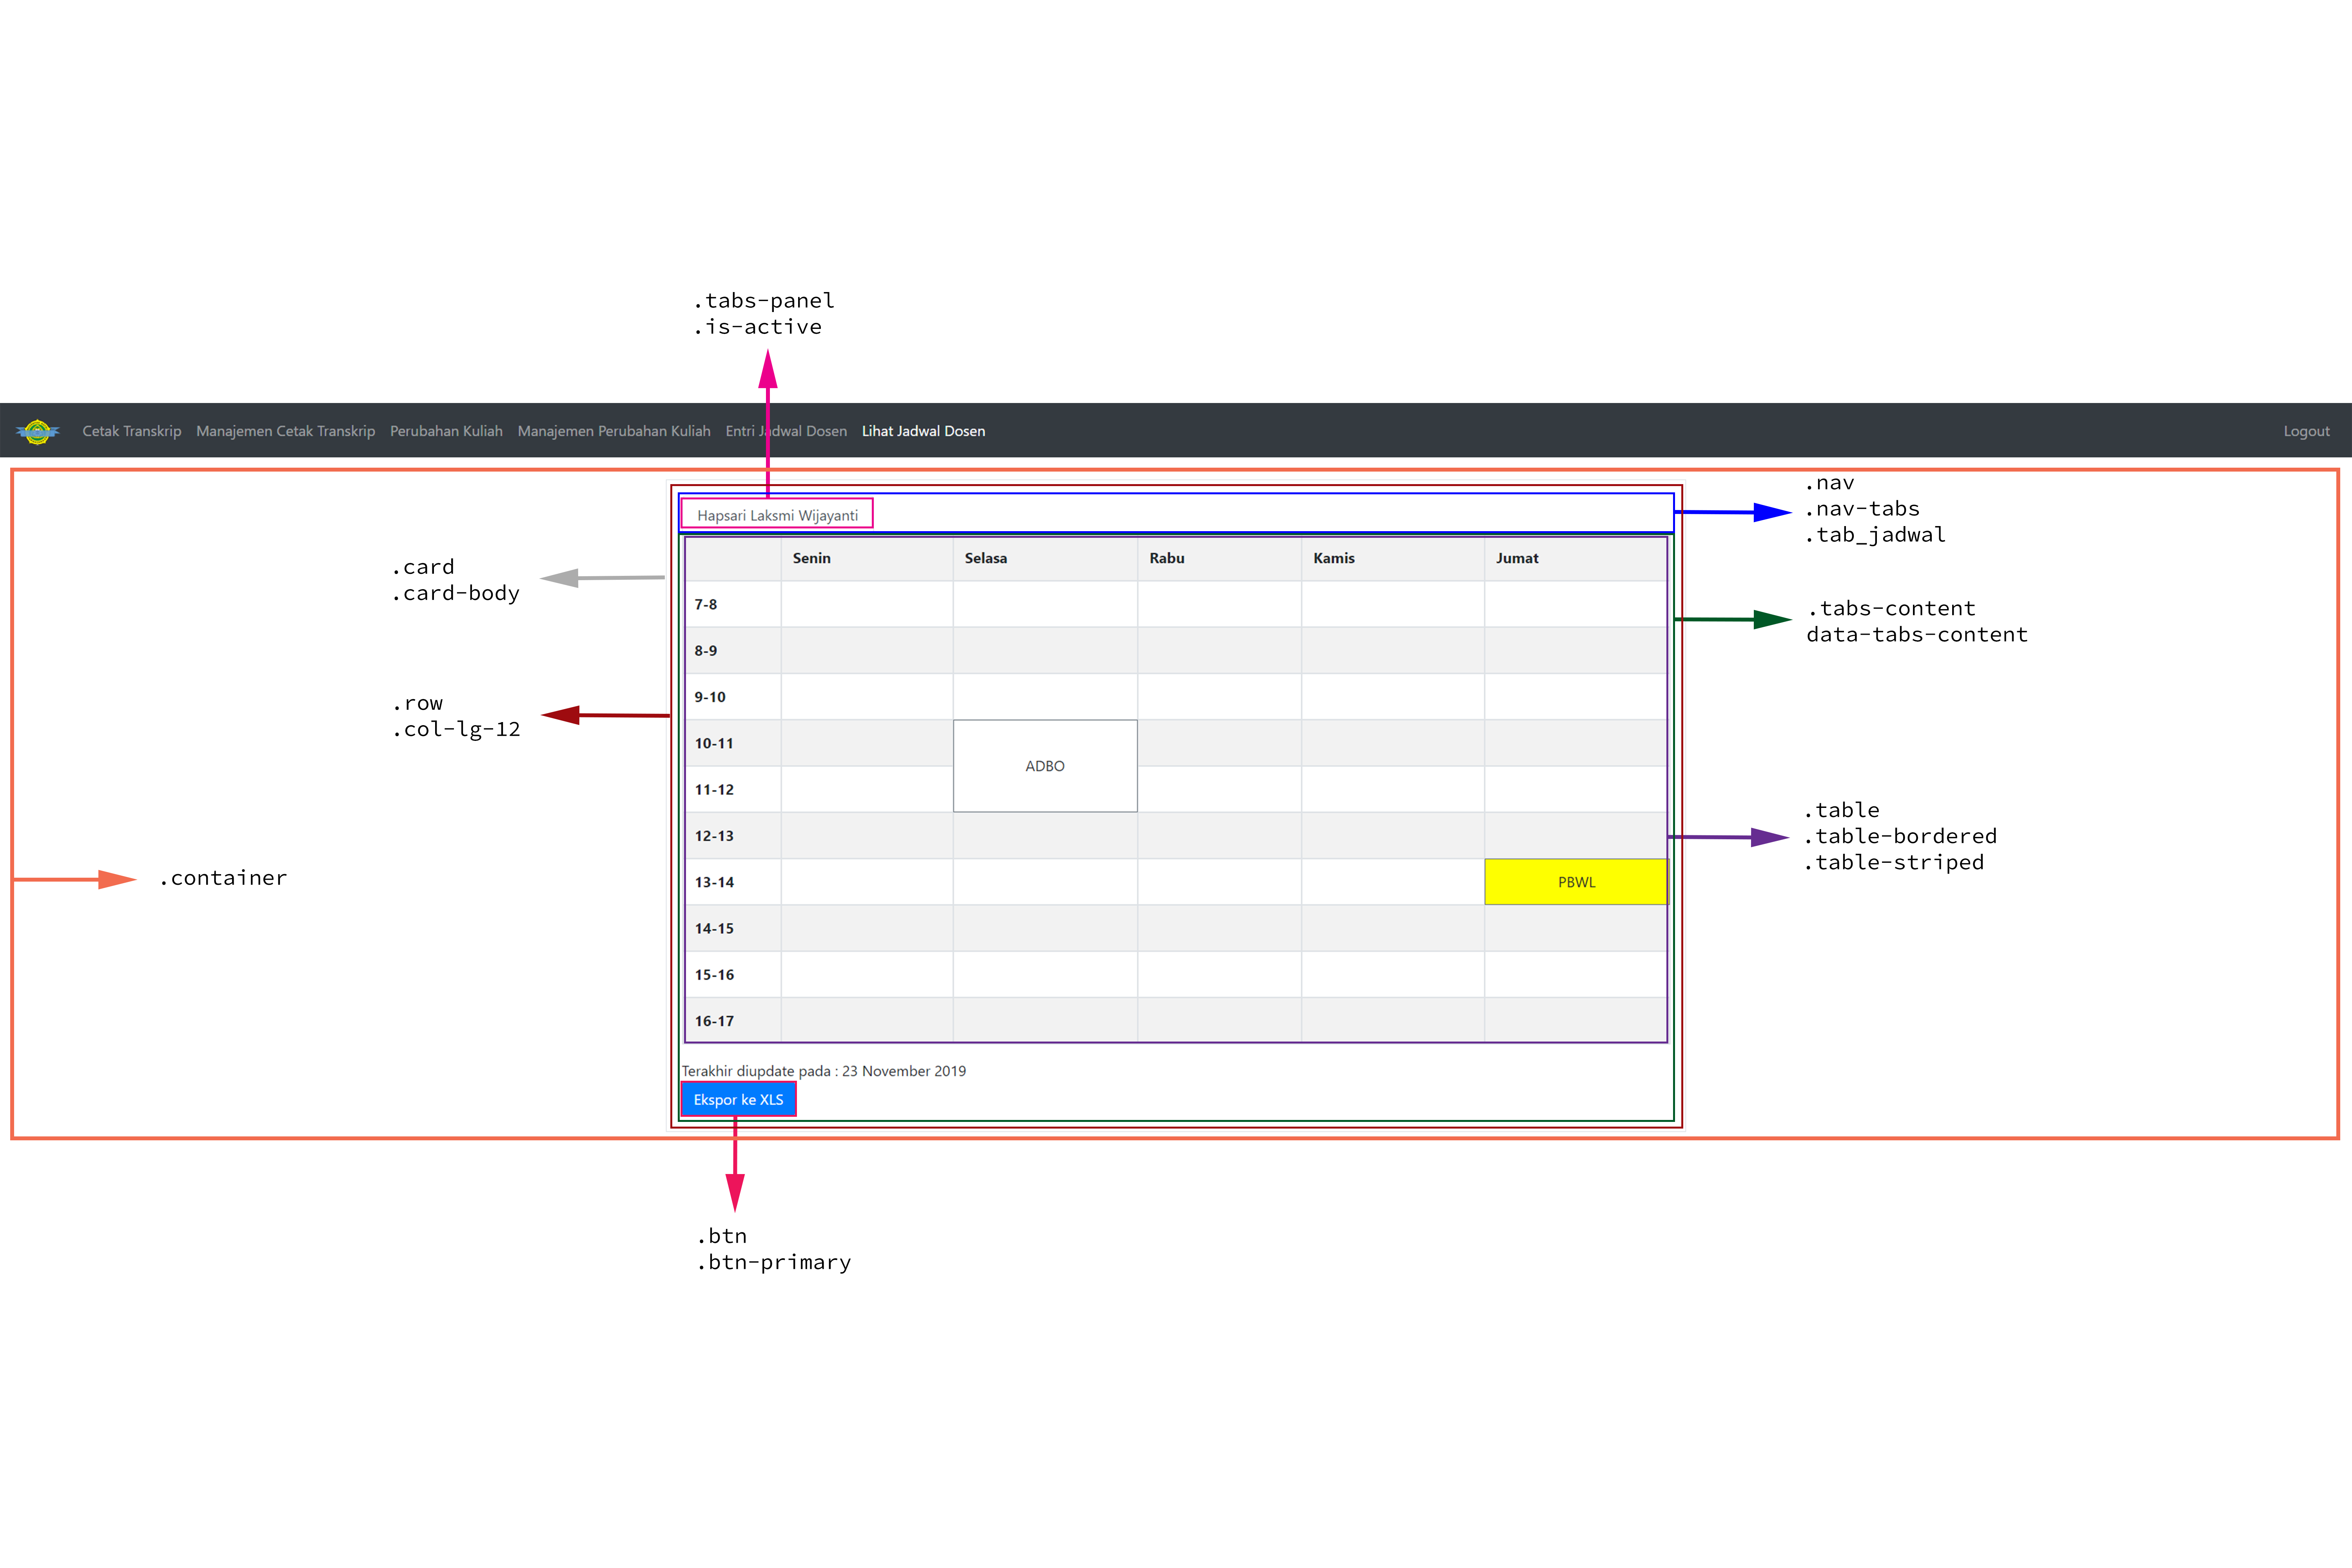
\includegraphics[width=\textwidth,height=\textheight,keepaspectratio]{bootstrap/konversi_lihat_jadwal_dosen.png}
	\caption{Konversi modal lihat jadwal dosen.}
	\label{fig:konversiLihatJadwalDosen}
\end{figure}

\noindent Perbandingan penggunaan kelas pada Foundation 6 dan Bootstrap 4 pada halaman lihat jadwal dosen tertera pada tabel ~\ref{table:konversiLihatJadwalDosen}.\\
 
\begin{table}[H]
	\caption{Tabel konversi kelas pada lihat jadwal dosen.}
	\begin{tabular}{| p{0.35\textwidth} | p{0.27\textwidth} | p{0.27\textwidth} |} 
		\hline
		\textbf{Jenis Komponen} & \textbf{Foundation 6} & \textbf{Bootstrap 4}  \\ [0.5ex]
		\hline	
		Sistem Grid & \texttt{.row} & \texttt{.container}  \\ 
		&\texttt{.col} & \texttt{.row}\\
		\hline	
		Judul \textit{tabs} & \texttt{.tabs}  &\texttt{.nav} \\
		&\texttt{data-tabs}&\texttt{.nav-tabs}\\
		&&\texttt{tab-jadwal}\\
		\hline
		Isi \textit{tabs} &\texttt{.tabs-content} & \texttt{.tabs-content}  \\
		&\texttt{data-tabs-content} & \texttt{data-tabs-content} \\
		\hline
		\textit{Tabs active} &\texttt{.tabs-title}  & \texttt{.tab-panel}  \\
		&\texttt{.is-active}&\texttt{.is-active}\\
		\hline	
		Tabel & \texttt{.stack} &\texttt{.table} \\
		&&  \texttt{.table table-striped} \\
		&&\texttt{.table-bordered}  \\
		\hline
		Tombol berwarna biru & \texttt{.button} & \texttt{.btn btn-primary}\\ [1ex]
		\hline		
	\end{tabular}
	\label{table:konversiLihatJadwalDosen}
\end{table}